\documentclass[11pt]{article}
\usepackage[letterpaper,margin=1in]{geometry}
\usepackage{fontspec}
\setmainfont{Latin Modern Roman}
\setsansfont{Latin Modern Sans}
\setmonofont{DejaVu Sans Mono}[Scale=0.78]
\usepackage{amsmath,amssymb,amsthm,mathtools}
\usepackage{microtype,booktabs,array,tabularx,longtable,enumitem,xcolor,fvextra,needspace}
\usepackage{cite}
\usepackage{tikz,pgfplots}
\usetikzlibrary{arrows.meta,positioning,calc,shapes.geometric,fit,backgrounds}
\pgfplotsset{compat=1.18}
\usepackage[unicode,colorlinks=true,linkcolor=blue!40!black,citecolor=blue!40!black,urlcolor=blue!40!black]{hyperref}
\mathchardef\UrlBigBreakPenalty=10000
\hypersetup{pdftitle={Exact Sampling from Neural Networks: Depth, Attention, and Decoding},pdfauthor={Samuel Mausberg}}
\newtheorem{theorem}{Theorem}[section]
\newtheorem{lemma}[theorem]{Lemma}
\newtheorem{proposition}[theorem]{Proposition}
\newtheorem{corollary}[theorem]{Corollary}
\theoremstyle{definition}
\newtheorem{definition}[theorem]{Definition}
\theoremstyle{remark}
\newtheorem{remark}[theorem]{Remark}
\newcommand{\E}{\mathbb E}
\newcommand{\PP}{\mathbb P}
\newcommand{\R}{\mathbb R}
\newcommand{\N}{\mathbb N}
\newcommand{\sech}{\operatorname{sech}}
\newcommand{\poly}{\operatorname{poly}}
\newcommand{\sgn}{\operatorname{sgn}}
\newcommand{\Maj}{\operatorname{Maj}}
\newcommand{\Bern}{\operatorname{Bern}}
\newcommand{\Pois}{\operatorname{Pois}}
\newcommand{\bits}{\mathcal B}
\newcommand{\cost}{\mathcal T}
\newcommand{\queries}{\mathcal Q}
\DeclareMathOperator{\artanh}{artanh}
\DeclareMathOperator{\TV}{TV}
\DeclareMathOperator{\RMS}{RMSNorm}
\DeclareMathOperator{\GELU}{GELU}
\DeclareMathOperator{\SiLU}{SiLU}
\setlist{nosep,leftmargin=1.6em}
\setlength{\emergencystretch}{2em}
\setlength{\parskip}{2pt}
\linespread{1.04}
\numberwithin{equation}{section}
\newcolumntype{Y}{>{\raggedright\arraybackslash}X}
\title{Exact Sampling from Neural Networks:\\Depth, Attention, and Decoding}
\author{Samuel Mausberg\\{\normalsize Independent Researcher}}
\date{8 October 2026\quad\textit{Full version}}
\begin{document}
\maketitle

\begin{abstract}
One random output can require much less work than numerical evaluation.
We study exact neural sampling, counting input probes, random bits,
arithmetic, and every precision refinement.

For dense tanh networks with absolute row sums at most one, weight
preprocessing permits polylogarithmic expected sampling work at
logarithmic depth. With zero biases, the sharp query scale is the square
root of depth at every fixed first-layer rank, and also at arbitrary
rank when a column envelope is bounded. The unrestricted gap between
square-root and linear query cost remains open.

Prefill changes attention. We construct an appendable cache index and a
complete exact decoder with positive RMSNorm stabilizers. Its expected
work is polynomial in model size and $\log T$ when each layer has a
common affine key space of fixed rank and the context has length $T$.
The decoder's polynomial degree grows with rank.
These bounds give no useful speed prediction at the large ranks of
ordinary models. A completely fixed full-rank model still has a formal
polylogarithmic context bound, with potentially enormous constants.

The decoder maintains finite Taylor moments, prepares precision in the
background, and charges rare complete refinements by their probability.
Its cost includes neural key and value creation. Without a context index,
standard scaling can force linear positional search; arbitrary indexed
queries face a conditional barrier in growing dimension. We also prove
exact normalization factories and a matching law for an explicit
additive-residual family. A checkpoint section gives the certificates
and cost formulas needed to apply each positive result.
\end{abstract}

\begin{figure}[ht]
\centering
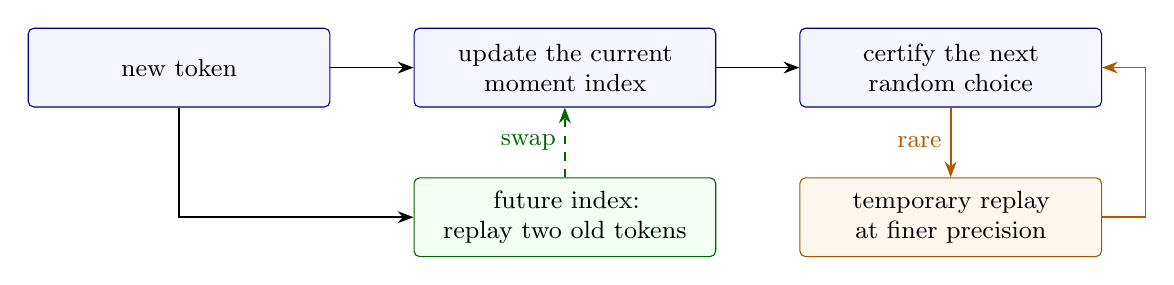
\begin{tikzpicture}[
 >=Stealth,font=\small,
 box/.style={draw=blue!55!black,fill=blue!4,rounded corners=2pt,
             minimum height=10mm,align=center,text width=3.55cm,
             inner sep=4pt},
 edge/.style={->,semithick}]
 \node[box] (token) at (0,0) {new token};
 \node[box] (current) at (4.9,0) {update the current\\moment index};
 \node[box] (sample) at (9.8,0) {certify the next\\random choice};
 \node[box,fill=green!5,draw=green!40!black] (future) at (4.9,-1.9)
   {future index:\\replay two old tokens};
 \node[box,fill=orange!7,draw=orange!65!black] (refine) at (9.8,-1.9)
   {temporary replay\\at finer precision};
 \draw[edge] (token)--(current);
 \draw[edge] (current)--(sample);
 \draw[edge] (token.south) |- (future.west);
 \draw[edge,green!40!black,dashed] (future.north)--
   node[left,inner sep=3pt] {swap}(current.south);
 \draw[edge,orange!70!black] (sample.south)--
   node[left,inner sep=3pt] {rare}(refine.north);
 \draw[edge,orange!70!black] (refine.east) -- ++(.55,0) |- (sample.east);
\end{tikzpicture}
\caption{Maintaining an exact decoder. A routine step evaluates the new
 token in the current index and replays at most two old tokens in a future index.
 The future index takes over when it catches up. If the random choice is
 too close to a probability boundary, a temporary finer replay resolves
 it. All three computations use the same discrete token history.}
\label{fig:decoder-overview}
\end{figure}

\clearpage

\section{Introduction}
\label{sec:introduction}

A sampler can reveal only the part of a computation needed for one
random decision. Nonlinearity makes this difficult: independently
randomizing activations generally changes the final distribution.
Bernoulli factories provide exact transformations of unknown coin
biases, but recursive composition can multiply their expected costs
at every layer. Precision can create a second source of large work
on rare branches. We control both effects.

The paper follows three preprocessing interfaces. First, weights are
known and a fresh input arrives. Second, prefill may build an index
over keys and values before a fresh query. Third, a decoder must
construct and append the next keys and values itself. A lower bound
in the first interface need not survive the second; a static index
in the second leaves maintenance to be proved in the third.

We state the results in the order of these interfaces, for width $n$,
depth $D$, and context length $T$. With a fresh input, tanh networks with row norms at most one have polylogarithmic
expected sampling work at logarithmic depth, and every fixed larger
row norm forces polynomial work on some networks
(Theorem~\ref{thm:main-depth}). Some zero-bias networks with row norms
at most one need $\Omega(\sqrt D)$ probes. Corrected Bernstein operators
attain this order at every fixed first-layer rank
(Theorem~\ref{thm:main-bottleneck}), and an empirical-mean construction
attains it at arbitrary rank when the column envelope
$C_{\rm col}=\sum_j\max_i|w_{1,ij}|$ is bounded
(Theorem~\ref{thm:column-envelope-critical}). Without a context index,
attention can force linear positional search
(Theorem~\ref{thm:main-attention}). Under the randomized Orthogonal Vectors Hypothesis
(OVH), polynomial prefill does not remove this barrier for arbitrary queries in growing
dimension (Theorem~\ref{thm:main-index-hard}). For keys of fixed affine
rank $r$, an appendable index does remove it
(Theorem~\ref{thm:main-fixed-rank}). A complete decoder maintains
Taylor moments and certified intervals, and background replay raises
precision before it is needed. Its conditional expected work per token
is $\poly_r(n,\log T)$ at standard scaling with polynomially bounded
model parameters, including all cache work
(Theorem~\ref{thm:main-decoder}). For an explicit pre-norm additive
family, we determine the query exponent on its entire input cube, with
a matching bit bound (Theorem~\ref{thm:main-carrier}).
Table~\ref{tab:results} lists the cost scales.
Section~\ref{sec:prior-main} credits the feature representations and
interval-sampling principles used in the construction.

The results have two main limitations. The decoder bound needs a
key-space dimension fixed independently of model width. Its degree
increases with rank, and the feature count can become prohibitive even
at modest ranks, so we obtain no practical runtime guarantee for
large-rank checkpoints; Section~\ref{sec:checkpoint} makes this
quantitative. For zero-bias networks with row norms at most one and
unrestricted first-layer rank, the gap between $\Omega(\sqrt D)$ and
$O(D)$ probes remains open (Section~\ref{sec:status}).

Here $n$ is width, $D$ depth, $T$ current context length,
$T_0$ prompt length, $V$ vocabulary size, and $b$ a bound on
parameter encoding lengths. The common bit scale is
\begin{equation}
 B=16+b+\left\lceil\log_2(n+D+T+V+2)\right\rceil.
 \label{eq:main-B}
\end{equation}
Irrelevant size parameters are omitted. Additional finite interface
encodings are included as specified below. Table~\ref{tab:notation}
lists the symbols used in more than one section.

\begin{table}[ht!]
\centering\small
\begin{tabularx}{\textwidth}{@{}p{.17\textwidth}Y p{.17\textwidth}Y@{}}
\toprule
Symbol & Meaning & Symbol & Meaning\\
\midrule
$n,D$ & Residual width and depth & $T,T_0,V$ & Current and prompt lengths; vocabulary size\\
$b,B$ & Parameter encoding length and total bit scale
 & $s$ & Maximum absolute row sum\\
$\beta,A$ & Attention temperature and score radius
 & $r$ & A fixed rank bound\\
$\varepsilon,\lambda$ & Normalization stabilizer and certified energy floor
 & $H,N_m$ & Moment coefficient bound and feature count\\
$Q$ & Number of distinct input probes & & \\
\bottomrule
\end{tabularx}
\caption{Notation used in more than one section. Each interface
supplies the bounds used in its theorem. The precise bit scale $B$ is
defined in~\eqref{eq:main-B}.}
\label{tab:notation}
\end{table}

\begin{table}[t]
\centering\small
\setlength{\tabcolsep}{4pt}
\begin{tabularx}{\textwidth}{@{}>{\raggedright\arraybackslash}p{.245\textwidth}>{\raggedright\arraybackslash}p{.20\textwidth}Y Y@{}}
\toprule
Problem & Preprocessing & Expected upper bound & Lower bound or boundary\\
\midrule
One tanh row, norm $s$ & Weights &
$O(B^4[1+\min(n,s+s^2)])$ & Matching probe order\\
\addlinespace
Critical tanh, arbitrary biases & $O(Dn^2B^6)$ weights &
$O(B^4(D+1)^{35/32})$ & $\Omega(\sqrt D)$ probes\\
\addlinespace
Critical tanh, zero biases & Same budget &
$O(B^4(D+1))$ & $\Omega(\sqrt D)$ probes\\
\addlinespace
Zero biases, fixed first rank~$r$ & Original budget at logarithmic depth &
$O_r(B^{\max\{4,r+2\}}\sqrt{D+1})$ & Matching $\Theta_r(\sqrt D)$ probes\\
\addlinespace
Zero biases, $C_{\rm col}\le C_0$ fixed & Same budget; arbitrary rank &
$O_{C_0}(B^{40}\sqrt{D+1})$ & Matching $\Theta(\sqrt D)$ probes for $C_0\ge1$\\
\addlinespace
Fresh-context binary attention & Weights only &
$O(B^4[1+\alpha\min(T,e^{2A})])$ & Matching probe order\\
\addlinespace
Arbitrary indexed attention query & Any fixed polynomial in cache size &
$O(TnB^4)$ by a scan & No $T^{1-\epsilon}\poly(n,B)$ under randomized OVH\\
\addlinespace
Appendable fixed-rank cache & One pass over finite records &
$\poly_r(n,\log T)$ at $\beta=\sqrt n$ & Fresh rank-one queries can require $\Omega(n)$\\
\addlinespace
Full decoder, fixed key-map rank & One prompt pass; see Theorem~\ref{thm:main-decoder} &
Same polynomial per token, including maintenance & Polynomial degree depends on rank\\
\addlinespace
Additive pre-norm, relative floor & Weights and floor certificate &
$O(B^4{(2+L)}\allowbreak{(1+\log R)}R^{m-1})$ for a stream sign & Sharp exponents remain open for the full class\\
\addlinespace
Explicit carrier family & $O_s((D+1)n^2B^6)$ &
$O_s(B^4\min(R^{2\nu_\eta},n))$ & Matching probe order; $\eta$ is the group fraction in Theorem~\ref{thm:main-carrier}\\
\bottomrule
\end{tabularx}
\caption{Main cost scales. Query lower bounds also lower-bound bit work.
Critical matching bounds require enough input coordinates and coefficient
precision. Fixed-rank cache bounds assume bounded coordinates;
Theorem~\ref{thm:main-dynamic} gives their full parameter dependence.}
\label{tab:results}
\end{table}

\section{Models and exact computation}
\label{sec:models}

\subsection{Networks, signs, and input probes}

The scalar network has width $n\ge2$ and depth $D\ge1$:
\begin{equation}
 h_{0,j}=x_j\in\{-1,1\},\qquad
 h_{\ell,i}=\tanh\!\left(b_{\ell,i}
             +\sum_{j=1}^n w_{\ell,ij}h_{\ell-1,j}\right).
 \label{eq:main-network}
\end{equation}
The parameters are dyadic, $|b_{\ell,i}|\le1$, and
$\sum_j|w_{\ell,ij}|\le s$. We reserve $\beta$ for attention
temperature and use $b_{\ell,i}$ for neural biases; the unindexed $b$ denotes encoding length. The target bit
has probability $(1+h_{D,1})/2$ of being one. Equivalently, the
target sign $Y\in\{-1,1\}$ has mean $h_{D,1}$.

A \emph{sign interface of radius $R>0$} for a real value $u$ returns
independent signs of mean $u/R$, with the promise $|u|\le R$.
An identically zero value is handled by a fair sign. Independence is conditional on the fixed input. Two requests for the
same neuron use fresh randomness. Multiplying independent signs
multiplies their means. Choosing one of several interfaces with known
probabilities takes the same convex combination of their means.
These elementary identities are the basis of every construction here.

Weights and biases may be preprocessed before $x$ is revealed.
An input probe reads one specified coordinate of $x$. We charge its
address, every fair random bit, integer arithmetic, and all precision
refinement. A \emph{source request} is an invocation of an unknown-mean
sign or bit interface. A lower bound on distinct input probes applies
even if repeated coordinates are memoized. Upper bounds may count
repeated requests; this only makes them larger.

The bit scale in~\eqref{eq:main-B} charges finite scalar encodings.
Known positive floors and nonrational algebraic temperatures require
their specified encoding lengths as well. A factor $B^4$ is a
conservative bound obtained with elementary fixed-point arithmetic.
It is not a unit-cost real-arithmetic convention.

\subsection{Attention and preprocessing interfaces}

A causal attention row at position $t$ has
\begin{equation}
 a_j=\frac{\beta}{n}\langle q_t,k_j\rangle,\qquad
 \pi_j=\frac{e^{a_j}}{\sum_{u\le t}e^{a_u}},\qquad
 \operatorname{Att}_t=\sum_{j\le t}\pi_j v_j .
 \label{eq:main-attention}
\end{equation}
Queries, keys, and values are linear maps of the preceding residual
stream, with each row having absolute weight sum at most $s$.
If every stream coordinate has magnitude at most $R$, then
$|a_j|\le A:=|\beta|s^2R^2$. Standard attention scaling is
$\beta=\sqrt n$, because then $a_j=\langle q_t,k_j\rangle/\sqrt n$.
A convex residual sublayer replaces $h$ by
$(1-\alpha)h+\alpha\,\mathrm{update}$.

Normalization uses the RMS map with stabilizer $\varepsilon\ge0$,
\begin{equation}
 \RMS_\varepsilon(h)_i
   =\frac{h_i}{\sqrt{\varepsilon+n^{-1}\sum_{j=1}^n h_j^2}}.
 \label{eq:main-rms}
\end{equation}
The denominator must be positive on the allowed inputs.
Learned coordinate gains can be absorbed into the following
linear maps by using their resulting row norms.
A pre-norm block normalizes before every additive update:
\begin{equation}
\begin{gathered}
 a_\ell=h_{\ell-1}
      +\alpha_{\ell,A}\operatorname{Att}_{\ell}
          (\RMS_{\varepsilon_{\ell,A}}(h_{\ell-1})),\\
 h_\ell=a_\ell
      +\alpha_{\ell,F}\tanh(b_\ell+W_\ell
          \RMS_{\varepsilon_{\ell,F}}(a_\ell)).
\end{gathered}
 \label{eq:main-prenorm}
\end{equation}
The step sizes $\alpha_{\ell,A},\alpha_{\ell,F}$ are known nonnegative
rationals. The common-step case has both equal to $\alpha$.

In the \emph{fresh-context model}, only weights are preprocessed.
All context coordinates are revealed online through probes. In the
\emph{static-cache model}, the keys and values are known at prefill,
and a data structure may depend on them. A query is then supplied
online. The arbitrary-query lower bound uses this second model and
allows every fixed polynomial prefill budget. In the
\emph{autoregressive model}, a fixed neural model and the sampled
token history determine each new key and value. Online work includes
their construction, insertion, and any refinement of the cache.

The positive index theorems use finitely represented cache entries.
For example, an explicitly stored dyadic cache defines an exact
mathematical target. An unrounded tanh computation generally produces
transcendental values. Such a cache must retain a certified refinement
procedure, whose cost is charged; it cannot be treated as a collection
of exact real words. The finite-query-list theorem below allows
certified computation of the complete candidate output laws, and
therefore does not require storing their probabilities as exact reals.

Unless a theorem states otherwise, the final output is a softmax over $V$ logits in $[-1,1]$.
The logit interfaces must be specified, such as designated coordinates
or a known affine readout. A range promise alone gives no algorithm
for accessing an otherwise unspecified function.

\subsection{Exactness and stopping}

For a known computable probability $p$, expose the binary digits of
a fresh uniform random variable $U$. At precision $t$, compare a
certified interval containing $p$ with the current dyadic interval for
$U$, and return the bit once they are disjoint. If both widths are at
most $2^{-t}$, failure at that stage requires $U$ to lie in an interval
of length at most $2^{2-t}$ around $p$. Thus the procedure halts almost
surely, and stage work $C(B+t)^d$ gives expected work at most
$2^{d+5}d!\,C(B+1)^d+O(B+1)$
(Lemmas~\ref{lem:lazy} and~\ref{lem:newprecisionstop}). A precomputed
table can supply these intervals. An unresolved comparison continues
the same computation at higher precision, and the probability of this
branch pays for its work (Lemma~\ref{lem:newexactification}). We bound
this unconditional contribution, because conditioning on a rare miss
can distort the remaining precision law.

Recursive work is charged predictably. If the decision to request
the next child is made before that child's fresh random tape is
drawn, a uniform expected child cost may be multiplied by the
expected number of requests (Lemma~\ref{lem:stopping}). Every
recursive sampler here has finite depth.

\section{From one row to a depth threshold}
\label{sec:tanh-main}

\subsection{The exact law for one row}

Consider $u=\tanh(c+\sum_iw_ix_i)$ with $|c|\le1$, and put
$\rho=\sum_i|w_i|$. A weighted coordinate request returns a sign of mean
$z=\rho^{-1}\sum_iw_ix_i$ when $\rho>0$. This costs one input probe.
The remaining problem is to turn independent $z$ signs into a sign
of mean $\tanh(c+\rho z)$.

\begin{theorem}[One-row cost]
\label{thm:main-row}
After weight preprocessing, a row of norm $\rho$ has an exact sampler
with at most $2\rho(1+\rho)$ expected input requests and
$O(B^4[1+\min\{n,\rho+\rho^2\}])$ expected bit work, using full evaluation
when it is cheaper. Conversely, whenever the averaging coefficients
fit the dyadic grid, some zero-bias rows of norm $\rho$ require
$\Omega(\min\{n,\rho+\rho^2\})$ worst-input expected probes.
The absolute constants and width padding are given in the proof.
\end{theorem}

Theorem~\ref{thm:new-single-row-law} proves this statement, and
Corollary~\ref{cor:comptanhrow} gives the request bound for a row
whose inputs are themselves supplied as signs.

The construction uses a positive mixture of odd majorities.
If $M_{2k+1}(z)$ is the mean of the majority of $2k+1$ independent
signs of mean $z$, then
\begin{equation}
 M_{2k+1}'(z)=C_k(1-z^2)^k,\qquad
 C_k=(2k+1)\binom{2k}{k}4^{-k}.
 \label{eq:main-majority}
\end{equation}
A positive expansion of the derivative of a normalized tanh in
powers of $1-z^2$ integrates to an exact mixture of these majority
functions. A known gate restores the desired amplitude.
A rational bias correction uses the tanh addition identity and
an exact race. Its normalization cancels with the race acceptance,
which keeps the expected number of children small.

For the upper bound, mix the bias into a known sign source before
applying the scalar factory. With $a=|c|+\rho$, its expected arity is
at most $2\max\{a,a^2\}$, and only the fraction $\rho/a$ of its
requests reaches $x$; the product is at most $2\rho(1+\rho)$. The lower bound
combines a coupling argument when $\rho\le1$ with a stopped-score
inequality when $\rho\ge1$, and the transition from $\rho$ to $\rho^2$
measures the difficulty of amplifying an unknown mean.

\subsection{Why constant scalar cost is insufficient}
\begin{figure}[t]
\centering
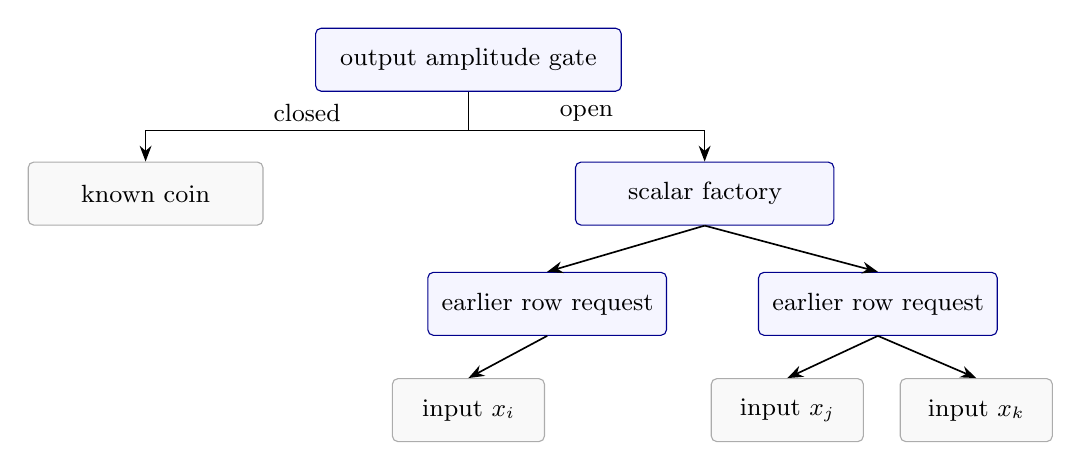
\begin{tikzpicture}[
 >=Stealth,font=\small,
 work/.style={draw=blue!55!black,fill=blue!4,rounded corners=2pt,
              minimum height=8mm,align=center,inner sep=4pt},
 terminal/.style={draw=gray!65,fill=gray!5,rounded corners=2pt,
                  minimum height=8mm,align=center,inner sep=4pt},
 edge/.style={->,semithick}]
 \node[work,text width=3.6cm] (gate) at (0,0) {output amplitude gate};
 \node[terminal,text width=2.7cm] (known) at (-4.1,-1.7) {known coin};
 \node[work,text width=3.0cm] (factory) at (3.0,-1.7) {scalar factory};
 \node[work,text width=2.75cm] (left) at (1.0,-3.1) {earlier row request};
 \node[work,text width=2.75cm] (right) at (5.2,-3.1) {earlier row request};
 \node[terminal,text width=1.65cm] (x1) at (0.0,-4.45) {input $x_i$};
 \node[terminal,text width=1.65cm] (x2) at (4.05,-4.45) {input $x_j$};
 \node[terminal,text width=1.65cm] (x3) at (6.45,-4.45) {input $x_k$};
 \draw[semithick] (gate.south)--(0,-.9);
 \draw[edge] (0,-.9)--node[above,inner sep=3pt]{closed}(-4.1,-.9)--(known.north);
 \draw[edge] (0,-.9)--node[above,inner sep=3pt]{open}(3.0,-.9)--(factory.north);
 \draw[edge] (factory.south)--(left.north);
 \draw[edge] (factory.south)--(right.north);
 \draw[edge] (left.south)--(x1.north);
 \draw[edge] (right.south)--(x2.north);
 \draw[edge] (right.south)--(x3.north);
\end{tikzpicture}
\caption{One possible request tree. Only reached calls incur work.
 A factory may request a random number of earlier signs; the two children
 shown here are one realization. Each call uses fresh randomness, so
 predictable charging bounds total work. At fixed input rank, the critical
 sampler uses the composite function through a precomputed coefficient oracle.}
\label{fig:recursion}
\end{figure}


For a whole network, each child sign can itself require a factory
(Figure~\ref{fig:recursion}).
A direct product of worst-case scalar costs gives an exponential
bound even at unit row norm. The depth analysis instead maintains
an input-independent interval
\[
 h_{\ell,i}\in c_{\ell,i}+[-r_\ell,r_\ell],
\]
where the centers and outward-rounded radii are prepared from the
weights. Sampling the normalized displacement costs close to one
child as $r_\ell$ decreases. A final known mixture restores the
center and radius.

At zero bias and unit norm, the ideal radius satisfies
$r_{\ell+1}=\tanh r_\ell$, starting from $r_0=1$. The bounds
$u^{-2}+2/3\le\coth^2u\le1+u^{-2}$ give
\begin{equation}
 \frac1{\ell+1}\le r_\ell^2\le\frac3{2\ell+3}
 \label{eq:main-radius}
\end{equation}
(Lemma~\ref{lem:radius} and Figure~\ref{fig:thresholds}), so
$r_\ell^2=\Theta(1/\ell)$. Since $\sinh^2u\ge u^2+u^4/3$, also
$\coth^2u\le u^{-2}+2/3+u^2/9$. Summing this over the recursion, with
$r_i^2\le3/(2i+3)$ and $\sum_{i<\ell}1/(2i+3)\le\sqrt\ell$, gives
$r_\ell^{-2}\le1+2\ell/3+\sqrt\ell/3$, and hence $r_\ell^2\sim3/(2\ell)$.
Thus a per-layer cost $1+c r_\ell^2+O(r_\ell^4)$ accumulates
polynomially in depth. For arbitrary biases, a concave potential
charges the positions of normalized means within their intervals.
Combining the first majority vote with the bias correction yields
the exponent $35/32$. The proof of Theorem~\ref{thm:fusedcritical}
gives the constants; its largest cutoff is an asymptotic proof device.

\begin{theorem}[Critical and supercritical networks]
\label{thm:main-depth}
For row norms at most one, weight preprocessing costs
$O(Dn^2B^6)$ and storage costs $O(Dn^2B)$; exact output sampling
uses $O(B^4(D+1)^{35/32})$ expected bit operations.
With zero biases the upper bound is $O(B^4(D+1))$.
For every $D\le n/2$ on a sufficient dyadic grid, a zero-bias
network requires $\Omega(\sqrt D)$ expected input probes.

Set $D=\lceil\log_2n\rceil$ and $b=20\lceil\log_2n\rceil$.
For every fixed $s\le1$, one uniform exact sampler has
polylogarithmic expected online work under the original
$O(Dn^2\log^6n)$ preprocessing budget. For every fixed $s>1$,
the worst-case online cost is
$n^{\Theta(\min\{\log s,1\})}$, with absolute constants in the
exponent and fixed-$s$ prefactors.
\end{theorem}

Theorem~\ref{thm:upper} gives the preprocessing bounds,
Theorems~\ref{thm:fusedcritical} and~\ref{thm:zero-bias-linear}
the two upper bounds, Theorem~\ref{thm:lower} the probe bound, and
Corollary~\ref{cor:threshold} the threshold.

The supercritical statement determines the scale of the exponent.
It does not determine its leading constant. Near $s=1$, the best
full-class upper rate proved here is
$(51/16)(s-1)+O((s-1)^2)$ per layer; the lower rate is $2\log s$,
until it reaches the input-size cap. These rates leave a genuine gap.
For convex residual tanh layers with step $\alpha$, the fixed-$s>1$
polylogarithmic threshold at polynomial depth is
$\alpha D=O(\log\log n)$ (Corollary~\ref{cor:residual-loglog-depth}),
and at $s=1$ the upper bound becomes $O(B^4(1+\alpha D)^{35/32})$
(Theorem~\ref{thm:residualfused}).

Exact sampling is also separated from certified evaluation. In the
critical mean-chain family, computing the activation to error
$2^{-20\lceil\log_2n\rceil}$ requires $\Omega(n)$ probes, while the
exact sample uses polylogarithmic work
(Proposition~\ref{prop:evaluation}); we do not claim that every
individual network needs the $\Theta(Dn^2)$ operations of dense
evaluation.

\begin{figure}[t]
\centering
\begin{minipage}[t]{.41\textwidth}
\centering
\vspace{0pt}
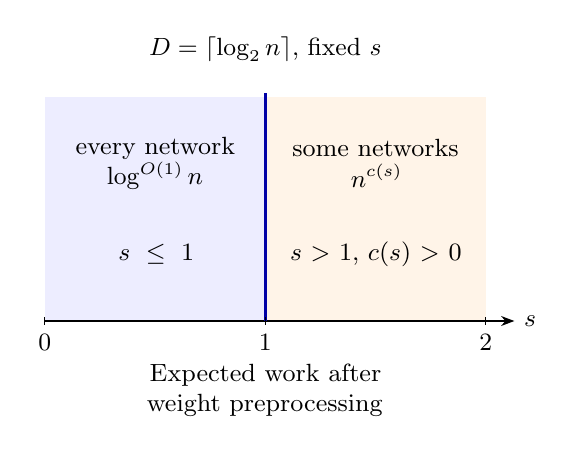
\begin{tikzpicture}[x=2.8cm,y=1cm,>=Stealth,font=\small]
 \node[align=center] at (1,3.7) {$D=\lceil\log_2 n\rceil$, fixed $s$};
 \fill[blue!7] (0,.25) rectangle (1,3.1);
 \fill[orange!9] (1,.25) rectangle (2,3.1);
 \draw[->] (0,.25)--(2.13,.25) node[right] {$s$};
 \draw[very thick,blue!65!black] (1,.25)--(1,3.15);
 \foreach \x/\lab in {0/0,1/1,2/2}
   \draw (\x,.3)--(\x,.2) node[below] {$\lab$};
 \node[align=center,text width=2.45cm] at (.5,2.25)
   {every network\\$\log^{O(1)}n$};
 \node[align=center,text width=2.45cm] at (1.5,2.25)
   {some networks\\$n^{c(s)}$};
 \node[align=center,text width=2.45cm] at (.5,1.1)
   {$s\le1$};
 \node[align=center,text width=2.45cm] at (1.5,1.1)
   {$s>1$, $c(s)>0$};
 \node[align=center,text width=5.8cm] at (1,-.63)
   {Expected work after weight preprocessing};
\end{tikzpicture}
\end{minipage}
\hfill
\begin{minipage}[t]{.56\textwidth}
\centering
\vspace{0pt}
\begin{tikzpicture}
\begin{axis}[
 width=.96\linewidth,height=4.8cm,
 xmode=log,ymode=log,log basis x=2,
 xlabel={layer index $\ell+1$},ylabel={$r_\ell^2$},
 xmin=.9,xmax=145,ymin=.007,ymax=1.2,
 xtick={1,4,16,64},xticklabels={1,4,16,64},
 ytick={1,.1,.01},yticklabels={$1$,$10^{-1}$,$10^{-2}$},
 tick label style={font=\small},label style={font=\small},
 legend columns=3,
 legend style={font=\small,draw=none,fill=none,
               at={(.5,-.3)},anchor=north,inner sep=1pt,
               column sep=2pt},
 grid=major,grid style={gray!18},
 samples=160]
 \addplot[blue!70!black,thick,domain=1:129]{3/(2*x+1)};
 \addlegendentry{upper bound}
 \addplot[orange!85!black,thick,dashed,domain=1:129]{1/x};
 \addlegendentry{lower bound}
 \addplot[black,only marks,mark=*,mark size=1.2pt]
   table[x expr=\thisrow{l}+1,y=r2,col sep=comma]{figures/radius.csv};
 \addlegendentry{recurrence}
\end{axis}
\end{tikzpicture}
\end{minipage}
\caption{The row-norm threshold and the critical radius.
 Left: $s$ bounds the absolute row sums. At logarithmic depth, the
 original preprocessing budget gives polylogarithmic sampling for
 $s\le1$; every fixed $s>1$ permits a polynomial lower-bound family.
 The leading supercritical exponents remain unmatched.
 Right: both axes are logarithmic, displaying the proved bounds
 $1/(\ell+1)\le r_\ell^2\le3/(2\ell+3)$ across the depth range.
 The black dots are numerical values of $r_0=1$,
 $r_{\ell+1}=\tanh r_\ell$; no proof uses them.}
\label{fig:thresholds}
\end{figure}


\subsection{A sharp critical law at bounded input rank}

If the first matrix has rank $r$, choose a bounded maximum-volume
basis of $r$ rows. Each basis row defines an unknown scalar mean of the input.
The subsequent signed network is a known function of these few
means. Preprocessing can therefore treat the composite function
on a fixed-dimensional box.

\Needspace{11\baselineskip}
\begin{theorem}[Critical networks with fixed first-layer rank]
\label{thm:main-bottleneck}
Fix $r\ge1$. For a zero-bias, norm-one network whose first matrix
has rank at most $r$, exact sampling uses $O_r(\sqrt{D+1})$
expected input probes and
$O_r(B^{\max\{4,r+2\}}\sqrt{D+1})$ expected bit operations. At
$D=\lceil\log_2n\rceil$ and $b=O(\log n)$, preprocessing
and storage fit $O_r(Dn^2\log^6n)$.
If $n\ge D+1$ and $b\ge\lceil\log_2(D+1)\rceil$ on the
coefficient grid $2^{-b}\mathbb Z$, the worst-case query order
is $\Theta_r(\sqrt D)$. The constants and online bit exponent
depend on the fixed rank cap.
\end{theorem}

Theorem~\ref{thm:fixed-rank-critical} proves this statement.
The output magnitude is $O(D^{-1/2})$. Open a dyadic gate of
that order and, on its open branch, sample a bounded normalized
function. The corrected scalar Bernstein operator is
\[
 T_m f=B_m\left(f-\frac{p(1-p)}{2m}f''\right),
\]
where $B_m$ averages a function over the empirical bias of $m$
coin flips. Exact degree elevation makes successive dyadic
corrections $O(m^{-2})$. In several coordinates, we telescope the
product of the corrected operators one coordinate at a time, so
coefficient work does not multiply across coordinates. Derivative
bounds through order $2r+2$ give $O_r(D)$ sources on the open gate,
hence the square-root bound. The coefficient oracle is compiled on
$O_r(D^{r/2})$ Taylor patches and batched before each dense layer by
rectangular matrix multiplication~\cite{legall2012rect}, within the
original preprocessing budget (Appendix~\ref{sec:fixed-rank-batching});
its constants may be enormous. Rare unresolved comparisons are refined
directly and paid for by their probability. For
first-layer rank at most three, after general-depth preprocessing,
a rare full-input read also gives the finite-width law
$\Theta(\min\{\sqrt D,n/\sqrt D\})$ in expected
probes when $b\ge\lceil\log_2\min\{n,D+1\}\rceil$
(Corollary~\ref{cor:rank-three-finite-input}, with the lower
bound from Theorem~\ref{thm:finitecritical}).

\paragraph{A sufficient condition without a rank bound.}
The column envelope $C_{\rm col}=\sum_j\max_i|w_{1,ij}|$ gives
a second sharp subclass and a uniform upper bound. Put
$K_{\rm col}=\max\{1,C_{\rm col}\}$.
Theorem~\ref{thm:column-envelope-critical} proves
\[
 \E Q=O(K_{\rm col}^2\sqrt{D+1}),
 \qquad \E W=O(K_{\rm col}^7\sqrt{D+1}\,B^{40})
\]
within the original preprocessing budget at logarithmic depth.
For example, a Hadamard matrix divided by its width has full rank
and column envelope one. A single weighted coordinate probe represents
an entire bounded random vector with the required mean. A corrected
empirical average and sampled fourth derivatives give the exact coin.
The large bit exponent is a conservative implementation bound.


\section{What an input lower bound measures}
\label{sec:lower-main}

Fix a network and let $f(x)$ be its output sign mean. Supply its
input coordinates independently with mean $t\in(-1,1)$, and set
$H(t)=\E_t f(X)$. An exact sampler returns a sign $Y$ with this
mean. Repeated input probes can be memoized without revealing new
information. If $Q$ is the number of distinct coordinates exposed,
the transcript score is
\[
 Z=\sum_{\text{newly exposed }i}\frac{X_i-t}{1-t^2}.
\]
The finite input population gives exact identities
\begin{equation}
 \E_t Z^2=\frac{\E_t Q}{1-t^2},\qquad
 H'(t)=\E_t(YZ).
 \label{eq:main-score}
\end{equation}
Each new input is independent of the preceding transcript.
Consequently the score increments are orthogonal martingale
differences. The output identity follows by differentiating the
finite input distribution, followed by conditioning on the transcript.
There is no assumption that the sampler's internal arithmetic has
an exponential tail.

Since $\E_tZ=0$, also $H'(t)=\E_t[(Y-H(t))Z]$, and Cauchy--Schwarz gives,
when $|H(t)|<1$,
\begin{equation}
 \E_t Q\ge
 \frac{(1-t^2)H'(t)^2}{1-H(t)^2}.
 \label{eq:main-information}
\end{equation}
A second differentiation gives the curvature bound
$|H''(t)|\le 2\E_tQ/(1-t^2)$. Lemma~\ref{lem:transcript} proves the
identities~\eqref{eq:main-score}, the bound~\eqref{eq:main-information}
as~\eqref{eq:transcript-variance}, and the curvature bound. Lemma~\ref{lem:new-finite-score} gives
the first-score identity for unknown-coin factories from a finite
first moment alone. The transcript-score method is prior work, with
classical precedents in Wolfowitz's sequential Cram\'er--Rao
inequality and Mendo's Bernoulli-factory lower
bound~\cite{wolfowitz1947,mendo2019}.

A complementary bound applies to two fixed inputs. Couple the
algorithm's random tapes on $x$ and on $x^{(i)}$, which differs
only at coordinate $i$. Until that coordinate is queried, the
transcripts agree. Therefore
\begin{equation}
 \PP_x(i\text{ is queried})
 \ge \TV(\mathcal L_x(Y),\mathcal L_{x^{(i)}}(Y)),
 \label{eq:main-coupling}
\end{equation}
as proved in Lemma~\ref{lem:attentioncoupling}. Summing this
inequality over many possible changes can force search through a
context.

Preprocessing determines when these arguments apply. A weight-only
index is identical on $x$ and $x^{(i)}$, so the coupling remains
valid. A cache index built from the context can differ before the
query starts. The coupling then gives no online lower bound.
For example, if all keys are identical, a prefill computation can
store the average value. A lower bound obtained by hiding an
exceptional value in a fresh context disappears under that
preprocessing. The indexed lower bound in Section~\ref{sec:index-main}
uses a different reduction.

\section{Attention before a cache index is available}
\label{sec:attention-main}

Attention is already an average. The unknown part is its
query-dependent sampling distribution. Suppose that $|a_j|\le A$
and that an independent sign of mean $a_j/A$ is available.
Choose a position $j$ uniformly, draw $N\sim\Pois(2A)$, and test
$N$ independent bits of bias $(1+a_j/A)/2$. Accept the position
if every test succeeds; stop at the first failure otherwise.
The acceptance probability is exactly
\begin{equation}
 \E\left(\frac{1+a_j/A}{2}\right)^N
 =\exp(a_j-A).
 \label{eq:main-poisson}
\end{equation}
Conditioning on acceptance therefore gives the attention law
$\pi_j$. A fresh value sign at the accepted position completes
the sample.

This identity does not require evaluating a score. For
$a_j=\beta\langle Qh_t,Kh_j\rangle/n$, choose a coordinate uniformly
and multiply independent query and key signs. Each score test uses
at most two predecessor requests. The stopped test count over the
whole race is at most $e^{2A}-1$ in expectation, so the complete
attention sign uses at most
\[
 2e^{2A}-1
\]
expected predecessor requests and $O(B^4e^{2A})$ auxiliary bit work
(Theorem~\ref{thm:attentionprimitive}).
The Poisson variable is generated through finite-bit procedures;
large numerical means are handled in blocks with stopping before
unused blocks are drawn.

A softmax over logits $z_k\in[-1,1]$ uses the same construction
with $A=1$. One proposal selects a token uniformly and accepts
with probability $e^{z_k-1}$. The expected proposal count is
at most $e^2$, and the expected total number of logit-sign
requests is at most $e^2-1$ (Theorem~\ref{thm:boundedsoftmaxinterface}).
Thus a bounded categorical output
adds a constant expected number of logit requests and an
address cost of order $\log V$.

\begin{theorem}[Attention with bounded scores, and its search boundary]
\label{thm:main-attention}
If all needed score radii, value radii, and recursively supplied
sign costs are bounded independently of $T$, one exact attention
output sample has no linear dependence on $T$.
The local expected factor is at most $2e^{2A}-1$ source requests.

For $\beta\ge0$, there is a one-block binary family with row norms at most $s\ge1$
and convex residual weight $\alpha$ whose optimal worst-context
probe cost satisfies
\begin{equation}
 Q^*_{\rm bin}=\Theta(1+\alpha\min\{T,e^{2\beta s^2}\}).
 \label{eq:main-binary-law}
\end{equation}
Its exact bit upper bound is
$O(B^4[1+\alpha\min\{T,e^{2\beta s^2}\}])$.
These bounds allow weight-only preprocessing.
\end{theorem}

Theorem~\ref{thm:attentionprimitive} proves the first part and
Theorem~\ref{thm:binaryattentionlaw} the second.

To see the lower mechanism, let a position contain a hidden sign
$x_j$, give it score $Ax_j$, and use the same sign as its value.
At the all-negative input, changing one position raises its
attention mass to $e^{2A}/(T-1+e^{2A})$. The final token probability
changes by a constant times this mass and $\alpha$. Summing the
coupling inequality~\eqref{eq:main-coupling} proves the lower bound.
The full proof keeps both residual sublayers and the bounded
softmax head.

Under standard scaling, $A=\sqrt n\,s^2$ in this family.
Consequently $2\sqrt n\,s^2\ge\log T$ can force
$\Omega(\alpha T)$ expected context probes. A bounded coordinate
range does not by itself give a context-length-independent
guarantee at standard scaling. When $n$ is fixed, this score bound
is also fixed; a uniform statement in growing $n$ must retain
the dependence on $A$.

Several blocks compose through their expected source counts, as in
Section~\ref{sec:tanh-main}. Shared centers can improve this product:
the score term common to every position cancels, and the uncertainty
radius shrinks through critical tanh layers.

\section{Exact sampling after prefill}
\label{sec:index-main}

\subsection{A lower bound for arbitrary fresh queries}

The randomized Orthogonal Vectors Hypothesis, abbreviated randomized
OVH, says that for every $\eta>0$ there is a constant $c>0$ such
that no bounded-error randomized algorithm solves balanced
Orthogonal Vectors on two sets of $N$ vectors in
$\{0,1\}^{c\log N}$ in time $O(N^{2-\eta})$.
Randomized SETH implies this hypothesis. We state the randomized
assumption because the sampler and the prefill algorithm may
both use randomness.

Haverbeck et al.~\cite[Theorem 4.1]{haverbeck2026attention} already
prove a constant-error attention lower bound after arbitrary
polynomial KV preprocessing; the hardness principle and the
dummy-key separation below are theirs.

\begin{theorem}[A polynomial index does not remove the general barrier]
\label{thm:main-index-hard}
Assume randomized OVH. For every fixed polynomial prefill bound
and every $\epsilon>0$, there is no uniform algorithm which,
for every static bounded cache and every fresh query, samples the
bounded-logit final token in expected time
$T^{1-\epsilon}\poly(n,B)$.
This holds at
\[
 n=O(\log^2T),\qquad \beta=\sqrt n,
\]
with row norms at most one, sign or zero cache coordinates, and
a binary output. It also holds if the returned law may have
total-variation error at most $1/64$.
\end{theorem}

Theorem~\ref{thm:indexedlowerlogtwo} proves this statement, and
Corollary~\ref{cor:indexedlogtwoblock} realizes it with a row-norm-one
block. An exact scan takes $O(TnB^4)$ expected bit work
(Lemma~\ref{lem:newcachescan}), so the conditional
lower bound matches the power of $T$ at these widths. The statement
is a fine-grained conditional barrier. It is not an unconditional
$\Omega(T)$ data-structure lower bound.

The reduction places candidate keys against dummy keys. A witness
makes the total candidate weight large; without a witness it is
small. A legal tanh layer and binary softmax preserve a constant
probability gap. Coordinate repetition and Rubinstein's
gap-Hamming reduction~\cite{rubinstein2018ann} give the stated
bounded-coordinate width, and bucketing one side of the hard instance
handles every fixed polynomial prefill budget.
Section~\ref{sec:prior-main} compares this bound with earlier
attention and kernel-density lower bounds.

\subsection{An index that accepts new keys}

Fixed-dimensional key geometry permits both cheap queries and
cheap maintenance. The next theorem assumes finite dyadic records.
Section~\ref{sec:full-decoder-main} includes their neural construction.

\begin{theorem}[Appendable fixed-rank attention]
\label{thm:main-fixed-rank}
\label{thm:main-dynamic}
Fix $r\ge1$ and dyadic coordinate bounds $K,Q_{\max}>0$. Keys belong
to $[-K,K]^n$, queries to $[-Q_{\max},Q_{\max}]^n$, and every cache prefix
has affine rank at most $r$. Records and queries have at most
$b$ bits per scalar. Let $\beta$ be nonnegative dyadic or
$\sqrt n$, and choose dyadic $\beta\le\bar\beta\le2\beta$
when $\beta>0$, and set $\bar\beta=0$ when $\beta=0$.
Queries use a nonempty cache, $T\ge1$. There is an exact index with
\[
\begin{aligned}
 \text{worst-case append work}&=O_r((n+\log(T+2))B^3),\\
 \text{stored bits}&=O_r((T+1)nB),\\
 \text{expected query work}&=O_r((n+M_T+\log(T+2))B^4),
\end{aligned}
\]
where
\[
 M_T\le\min\{T,(r+1)(5+32r\bar\beta Q_{\max}K)^r\}.
\]
A query uses fewer than $17/8$ proposals in expectation and
returns an index with the exact attention probabilities.
The result holds conditionally on every adaptive legal history.
At $\beta=0$, uniform index sampling suffices.
\end{theorem}

Theorem~\ref{thm:dynamicfixedrank} proves this statement.

At standard scaling and fixed $r,K,Q_{\max}$, the query bound is
$O_r((n+n^{r/2}+\log(T+2))B^4)$. Appending a record never
scans its predecessors. These bounds settle the maintenance
question in the fixed-rank, bounded-coordinate regime.

To construct the index, choose a rational coordinate chart whose
reconstruction coefficients have magnitude at most two. A row swap
that increases a coefficient beyond two doubles a nonzero minor, so
integer determinant bounds limit the number of swaps
(Lemma~\ref{lem:dynamicchart}).
On a grid where scores within a cell differ by at most $1/4$ for every
legal query, cell representatives give a constant-factor rejection
envelope (Lemma~\ref{lem:dynamiccellenvelope}). When an append
increases the rank, we keep the earlier charts and their records and
start a new chart for future records. Rank increases at most $r$
times, so a query combines at most $r+1$ chart indices and a large
degenerate prefill causes no later migration. The keys may also lie
within a small certified distance of a fixed subspace
(Corollary~\ref{cor:dynamicapproximatespace}). For rank one, an ordered
tree with blocks of sizes $1,1,2,4,\ldots$ and the classical monotone
envelope~\cite{chewi2022} give polylogarithmic context cost at every
numerical temperature (Theorem~\ref{thm:newrankone} and
Corollary~\ref{cor:dynamicrankone}).

\subsection{An implicit rank-one query and a worked example}

Reading all $n$ query coordinates is unnecessary in some regimes.
Suppose the relevant scalar projection is available through
independent coins of unknown bias $p$. A rank-one cache gives
an attention-coordinate function
\begin{equation}
 u(p)=\frac{\sum_{j=1}^T v_j e^{a_jp+c_j}}
            {\sum_{j=1}^T e^{a_jp+c_j}},
 \qquad |v_j|\le1,\quad |a_j|\le\Lambda .
 \label{eq:main-scalar-attention}
\end{equation}
The parameters have rational encodings, or the slopes and offsets
share the specified factor $1/\sqrt n$. The offsets need no magnitude bound.
The scalar corrected Bernstein factory returns a sign of mean
$u(p)/2$ in $O((1+\Lambda^2)B^4)$ expected auxiliary work and
$O(1+\Lambda^2)$ source requests. Its certified table has
polynomial prefill cost in $T$ and the numerical slope bound
$\Lambda$ (Theorem~\ref{thm:implicitrankone}). This interface
samples a value coordinate; an explicit attention index has a
different output.

For raw sign queries, combine this construction with reading the
whole query and using the explicit rank-one index. Consider dyadic
rank-one caches with keys in $[-1,1]^n$ and scalar values in $[-1,1]$.
For dyadic $\beta\ge1$ and for $\beta=\sqrt n$, the worst-cache
query law for the unit tanh and binary softmax head becomes
\begin{equation}
 Q^*_{\mathrm{rank}\,1}
   =\Theta(\min\{n,\beta^2\}).
 \label{eq:main-rankone-law}
\end{equation}
The upper bit cost is
$O((1+\min\{n,\beta^2\}+\log T)B^4)$
(Theorem~\ref{thm:rankone-worstlaw}). The implicit table
is built only when $12000\beta^2<n$, which keeps preprocessing
polynomial in $T,n,b$ even when the encoded temperature is
numerically very large.

\paragraph{Worked example.}
Let half the $T$ keys equal $\mathbf1$ and half equal
$-\mathbf1$, with corresponding values $+1$ and $-1$.
For a fresh sign query $x\in\{-1,1\}^n$, put
$M=n^{-1}\sum_i x_i$. Its attention value is exactly
$u=\tanh(\beta M)$. A unit tanh update followed by logits
$\pm\tanh u$ gives final sign mean
\[
 f(x)=\tanh(\tanh(\tanh(\beta M))).
\]
Prefill stores two groups. Appending another key from these
groups changes one group count;
the index then handles any new query from those counts. Nevertheless, the score lower bound forces
$\Omega(\min\{n,\beta^2\})$ fresh-query probes.
At $\beta=\sqrt n$ this is $\Theta(n)$, with an upper bound
$O(nB^4)$, for every even $T$. At fixed $\beta$, the expected
probe count is constant (Theorem~\ref{thm:rankonequerylaw}). This
example separates cache length from the amount of information needed
from a new query.

\subsection{A known finite query list}

A second static positive case requires no rank bound. Suppose the
permitted queries are a known list of size $M$, each specified
online by its list identifier. If all $V$ probabilities of one
candidate can be enclosed to width $2^{-t}$ in $H(B+t)^d$ bit
operations, with fixed $d\ge2$ and $H\ge V$, then
Theorem~\ref{thm:finite-query-list} gives
$O(MH[B+\log(VH+2)]^d)$ prefill work and
$O([B+\log(VH+2)]^d)$ expected work per exact sample. The table
leaves a residual mass of order $1/H$; a certified full calculation
on that branch pays for itself in expectation. Such a table is specific
to one cache; the decoder in the next section maintains one causal
evaluator as the history and the required precision change.

\section{A complete autoregressive decoder}
\label{sec:full-decoder-main}

This section states the decoder bound announced in the introduction
and the ideas of its proof. The index of Section~\ref{sec:index-main}
assumes finite records. The decoder also constructs each new key and
value with the neural model and charges that work.

Fix a dyadic embedding table with entries of magnitude at most $s$
and a causal network of the pre-norm form~\eqref{eq:main-prenorm}.
Use dyadic residual steps in $[0,1]$; convex residual mixtures with
coefficients in $[0,1]$ are also allowed. Allow an affine attention
output map and an affine vocabulary head. Parameters have at most $b$ bits,
row norms and biases are at most $s\ge1$, the temperature is
nonnegative dyadic or $\sqrt n$, and every normalization
has positive stabilizer at least $2^{-b}$. Each layer's fixed
linear key map has rank at most $r$. Its keys at all positions
must lie in one common affine space; separate rank bounds on
position-dependent maps do not imply that promise.

\begin{theorem}[Exact decoding with maintained neural keys]
\label{thm:main-decoder}
For each fixed $r$, there is a constructive polynomial $F_r$
such that a prompt of length $T_0\ge1$ can be prefilled in
\[
 T_0F_r(n,D,V,b,s,\beta,\log(T_0+2))
\]
bit operations. Every subsequent token has conditional expected
cost at most
\[
 F_r(n,D,V,b,s,\beta,\log(T+2)),
\]
given every previously sampled token history. This includes key
and value creation, insertion, random bits, and all refinements.
The output has the exact original autoregressive law.
At $\beta=\sqrt n$, with $D,V,b,s$ polynomially bounded in $n$,
the per-token bound is $\poly_r(n,\log T)$.
The affine head's logit range is determined from the parameter
bounds. The polynomial degree depends on $r$.
\end{theorem}

Theorem~\ref{thm:momentdecoder} proves this statement for logits
promised to lie in $[-1,1]$, and Corollary~\ref{cor:affineheadmoment}
removes that promise for the affine head.

In a bounded chart, write a score, up to a common offset, as
$\langle t,z_j\rangle$, where $z_j\in[-1,1]^r$ and
$\|t\|_1\le H=\poly_r(n,s,\beta)$. A degree-$m$ Taylor
expansion uses $\binom{m+r}{r}$ monomials. Store their sums
and their value-weighted sums as exact integers over a common
dyadic denominator. Each new record adds to these counters.
Degree $m=O(H+p)$ yields certified attention accuracy $2^{-p}$;
the average denominator is at least $e^{-H}$, so this includes
the error of division. At $\beta=\sqrt n$, rational even and
odd degree sums keep the specified square root exact.

Attention is Lipschitz from the maximum score error to the total
probability error with constant two, independently of the number
of keys. For positive RMS stabilizers, the logarithm of the Lipschitz
constant is of order $b+\log n$. Consequently errors propagate through
the $D$ layers, with no linear factor in the number of positions.
A precision of
$p+O\bigl((D+1)[b+\log(n+s+\beta+2)]+\log(D+V+2)\bigr)$
suffices.
Rounding the normalized stream before its exact key-map product
preserves the promised rank. This detail prevents a finite
approximation from silently changing the structural hypothesis.

Routine precision is a sufficiently large multiple of $\log T$.
If a uniform draw is too close to a categorical boundary, replay
the actual token history at higher precision until the sample is
certified. An unresolved precision-$p$ comparison has probability
at most $4V2^{-p}$. Choosing routine error of order $T^{-3}/V$
pays for a complete replay on that rare branch. A second routine
index replays two old tokens after each append and catches up
before the current precision expires. Ordinary maintenance uses
at most three deterministic token evaluations per step.
Figure~\ref{fig:decoder-overview} shows this maintenance loop.

For a basic tanh model with an affine head that is fixed in all
parameters, the key ranks are fixed even when the key matrices have
full rank. The explicit implementation gives
$O_{\rm model}(\log^{2r+12}(T+2))$ expected work per token, with
model-dependent constants that can be enormous
(Corollary~\ref{cor:fixedmodelcontext}).
Fixed coordinate-pair positional rotations also admit a
$\log^{O_{\rm model}(1)}T$ bound: certified trigonometric
evaluation costs polynomial time in precision and $\log T$
(Corollary~\ref{cor:fixedpositionalrotation}). The same
finite-evaluation argument covers specified GELU and SwiGLU updates
using their polynomial range and Lipschitz bounds on bounded
normalized inputs (Corollary~\ref{cor:momentgeluswiglu}).

\section{Normalization and additive residuals}
\label{sec:additive-main}

\subsection{Two exact interfaces for RMS normalization}

Let $a\in[-R,R]^n$, let $\varepsilon\ge0$, and consider
$\RMS_\varepsilon(a)$ from~\eqref{eq:main-rms}.
RMS normalization removes the mean-subtraction step of
LayerNorm \cite{zhang2019rmsnorm}. The Gaussian construction
below also applies to regularized LayerNorm after centering.

\begin{theorem}[Exact RMS normalization]
\label{thm:main-rms}
Suppose $R>0$, $\varepsilon\ge0$, and $\lambda>0$ are known rational
parameters, and $\lambda$ certifies
$\varepsilon+n^{-1}\sum_j a_j^2\ge\lambda$ on every allowed input,
and put $\kappa=\max\{1,R^2/\lambda\}$. Independent signs of mean
$a_j/R$ suffice for an exact sign interface for
$\RMS_\varepsilon(a)_i$ at radius $2R/\sqrt\lambda$, using at most
$O(1+\kappa^2)$ expected source requests and
$O(\kappa^2B^4)$ auxiliary bit operations.

If $\varepsilon>0$, a second construction has radius $4\sqrt n$.
With $\kappa_\varepsilon=R^2/\varepsilon$, it uses at most
$1+n\kappa_\varepsilon$ expected source requests and
$O(n(1+\kappa_\varepsilon)B^4)$ auxiliary work.
\end{theorem}

Theorems~\ref{thm:rmsfloor} and~\ref{thm:gaussianrms} prove the bounds
for the two constructions. The first samples a coordinate and two independent
signs, whose disagreement probability represents
$(1-n^{-1}\sum_j(a_j/R)^2)/2$. A linear Bernoulli factory uses
the certified floor, and a negative-binomial expansion supplies
the inverse square root. The second projects onto a random Gaussian
direction; an error-function factory gives an arcsine transform of
$a_i/\sqrt{\|a\|_2^2+n\varepsilon}$, which a signed sine-series
mixture inverts. Applied to signs of mean $(a_i-\bar a)/(2R)$, with
$\bar a=n^{-1}\sum_j a_j$, it also gives regularized LayerNorm at
radius $4\sqrt n$ (Corollary~\ref{cor:gelulayernorm}).
Error-function factories and trigonometric stochastic constructions
have prior precedents \cite{flajolet2011buffon,gaines1969}, and
Gaussian sign identities and inverse-power corrections occur
in rounding theory \cite{braverman2011grothendieck}.
The contribution here is the explicit normalization interface,
its source and bit bounds, and its use inside the network
recurrence.

A positive stabilizer alone gives no uniform small cost.
For the scalar family
\[
 f_{\kappa,A}(z)=\frac{z}{A\sqrt{\kappa^{-1}+z^2}},
 \qquad A\ge1,
\]
the optimal uniform source count obeys
\begin{equation}
 \frac{\sqrt\kappa+\kappa}{8A}
 \le Q^*(\kappa,A)
 \le \frac{1+2\kappa}{A\sqrt{1+\kappa^{-1}}}
 \le \frac{3(\sqrt\kappa+\kappa)}A
 \label{eq:main-scalar-rms-law}
\end{equation}
(Theorem~\ref{thm:scalar-rms-amplitude}). At fixed $A$ and large
$\kappa$ the cost is of order $\kappa$, and increasing the radius to
order $\sqrt\kappa$ reduces it to order $\sqrt\kappa$. The lower bound
needs only a uniform first moment.

\subsection{The additive recursion}

Consider sublayers
\[
 H_j=H_{j-1}+F_j(H_{j-1}),\qquad |H_0|\le1,
 \qquad |F_j(H)_{t,i}|\le U_j,
\]
where $U_j\ge0$ is a known bound. Set
$R_j=1+\sum_{k\le j}U_k$. The quantity $B$ includes the full
finite encodings of these radius prefixes.
Suppose an exact sign of mean $F_j(H)_{t,i}/U_j$ uses at most
$m_j$ expected predecessor signs of mean
$H_{t',i'}/R_{j-1}$ and at most $C_0B^4L_j$ expected local bit
work. Zero updates are omitted. These are uniform conditional
bounds, so they remain valid when the factory is called
adaptively.

\begin{theorem}[An additive cost product]
\label{thm:main-additive}
Put
\[
 P_j=\prod_{k=1}^j\left(1+\frac{U_km_k}{R_{k-1}}\right).
\]
There is an exact sampler for $H_{J,t,i}/R_J$ with at most
$P_J/R_J$ expected input leaves and at most
\begin{equation}
 C_0B^4\frac{P_J}{R_J}
 \left(2+\sum_{j=1}^J\frac{U_j(1+L_j)}{P_j}\right)
 \label{eq:main-additive-cost}
\end{equation}
expected bit work.
If $m_j\le m$ for $m\ge1$ and $L_j\le L$, these bounds become
$R_J^{m-1}$ leaves and
\[
 C_0B^4(2+L)(1+\log R_J)R_J^{m-1}
\]
bit operations.
\end{theorem}

Theorem~\ref{thm:pn-abstract} proves this statement.
To sample $H_j/R_j$, choose the input contribution with probability
$1/R_j$ or update $k\le j$ with probability $U_k/R_j$. A prefix table
makes this choice directly, so the algorithm never traverses a long
sequence of identity branches; an update's children restart the
procedure at an earlier level. A linear recurrence for the bit work
and the inequality $\sum_jU_j/R_j\le\log R_J$ show that auxiliary
arithmetic adds only a logarithm in the residual radius.

\subsection{Pre-norm attention and feed-forward updates}

Consider the pre-norm blocks~\eqref{eq:main-prenorm}.
A \emph{relative energy certificate} with constant $\gamma>0$
asserts, at every requested normalization and for every allowed
input and position,
\begin{equation}
 \varepsilon_j+\frac1n\sum_i H_{j-1,t,i}^2
       \ge \gamma R_{j-1}^2 .
 \label{eq:main-relative-floor}
\end{equation}
This is an additional hypothesis on the network and its allowed
inputs. It does not follow from a fixed stabilizer: with stabilizer
three, networks of logarithmic depth can force linear query cost
(Theorem~\ref{thm:pn-absolute-lower} and
Corollary~\ref{cor:pn-fresh-query}).

With the power of two $G\in[2/\sqrt\gamma,4/\sqrt\gamma)$ and
$K_\gamma=1+228\max\{1,\gamma^{-2}\}$ of Theorem~\ref{thm:pn-relative},
set
\begin{equation}
 E=e^{2|\beta|s^2G^2},\quad \rho=sG,\quad
 m=\max\{1,(2E-1)K_\gamma,\,2\rho(1+\rho)K_\gamma\}.
 \label{eq:main-prenorm-m}
\end{equation}
These constants bound the number of predecessor requests for
normalized attention and tanh updates. Like $m$, the local
arithmetic factor $L$ of that theorem depends only on $\gamma,s,\beta$.
The unscaled update radii are $sG$ and $1$, and a step size
multiplies an update's radius without changing its sign factory.
Theorem~\ref{thm:main-additive} then gives polynomial dependence
on $1+\tau$, where $\tau$ is total step size, and only address
dependence on $T$ (Corollary~\ref{cor:pn-stepsizes}). For a common
step $\alpha$ and $D$ blocks, one may use $R=1+\alpha D(sG+1)$.
A final RMSNorm satisfying the same relative certificate,
followed by a bounded affine softmax head, adds a constant
factor when its row norm is fixed (Theorem~\ref{thm:pn-relative}).
A readout of the unnormalized stream costs at most a further
factor $R^2$ (Theorem~\ref{thm:quadraticscaledhead}).

The polynomial scale is necessary in a uniform theorem. There are
tanh families with a full-input relative certificate and a fixed
bounded readout that require
\begin{equation}
 \Omega_s(\min\{(1+\tau)^{2(s-1)},n\})
 \label{eq:main-prenorm-lower}
\end{equation}
probes for every fixed legal gain $s>1$. This holds for arbitrary
prescribed dyadic steps in $[0,1]$, with $\tau$ their sum
(Theorem~\ref{thm:pn-normalized-gain}, whose exponent is larger, and
Corollary~\ref{cor:pn-scheduled-lower}). Thus a
polylogarithmic accumulated step size is sufficient and necessary
for a uniform polylogarithmic guarantee in these fixed-parameter
classes (Corollary~\ref{cor:pn-effective-threshold}). Convex
supercritical residuals instead have the $\log\log n$ step-mass
scale. The next theorem sharpens the additive exponent for one
explicit family.

\begin{theorem}[A sharp additive family]
\label{thm:main-carrier}
Put $c=\tanh1$ and fix a legal dyadic $s>c/\sqrt2$.
For $n\ge4$, let $N$ be the largest power of two at most $n/2$
and put $\eta=N/n$. For prescribed dyadic steps
$a_0,\ldots,a_{D-1}\in[0,1]$, write
\[
 R_j=1+\sum_{k<j}a_k,\quad R=R_D,\qquad
 \nu_\eta=\frac{s}{c\sqrt\eta}-1.
\]
There is an explicit additive tanh family with stabilizer $3$,
row norms at most $s$, and a fixed bounded binary head whose
optimal worst-input query cost is
\[
 \Theta_s(\min\{R^{2\nu_\eta},n\}).
\]
After $O_s((D+1)n^2B^6)$ weight preprocessing, exact sampling
uses $O_s(B^4\min\{R^{2\nu_\eta},n\})$ expected bit operations.
The entire input sign cube satisfies a relative energy floor
stronger than $R_j^2/12$.
\end{theorem}

Theorem~\ref{thm:pn-family-query-law} proves the query law and
Theorem~\ref{thm:pn-family-bit-law} the bit bound.
One group carries the unknown feature mean. An equal-sized group
moves deterministically at speed $c$, driven by a bias of $-1$.
After division by the residual radius, the feature gain approaches
$s/(c\sqrt\eta)$, and the transcript score gives the lower bound. For
the upper bound, two unknown means and one observed sign determine
the head, and a Taylor oracle on a complex neighborhood of radius
proportional to $R^{-\nu_\eta}$ supplies its corrected Bernstein
factory. Rounding is amplified only through factors
$1+O_s(a_j/R_{j+1})$, so the required precision grows logarithmically
in depth. The full additive class may have a different worst-case
exponent.

The additive product also covers common feed-forward activations.
Write $\GELU(v)=v\Phi(v)$ and
$\operatorname{SwiGLU}(u,v)=u\,v\,\sigma(v)$, where $\Phi$ is
the standard normal distribution function and
$\sigma(v)=(1+e^{-v})^{-1}$. For bounded affine inputs,
error-function, product, and logistic factories give exact interfaces
with polynomial source cost in their radius
(Lemma~\ref{lem:gelu-swiglu}). For every fixed legal dyadic gain
$s\ge2$, affine GELU and SwiGLU lower constructions with an explicit
relative floor and a final RMSNorm also
satisfy~\eqref{eq:main-prenorm-lower}
(Theorem~\ref{thm:real-ffn-lower} and
Corollary~\ref{cor:real-ffn-scheduled}). The identities
$\GELU(v)-\GELU(-v)=v$ and $\SiLU(v)-\SiLU(-v)=v$, where
$\SiLU(v)=v\sigma(v)$, embed the required linear amplification using
three hidden units.

The relative-floor product gives a sufficient condition for an
architecture. Its constants can be large when row norms grow or
the floor is small. In particular, the score factor in
\eqref{eq:main-prenorm-m} grows exponentially in $\sqrt n$ at
standard scaling. The decoder of Section~\ref{sec:full-decoder-main}
instead uses the prefilled cache and charges full width-dependent
arithmetic at one position, while controlling its dependence on
context length.

\section{Quantities to check on a model}
\label{sec:checkpoint}

The positive results give sufficient conditions that can be checked
against a specified model. Their current dependence on rank is severe.
The maintained decoder is polynomial in width when its rank bound is
fixed independently of width; both its feature count and the polynomial
degree grow with that rank. These bounds currently supply no useful
speed prediction at large key ranks.

For this section, $n$ is residual width, $d$ is one head's key
dimension, and $a$ is its value dimension. Scores are
$\beta\langle q,k_j\rangle/d$, with $\beta=\sqrt d$ at standard
scaling. RMSNorm still averages over $n$ coordinates.
If its learned gain is $g$, use the effective following matrix
$W^{\rm eff}=W\operatorname{diag}(g)$. Its row budgets are
$s_i=\sum_j|W_{ij}g_j|$.
These conventions match the inside-root stabilizer, learned gain,
and head-dimension scaling of the reference implementation
\cite{llama3reference2026}. Corollary~\ref{cor:checkpoint-rectangular}
proves the rectangular-dimension extension used here.
Table~\ref{tab:checkpoint-quantities} lists the quantities to record.

\begin{table}[t]
\centering\small
\begin{tabularx}{\textwidth}{@{}>{\raggedright\arraybackslash}p{0.18\textwidth}YY@{}}
\toprule
Quantity & What to record & Where it enters\\
\midrule
Affine key rank $r$ &
An exact common containing space over allowed positions and histories;
the full effective key matrix includes all learned updates. &
Cell count $(5+O(r\beta Q_{\max}K))^r$; moment count
$\binom{m+r}{r}$.\\
Score and coordinate ranges &
Certified query/key bounds $Q_{\max},K$, value bound $U$, and score radius.
Record empirical extrema separately. &
The unindexed source factor is $2e^{2A_{\rm coin}}-1$;
the moment degree uses the chart bound $H$.\\
Row budgets &
Effective absolute row sums, biases, and weighted radii
$\rho_i=\sum_j|W_{ij}|R_j$. &
A tanh row with $|b_i|\le1$ uses at most
$2\rho_i(1+\rho_i)$ predecessor requests
(Corollary~\ref{cor:comptanhrow}).\\
Normalization floor &
The inside-root $\varepsilon$, input radius $R_{j-1}$, and a
certificate $\lambda_j\le\varepsilon_j+\|H_{j-1}\|_2^2/n$. &
$\kappa_j=\max\{1,R_{j-1}^2/\lambda_j\}$ for the floor factory;
$(1+\sqrt n)/\sqrt{\lambda_j}$ in the precision guard.\\
\bottomrule
\end{tabularx}
\caption{Quantities to record for a model and where they enter the bounds.}
\label{tab:checkpoint-quantities}
\end{table}

\paragraph{Rank and an appendable cache.}
Without positional transforms, $b_K+\operatorname{image}(W_K^{\rm eff})$
is a common key space. With rotations, the containing space must
include every rotated image and the differences of rotated biases.
Separate ranks of the transformed matrices do not certify its dimension.
Even a rank-one unrotated key image can acquire a full common span
(Proposition~\ref{prop:checkpoint-rotary-span}). The unrotated score
rank $\operatorname{rank}[(W_Q^{\rm eff})^TW_K^{\rm eff};
b_Q^TW_K^{\rm eff}]$ can sometimes replace the key rank
(Corollary~\ref{cor:checkpoint-score-rank}).

\paragraph{Formulas to evaluate.}
For supplied finite records with $M_T$ occupied index cells, the index
of Theorem~\ref{thm:main-fixed-rank} has append work
$O_r((d+a+\log(T+2))B^3)$ and query work
$O_r((d+M_T+\log(T+2))B^4)$, with
$M_T\le\min\{T,(r+1)(5+32r\bar\beta Q_{\max}K)^r\}$.
For the moment decoder with a chart bound $H$
(Appendix~\ref{app:checkpoint}) and attention precision $p$, one valid
degree and its exact feature count are $m=\lceil8(p+3H+7)\rceil$ and
$N_m=\binom{m+r}{r}$, with $(a+1)N_m$ integer counters per head and
precision index. At illustrative degree $m=256$, $N_m$ is
$2{,}862{,}209$ for rank three and exceeds $5\cdot10^{14}$ for rank
eight. For additive updates with radius increments $u_j$ (including
step sizes), source bounds $m_j$, local arithmetic factors $L_j$, an
initial radius $R_0$, $R_j=R_0+\sum_{k\le j}u_k$, and
$P_j=\prod_{k\le j}(1+u_km_k/R_{k-1})$,
Corollary~\ref{cor:checkpoint-initial-radius} gives
\[
 W_{\rm add}\le C_0B^4\frac{P_J}{R_J}
 \left(2R_0+\sum_{j=1}^J\frac{u_j(1+L_j)}{P_j}\right).
\]
Appendix~\ref{app:checkpoint} also defines the coin radius
$A_{\rm coin}$, gives the stage-by-stage precision guard
(Lemma~\ref{lem:checkpoint-precision}), and treats floors that cover
only some histories. For the critical tanh subclasses, the exact
first-layer rank and the column envelope enter
Theorems~\ref{thm:main-bottleneck} and~\ref{thm:column-envelope-critical}.

\paragraph{Interpreting measurements.}
Exact weight ranks and row budgets can be certified from the stored
parameters. A score maximum or energy minimum measured on selected
texts describes those texts. A universal claim requires a bound for
all allowed histories, or a certificate checked as records enter the
cache. Verification that reads the current context is charged to
online work. The accompanying worksheet reports construction sizes
and symbolic bit-work bounds. Timing, energy, and speedup require
an implementation and calibration at the same target law.

\section{Relation to attention approximation and prior factories}
\label{sec:prior-main}

A runtime comparison must match the output and preprocessing:
an approximate attention vector, an attention index, and a final
token impose different requirements.

KDEformer and HyperAttention give operator-norm approximations of the
attention product that hold with high probability
\cite{kdeformer2023,hyperattention2023}. Such a guarantee supplies no
certified interval for every output probability on every random run.
MagicPIG samples through a prefill-built locality-sensitive hash index
\cite{magicpig2024}; its implemented self-normalized estimate is
generally biased. Appendix~\ref{app:related} states these three
guarantees with their parameters. Randomly perturbed nearest-neighbor
methods give exact categorical samples when a valid top-$k$ oracle is
available \cite{mussmann2017}, and approximate retrieval then needs
additional certification or an error allowance. Smooth-kernel data
structures, including the quasi-Monte Carlo construction of Charikar,
Kapralov, and Waingarten \cite{charikar2024qmc}, offer another positive
route for their specified kernel class. Their smoothness condition does
not include the Gaussian kernel at arbitrary scale. These results therefore do not remove the
constant-gap indexed lower bound proved here.

Alman and Song's earlier high-precision theorem does not by itself
give the constant-gap sampling conclusion of
Theorem~\ref{thm:main-index-hard}. They study approximation of a
complete attention matrix-vector computation, with dimension, entry
bounds, and inverse-polynomial accuracy linked together
\cite{alman2023attention}. Kernel-density lower bounds also depend on
the batch model and the requested accuracy
\cite{aggarwal2022polynomial,alman2024kde}. Estimating an
inverse-polynomial probability gap by repeated samples can erase a
desired exponent saving; the constant final-token gap avoids that
loss.

Maintaining feature sums for causal attention is established work.
Katharopoulos et al.~\cite{katharopoulos2020linear} give recurrent
prefix states for feature attention. Heinsen and
Kozachkov~\cite{heinsen2026taylor} give the Taylor monomials,
feature count, and accumulated states at arbitrary truncation
order. Our decoder uses those representations with certified
error, rank-preserving rounding, and a precision schedule that
supports the exact original law through all layers.
Exact decisions from finite probability approximations also have
prior constructions. Han and Hoshi~\cite{han1997interval} study interval sampling, and
Brassard, Devroye, and Gravel \cite{brassard2019remote} give floored
rejection envelopes and geometric refinement tails. The decoder
combines these principles with a causal neural evaluator and
background replay to prove a complete finite-bit maintenance bound.
Dynamic attention maintenance~\cite{vandenbrand2024dynamic} and
dynamic KDE~\cite{liang2025dynamic} support entry or point updates
with numeric outputs, which differ from an appended neural record
followed by one exact categorical sample.

Stochastic computing represents values by event probabilities
\cite{gaines1967,gaines1969,browncard2001}. Bernoulli-factory theory
supplies analytic constructions, positive series, multivariate
races, and composition principles
\cite{nacuperes2005,holtz2011,mendo2019,dughmi2017,morina2022}.
We attribute these tools where they enter and make no novelty claim
for scalar factory representations. Koskela, Karvonen,
{\L}atuszy{\'n}ski, and Span{\`o} \cite{koskela2026debiased} give a
scalar debiased Bernoulli construction based on smooth Bernstein
approximants. Its outcome-independent sample count is useful for
composition, but does not supply the dense multivariate coefficient
oracle needed by the unrestricted critical problem. Randomized
telescoping and antithetic empirical means are also established
tools \cite{rheeglynn2015,blanchetglynn2015,blanchetchenglynn2015}.
The column-envelope theorem makes its correction estimates bounded on
every branch. Its common derivative majorants, exact quadratic and
quartic tilts, and retained observations then give a sign with the
required law and the stated input cost.

\section{Scope, remaining questions, and evidence}
\label{sec:status}

\subsection{What follows for decoding}

Before prefill, standard score scaling can force linear positional
search. After prefill, fixed-rank neural key maps with a positive
normalization stabilizer give $\poly_r(n,\log T)$ conditional expected
work per token. The OVH obstruction concerns ranks and widths that
grow with the context. Pre-norm additive residuals, RMSNorm, and
SwiGLU occur in widely used
architectures~\cite{touvron2023llama2,zhang2019rmsnorm,shazeer2020glu},
but no theorem here establishes favorable rank or numerical constants
for a trained checkpoint. Section~\ref{sec:checkpoint} lists the
quantities to certify on a model and shows how fast the moment
dimension grows with rank.

\subsection{Open problems}

\paragraph{Main open problem: the unrestricted critical exponent.}
For zero-bias networks with every row norm at most one, the worst-case
query gap remains $\Omega(\sqrt D)$ versus $O(D)$. Does an exact
sampler use $O(\sqrt{D+1})$ expected input probes at arbitrary rank,
under the same weight preprocessing budget and with polylogarithmic
bit overhead? Even $\sqrt{D+1}\log^{O(1)}(D+2)$ probes would close
the depth exponent. No factor $\log^{O(1)}n$ is hidden in this query
claim: at logarithmic depth such a factor could absorb the whole gap.
The fixed-rank theorem has constants and a bit exponent that depend
on the rank, and the column envelope $\sum_j\max_i|w_{1,ij}|$ may be
$n$, so these two certificates leave the general critical exponent
unsettled.

The final analysis sharpens the limitations of two proof routes.
The integer stopped-score obstruction also holds for bounded real
estimators, so delayed Bernoulli rounding does not reduce the leading
local amplification cost (Corollary~\ref{cor:new-integer-score}).
A common derivative majorant shows that the
sum of one-coordinate coupling witnesses is at most one. Even grouped,
matrix-valued second-order score witnesses are at most $\sqrt{6D}$
(Propositions~\ref{prop:critical-hessian-majorant}
and~\ref{prop:critical-matrix-score}). These are ceilings on the stated
lower-bound methods. They neither prove a faster global sampler nor
rule out a stronger lower bound by another method.
Near unit row norm, the supercritical gap remains between
$2\log s$ and $(51/16)(s-1)+O((s-1)^2)$ per layer.

The full relative-floor class has an open additive exponent,
as does the carrier family's boundary $\nu_\eta=0$. A general instance
law also faces computational obstacles. Let $Q^*(W)$ be the optimal
worst-input expected number of distinct probes for a network $W$.
At fixed $s>1$, a deterministic polynomial-time algorithm that
approximates $1+Q^*(W)$ within a polylogarithmic factor on width-$n$
networks of depth $\lceil\log_2n\rceil$ with row norms at most $s$
and precision $b=20\lceil\log_2n\rceil$ would imply
$\mathrm P=\mathrm{NP}$. A randomized one that succeeds with
probability at least $2/3$ would imply
$\mathrm{NP}\subseteq\mathrm{BPP}$ (Theorem~\ref{thm:instance-hardness}).

For attention, useful remaining questions concern deletions,
weaker geometric promises, and algorithms whose rank dependence
is useful at model dimensions. Sharp normalization laws under input-dependent energy certificates
also remain open.

\subsection{Proofs, numerical checks, and Lean}

The appendices prove the theorem claims and identify imported
results and conditional hypotheses. The source includes numerical
and exact-arithmetic checks of coefficient identities, degree
elevation, score embeddings, and residual recurrences. These finite
checks provide supplementary evidence. No sampler benchmark or
trained-model evaluation was performed.

A Lean~4 formalization with Mathlib in the repository
\url{https://github.com/SamMausberg/exact-sampling-networks} checks many
of the probability laws, exactness identities and inequalities of the proofs,
using only the standard axioms (Appendix~\ref{app:lean}).


\paragraph{AI disclosure.}
GPT-6 Astra Pro and Claude models assisted with the mathematical proofs
and the Lean formalization.

\label{page:main-end}
\clearpage
\bibliographystyle{plain}
\bibliography{references}
\clearpage
\appendix
\renewcommand{\baselinestretch}{1}\small
\section*{Guide to the proofs}
\addcontentsline{toc}{section}{Guide to the proofs}

The scalar factories establish exact local laws. Radius and potential
bounds control their composition. Finite transcript identities give
input lower bounds. The attention appendix separates a fresh context,
an explicit cache, and a maintained neural decoder. Normalization
then supplies the additive product and its sharp carrier example.
Each formal proof begins with its main idea.

Neural biases are $b_{\ell,i}$; the unindexed $b$ bounds their
encoding length. The scalar factory uses $c_{\ell,i}$ for interval
centers. Attention temperature is $\beta$. Appendix~\ref{app:tanh}
uses the bit scale
$\mathcal B=b+\lceil\log_2(n+D+2)\rceil+16$ of~\eqref{eq:bitlength},
which is at most $B$ of~\eqref{eq:main-B}; its bounds therefore also
hold with $B$.
When a table contains $M$ groups or candidate queries, $B$ also
includes $\lceil\log_2(M+1)\rceil$. For rational residual schedules,
it includes the actual lengths of the stored radius prefixes.
A common dyadic grid keeps those lengths within the displayed
parameter and address scale; unrelated rational denominators
may require a larger $B$.

\begin{center}
\begin{tabularx}{\textwidth}{@{}p{.42\textwidth}Y@{}}
\toprule
Main result & Detailed statement and proof\\
\midrule
One tanh row & Theorem~\ref{thm:new-single-row-law}\\
Critical $35/32$ exponent & Theorem~\ref{thm:fusedcritical}\\
Zero-bias linear upper & Theorem~\ref{thm:zero-bias-linear}\\
Query lower bounds and the norm threshold & Theorem~\ref{thm:lower}; Corollaries~\ref{cor:threshold} and~\ref{cor:window}\\
Every fixed first-layer rank & Theorem~\ref{thm:fixed-rank-critical}; elementary low-rank implementations in Theorems~\ref{thm:rank-two-critical} and~\ref{thm:rank-three-critical}\\
Bounded first-layer column envelope & Theorem~\ref{thm:column-envelope-critical}; arbitrary algebraic rank\\
Convex residual scale & Theorem~\ref{thm:residualfused} and Corollary~\ref{cor:residual-loglog-depth}\\
Attention race and positional search & Theorems~\ref{thm:attentionprimitive} and~\ref{thm:binaryattentionlaw}\\
Indexed lower bound at standard scaling & Theorem~\ref{thm:indexedlowerlogtwo} and Corollary~\ref{cor:indexedlogtwoblock}\\
Appendable affine-rank index & Theorem~\ref{thm:dynamicfixedrank}\\
Full exact decoder & Theorem~\ref{thm:momentdecoder} and Corollary~\ref{cor:affineheadmoment}\\
Checkpoint certificates and dimensions & Appendix~\ref{app:checkpoint}\\
Limits of second-order score bounds & Propositions~\ref{prop:critical-hessian-majorant} and~\ref{prop:critical-matrix-score}\\
Integer stopped-score obstruction & Corollary~\ref{cor:new-integer-score}\\
Fixed model and positional rotations & Corollaries~\ref{cor:fixedmodelcontext} and~\ref{cor:fixedpositionalrotation}\\
Implicit rank-one query & Theorem~\ref{thm:implicitrankone}\\
Worst-case rank-one query law & Theorem~\ref{thm:rankone-worstlaw}\\
Finite candidate list & Theorem~\ref{thm:finite-query-list}\\
RMS normalization & Theorems~\ref{thm:rmsfloor} and~\ref{thm:gaussianrms}\\
Scalar RMS law at a fixed amplitude & Theorem~\ref{thm:scalar-rms-amplitude}\\
Additive product & Theorem~\ref{thm:pn-abstract}\\
Sharp carrier-family cost & Theorems~\ref{thm:pn-family-query-law} and~\ref{thm:pn-family-bit-law}\\
Relative-floor lower families & Theorem~\ref{thm:pn-normalized-gain}; Corollary~\ref{cor:pn-scheduled-lower}\\
GELU and SwiGLU lower families & Theorem~\ref{thm:real-ffn-lower} and Corollary~\ref{cor:real-ffn-scheduled}\\
Instance complexity & Appendix~\ref{app:instance}\\
\bottomrule
\end{tabularx}
\end{center}

A known scalar coin always denotes finite certified computation.
An unknown-mean coin denotes a supplied independent source interface.
The proofs below do not depend on the Lean formalization described
in Appendix~\ref{app:lean}.

\section{Tanh networks: scalar factories, depth, and lower bounds}\label{app:tanh}
% Exact tanh sampling: complete scalar, recursive, and lower-bound proofs.
\subsection{The tanh network model and quantitative bounds}\label{app:tanhmodel}
Let \(n\ge2\), \(D\ge1\), and \(b\ge1\). A network has activations
\begin{equation}\label{eq:network}
h_{0,j}=x_j\in\{-1,1\},\qquad
h_{\ell,i}=\tanh\!\left(b_{\ell,i}
+\sum_{j=1}^n w_{\ell,ij}h_{\ell-1,j}\right),
\quad 1\le\ell\le D.
\end{equation}
All parameters are multiples of \(2^{-b}\), and
\[
|b_{\ell,i}|\le1,\qquad
S:=\max_{\ell,i}\sum_j|w_{\ell,ij}|\le s.
\]
The exact row norm \(S\) is computed from the weights. The target
bit has probability \((1+h_{D,1}(x))/2\).

Preprocessing, probes, and online work are charged as in
Section~\ref{sec:models}, including every precision refinement.
A \emph{recursive call} is an invocation of the
normalized sampler for a neuron or input, including a repeated
invocation of the same coordinate. The root is counted as well.
Write
\begin{equation}\label{eq:bitlength}
\bits=b+\lceil\log_2(n+D+2)\rceil+16.
\end{equation}
This is at most the bit scale \(B\) of \eqref{eq:main-B}, so every
bound stated here with \(\bits\) also holds with \(B\). A plain \(B\)
in a lemma of this appendix bounds the encoding lengths of the
parameters and addresses that the lemma uses.

\begin{theorem}[Exact sampling upper bound]\label{thm:upper}
One uniform algorithm samples the target exactly for every network
with \(S\le2\), and terminates almost surely. Deterministic preprocessing
uses \(O(Dn^2\bits^6)\) bit operations and \(O(Dn^2\bits)\) stored bits.
Uniformly over all contexts, with \(\delta=(S-1)_+\),
\begin{equation}\label{eq:maincall}
\E N_{\rm calls}\le80(D+1)^2e^{51\delta D}.
\end{equation}
Expected online bit work is
\begin{equation}\label{eq:mainbit}
O\!\left(\bits^4(D+1)^2e^{51\delta D}\right).
\end{equation}
The constants in these \(O\)-bounds are absolute.
\end{theorem}

The explicit power \(2\) in \eqref{eq:maincall} counts recursive
calls. Equation \eqref{eq:mainbit} also charges the manipulation of
finite parameters and refinable scalar probabilities. A stable
fixed-precision coefficient recurrence proves the fourth-power
overhead in Section~\ref{sec:fixedprecision}.
For \(S\le1\), Theorem~\ref{thm:fusedcritical} lowers the power of
depth in \eqref{eq:maincall} and \eqref{eq:mainbit} to \(35/32\),
and Theorem~\ref{thm:zero-bias-linear} gives a linear bound when all
biases are zero.

Our lower bounds hold even with unlimited preprocessing. Set
\[
m=2^{\lfloor\log_2n\rfloor},\qquad
F_{a,0}(z)=z,\qquad F_{a,d+1}(z)=\tanh(aF_{a,d}(z)).
\]
If \(a/m\) is on the parameter grid, a legal network realizes
\(F_{a,D}(m^{-1}\sum_{j=1}^m x_j)\): the first distinguished row
has weights \(a/m\), and each later distinguished row has one
incoming weight \(a\). All other neurons and all biases are zero.

\begin{theorem}[Universal query lower bounds]\label{thm:lower}
For this network and \(a>0\), every exact sampler satisfies
\begin{equation}\label{eq:lowerexact}
\sup_x\E[Q\mid x]\ge
\frac{a^{2D}}{1+(3m-2)a^{2D}H_D/m^2},
\qquad H_D=\sum_{j=0}^{D-1}a^{-2j},
\end{equation}
where \(Q\) counts distinct input probes. If \(a>1\), then
\begin{equation}\label{eq:lowersuper}
\sup_x\E[Q\mid x]\ge
\frac{a^2-1}{4a^2-1}\min\{a^{2D},m\}.
\end{equation}
At \(a=1\) and \(1\le D\le m\),
\begin{equation}\label{eq:lowercritical}
\sup_x\E[Q\mid x]\ge\frac{\sqrt D}{100}.
\end{equation}
These bounds apply to every almost surely terminating exact algorithm.
\end{theorem}

\begin{remark}[Other averaging widths]\label{rem:lower-general-m}
The proof in Section~\ref{sec:lower} uses \(m\) only through the
output \(F_{a,D}(m^{-1}\sum_{j=1}^m x_j)\) and the condition
\(D\le m\) in \eqref{eq:lowercritical}. Theorem~\ref{thm:lower}
therefore holds for every integer \(1\le m\le n\), for example every
power of two \(m\le n\), whenever \(a/m\) is on the parameter grid.
It also holds for every legal network with this output, whatever its
other weights.
\end{remark}

Specialize now to \(L=\lceil\log_2n\rceil\), \(D=L\), and \(b=20L\).
Let \(\cost_n(s)\) be the infimum of worst-network, worst-context
expected online bit work among uniform exact samplers with
\(O(Ln^2\log^6n)\) preprocessing time and storage. The norm \(s\)
is fixed as \(n\) grows.

\begin{corollary}[The norm threshold]\label{cor:threshold}
For every fixed \(0\le s\le1\), \(\cost_n(s)=\log^{O(1)}n\).
For every fixed \(s>1\),
\begin{equation}\label{eq:dichotomy}
\cost_n(s)=n^{\Theta(\min\{\log s,1\})}.
\end{equation}
Explicitly, for \(1<s\le2\),
\begin{equation}\label{eq:explicitexponents}
\Omega_s\!\left(n^{\min\{2\log_2s,1\}}\right)
\le\cost_n(s)\le
\widetilde O_s\!\left(\min\{n^2,n^{51(s-1)/\log2}\}\right).
\end{equation}
For larger fixed \(s\), \(\widetilde O_s(n^2)\) is an upper bound.
\end{corollary}

\begin{corollary}[The transition window]\label{cor:window}
Let \(s_n=1+\delta_n\), \(0\le\delta_n\le1\), with \(D=L\) and
\(b=20L\). If \(\delta_nL=O(\log L)\), the upper bound is
polylogarithmic. If \(\delta_nL/\log L\to\infty\), no polylogarithmic
expected online bound is possible. Quantitatively, if
\(\delta L\ge4\log(30L)\), then for all sufficiently large \(L\)
some legal network and context require at least \(e^{\delta L/4}\)
expected input probes.
\end{corollary}

\begin{proposition}[Separation from numerical evaluation]\label{prop:evaluation}
For the critical mean-chain network
\(F_{1,L}(m^{-1}\sum_jx_j)\), every always-correct algorithm that
returns its activation with absolute error at most \(2^{-20L}\)
must probe all \(m\ge n/2\) relevant inputs. Even an evaluator with
success probability at least \(2/3\) on every context requires
\(m/3\) probes in expectation under uniform inputs. Exact output
sampling has polylogarithmic expected online bit work.
\end{proposition}


\subsection{Intervals and the recursive sampler}\label{sec:algorithm}
\subsubsection{Dyadic centers and radii}

Choose
\begin{equation}\label{eq:precision}
P=b+4\lceil\log_2(D+1)\rceil+8,\qquad
\varepsilon=2^{-P}.
\end{equation}
Use the reference gain \(g=\max\{1,S\}\), computed exactly from the weights.
Set \(r_0=1\) and \(c_{0,j}=0\). Obtain a dyadic \(q^\ast\) with
\(|q^\ast-\tanh(gr_{\ell-1})|\le\varepsilon/16\), and set
\(r_\ell=q^\ast+5\varepsilon/2\). Then
\begin{equation}\label{eq:rounded}
\tanh(gr_{\ell-1})+2\varepsilon
\le r_\ell\le\tanh(gr_{\ell-1})+3\varepsilon.
\end{equation}
A certified approximation followed by rational rounding supplies
this choice without finding the exact floor of a transcendental
number.

For each row store
\begin{equation}\label{eq:rowdata}
\sigma=\sum_j|w_{\ell,ij}|,\qquad
a=b_{\ell,i}+\sum_jw_{\ell,ij}c_{\ell-1,j},\qquad
\rho=\sigma r_{\ell-1},
\end{equation}
together with prefix sums of the absolute integer weight numerators.
Define the mathematical endpoints, midpoint, and image radius by
\[
y_\pm=\tanh(a\pm\rho),\qquad
m=\frac{y_++y_-}{2},\qquad R=\frac{y_+-y_-}{2}.
\]
Choose a dyadic \(c_{\ell,i}\in[-1,1]\) with
\(|c_{\ell,i}-m|\le\varepsilon\). Clamping a rounded center to
\([-1,1]\) preserves its error bound.
The exact \(m,R\) are scalar functions of stored rationals.
Online refinement does not recompute the row sum.

\begin{lemma}[Interval invariant]\label{lem:interval}
For every context, \(|h_{\ell,i}-c_{\ell,i}|\le r_\ell\).
With \(t=\tanh a\), \(q=\tanh\rho\),
\begin{equation}\label{eq:midrad}
m=\frac{t(1-q^2)}{1-t^2q^2},\qquad
R=\frac{q(1-t^2)}{1-t^2q^2}\le q.
\end{equation}
\end{lemma}
\paragraph{Proof idea.}
Propagate the endpoints of each row interval through monotone tanh. The row
norm controls its width, while a small rounding allowance keeps the stored
center and radius valid at the next layer.

\begin{proof}
The preactivation differs from \(a\) by at most
\(\sum_j|w_{\ell,ij}|r_{\ell-1}=\rho\), so monotonicity puts the
output in \([y_-,y_+]\). The tanh addition formula proves
\eqref{eq:midrad}. Its denominator is positive, and
\(1-t^2\le1-t^2q^2\). Hence
\[
R+|m-c_{\ell,i}|
\le\tanh(\sigma r_{\ell-1})+\varepsilon\le r_\ell.
\]
Induction starts with \(|x_j|=1\).
\end{proof}

\subsubsection{Normalized signs and the top output}

The internal sampler \(S_{\ell,i}\) returns a sign of mean
\(v_{\ell,i}=(h_{\ell,i}-c_{\ell,i})/r_\ell\).
At layer zero it returns \(x_i\).
For a nonzero row, choose \(j\) with probability
\(|w_{\ell,ij}|/\sigma\), request a fresh \(S_{\ell-1,j}\), and
multiply by \(\sgn(w_{\ell,ij})\).
This source has mean
\[
z=\sum_j\frac{w_{\ell,ij}}{\sigma}v_{\ell-1,j},\qquad
b_{\ell,i}+\sum_jw_{\ell,ij}h_{\ell-1,j}=a+\rho z.
\]
The next two sections construct a centered factory of mean
\begin{equation}\label{eq:centered}
G=\frac{\tanh(a+\rho z)-m}{R}.
\end{equation}

Put \(\alpha=R/r_\ell\), \(\kappa=(m-c_{\ell,i})/r_\ell\).
The internal sampler chooses the centered factory with probability
\(\alpha\), and constant signs with probabilities
\begin{equation}\label{eq:internalmixture}
\PP(+1\hbox{ constant})=\frac{1-\alpha+\kappa}{2},\qquad
\PP(-1\hbox{ constant})=\frac{1-\alpha-\kappa}{2}.
\end{equation}
The interval invariant gives \(\alpha+|\kappa|\le1\).
The resulting mean is \(\alpha G+\kappa=v_{\ell,i}\).

At the top use the actual midpoint and image radius:
\begin{equation}\label{eq:topmixture}
\PP(\hbox{centered factory})=R,\quad
\PP(+1\hbox{ constant})=\frac{1-R+m}{2},\quad
\PP(-1\hbox{ constant})=\frac{1-R-m}{2}.
\end{equation}
These probabilities are valid since \(|m|+R\le1\).
The sign has mean \(h_{D,1}\); return \((1+Y)/2\).
A zero row uses its known scalar probability directly.

\subsection{A positive majority factory}\label{sec:majority}

For \(\rho>0\), let
\(G_\rho(z)=\tanh(\rho z)/\tanh\rho\).
The unit-norm construction only needs \(\rho\le2\), but the
representation also supports the large-norm extension.
If \(M_k(z)\) is the mean of majority on \(2k+1\) independent signs
of mean \(z\), differentiating its binomial sum gives
\begin{equation}\label{eq:majderivative}
M_k'(z)=C_k(1-z^2)^k,\quad
C_k=\frac{(2k+1)\binom{2k}{k}}{4^k}\ge1,\quad
M_k(0)=0,\quad M_k(1)=1.
\end{equation}

\begin{lemma}[Majority expansion]\label{lem:majority}
Write
\begin{equation}\label{eq:generating}
F_\rho(v)=\sech^2\!\bigl(\rho\sqrt{1-v}\bigr)
=\sum_{k\ge0}d_kv^k.
\end{equation}
The coefficients are nonnegative and sum to one. Moreover
\[
\pi_k=\frac{\rho}{\tanh\rho}\frac{d_k}{C_k}
\]
is a probability distribution and
\begin{equation}\label{eq:majorityexpansion}
G_\rho(z)=\sum_{k\ge0}\pi_kM_k(z),\qquad -1\le z\le1.
\end{equation}
\end{lemma}
\paragraph{Proof idea.}
The cosine product gives nonnegative coefficients for a generating function.
Integrating the derivatives of odd-majority polynomials recovers tanh;
evaluation at the endpoint proves that the mixture weights sum to one.

\begin{proof}
The cosh product \cite{dlmf} gives
\[
F_\rho(v)=\prod_{j\ge0}
 \left(\frac{1-\eta_j}{1-\eta_jv}\right)^2,\qquad
\eta_j=\frac{\lambda_j}{1+\lambda_j},\quad
\lambda_j=\frac{4\rho^2}{\pi^2(2j+1)^2}.
\]
Each factor has nonnegative coefficients. The product converges
locally uniformly before its first pole, and
\(\sum_j\eta_j/(1-\eta_j)=\sum_j\lambda_j<\infty\).
It is a probability generating function with \(F_\rho(1)=1\).
For \(z\in[0,1]\), Tonelli's theorem and
\eqref{eq:majderivative} give
\[
\sum_k\pi_kM_k(z)
=\int_0^z\frac{\rho}{\tanh\rho}F_\rho(1-u^2)\,du
=G_\rho(z).
\]
At \(z=1\), this proves \(\sum_k\pi_k=1\).
Oddness gives negative \(z\).
\end{proof}

Sample \(K\) from \(\pi\), then request signs until one sign has
occurred \(K+1\) times. This gives the full majority's output while
sometimes using fewer than \(2K+1\) signs.

\begin{lemma}[Sequential majority cost]\label{lem:arity}
Its expected source count satisfies
\begin{equation}\label{eq:sequentialarity}
A_{\rm seq}(\rho,z)\le
1+\left(1-\frac{z^2}{3}\right)\rho^2+\rho^4.
\end{equation}
\end{lemma}
\paragraph{Proof idea.}
For each odd majority, sum the probabilities that a further vote is needed.
An integral identity expresses this cost in the same nonnegative
coefficients used by the factory and gives a uniform radius bound.

\begin{proof}
The identity \(C_k^{-1}=\int_0^1(1-v^2)^k\,dv\) follows by
integration by parts. The expected full-majority cost is therefore
\[
A(\rho)=\frac{\rho}{q}\int_0^1
\left[F_\rho(1-v^2)+2(1-v^2)F_\rho'(1-v^2)\right]\,dv.
\]
Put \(g(v)=\sech^2(\rho v)\).
Integration by parts applied to \(g(v)-1=O(v^2)\) gives
\begin{equation}\label{eq:arityintegral}
A(\rho)=\frac{\rho}{q}\left(1+
\int_0^1\frac{\tanh^2(\rho v)}{v^2}\,dv\right)
\le\frac{\rho}{q}(1+\rho^2).
\end{equation}
The singularity at zero is removable.
For \(K=1\), sequential majority costs \(5/2-z^2/2\), saving
\((1+z^2)/2\) source requests. Also
\(\pi_1=(2/3)\rho^2\sech^2\rho\).
Saving only this contribution gives
\[
A_{\rm seq}\le\frac{\rho}{q}(1+\rho^2)
-\frac{1+z^2}{3}\rho^2\sech^2\rho.
\]
Use \(\sech^2\rho\ge1-\rho^2\) and
\begin{equation}\label{eq:xcothx}
u\coth u\le1+\frac{u^2}3,\qquad u>0.
\end{equation}
For the latter, \((3+u^2)\sinh u-3u\cosh u\) vanishes at zero
and has derivative \(u(u\cosh u-\sinh u)\ge0\).
Substitution proves
\[
A_{\rm seq}\le
1+\left(1-\frac{z^2}{3}\right)\rho^2
+\frac{2+z^2}{3}\rho^4,
\]
which implies the claim.
\end{proof}

\subsection{Biases and exact stopping}\label{sec:bias}

Define \(T_\theta(u)=(u+\theta)/(1+\theta u)\).
The addition formula implies
\begin{equation}\label{eq:biasidentity}
\tanh(a+\rho z)=m+R\,T_{tq}(G_\rho(z)).
\end{equation}
For \(\theta\ge0\), put
\(\lambda=(1-\theta)/(1+\theta)\).
Request a source sign. Return on \(+1\); on \(-1\), return that
sign with probability \(\lambda\), otherwise repeat.
If the source's plus probability is \(p\), a trial succeeds with
\(\sigma=p+(1-p)\lambda\).
The accepted plus probability is \(p/\sigma\), with signed mean
\(T_\theta(2p-1)\).
For negative \(\theta\), complement the source and the output.
Its sign is the sign of the stored rational \(a\).

\begin{lemma}[Work of reached trials]\label{lem:stopping}
Suppose reaching trial \(j\) is determined before its fresh
randomness. If its conditional expected nonnegative cost is at
most \(B\), then
\begin{equation}\label{eq:stoppedcost}
\E\sum_{j=1}^T C_j\le B\sum_{j\ge1}\PP(T\ge j)=B\,\E T.
\end{equation}
For independent trials of success probability \(\sigma>0\),
\(\E T=1/\sigma\).
\end{lemma}
\paragraph{Proof idea.}
A trial is reached before its own randomness is exposed. Its expected work
can therefore be charged using the probability of reaching it, even when its
duration and its returned value are correlated.

\begin{proof}
Condition on the history before each trial, sum over finite
prefixes, and use monotone convergence. In the independent case
\(\PP(T\ge j)=(1-\sigma)^{j-1}\).
A trial's cost may be correlated with its outcome.
\end{proof}

\begin{lemma}[Joint majority and race cost]\label{lem:offspring}
A normalized call has expected children at most
\begin{equation}\label{eq:offspring}
\frac{\tanh\rho}{r_\ell}
\exp\!\left(\frac53\rho^2+\rho^4\right).
\end{equation}
A uniform layer bound is
\(B_\ell=\exp(\frac53(gr_{\ell-1})^2+(gr_{\ell-1})^4)\).
The root's expected children are at most \(r_DB_D\).
\end{lemma}
\paragraph{Proof idea.}
Multiply the mean cost of one reached majority by the mean number of race
trials. The acceptance probability cancels the bias denominator, leaving a
bound that depends on the row radius.

\begin{proof}
Assume \(t\ge0\), put \(u=\tanh(\rho z)\), and combine the gate,
the exact race mean, and Lemma~\ref{lem:stopping}:
\begin{equation}\label{eq:jointcost}
\E[\hbox{children}]
=\frac q{r_\ell} A_{\rm seq}(\rho,z)
\frac{1-t^2}{(1-tq)(1+tu)}.
\end{equation}
The last factor is
\[
K=\frac{\cosh\rho\,\cosh(\rho z)}
{\cosh(a-\rho)\cosh(a+\rho z)}
\le\frac{\cosh\rho\,\cosh(\rho z)}
{\cosh^2(\rho(1+z)/2)}.
\]
The denominator is minimized at \(a=\rho(1-z)/2\), by the
product-to-sum formula.
Since \((\log\cosh)''=\sech^2\le1\), its midpoint
second-difference bound yields
\(\log K\le\rho^2(1-z)^2/4\).
For negative \(t\), replace \(z\) by \(-z\). The arity is even
in \(z\), hence
\[
\log(A_{\rm seq}K)\le
\left(1-\frac{z^2}{3}+\frac{(1+|z|)^2}{4}\right)\rho^2+\rho^4
\le\frac53\rho^2+\rho^4.
\]
The prefactor in \eqref{eq:offspring} is at most one by
\eqref{eq:rounded}.
At the root the gate is \(R\), retaining the factor \(r_D\).
\end{proof}

Almost sure termination follows by induction on the layer.
The majority index is finite almost surely, lower-layer requests
terminate almost surely, and the race has positive success
probability. Known scalar coins terminate almost surely by
Section~\ref{sec:bits}. This reasoning precedes the expected-work
bound, so finiteness of the expectation is not assumed.

\subsection{Radius decay and the recursion size}\label{sec:cost}

The radius lemmas below hold for any reference gain \(0\le g\le2\);
the uniform algorithm uses \(g=\max\{1,S\}\).
Let \(R_0=1\), \(R_{j+1}=\tanh(gR_j)\) be ideal reference radii
used only in the analysis, and put \(q_j=3/(2j+3)\).

\begin{lemma}[Radius decay]\label{lem:radius}
For \(u>0\),
\begin{equation}\label{eq:cothradius}
\coth^2u\ge u^{-2}+\frac23.
\end{equation}
If \(g\le1\), \(R_j^2\le q_j\).
If \(1\le g\le2\),
\begin{equation}\label{eq:superradius}
R_j^2\le\frac32(1-g^{-2})+q_j.
\end{equation}
Also \(R_j\le g^jR_j^{(1)}\) when \(g\ge1\), where
\(R_j^{(1)}\) is the critical radius.
\end{lemma}
\paragraph{Proof idea.}
Use the reciprocal square of the radius as a potential. A coefficientwise
hyperbolic-function inequality gives a fixed increase at criticality and a
geometric recurrence above it.

\begin{proof}
Multiplication by \(u^2\sinh^2u\) reduces
\eqref{eq:cothradius} to
\(u^2-\sinh^2u+(u^2/3)\sinh^2u\ge0\).
Write \(\sinh^2u=\sum_{j\ge1}a_ju^{2j}\), where
\(a_j=2^{2j-1}/(2j)!\).
The coefficients of \(u^2,u^4\) vanish. For \(j\ge3\), the
coefficient is \(a_{j-1}/3-a_j\ge0\), since
\(a_j/a_{j-1}=4/[(2j)(2j-1)]\le1/3\).
Absolute convergence justifies the calculation.

At \(g=1\) the reciprocal square telescopes to
\(R_j^{-2}\ge1+2j/3\). Monotonicity handles \(g<1\).
For \(g\ge1\), put \(A=\frac32(1-g^{-2})\) and
\(\Phi_g(v)=g^2v/(1+\frac23g^2v)\).
We have \(R_{j+1}^2\le\Phi_g(R_j^2)\), and
\[
\Phi_g(A+q)-A=\frac{q}{g^2(1+\frac23q)}
\le\frac{q}{1+\frac23q}.
\]
Since \(q_{j+1}=q_j/(1+\frac23q_j)\), induction proves
\eqref{eq:superradius}.
Concavity gives \(\tanh(cu)\le c\tanh u\) for \(c\ge1\);
another induction proves the final assertion.
\end{proof}

\begin{lemma}[Uniform rounding stability]\label{lem:rounding}
The stored radii lie in \((0,1]\) and
\[
0\le r_j-R_j\le3j\varepsilon.
\]
Replacing ideal radii by stored radii changes the logarithm of any
offspring product by at most \(29/200\). Moreover,
\[
r_D\le\frac2{\sqrt{D+1}}\quad(g\le1),\qquad
r_D\le\frac{2e^{(g-1)D}}{\sqrt{D+1}}\quad(1\le g\le2).
\]
\end{lemma}
\paragraph{Proof idea.}
Concavity makes the ideal radius trajectory contract perturbations from
above. Thus the rounding errors add over layers, and their effects on
squared radii and reciprocal radii remain summable.

\begin{proof}
Let \(f(u)=\tanh(gu)\).
The ideal sequence decreases: \(R_1<1\), and \(f\) is increasing.
For \(g>0\), concavity and \(f(0)=0\) imply
\[
f'(R_j)\le\frac{f(R_j)}{R_j}
=\frac{R_{j+1}}{R_j}\le1.
\]
Since \(f'\) decreases on \([0,\infty)\), \(f\) is
\(1\)-Lipschitz on \([R_j,\infty)\).
The upward rounding ensures \(r_j\ge R_j\).
Thus the error at each step increases by at most \(3\varepsilon\),
including above unit norm. The case \(g=0\) is immediate.
This observation removes any need for precision proportional to \(D\).

The precision choice gives
\(\varepsilon\le1/[100(D+1)^4]\).
Also \(\tanh2+3\varepsilon<1\), so \(r_j\le1\).
For example, \(e<3\) implies \(\tanh2<40/41\), whereas
\(\varepsilon\le1/1600\).
Put \(e_0=6D\varepsilon\). Then
\(0\le r_j^2-R_j^2\le e_0\).
On \([0,4]\), the derivative of \(\phi(v)=5v/3+v^2\) is at
most \(29/3\). Since \(g^2\le4\), the total log perturbation is
at most
\[
D\frac{29}{3}\,4e_0
\le\frac{232D^2}{100(D+1)^4}\le\frac{29}{200},
\]
using \(D/(D+1)^2\le1/4\).
The final-radius bounds follow from Lemma~\ref{lem:radius},
\(3/(2D+3)\le3/[2(D+1)]\), and the rounding error.
The coefficient \(2\) absorbs that error.
\end{proof}

\paragraph{Proof idea.}
Bound each generation by the product of its local offspring factors. The
initial output gate retains the final radius, and the resulting harmonic
sums determine the power of depth.

\begin{proof}[Proof of the call bound in Theorem~\ref{thm:upper}]
Conditional expectation at each reached call bounds the expected
number at layer \(k<D\) by \(r_D\prod_{\ell=k+1}^DB_\ell\).
Therefore
\begin{equation}\label{eq:generalcost}
\E N_{\rm calls}\le1+r_D\sum_{k=0}^{D-1}
\exp\!\left(\sum_{j=k}^{D-1}
\left[\frac53(gr_j)^2+(gr_j)^4\right]\right).
\end{equation}
For \(g\le1\), the exponent is at most
\(29/200+\sum_{j=k}^{D-1}(5q_j/3+q_j^2)\).
Convexity of \(1/x\) and \(1/x^2\), integrated over intervals
centered at their evaluation points, gives
\begin{equation}\label{eq:qsums}
\sum_{j=k}^{D-1}q_j\le\frac32\log\frac{D+1}{k+1},
\qquad
\sum_{j=k}^{D-1}q_j^2\le\frac9{4(k+1)}.
\end{equation}
Since \(29/200+9/4<3\),
\[
\prod_{\ell=k+1}^DB_\ell
\le e^3\left(\frac{D+1}{k+1}\right)^{5/2}.
\]
Keeping the top factor and summing generations,
\[
\E N_{\rm calls}
\le1+2e^3(D+1)^2\sum_{k=0}^{D-1}(k+1)^{-5/2}
\le1+\frac{10}{3}e^3(D+1)^2
\le80(D+1)^2.
\]
Here \(\sum_{j\ge1}j^{-5/2}\le5/3\), by an integral bound;
\(e<11/4\) suffices for the last numerical constant.

For \(1\le g\le2\), put \(\delta=g-1=(S-1)_+\).
Equation \eqref{eq:superradius} yields
\[
(gR_j)^2\le q_j+\frac52(g^2-1)
\le q_j+\frac{15}{2}\delta.
\]
Also \((gR_j)^2\le4\), \(q_j\le1\), so
\((gR_j)^4\le q_j^2+(75/2)\delta\).
Consequently
\[
\frac53(gR_j)^2+(gR_j)^4
\le\frac53q_j+q_j^2+50\delta.
\]
The product bound gains at most \(e^{50\delta D}\), and the
top factor gains at most \(e^{\delta D}\).
The same sum proves \eqref{eq:maincall}.
\end{proof}

\begin{remark}[Subcritical work]
For fixed \(0<S<1\), an optional variant uses reference gain \(g=S\).
For this variant let
\[
C_S=\frac{5S^2}{3(1-S^2)}+\frac{S^4}{1-S^4}.
\]
Using \(R_j\le S^j\), the rounding bound, and
\(r_D\le S^D+3\varepsilon/(1-S)\), \eqref{eq:generalcost} gives
\[
\E N_{\rm calls}\le
1+e^{C_S+1}D\left(S^D+\frac{3\varepsilon}{1-S}\right).
\]
The expected number of nonroot calls tends to zero for each fixed
subcritical norm. The root still performs scalar random computation.
\end{remark}

\begin{proposition}[A refined fixed-norm rate]\label{prop:fixedrate}
Fix \(1<s\le2\), and let \(r_*\in(0,1)\) solve
\(r_*=\tanh(sr_*)\).
Set
\[
\lambda=s(1-r_*^2),\quad
\Psi_s=\frac53(sr_*)^2+(sr_*)^4,\quad
A_s=\frac{116s(1-r_*)}{3(1-\lambda)},
\]
and
\[
C_s=1+\frac{\exp(29/200+A_s)}{1-e^{-\Psi_s}}.
\]
Then \(0<\lambda<1\), and for every network with \(S\le s\),
\[
\E N_{\rm calls}\le C_s e^{D\Psi_s}.
\]
If \(\delta=s-1\in(0,1]\), then
\begin{equation}\label{eq:psibound}
\Psi_s\le5\delta+\frac{91}{4}\delta^2.
\end{equation}
Thus the upper exponent in Corollary~\ref{cor:threshold} can be
replaced by \(\min\{2,\Psi_s/\log2\}\).
\end{proposition}
\paragraph{Proof idea.}
Above criticality the ideal radius approaches a positive fixed point
geometrically. The total excess over the limiting offspring rate is finite,
giving a fixed prefactor and an exponential rate.

\begin{proof}
Strict concavity gives a unique positive fixed point and derivative
\(\lambda<1\) there.
The ideal radius sequence for norm \(s\) decreases to \(r_*\), and
\[
0\le R_j-r_*\le\lambda^j(1-r_*).
\]
The derivative of \(5\rho^2/3+\rho^4\) is at most \(116/3\)
on \([0,2]\). Hence its excess above \(\Psi_s\), summed over
all layers, is at most \(A_s\).
Lemmas~\ref{lem:offspring} and \ref{lem:rounding}, followed by a
geometric generation sum with \(r_D\le1\), prove the bound.
For a network with \(S<s\), its reference gain satisfies
\(g=\max\{1,S\}\le s\). Monotonicity therefore majorizes its
ideal radii and offspring factors by those at norm \(s\).

Letting \(j\to\infty\) in \eqref{eq:superradius} gives
\((sr_*)^2\le\frac32(s^2-1)=3\delta+\frac32\delta^2\).
Substitution yields
\[
\Psi_s\le
5\delta+\frac{23}{2}\delta^2+9\delta^3+\frac94\delta^4
\le5\delta+\frac{91}{4}\delta^2.
\]
Conversely, put \(u=sr_*\). The fixed-point equation and
\eqref{eq:xcothx} give \(s\le1+u^2/3\), so
\(u^2\ge3\delta\). Thus
\(5\delta+9\delta^2\le\Psi_s\), proving
\(\Psi_s=5\delta+O(\delta^2)\) directly from explicit inequalities.
The prefactor \(C_s\) diverges as \(s\downarrow1\), so the
transition window uses the uniform theorem.
\end{proof}


\begin{lemma}[The nearcritical fixed-point gap]\label{lem:nearcriticalgap}
Let $s=1+\delta$, $0<\delta\le1/2$, and let $r_*=\tanh(sr_*)>0$.
Put $u_*=sr_*$ and $\lambda=s(1-r_*^2)$. Then
\[
 3\delta\le u_*^2\le3\delta+\tfrac32\delta^2,
 \qquad 1-\lambda\ge\delta.
\]
\end{lemma}
\paragraph{Proof idea.}
Rewrite the fixed-point equation using $u\coth u$.
Inequality~\eqref{eq:xcothx} bounds its distance from one, and differentiation converts that
bound into the contraction gap.

\begin{proof}
Since $s=u_*\coth u_*$, inequality \eqref{eq:xcothx} gives the
lower bound. The radius estimate at the fixed point gives
$u_*^2\le\frac32(s^2-1)=3\delta+\frac32\delta^2$.
Finally
$1-\lambda=-\delta+u_*^2/s\ge\delta(3/s-1)\ge\delta$.
\end{proof}

\subsection{Universal lower bounds}\label{sec:lower}

\subsubsection{Adaptive transcripts}

Let \(X_1,\dots,X_m\) be independent signs under \(\PP_t\), with
\(\PP_t(X_i=1)=(1+t)/2\), \(-1<t<1\).
Fix the weights and unused input coordinates. Include all randomness
used in preprocessing in the same independent random tape as the
online randomness; it is averaged throughout this proof.
An arbitrary exact sampler returns \(Y\in\{-1,1\}\) with
\(\E[Y\mid X=x]=f(x)\).
Put \(H(t)=\E_tf(X)=\E_tY\).
Queries to fixed or previously read coordinates may be answered
without cost in the lower-bound argument; this only strengthens
the algorithm.

\begin{lemma}[Transcript derivatives]\label{lem:transcript}
If \(Q\) counts distinct relevant probes, then
\begin{equation}\label{eq:transcript}
\E_tQ\ge(1-t^2)H'(t)^2,\qquad
\E_tQ\ge\frac{1-t^2}{2}|H''(t)|.
\end{equation}
If \(|H(t)|<1\), the first bound improves to
\begin{equation}\label{eq:transcript-variance}
\E_tQ\ge\frac{(1-t^2)H'(t)^2}{1-H(t)^2}.
\end{equation}
\end{lemma}
\paragraph{Proof idea.}
Under a product distribution on contexts, each newly revealed sign
contributes a centered score increment. The stopped score records how
sensitively the output law changes with the common input bias; its variance
is the expected number of distinct probes.

\begin{proof}
Fix a random tape and collapse computation between distinct probes
into a decision tree. There are finitely many contexts, so almost
sure termination on each supplies one common set of tapes of
probability one on which the tree has depth at most \(m\).
This reduction imposes no bound on the original arithmetic time.

A leaf with queried values \(x_1,\dots,x_q\) has likelihood
\(2^{-q}\prod_{j=1}^q(1+tx_j)\).
Define
\[
Z=\sum_{j=1}^Q\frac{X_{I_j}}{1+tX_{I_j}},\qquad
A=\sum_{j=1}^Q\frac1{(1+tX_{I_j})^2}.
\]
Leaf differentiation gives
\[
H'(t)=\E_t[YZ],\qquad H''(t)=\E_t[Y(Z^2-A)].
\]
Differentiation commutes with the random-tape average: on compact
subintervals of \((-1,1)\), all relevant derivatives are bounded
by constants depending only on \(m\).

Conditional on the past, a new sign retains law \(\PP_t\).
Its score has mean zero and second moment \((1-t^2)^{-1}\).
The corresponding summand of \(A\) has the same expectation.
Finite stopped-martingale identities give
\[
\E_tZ=0,\qquad \E_tZ^2=\E_tA=\frac{\E_tQ}{1-t^2}.
\]
Cauchy--Schwarz proves the first bound. Since \(\E_tZ=0\), also
\(H'(t)=\E_t[(Y-H(t))Z]\), and \(\E_t(Y-H(t))^2=1-H(t)^2\)
because \(Y^2=1\). Cauchy--Schwarz now gives
\eqref{eq:transcript-variance}. For the second bound in
\eqref{eq:transcript},
\[
|H''(t)|\le\E_t(Z^2+A)=\frac{2\E_tQ}{1-t^2}.
\]
\end{proof}

The finite set of inputs makes the proof valid without a tail
assumption on the original runtime. Section~\ref{sec:lower-main}
recalls the classical precedents of the first bound.

A coupling gives a second elementary bound. Run the algorithm on two
contexts with the same random tape. The two transcripts agree until
a coordinate on which the contexts differ is probed. The proof of
Lemma~\ref{lem:attentioncoupling} therefore shows that such a probe
has probability at least the total variation distance between the
two exact output laws. We call the case of the all-positive and
all-negative contexts \emph{endpoint coupling}. It applies in the
same way to all-plus and all-minus source signs.

\subsubsection{Amplification above unit norm}

Write \(F_D=F_{a,D}\) and \(T_m=\sum_{i=1}^mX_i\).
For \(u\ge0\),
\begin{equation}\label{eq:tanhlower}
\tanh u\ge\frac{u}{\sqrt{1+u^2}},
\end{equation}
since \(\sinh u\ge u\).
Induction in the reciprocal square gives, for \(z>0\),
\begin{equation}\label{eq:chainlower}
F_D(z)\ge\frac{a^Dz}{\sqrt{1+a^{2D}H_Dz^2}},
\qquad H_D=\sum_{j=0}^{D-1}a^{-2j}.
\end{equation}
Oddness handles negative \(z\).
Under \(\PP_0\),
\(\E T_m^2=m\) and \(\E T_m^4=3m^2-2m\).
The derivative of the input likelihood at zero is \(T_m\), so
\[
H'(0)=\E_0[F_D(T_m/m)T_m].
\]
Put \(c=a^{2D}H_D/m^2\).
Equation \eqref{eq:chainlower} and Jensen's inequality yield
\begin{align}
H'(0)&\ge\frac{a^D}{m}
\E_0\frac{T_m^2}{\sqrt{1+cT_m^2}}
\notag\\
&\ge\frac{a^D}{\sqrt{1+c(3m-2)}}.
\label{eq:derivativelower}
\end{align}
For the last step, weight the original measure by \(T_m^2/m\).
Its mean value of \(T_m^2\) is \(3m-2\), and
\(v\mapsto(1+cv)^{-1/2}\) is convex.
Lemma~\ref{lem:transcript} proves \eqref{eq:lowerexact}.
For \(a>1\), use \(H_D\le a^2/(a^2-1)\) and
\[
\frac{A}{1+cA/m}\ge\frac1{1+c}\min\{A,m\},\qquad A,c,m>0,
\]
to obtain \eqref{eq:lowersuper}.

\subsubsection{Curvature at unit norm}

We use the following bending argument several times. Let \(f\) be
twice continuously differentiable on \([0,1)\), with \(f(0)=0\),
\(f'(0)=h>0\), and \(f\le R\), and suppose that
\(T=2R/h\le1/2\). Taylor's theorem gives
\[
f(T)=hT+\int_0^T(T-t)f''(t)\,dt.
\]
Since \(f(T)\le R\) and \(hT=2R\), some \(t\in[0,T]\)
satisfies \(|f''(t)|\ge h^2/(2R)\). If a cost \(M\) obeys
\(M\ge(1-t^2)|f''(t)|/2\) for every \(t\in[0,T]\), then
\begin{equation}\label{eq:bending}
M\ge\frac{3h^2}{16R}.
\end{equation}

Take \(a=1\) and \(D\le m\).
The function \(H\) is odd, \(|H(t)|\le R_D\), and
\eqref{eq:derivativelower} gives
\[
h:=H'(0)\ge(1+3D/m)^{-1/2}\ge\frac12.
\]
Use the weaker radius estimate
\(R_D\le\sqrt{6/(D+6)}\) for convenient constants.
If \(D\ge384\), then \(R_D\le1/8\) and \(T=2R_D/h\le1/2\).
An average over contexts is at most their maximum, so
\(M=\sup_x\E[Q\mid x]\) satisfies the second transcript bound at
every \(t\). Equation \eqref{eq:bending} yields
\[
\sup_x\E[Q\mid x]\ge\frac{3h^2}{16R_D}
\ge\frac{3\sqrt D}{64\sqrt6}.
\]
For \(D<384\), the first bound at zero gives
\(\E_0Q\ge1/4\ge\sqrt D/(32\sqrt6)\).
This proves \eqref{eq:lowercritical} and
Theorem~\ref{thm:lower}.

\subsubsection{Dyadic parameters and the transition window}

Let \(L=\lceil\log_2n\rceil\), \(k=\lfloor\log_2n\rfloor\),
and \(\eta=2^{-(20L-k)}\le2^{-19L}\).
Choose
\begin{equation}\label{eq:dyadicgain}
a=\eta\lfloor s/\eta\rfloor.
\end{equation}
Then \(a\le s\), \(a/m\) is on the required grid, and
\(0\le s-a<\eta\).
For fixed \(s>1\), \(a^{2L}=s^{2L}(1+o(1))\);
\eqref{eq:lowersuper} proves the lower side of
\eqref{eq:explicitexponents}.

If \(s=1+\delta\le2\) and \(\delta\ge2\eta\), then
\[
a-1\ge\frac\delta2,\qquad
\frac{a^2-1}{4a^2-1}\ge\frac{\delta}{15},\qquad
\log a\ge\frac{\delta}{3}.
\]
For the last inequality use
\(\log(1+u)\ge u/(1+u)\).
Since \(m\ge2^{L-1}\ge\frac12e^{\delta L/2}\),
\begin{equation}\label{eq:windowexplicit}
\sup_x\E[Q\mid x]\ge\frac{\delta}{30}e^{\delta L/2}.
\end{equation}
Put \(w=\delta L\).
The logarithm of the last expression is at least
\(w/2-\log(30L)+\log w\).
For \(w\ge4\log(30L)\) this is at least \(w/4\), and the grid
condition holds for sufficiently large \(L\).
Theorem~\ref{thm:upper} gives the other direction of
Corollary~\ref{cor:window}.

\subsubsection{Numerical evaluation needs the inputs}

\paragraph{Proof idea.}
An unread input coordinate can be changed without changing the algorithm's
transcript. A row for which every coordinate affects the required numerical
value therefore forces the stated evaluation cost.

\begin{proof}[Proof of Proposition~\ref{prop:evaluation}]
For \(-1\le z\le1\),
\[
F_{1,L}'(z)=\prod_{j=0}^{L-1}\sech^2(F_{1,j}(z))
\ge4^{-L},
\]
because \(\cosh1<2\).
A single input flip changes the mean by \(2/m\), hence changes the
activation by at least \(2/(m4^L)>2\cdot2^{-20L}\), since
\(m4^L\le2^{3L}<2^{20L}\).
Stopping with an unqueried relevant coordinate leaves two contexts
with the same transcript and disjoint allowed output intervals.
An always-correct evaluator therefore reads all \(m\) coordinates.
The argument holds on a common set of random tapes of probability
one for randomized evaluators.

For the bounded-error statement use uniform inputs.
Distinct sums have disjoint valid-output intervals, so a successful
approximation identifies the sum.
Conditional on a transcript with \(Q<m\), the unqueried signs are
still independent and fair. Their sum has maximum point mass at
most \(1/2\): convolution does not increase the maximum point mass
of the first fair sign.
Thus success is at most
\(\PP(Q=m)+\frac12\PP(Q<m)\).
Success at least \(2/3\) forces \(\PP(Q=m)\ge1/3\) and
\(\E Q\ge m/3\).
\end{proof}

\subsection{Finite-bit realization}\label{sec:bits}

The recursive description contains known real probabilities and one
countable distribution. This section gives finite algorithms for both.
All interval endpoints used by the implementation are rational.

\begin{lemma}[Exact comparison with a computable probability]\label{lem:lazy}
Suppose an oracle gives a rational interval containing
\(p\in[0,1]\) of width at most \(2^{-m}\) at stage \(m\), in
\(O((B+m)^c)\) bit operations. A fair-bit algorithm samples
\(\Bern(p)\) exactly with \(O(B^c+1)\) expected bit work.
It terminates almost surely, including when \(p=0\), \(p=1\), or
\(p\) is dyadic.
\end{lemma}
\paragraph{Proof idea.}
Compare one uniform binary expansion with successively narrower certified
intervals for the probability. A comparison remains undecided only when the
uniform value lies close to the target, so its geometric probability tail
pays for precision refinement.

\begin{proof}
Reveal a uniform binary expansion \(U\), maintaining its length-\(m\)
dyadic interval. Stop when the two intervals are disjoint, and output
whether \(U<p\). If no decision has been made at stage \(m\), then
\(|U-p|\le2^{1-m}\). This event has probability at most
\(4\,2^{-m}\). The equality event has probability zero.
Summing the stage costs against this geometric tail proves the
expectation bound. Rational choices among finitely many categories
are handled either by an integer rejection draw or by successive
conditional coins.
\end{proof}

On bounded real arguments, certified Taylor sums with rounding
after each operation give tanh intervals of width \(2^{-m}\)
in \(O((B+m)^4)\) bit operations. Section~\ref{sec:fixedprecision}
gives the error analysis, first for the less immediate countable
distribution and then for the elementary functions.

For a nonzero row, \(\rho=\sigma r_{\ell-1}\) is a positive
rational of \(O(\bits)\) bits. In particular,
\(\rho\ge2^{-O(\bits)}\). Dividing by \(\tanh\rho\), \(r_\ell\),
or \(R\) requires only \(O(\bits)\) guard bits: on the bounded
argument range, \(\tanh\rho\) and \(R\) are at least a constant
multiple of \(\rho\). For \(R\), use
\(R=\frac12\int_{a-\rho}^{a+\rho}\sech^2u\,du\) and
\(|a|+\rho\le5\).
Zero denominators are avoided by the explicit zero-row branch.

\subsubsection{An exact arity draw}

For \(0<\rho\le2\), positivity gives
\[
F_\rho(5/4)=\sec^2(\rho/2)\le4,\qquad
d_k\le4(4/5)^k.
\]
Here \(\cos1\ge1/2\).
Also \(\rho/\tanh\rho\le7/3<3\) and \(C_k\ge1\), so
\begin{equation}\label{eq:arityenvelope}
\pi_k\le12(4/5)^k.
\end{equation}
Propose \(k\ge0\) with probability
\(\gamma_k=(1/5)(4/5)^k\), and accept with probability
\(\pi_k/(60\gamma_k)\). Each trial succeeds with probability
\(1/60\). Its accepted index has law \(\pi\).
No source signs are requested before acceptance.

\subsubsection{A fourth-power bound for scalar bit work}
\label{sec:fixedprecision}

The scalar probabilities can be refined without carrying a growing
common rational denominator.  We give the details because this reduces
the bit overhead in the network theorem.

\begin{lemma}[Fixed-precision coefficient evaluation]
\label{lem:coefficient-four}
Let \(0<\rho\le2\) be a dyadic rational whose description has at
most \(B\) bits.  For integers \(K\ge0\) and \(m\ge1\), the
coefficient \(d_K\) of
\[
  \sech^2(\rho\sqrt{1-z})=\sum_{j\ge0}d_jz^j
\]
has a certified dyadic enclosure of width \(2^{-m}\), computable
in \(O((B+K+m+1)^4)\) bit operations.  The constant is absolute,
and schoolbook multiplication and division suffice.
\end{lemma}

\paragraph{Proof idea.}
Compute the coefficients of the reciprocal denominator first, then invert
its triangular coefficient system. Explicit error bounds allow rounding
after every operation, so the rational denominators never grow with the
number of operations.

\begin{proof}
It suffices to construct an approximation with error \(2^{-m-2}\).
In the following calculation replace the requested precision \(m\)
by \(m+2\) for this purpose.  Write
\[
 A(z)=\cosh^2(\rho\sqrt{1-z})=\sum_{j\ge0}a_jz^j.
\]
The coefficients have alternating signs before the constant term,
so the power series for cosh gives
\begin{equation}\label{eq:coefficient-norm}
 a_0\ge1,\qquad
 \sum_{j\ge0}|a_j|=\cosh^2(\rho\sqrt2)<1024.
\end{equation}
Indeed, \(\rho\sqrt2<3\), \(e<3\), and
\(\cosh^2 3<e^6<729\).  To bound the reciprocal, write
\(\sqrt{1-z}=u+iv\).  On \(|z|\le1\),
\[
 |z|^2=(u^2+v^2-1)^2+4v^2,
 \qquad |v|\le1/2.
\]
Consequently
\[
 |A(z)|=\sinh^2(\rho u)+\cos^2(\rho v)
 \ge\cos^2 1\ge1/4,
\]
and hence
\begin{equation}\label{eq:reciprocal-coefficient-bound}
 |d_j|\le4\qquad(j\ge0)
\end{equation}
by Cauchy's coefficient estimate.

Define integer precision parameters
\begin{align*}
 T&=m+12(K+1)+\lceil\log_2(K+1)\rceil+20,\\
 M&=T+32,\\
 P&=T+8M+10\lceil\log_2(M+1)\rceil+64.
\end{align*}
All operations below round to \(P\) binary fractional places, with
absolute error at most \(2^{-P}\) per rounding.  Their integer
parts have \(O(M)\) bits.  The input \(\rho\) is retained exactly.

For \(0\le j\le M\), compute
\[
 c_j=\frac{(2\rho)^{2j}}{(2j)!},\qquad
 c_0=1,\qquad
 c_{j+1}=c_j\frac{4\rho^2}{(2j+1)(2j+2)}.
\]
Use these values to form the coefficients through degree \(K\) of
\[
 A_M(z)=\frac12\left(1+\sum_{j=0}^M c_j(1-z)^j\right).
\]
The binomial coefficients are exact integers, obtained by Pascal's
recurrence; each has at most \(M+1\) bits.  Terms of degree above
\(K\) may be discarded, but this is unnecessary for the stated
complexity.

The multipliers in the recurrence for \(c_j\) are at most 16.
Its accumulated rounding error is at most
\(16^{M+1}2^{-P}\) at every index.  Expanding the binomials adds
at most a factor \((M+1)2^M\).  The remaining additions and
roundings add at most \((M+1)^2 2^{-P}\) to a coefficient error.
The specified value of \(P\) bounds their sum by
\(2^{-T-4}\).

The truncation error on \(|z|\le1\) is at most
\[
 E_M=\frac12\sum_{j>M}\frac{32^j}{(2j)!}
 \le2^{32-4M}\le2^{-T-4}.
\]
For the middle inequality, \(M\ge16\); successive terms have
ratio below \(1/16\), and
\(34!\ge2^{118}\) follows from
\(16!\ge2^{44}\), \(\prod_{j=17}^{32}j\ge2^{64}\), and
\(33\cdot34\ge2^{10}\).
Cauchy's estimate applies to each coefficient error.
Thus the computed coefficients satisfy
\begin{equation}\label{eq:coefficient-input-error}
 |\widehat a_j-a_j|\le\Delta:=2^{-T},\qquad 0\le j\le K,
 \qquad \widehat a_0\ge1/2.
\end{equation}

Now use the reciprocal recurrence with the same precision:
\[
 \widehat d_0=\operatorname{round}_P(1/\widehat a_0),\qquad
 \widehat d_k=\operatorname{round}_P\left(
 -\frac{\sum_{j=1}^k\widehat a_j\widehat d_{k-j}}
        {\widehat a_0}\right).
\]
Each product is rounded before summation.  Put
\(E_k=\max_{0\le j\le k}|\widehat d_j-d_j|\).
Provided \(E_{k-1}\le1\), equations
\eqref{eq:coefficient-norm}--\eqref{eq:coefficient-input-error}
give
\[
 E_0\le3\Delta,\qquad
 E_k\le2048E_{k-1}+(12K+8193)\Delta\quad(1\le k\le K).
\]
To see the second estimate, the error in the numerator is at most
\(1024E_{k-1}+5k\Delta+k2^{-P}\).  Division by
\(\widehat a_0\) multiplies this by at most two.  Changing
\(1/a_0\) to \(1/\widehat a_0\) contributes at most
\(8192\Delta\), since the exact numerator is bounded by 4096.
The final rounding contributes at most \(2^{-P}\).

Iterating the affine recurrence gives
\[
 E_k\le\left(3+\frac{12K+8193}{2047}\right)2^{11k}\Delta
 \le2^{11k+14}(K+1)\Delta\quad(0\le k\le K).
\]
The choice of \(T\) makes this less than one at every index and
gives \(E_K<2^{-m}\), validating the assumed bound throughout.
The known error bounds supply a certified interval about
\(\widehat d_K\).

There are \(O(M^2+K^2)\) arithmetic operations.  Every operand
has \(O(B+P+M)=O(B+K+m+1)\) bits, including exact binomial
coefficients, products with the input dyadic rational, and rounded
quotients.  Schoolbook arithmetic therefore costs
\(O((B+K+m+1)^4)\) bit operations in total.
\end{proof}

The elementary exponential series on bounded real arguments can
be evaluated by the same fixed-precision method in cubic bit work:
use linearly many terms, linearly many guard bits, and round after
each multiplication or division.  Their total amplification is
bounded by a constant on the argument range used here.  A fourth-power
bound therefore covers tanh, the bias probabilities, and their
rational combinations.  Nonzero denominators require \(O(\bits)\)
guard bits as established above.  The exact integers defining
\(C_K\), and the factor \((5/4)^K\) in the arity acceptance
probability, require \(O(K)\) additional bits.

It follows from Lemma~\ref{lem:coefficient-four} that the accepted
arity can be drawn with \(O(\bits^4)\) expected scalar bit work.
Both the proposal arity and the precision stage have geometric
tails, uniformly in the row and the context.  The mean number of
proposals is 60.  All other scalar work at a reached call obeys the
same bound.  Lemma~\ref{lem:stopping} then gives
\begin{equation}\label{eq:fourth-power-overhead}
 \text{expected online bit work}
 =O\!\left(\bits^4\E N_{\rm calls}\right).
\end{equation}
The preprocessing and storage bounds are unchanged.


\paragraph{Proof idea.}
Preprocessing supplies short rational row descriptions and sampling tables.
At every reached call, the scalar routines have a uniform expected cost.
Predictable charging then sums those costs over the random recursion tree.

\begin{proof}[Completion of Theorem~\ref{thm:upper}]
Every stored parameter has \(O(\bits)\) bits because
\(P=O(\bits)\). A dense center sum costs \(O(n\bits^2)\);
the bounded scalar endpoints cost \(O(\bits^4)\).
The prefix tables and all row data are obtained within
\(O(Dn^2\bits^6)\) time and \(O(Dn^2\bits)\) storage.

A child index is drawn from the absolute integer weights by an
integer rejection draw of success probability at least \(1/2\)
and binary search in the stored prefix sums. This costs
\(O(\bits^2)\) expected bit operations, including the address.
All other scalar work per reached call is
\(O(\bits^4)\) in expectation, uniformly over its context
and the prior history. Lemma~\ref{lem:stopping}, summed over the
recursion, bounds total bit work by
\(O(\bits^4\E N_{\rm calls})\).
No independence between the duration and output of a child is used.
The exactness identities in Sections~\ref{sec:algorithm}--\ref{sec:bias}
and almost sure termination prove the required output law.
\end{proof}

For completeness, a dense exact sampler is available for every fixed
\(s\). Evaluate the network with certified intervals and compare its
output probability to one uniform binary expansion.
To obtain output width \(2^{-m}\), it suffices to use internal
precision
\[
m+O\bigl(b+\log(nD)+D\log^+s\bigr).
\]
This follows by propagating interval errors through the
\(s\)-Lipschitz rows. At \(D=L\), \(b=20L\), Lemma~\ref{lem:lazy}
gives \(\widetilde O_s(n^2)\) expected bit work.
\paragraph{One uniform choice of sampler.}
At \(D=L\), the refined bounds and the dense upper bound can be
attained by one weight-only selection rule. If \(S>2\), choose
the dense algorithm. Otherwise, after finding \(S\),
consider the rational comparison gains \(q=1+k/D\), \(1\le k\le D\),
and the additional gain \(1+2^{-16}\), retaining those at least
\(\max\{1,S\}\). Evaluate the bounds of
Propositions~\ref{prop:fixedrate}
and~\ref{prop:fusedrate} where applicable, together with the uniform recursive bound, the
critical bound when \(S\le1\), and the dense envelope \(n^2\).
Approximate the logarithm of each envelope by a certified upper
value within one, and select the recursive or dense algorithm
corresponding to the smallest value, using the original or fused
factory as required. The common finite-bit factors
are powers of \(\log n\), so this choice achieves the minimum of
the displayed envelopes up to such a factor. The recursive preprocessing is performed once, with reference gain
\(\max\{1,S\}\); the other gains are used only to compare bounds.
The fused factory uses the same stored data and a fixed cutoff.

This selection costs \(O(D\bits^6)\) preprocessing operations.
For completeness, write \(w=u_*^2\) and invert
\[
\Phi(w)=\sqrt w\coth\sqrt w
=\frac{\sum_{j\ge0}w^j/(2j)!}
       {\sum_{j\ge0}w^j/(2j+1)!},\qquad 0\le w\le4.
\]
Its derivative is at least \(1/12\): with \(u=\sqrt w\),
\[
\Phi'(w)=\frac{\sinh(2u)-2u}{4u\sinh^2u}\ge\frac1{12},
\]
using \(\sinh(2u)-2u\ge4u^3/3\) and
\(\sinh u/u\le\sinh2/2<2\); the value at zero is removable.
Certified interval bisection therefore encloses \(w\) to the
required accuracy without an exact equality test. When the midpoint
value interval overlaps the target, the derivative bound encloses
the root in a shorter interval about that midpoint. The smallest
positive candidate gap is at least \(\min\{D^{-1},2^{-16}\}\),
and the fixed-point estimates give
\(w\ge3(q-1)\) and \(1-\lambda\ge(q-1)/2\).
Thus all inverse and logarithmic operations need only \(O(\bits)\)
guard bits. The geometric denominators are bounded below by constant
multiples of the same gap. Logarithms of the large prefactors are
evaluated directly, using stable log-sum formulas and bounds on
small negative exponentials; the prefactors themselves are never
formed.

For any fixed \(1<s\le2\), the candidate
\(q_D=\lceil sD\rceil/D\) is eligible and satisfies
\(s\le q_D<s+1/D\). The fixed-point rates are smooth for
\(s>1\), and their prefactors are locally bounded. Thus replacing
\(s\) by \(q_D\) changes the rate multiplied by \(D\) by
\(O_s(1)\). The same argument applies to the fused rate for
\(s<1+2^{-16}\); the added endpoint covers equality. Consequently
the refined minima with the dense bound hold for this single
uniform algorithm. The selection is completed before the context
is revealed.

The chosen sampler therefore retains its exact output law.
This proves the upper side of Corollary~\ref{cor:threshold}, including
the refined fixed-norm minima.

\subsection{A finite-bit scalar tanh backend}
\label{sec:scalarbackend}

The scalar construction also admits a quadratic cost bound at arbitrary
radius. The following product sampler supplies the finite arithmetic
implementation needed by attention and normalization.

\begin{lemma}[Majority representation and raw arity]
\label{lem:comptanharity}
Let $u>0$, $q=\tanh u$, and
\[
 \sech^2(u\sqrt{1-v})=\sum_{k\ge0}d_kv^k,
 \qquad C_k=(2k+1)\binom{2k}{k}4^{-k}.
\]
The coefficients $d_k$ are nonnegative and sum to one. The numbers
$\pi_k=(u/q)d_k/C_k$ form a probability distribution, and
\[
 \frac{\tanh(uz)}q=\sum_{k\ge0}\pi_k M_k(z),\qquad -1\le z\le1,
\]
where $M_k$ is the mean of majority on $2k+1$ independent signs of mean
$z$. A gate of probability $q$, followed by this majority, and a fair
sign on the closed branch, returns a sign of mean $\tanh(uz)$. Its
expected full-majority source count is
\[
 Q_u=u+\int_0^1\frac{u\tanh^2(uz)}{z^2}\,dz
 \le2\max\{u,u^2\}.
\]
\end{lemma}
\paragraph{Proof idea.}
The expansion and its cost integral are those of
Lemmas~\ref{lem:majority} and~\ref{lem:arity}, whose proofs hold at
every radius. Splitting the cost integral gives a quadratic bound at
large radius.

\begin{proof}
The coefficient and mixture claims are Lemma~\ref{lem:majority} with
$\rho=u$; its proof uses no bound on the radius.
Lemma~\ref{lem:productaritylaw} below gives a second proof of the
coefficient claims. The gate and the fair sign give mean
$q\cdot\tanh(uz)/q=\tanh(uz)$. The derivation of
\eqref{eq:arityintegral} also holds at every radius. It gives the
expected full-majority count on the open gate, and multiplication by
the gate probability $q$ gives the stated formula for $Q_u$.
If $u\le1$, the inequality $|\tanh(uz)|\le uz$ bounds it by
$u+u^3\le2u$. If $u\ge1$, split the integral at $1/u$:
\[
 Q_u\le u+\int_0^{1/u}u^3\,dz+
                  \int_{1/u}^1 u z^{-2}\,dz=2u^2.
\]
\end{proof}

\subsubsection{Sampling the arity through the cosh product}
\label{sec:productarity}

The classical product for $\cosh$ gives a direct sampler for the
majority index. It also gives a quadratic scalar bit bound at
arbitrary row norm. The product is recorded in DLMF
Eq.~4.36.2, and its relation to independent gamma sums is part of
the P\'olya--Gamma construction of Polson, Scott, and
Windle~\cite{dlmf,polson2013}. The discrete construction below is
a Poissonization of that product.

\begin{lemma}[A product law for the arity proposal]
\label{lem:productaritylaw}
Let $u>0$, and write
\[
 \sech^2(u\sqrt{1-v})=\sum_{k\ge0}d_kv^k,
 \qquad
 a_j=\frac{4u^2}{\pi^2(2j-1)^2},
 \qquad p_j=\frac1{1+a_j}.
\]
Let $G_{j,1},G_{j,2}$ be independent geometric random variables
with $\Pr(G_{j,r}=k)=p_j(1-p_j)^k$, $k\ge0$.
Then
\[
 K=\sum_{j\ge1}(G_{j,1}+G_{j,2})
 \quad\hbox{satisfies}\quad
 \Pr(K=k)=d_k,\qquad \E K=u^2.
\]
The sum is finite almost surely.
\end{lemma}
\paragraph{Proof idea.}
Each factor of the classical cosine product is a geometric probability
generating function. Their total mean is finite, so the infinite sum is
almost surely finite and has the required coefficient law.

\begin{proof}
The hyperbolic cosine product gives
\[
 \sech^2(u\sqrt{1-v})
 =\prod_{j\ge1}\{1+a_j(1-v)\}^{-2}.
\]
Each factor is the probability generating function of
$G_{j,1}+G_{j,2}$. Also
$2\sum_j a_j=u^2$, either by comparing quadratic coefficients
in the hyperbolic cosine product or by the sum of the reciprocal
odd squares. Monotone convergence gives $\E K=u^2<\infty$,
so $K<\infty$ almost surely. For $0\le v\le1$, dominated
convergence identifies the generating function of the sum with
the displayed product. Uniqueness of probability generating
functions proves the law.
\end{proof}

Here is a finite algorithm for this infinite product. Put
$H=\max\{1,u\}$ and $J=\lceil H\rceil$. First sample both
geometric variables at every index $1\le j\le J$. For $j>J$,
put
\[
 \mu_j=2\log(1+a_j),\qquad
 \nu_j=\frac{2u^2}{j(j-1)},\qquad
 \Lambda=\sum_{j>J}\nu_j=\frac{2u^2}{J}.
\]
Generate $N\sim\operatorname{Poisson}(\Lambda)$ as the sum of
$J$ independent Poisson variables of parameter $2u^2/J^2\le2$.
For each of its $N$ points, independently choose
\begin{equation}\label{eq:producttailindex}
 j=1+\lfloor J/U\rfloor,
 \qquad U\sim\operatorname{Uniform}(0,1),
\end{equation}
and retain the point with probability $\mu_j/\nu_j$.
Remove duplicate retained indices. At each remaining index,
sample $G_{j,1}+G_{j,2}$ conditioned to be positive.
All other tail indices contribute zero.

\begin{lemma}[Exact tail sampling]
\label{lem:producttail}
The finite algorithm just described has the law in
Lemma~\ref{lem:productaritylaw}. It proposes at most $2H$ tail
points in expectation and visits at most $2H$ prefix indices.
For every retained index, its conditional positive value can
be sampled as follows. With probability $1/(1+p_j)$ return
$1+G_1+G_2$; otherwise return $1+G_2$, using fresh independent
$\operatorname{Geom}(p_j)$ variables.
\end{lemma}
\paragraph{Proof idea.}
A summable Poisson envelope selects the tail indices that can contribute.
Thinning gives the correct activation probability for each index, and a
two-case geometric mixture generates its positive value.

\begin{proof}
Since $j>J\ge u$,
$a_j<1/\pi^2<1/8$. In particular,
\[
 \mu_j\le2a_j\le\nu_j.
\]
The second inequality follows from
$4j(j-1)\le\pi^2(2j-1)^2$.
The mark in \eqref{eq:producttailindex} has probability
$J/[j(j-1)]=\nu_j/\Lambda$ at $j$, with $j\ge J+1$.
Poisson marking and independent thinning therefore leave
independent counts $Z_j\sim\operatorname{Poisson}(\mu_j)$.
The probability of an active index is
\[
 \Pr(Z_j>0)=1-e^{-\mu_j}=1-p_j^2,
\]
which equals the probability that the sum of its two geometric
variables is positive. The activation events are independent.
Conditional on positivity, the event $G_{j,1}>0$ has probability
$(1-p_j)/(1-p_j^2)=1/(1+p_j)$.
The memoryless identity for a geometric variable now proves
the stated conditional sampler. Its fresh randomness also gives
the correct joint law across indices. Finally,
$\Lambda\le2H$ and $J\le2H$.
\end{proof}

\begin{lemma}[Finite-bit implementation of the product proposal]
\label{lem:productaritybits}
Suppose $u>0$ is rational. Let $\bits_u\ge8$ bound its binary
input length and the bits needed to address a source request.
The preceding proposal $K$ can be sampled exactly with
\[
 O(H\bits_u^4)
\]
expected bit operations. This count includes all random bits,
arithmetic, duplicate removal, and precision refinement.
The constant is absolute and independent of $u$.
\end{lemma}
\paragraph{Proof idea.}
Implement every count and comparison with certified scalar intervals.
Geometric and Poisson moment bounds control both the number of generated
objects and the precision needed to decide their comparisons.

\begin{proof}
We give the numerical primitives and the moment bounds that
make this assertion uniform. All elementary functions in the
construction have certified rational intervals. For a precision
parameter $V$, use $8V$ fractional working bits.
The Machin formula
$\pi=16\arctan(1/5)-4\arctan(1/239)$ gives $\pi$ from
$O(V)$ alternating-series terms. Binary range reduction followed
by
\[
 \log y=2\sum_{r\ge0}\frac{t^{2r+1}}{2r+1},
 \qquad t=(y-1)/(y+1),
\]
evaluates logarithms: one may reduce to $1/4\le y\le4$, so
$|t|\le3/5$. Taking $8V$ terms leaves an error less than
$2^{-10V}$; the accumulated rounding error is
$O(V^2 2^{-8V})$. Exponentials on a bounded interval are evaluated
as in Section~\ref{sec:fixedprecision}, with range reduction and
repeated squaring. These algorithms take $O(V)$ arithmetic
operations on $O(V)$-bit numbers and hence $O(V^3)$ bit work
with schoolbook multiplication and division.

For completeness, the unbounded discrete inversions can be
performed with these primitives. To sample
$G\sim\operatorname{Geom}(p_j)$, put
\[
 d=-\log(1-p_j)=\log(1+a_j)-\log a_j,
 \qquad G=\lfloor(-\log U)/d\rfloor.
\]
Expose the leading zero bits of $U$. If their number is $T$,
write $U=2^{-T}V_0$ with $1/2\le V_0<1$.
Thus $-\log U=T\log2-\log V_0$.
Here $T$ has a geometric tail,
\[
 d\ge(1+a_j)^{-1}\ge(1+u^2)^{-1},
 \qquad
 d\le 8(\bits_u+\log_2(j+2)+1).
\]
The first bound uses $a_j<u^2$ and
$\log(1+x)\ge x/(1+x)$.
At refinement stage $m$, the choice
\[
 V=\left\lceil64\{\bits_u+\log_2(j+2)+T+m+1\}\right\rceil
\]
absorbs the division by $d$, all argument magnitudes, and the
series and arithmetic errors above. At that stage reveal enough
further bits of $V_0$ to know it to $8V$ fractional bits; this
also charges all random bits used in the inversion. In particular it gives an
interval for $(-\log U)/d$ of width at most
$2^{-m-8}/(1+d)$. Intersect the interval with $[0,\infty)$,
and stop when all its values have the same integer part.

Only positive integers can obstruct this stopping rule.
Since $(-\log U)/d$ is exponential with rate $d$, for
$0<\epsilon\le1/2$ and $d\epsilon\le1$ the probability of
lying within $\epsilon$ of a positive integer is at most
\[
 \sum_{k\ge1}\!
 \left(e^{-d(k-\epsilon)}-e^{-d(k+\epsilon)}\right)
 =\frac{2\sinh(d\epsilon)}{e^d-1}
 \le 6\epsilon.
\]
Consequently the refinement stage has a geometric tail,
uniformly in $j$ and $u$. The expected bit cost of one such
geometric draw is
$O((\bits_u+\log_2(j+2))^3)$.
This argument does not require independence between its
leading-zero count and its final refinement stage: the moments
of their sum are bounded by the moments of each separately.

For \eqref{eq:producttailindex}, expose $T$ leading zero bits
of its fresh uniform variable. Conditional on $T$,
$J/U$ lies in $[J2^T,J2^{T+1}]$, and its density is at most
$2/(J2^T)$. The interval contains at most $2J2^T$ integer
boundaries. A union bound therefore bounds the probability of
being within $\epsilon$ of a boundary by $8\epsilon$.
Reading
$\lceil\log_2(J+1)\rceil+2T+m+8$ bits of $U$ gives an
interval for $J/U$ of width at most $2^{-m-4}$ by rational
division. The floor thus stops with a geometric refinement
tail conditional on $T$. Its expected bit cost is
$O(\bits_u^2)$, and its output obeys
\begin{equation}\label{eq:productlogtail}
 \log_2(j+2)\le\log_2(4J)+T+1.
\end{equation}

The thinning probability is numerically stable in the form
\[
 \frac{\mu_j}{\nu_j}
 =\frac{4j(j-1)}{\pi^2(2j-1)^2}
   \frac{\log(1+a_j)}{a_j}.
\]
At a tail index $a_j<1/8$, so the last factor is the series
$\sum_{r\ge0}(-a_j)^r/(r+1)$, with uniformly geometric
convergence. An interval of width $2^{-m}$ costs
$O((\bits_u+\log_2(j+2)+m)^3)$ bit operations.
A fresh lazy uniform comparison gives a geometrically decaying
precision tail. The conditional-positive case coin
$1/(1+p_j)$ has the same bound. Its subsequent geometric
variables have the bound already proved. All these statements
are conditional on the chosen index, so their averages can
use \eqref{eq:productlogtail} directly.

One may generate each Poisson variable of parameter
$0\le\lambda\le2$ without an unbounded-mean primitive.
Propose $k$ with probability $2^{-k-1}$ and accept it with
probability
\[
 \frac{e^{-\lambda}\lambda^k/k!}{16\cdot2^{-k-1}}.
\]
This is at most one because the numerator-to-proposal ratio is
at most $2e^\lambda\le2e^2<16$.
The mean number of trials is exactly 16.
At refinement stage $m$, the preceding exponential algorithm
and $k$ sequential multiplications and divisions give the
acceptance interval with $O((\bits_u+k+m)^3)$ bit work.
The proposal $k$ and the lazy comparison both have geometric
tails. The expected cost of this Poisson primitive is therefore
$O(\bits_u^3)$.

There are $J\le2H$ prefix indices and Poisson draws, each of
expected cost $O(\bits_u^3)$. The total proposal count $N$ is
Poisson with mean $\Lambda\le2H$, and its independent marks
satisfy \eqref{eq:productlogtail}.
Sorting the retained indices removes duplicates. For example,
pad all proposed indices to their maximum bit length and use
mergesort. Conditional on $N=n$, that maximum has moments
\[
 O_r\bigl((\bits_u+\log_2(n+2))^r\bigr),
\]
because the maximum of $n$ geometric leading-zero counts has
tail at most $n2^{-t}$.
The sorting cost is at most a constant times
$n\log_2(n+2)$ times the sum of this maximum length and
$\log_2(n+2)$, including address manipulation.
For a Poisson variable,
$\E[Nf(N)]=\Lambda\E[f(N+1)]$ for every nonnegative $f$.
Markov's inequality at thresholds
$(1+\Lambda)2^t$ bounds every fixed logarithmic moment of
$N+1$ by a constant times
$(1+\log_2(2+\Lambda))^r$.
Since $\log_2(H+2)=O(\bits_u)$, the expected sorting cost is
$O(H\bits_u^2)$. The same moment bounds charge the scalar
work at every proposed or retained mark by
$O(H\bits_u^3)$ in expectation. Adding the sampled counts to
form $K$ also fits $O(H\bits_u^4)$: its counter length is
bounded by $O(1+\log_2(K+1))$, and $\E K=u^2$ gives all
fixed logarithmic moments by the same Markov argument.
For this last charge, Cauchy--Schwarz handles the dependence
between the count and the counter length: the number of
summands is at most $J+N$, with
$\E(J+N)^2=O(H^2)$, while
$\E\log_2^2(K+2)=O(\bits_u^2)$.
These bounds prove the lemma.
\end{proof}

\begin{theorem}[Quadratic bit cost for an arbitrary radius]
\label{thm:quadraticradiusbits}
Let $u>0$ be rational, let $\bits_u\ge8$ have the meaning in
Lemma~\ref{lem:productaritybits}, and put $H=\max\{1,u\}$.
The positive-majority factory for an exact sign of mean
$\tanh(uz)$ has expected scalar bit cost
\[
 O(H^2\bits_u^4).
\]
This count excludes the computations producing its source
signs, and includes all source-selection bookkeeping and
majority processing. Its expected number of source requests,
including its outer gate, is at most $2\max\{u,u^2\}$.
\end{theorem}
\paragraph{Proof idea.}
Sample the product-law proposal and accept according to the reciprocal
majority normalizer. A finite fair-coin experiment realizes that acceptance
probability, while its expected repetitions cancel the proposal
normalization.

\begin{proof}
Write $q=\tanh u$ and
$C_k=(2k+1)\binom{2k}{k}/4^k$. The majority-index law is
\[
 \pi_k=\frac{u}{q}\frac{d_k}{C_k}.
\]
Generate $K$ with law $d$ and accept it with probability
$1/C_K$. Its acceptance coin is the following finite sequence:
for $r=1,\ldots,K$, flip a coin of probability $2r/(2r+1)$;
reject at its first failure and accept if all succeed.
Indeed
\[
 \frac1{C_k}=\prod_{r=1}^k\frac{2r}{2r+1}.
\]
Also $C_k\ge\sqrt{k+1}$, by induction using
$((2k+1)/(2k))^2\ge(k+1)/k$.
The expected number of tests conditional on $K=k$ is thus
\[
 \sum_{r=0}^{k-1}\frac1{C_r}\le2\sqrt{k}.
\]
Each rational test can be performed by drawing a uniform
integer with denominator $2r+1$, using binary rejection.
Its expected bit cost is $O((1+\log_2(k+2))^2)$, including
the counter and comparison. Consequently the expected scalar
cost of this acceptance loop, conditional on $K=k$, is
$O(\sqrt{k}(\bits_u+\log_2(k+2))^2)$.

For each fixed integer $r\ge1$, $\E K=u^2$ and Markov's
inequality give
\[
 \E_d(\bits_u+\log_2(K+2))^r=O_r(\bits_u^r).
\]
Cauchy--Schwarz therefore bounds the average acceptance-loop
cost by $O(u\bits_u^2)$. A proposal trial, including generation
of $K$, costs $O(H\bits_u^4)$ in expectation.
The identity
\[
 \sum_{k\ge0}\frac{d_k}{C_k}
 =\int_0^1\sech^2(uz)\,dz=\frac qu
\]
follows either from the majority normalization or from
$\int_0^1(1-z^2)^k\,dz=1/C_k$ and monotone convergence.
Thus the accepted index has law $\pi$, and the mean number
of independent trials is $u/q\le1+u\le2H$.
The predictable trial-cost lemma gives total expected arity
cost $O(H^2\bits_u^4)$ even though a trial's cost may depend
on whether it succeeds.

The accepted majority loop has the same order of bit work.
Indeed, using $C_k\ge\sqrt{k+1}$, its expected cost is at most
a constant times
\[
 \frac uq\,
 \E_d\!\left[
 \sqrt{K+1}(\bits_u+\log_2(K+2))^2\right]
 =O(H^2\bits_u^2).
\]
The source-selection tables have $O(\bits_u)$-bit entries,
so their work is included by increasing the logarithmic power
to four. The expected number of source requests is the
bound $Q_u\le2\max\{u,u^2\}$ in Lemma~\ref{lem:comptanharity}.
Finally, the gate $q=\tanh u$ can be evaluated with certified
exponentials. To accuracy $2^{-m}$, values
$u\ge m+2$ are handled by
$0\le1-\tanh u\le2e^{-2u}$; otherwise the argument is
$O(m)$. Range reduction and repeated squaring then cost
$O((\bits_u+m)^3)$ bits. Its fresh uniform comparison has
a geometric refinement tail. This fits the claimed bound.
\end{proof}


\begin{corollary}[Biased linear tanh row]
\label{cor:comptanhrow}
Suppose independent source signs have means $h_j/R$, where $|h_j|\le R$,
$|b|\le1$, and $\sum_j|w_j|R=\rho$. There is an exact sign sampler of
mean $\tanh(b+\sum_jw_jh_j)$ with at most $2\rho(1+\rho)$ expected source
requests and $O((1+\rho)^2B^4)$ expected local bit work.
\end{corollary}
\paragraph{Proof idea.}
Fold the known bias into the source distribution and apply the
arbitrary-radius scalar factory. Only the part of each source request
assigned to the row requires a child sample.

\begin{proof}
For $u=|b|+\rho>0$, make a sign of mean
$(b+\sum_jw_jh_j)/u$ by selecting the known bias sign with mass $|b|/u$
and a signed source coordinate with the remaining row masses. Each
request for this mixed sign uses a source with probability $\rho/u$.
Apply the preceding majority construction at radius $u$. Its expected
source count is at most
\[
 \frac\rho u Q_u\le2\rho\max\{1,u\}\le2\rho(1+\rho).
\]
The last inequality uses $|b|\le1$. The product proposal theorem bounds
its local bit cost by $O(\max\{1,u\}^2B^4)$, including the known gate
and row selection. For $u=0$, a fair sign suffices. A zero-weight row
can instead sample its known tanh bias directly. Conditional charging
is valid because the decision to request a mixed sign precedes its
fresh bias-versus-source choice.
\end{proof}


\begin{corollary}[A bounded-radius tanh factory]\label{lem:unittanhfour}
Given independent signs of unknown mean $z\in[-1,1]$ and known
finite parameters $|a|\le1$, $0\le r\le4$, a sign of mean
$\tanh(a+rz)$ can be sampled exactly with at most $40$ expected
source requests and $O(B^4)$ auxiliary bit operations. Here $B$
includes the encodings of $a,r$ and the source interface; each
source call uses fresh randomness. The same assertion holds for
a weighted mixture of predecessor signs of total absolute weight
at most four. If $a=0$ and $r\le1$, at most two expected
source requests suffice.
\end{corollary}
\paragraph{Proof idea.}
Apply the preceding arbitrary-radius row bound on a fixed bounded interval.
Its source cost and all scalar precision costs are then bounded by absolute
constants apart from the encoding factor.

\begin{proof}
Apply Corollary~\ref{cor:comptanhrow}, whose source bound is
$2r(1+r)\le40$. A zero row uses only its known bias coin.
Absolute-weight sampling and sign complementation implement the
weighted source. The bounded parameters leave the fourth-power
bit factor unchanged. In the unbiased unit-radius case,
Lemma~\ref{lem:comptanharity} gives the sharper bound $Q_r\le2$.
\end{proof}

\subsection{The sharp cost of one tanh row}
\label{sec:new-single-row-law}

The distinction between a value and a sample already appears in one
row. It is useful to state its complete query law before considering
depth. Auxiliary bit work is at least constant even when no input
coordinate is requested.

\begin{theorem}[One-row law]
\label{thm:new-single-row-law}
Let $x\in\{-1,1\}^n$, let $|b_0|\le1$, and let $w$ be a dyadic
row with $r=\sum_i|w_i|$. After an integer alias table has been built
from the row, an exact sign of mean
\[
 f(x)=\tanh\!\left(b_0+\sum_iw_ix_i\right)
\]
can be generated using at most $2r(1+r)$ expected source-coordinate
requests. Reading the entire input gives the alternative bound $n$.
Including random bits, row choices, and transcendental refinement,
the expected bit work is
\[
 O\!\left(B^4[1+\min\{n,r+r^2\}]\right),
\]
where $B$ includes the maximum encoding length of one coefficient,
the bias encoding, addresses, and $\log(2+r)$.

Conversely, when $n$ is a power of two and $r>0$ is dyadic, the
zero-bias row $w_i=r/n$ has worst-input expected distinct-probe
complexity $\Omega(\min\{n,r+r^2\})$, with an absolute implied
constant.
This lower bound permits arbitrary preprocessing independent of $x$.
The displayed row must, as usual, fit the stipulated coefficient grid.
For general widths, using the largest power of two at most $n$ changes
only the absolute constant.
\end{theorem}
\paragraph{Proof idea.}
Absolute-weight sampling turns the row into one unknown source mean, giving
the upper bound. For the lower bound, use a uniform row and compare its
sensitivity to the information obtained from distinct input probes.

\begin{proof}
If $r=0$, a known scalar coin suffices. Otherwise apply
Corollary~\ref{cor:comptanhrow} with $R=1$ and $h_i=x_i$: a source
request for coordinate $i$ is one input probe. This gives at most
$2r(1+r)$ expected input requests and $O((1+r)^2B^4)$ expected local
bit work, with coordinates selected through the integer alias table.
The dense alternative computes the dyadic preactivation after $n$
input probes and makes a known tanh coin by a certified uniform
comparison. Choose the cheaper alternative
using the known row norm. Both are exact and terminate almost surely.

For the lower bound write $M=n^{-1}\sum_ix_i$. If $0<r\le1$,
endpoint coupling (Section~\ref{sec:lower}) shows that some probe
occurs with probability at least the total variation distance
between the two endpoint output laws, namely $\tanh r\ge r/2$. Since
$r+r^2\le2r$, this proves the claim in this range.

Suppose $r\ge1$. Give the input signs independent common mean $t$,
and put $H(t)=\mathbb E_t\tanh(rM)$. At $t=0$, let
$Z=\sqrt n\,M$. Then
\[
 \mathbb E Z^2=1,\qquad \mathbb E Z^4\le3,\qquad
 \Pr(|Z|\ge1/2)\ge3/16.
\]
The last inequality is Paley--Zygmund applied to $Z^2$ at threshold
$1/4$. The finite-input score identity gives
\[
 H'(0)=\sqrt n\,\mathbb E\bigl[Z\tanh(rZ/\sqrt n)\bigr].
\]
For $u\ge0$, $\tanh u\ge\frac12\min\{u,1\}$: concavity gives
the assertion on $[0,1]$ using $\tanh1>1/2$, and monotonicity gives
it above one. Restricting the expectation to $|Z|\ge1/2$ therefore
gives
\[
 H'(0)\ge\frac{3}{128}\min\{r,\sqrt n\}.
\]
The transcript information inequality gives
\[
 \mathbb E_0Q\ge H'(0)^2
 \ge\frac9{16384}\min\{r^2,n\}
 \ge\frac1{65536}\min\{r+r^2,n\}.
\]
An input attaining at least this average expected cost exists. The
argument includes all preprocessing randomness in the independent
auxiliary tape and imposes no bound on preprocessing time.
\end{proof}

For fixed positive $r$, this law gives bounded expected input work
at arbitrarily large width. In contrast, the exact dyadic
preactivation of a row with every coefficient nonzero depends on
every input coordinate. Its deterministic evaluation must read all
of them: changing an unqueried sign changes the preactivation.
The network question is whether this saving survives composition.

\subsection{Fusing the first vote with the bias correction}
\label{app:fused}

For row norms at most one, the uniform algorithm uses reference gain
one in the radius recurrence. The exact row norms still determine the row
mixtures and their radii \(\rho\). This choice preserves the sampler,
its exactness proof, and the bound \(80(D+1)^2\). We prove a smaller
power of depth in two steps. First we assign a positive weight to each
reached call; the weights are used only in the analysis. Then, at
sufficiently small row radius, we replace the bias race by a factory
whose first vote also selects the bias correction. This reduces the
critical power without changing the represented function.

\subsubsection{Weighted local estimates for the critical sampler}
\label{app:potential}

Fix \(0<\eta\le1/4\), write \(\alpha=1+\eta\), and define
\[
\varphi(v)=\sqrt{\alpha-v^2},\qquad
\ell(v)=\log\varphi(v),\qquad -1\le v\le1.
\]
The function \(\varphi\) is even and concave, with
\(\sqrt\eta\le\varphi\le\sqrt\alpha\). Direct differentiation gives
\begin{equation}\label{eq:potentialderivatives}
\ell'(v)=-\frac{v}{\alpha-v^2},\qquad
\ell''(v)=-\frac{\alpha+v^2}{(\alpha-v^2)^2},\qquad
|\ell'|\le\eta^{-1},\quad
|\ell''|\le\frac9{4\eta^2}.
\end{equation}

At a nonzero row put
\[
q=\tanh\rho,\quad g=\frac{\tanh(\rho z)}q,\quad t=\tanh a.
\]
If \(t<0\), complement source and output signs; evenness of
\(\varphi\) leaves the analysis unchanged. Assume henceforth that
\(t\ge0\), and set
\[
c=tq,\qquad k=\frac{1-t^2}{1-c^2},\qquad
T_c(g)=\frac{g+c}{1+cg}.
\]
The exact midpoint and radius satisfy
\(R=qk\) and \(h=m+RT_c(g)\). For the stored center
\(c_{\rm row}\) and radius \(r\), let
\[
\theta=q/r\le1,\qquad \delta=(m-c_{\rm row})/r.
\]
The parent's normalized mean is
\(v=\delta+\theta kT_c(g)\in[-1,1]\).

Assign a child of normalized mean \(v_j\) the analysis weight
\(\varphi(v_j)\). If its row-mixture probability and sign are
\(p_j\) and \(\sigma_j\), Jensen's inequality gives
\[
\sum_jp_j\varphi(v_j)
=\sum_jp_j\varphi(\sigma_jv_j)
\le\varphi\!\left(\sum_jp_j\sigma_jv_j\right)=\varphi(z).
\]
Applying Lemma~\ref{lem:stopping} first to the majority and then
to the race therefore gives
\begin{equation}\label{eq:weightedchildren}
\E\sum_{\rm children}\varphi(v_j)
\le\theta kA_{\rm seq}(\rho,z)\frac{1+c}{1+cg}\varphi(z).
\end{equation}
This use of the lemma permits correlation between a source's cost
and returned sign. The event that requests a source is determined
before its fresh randomness is used.

For fixed \(|u|\le1\), the function
\(\theta/\varphi(\theta u)\) is increasing on \([0,1]\).
Both \(\theta kT_c(g)\) and \(v\) lie in \([-1,1]\), so
\eqref{eq:potentialderivatives} bounds the effect of the center
shift by \(\exp(|\delta|/\eta)\). Consequently the right side
of \eqref{eq:weightedchildren}, divided by \(\varphi(v)\), is at most
\begin{equation}\label{eq:potentialW}
\exp\!\left(\frac\varepsilon{\eta r}\right)W,
\qquad
W=A_{\rm seq}(\rho,z)k\frac{1+c}{1+cg}
\frac{\varphi(z)}{\varphi(kT_c(g))}.
\end{equation}

\begin{lemma}[Majority cost and the bias contribution]
\label{lem:potential-majority-bias}
For $0<\eta\le1/4$ and $0<\rho\le1/16$, the majority term
satisfies
\[
 \log A_{\rm seq}+\ell(z)-\ell(g)
 \le\left(1-\frac{\eta z^2}{3(\alpha-z^2)}\right)\rho^2
      +\frac4{\eta^2}\rho^4.
\]
The remaining bias term
$B=\log k+\log((1+c)/(1+cg))+\ell(g)-\ell(kT_c(g))$
obeys
\[
 B\le\frac{-(1-2q^2)t^2+3tq}{1-q^2}.
\]
In particular $B\le0$ when $t\ge(7/2)q$.
\end{lemma}

\paragraph{Proof idea.}
A real Taylor expansion controls the majority contribution. For the bias
term, express the potential along the coordinate $\operatorname{arctanh}g$.
Its derivative is bounded by one, which controls the whole translation even
near the endpoints.

\begin{proof}
First record Taylor bounds that hold throughout \(\rho\le1/16\):
\begin{equation}\label{eq:potentialgtaylor}
\left|g-z-\frac{\rho^2z(1-z^2)}3\right|\le11\rho^4,
\qquad |g-z|\le\rho^2/2.
\end{equation}
Indeed, for complex \(|w|\le1\),
\(|\cosh w-1|\le\cosh1-1<3/5\) and
\(|\sinh w|\le\sinh1<6/5\), by \(8/3<e<11/4\); hence
\(|\tanh w|<3\). Cauchy's coefficient estimate and oddness give
\begin{equation}\label{eq:tanhfifth}
|\tanh w-w+w^3/3|\le5|w|^5\qquad(w\in\mathbb C,\ |w|\le1/16).
\end{equation}
Also
\(q/\rho\ge1-\rho^2/3\ge767/768\), by integrating
\(\tanh'(u)\ge1-u^2\). Subtracting \(zq/\rho\) from the
numerator expansion leaves an error at most \(10\rho^4\);
dividing by \(q/\rho\) adds less than \(\rho^4\).
Finally, \(1/3+11/256<1/2\).

Lemma~\ref{lem:arity}, Taylor's theorem for \(\ell\), and
\eqref{eq:potentialgtaylor} give, with \(d_z=\alpha-z^2\),
\begin{align}
\log A_{\rm seq}+\ell(z)-\ell(g)
&\le\left(1-\frac{\eta z^2}{3d_z}\right)\rho^2
 +\left(1+\frac{11}\eta+\frac9{32\eta^2}\right)\rho^4\notag\\
&\le\left(1-\frac{\eta z^2}{3d_z}\right)\rho^2
 +\frac4{\eta^2}\rho^4.\label{eq:potentialmajority}
\end{align}
The second line uses
\(\eta^2+11\eta+9/32\le99/32<4\).

It remains to bound the bias contribution
\[
B=\log k+\log\frac{1+c}{1+cg}+\ell(g)-\ell(kT_c(g)).
\]
Since \(k\le1\), the last difference
is at most \(\ell(g)-\ell(T_c(g))\). For \(v=\tanh u\),
\[
\left|\frac{d}{du}\ell(\tanh u)\right|
=\frac{|v|(1-v^2)}{\alpha-v^2}\le1.
\]
Thus that difference is at most \(\artanh c\), including
\(g=\pm1\) by continuity. The race logarithm is at most
\(2\artanh c\). Since
\[
\log k\le-\frac{1-2q^2}{1-q^2}t^2,
\qquad \artanh c\le\frac{tq}{1-q^2},
\]
we obtain
\[
B\le\frac{-(1-2q^2)t^2+3tq}{1-q^2}.
\]
If \(t\ge(7/2)q\), its numerator is at most
\(tq(-1/2+7q^2)\le0\), because \(q\le\rho\le1/16\).

\end{proof}

\paragraph{Bounds at a fixed cutoff.}
For gain one, $\coth^2u=1+\sinh^{-2}u\le1+u^{-2}$ gives
$R_j^2\ge1/(j+1)$.  Lemmas~\ref{lem:radius} and~\ref{lem:rounding}
therefore give
\[
 (j+1)^{-1}\le R_j^2\le3/(2j+3),\quad
 0\le r_j-R_j\le3j\varepsilon,\quad r_j\le1.
\]
The original normalized sampler at level $J$ obeys
\begin{equation}\label{eq:normalizedcutoff}
 M_J\le1+e^3(J+1)^{5/2}\sum_{k\ge1}k^{-5/2}
 \le36(J+1)^{5/2}.
\end{equation}
This follows from the suffix proof of Theorem~\ref{thm:upper},
with the root gate omitted, and $\sum k^{-5/2}\le5/3$, $e^3<21$.
For $\eta=1/64$, $J\ge2^{25}$, $D>J$, the center terms in
\eqref{eq:potentialW} sum to at most
$64\varepsilon D\sqrt{D+1}<1/100$. If a squared-radius potential
has derivative at most two, the proof of Lemma~\ref{lem:rounding}
shows that rounding changes a suffix logarithm
by at most $12D^2\varepsilon<1/100$. These estimates use
$\varepsilon\le[100(D+1)^4]^{-1}$.

\subsubsection{An exact scalar factory}

From here on fix the absolute constants
\[
 \eta=1/64,\qquad \alpha=65/64,\qquad
 \varphi(z)=\sqrt{\alpha-z^2},\qquad
 c_0=17/16,\qquad M_0=2^{22},\qquad J_0=2^{25}.
\]
Consider a row with \(0<\rho\le1/32\) and \(0\le a\le4\rho\).
Negative \(a\) is handled by complementing source and output signs.
Write
\[
 q=\tanh\rho,\quad t=\tanh a,\quad c=tq,\quad
 G(z)=\tanh(\rho z)/q,\quad
 F(z)=\frac{G(z)+c}{1+cG(z)}.
\]
The function
\[
 H(z)=\frac{F(z)-z}{1-z^2}=\sum_{k\ge0}h_kz^k
\]
has removable singularities at \(z=\pm1\).

\begin{lemma}[Coefficients of the correction]\label{lem:fusedcoeff}
The function \(H\) is analytic on a neighborhood of the closed
complex disk \(|z|\le2\). Its first coefficients obey
\[
 h_0=c\ge0,\qquad h_1=(1-c^2)\rho/q-1\ge0,
 \qquad h_0\le4\rho^2,\quad h_1\le\rho^2/3.
\]
For \(k\ge2\),
\begin{equation}\label{eq:fusedtail}
 |h_k|\le200\rho^4\,2^{-k}.
\end{equation}
Also, with \(u=t/\rho\in[0,4]\),
\[
 |h_0-u\rho^2|\le2\rho^4,
 \qquad |h_1-\rho^2/3|\le100\rho^4.
\]
\end{lemma}
\paragraph{Proof idea.}
Expand the scalar correction on a complex disk where all denominators stay
away from zero. Cauchy's estimate bounds the entire coefficient tail, while
direct differentiation identifies the two coefficients handled separately by
the factory.

\begin{proof}
We use the complex bound \eqref{eq:tanhfifth}.
On \(|z|=2\), use \(q/\rho\ge1-\rho^2/3\) to obtain
\[
 \left|G(z)-z-\frac{\rho^2}3z(1-z^2)\right|
 \le200\rho^4,\quad |G(z)-z|\le4\rho^2,\quad |G(z)|<3.
\]
Here the two fifth-order Taylor remainders, after division by
\(\rho\), total at most \(170\rho^4\); the denominator and
the quadratic correction increase this to less than
\(200\rho^4\).  The denominator \(1+cG\) has modulus at
least \(1-12\rho^2>49/50\). The sharper numerator bound
\(|G+c|\le2+8\rho^2\) also gives
\[
 |F(z)|\le\frac{2+8\rho^2}{1-12\rho^2}<3
 \qquad(|z|\le2).
\]
Moreover
\[
 F-z-\frac{\rho^2}3z(1-z^2)-c(1-z^2)
 =G-z-\frac{\rho^2}3z(1-z^2)
 +\frac{c\{z^2-G^2-cG(1-z^2)\}}{1+cG}.
\]
The last fraction has modulus at most
\(4\rho^2(20\rho^2+60\rho^2)/(49/50)\).
The entire expression is therefore bounded by \(600\rho^4\).
On this circle \(|1-z^2|\ge3\), so
\begin{equation}\label{eq:fusedHbound}
 |H(z)-c-(\rho^2/3)z|\le200\rho^4.
\end{equation}
The denominators above are nonzero throughout the disk.  Since
\(F(1)=1\) and \(F(-1)=-1\), its apparent singularities in
\(H\) are removable.  Cauchy's estimate now proves
\eqref{eq:fusedtail} and the assertion about \(h_1\).

Direct differentiation at zero gives the displayed values of
\(h_0,h_1\).  The real Taylor bound implies
\(q\le\rho(1-\rho^2/4)\), whereas
\(\rho/q\le1+\rho^2/3\) by \eqref{eq:xcothx}. Consequently
\[
 h_1\ge\rho^2/4-17\rho^4>0,
\]
using \(c^2\le16\rho^4\) and \(\rho/q\le17/16\).
Finally \(|tq-t\rho|\le4\rho^4/3\), proving the remaining
estimate.
\end{proof}

Here is an explicit factory for \(F\).  Read one source sign
\(X_1\).  Put \(A=h_0\), \(B=h_1\), and \(e_0=200\rho^4\).
After \(X_1=+1\), choose a majority-of-three continuation with
probability \(2(B-A)_+\).  After \(X_1=-1\), choose such a
continuation with probability \(2B+2\min(A,B)\), or an OR
continuation with probability \(2(A-B)_+\).  A majority
continuation stops as soon as two signs agree.  An OR continuation
after the negative first sign reads one further sign and returns it.

In either case, reserve the additional probability \(e_0\) for a
tail proposal.  Otherwise return \(X_1\).  For a tail proposal,
draw \(K\ge2\) with \(\Pr(K=k)=2^{1-k}\), and choose its
positive or negative correction with respective probabilities
\[
 \frac{(h_k)_+}{200\rho^4 2^{-k}},\qquad
 \frac{(-h_k)_+}{200\rho^4 2^{-k}}.
\]
On rejection return \(X_1\).  On acceptance, read \(X_2\).
If \(X_1=X_2\), return their common sign.  Otherwise return
the chosen sign times the product of \(k\) fresh source signs.
All category probabilities are valid: their total is at most
\(9\rho^2+200\rho^4<1/100\).  The positive-part formulas
avoid deciding an exact equality between computable real numbers.

\begin{lemma}[Exactness and source cost]\label{lem:fusedfactory}
The factory terminates almost surely and has mean \(F(z)\).
Define
\[
 E(A,B,z)=B(3-z^2)-2Az+(A-B)_+(1+z).
\]
Its expected number of source signs is
\[
 A_{\mathrm f}(\rho,t,z)
 =1+E(h_0,h_1,z)
   +\sum_{k\ge2}|h_k|\{2+k(1-z^2)\}.
\]
In particular,
\begin{equation}\label{eq:fusedarity}
 A_{\mathrm f}\le1+\rho^2 e(u,z)+1000\rho^4,
\end{equation}
where
\[
 e(u,z)=
 \begin{cases}
  1-z^2/3-2uz,&0\le u\le1/3,\\
  2/3-z/3-z^2/3+u(1-z),&u\ge1/3.
 \end{cases}
\]
\end{lemma}
\paragraph{Proof idea.}
Condition on the first source sign to compute the majority and OR
corrections. Opposite first signs expose the product correction, whose
geometric mixture supplies the remaining Taylor series. The same
conditioning counts every additional source request.

\begin{proof}
Conditioning on \(X_1\), the majority and OR continuations
change its mean by precisely \((1-z^2)(A+Bz)\).
The signed tail component has mean
\(z\pm(1-z^2)z^k/2\), since two source signs disagree with
probability \((1-z^2)/2\).  Its unconditional probability is
\(2(h_k)_+\) or \(2(-h_k)_+\), independently of \(X_1\).
Absolute convergence therefore gives mean
\(z+(1-z^2)H(z)=F(z)\).

Conditional on a positive first sign, a majority continuation
uses \((3-z)/2\) additional signs on average; after a negative
one it uses \((3+z)/2\).  The OR continuation uses one.
This yields \(E(A,B,z)\).  A tail component uses, beyond the
first sign, \(1+k(1-z^2)/2\) signs on average, proving the
exact cost formula.  Its geometric index is finite almost surely.

The function \(E\) is continuous, with separate Lipschitz
constants \(2\) in \(A\) and \(3\) in \(B\).  Hence the first
two coefficient errors cost at most \(304\rho^4\).
The tail costs at most
\[
 200\rho^4\sum_{k\ge2}(k+2)2^{-k}=500\rho^4.
\]
Substitution of \((A,B)=(u\rho^2,\rho^2/3)\) gives
\eqref{eq:fusedarity}.  Known scalar decisions terminate almost
surely by the same interval-comparison lemma as the original
factory.
\end{proof}

\subsubsection{The weighted estimate}

Let \(k=(1-t^2)/(1-t^2q^2)\).  After the internal gate, the
normalized mean before the center error is \(v=kF(z)\).
As in Section~\ref{app:potential}, concavity gives
\(\sum_jp_j\varphi(v_j)\le\varphi(z)\), and the ratio
\(\theta/\varphi(\theta v)\) increases with \(\theta\).
It therefore suffices to bound
\[
 W_{\mathrm f}=A_{\mathrm f}k\frac{\varphi(z)}{\varphi(kF(z))}.
\]

\begin{lemma}[A fixed potential bound]\label{lem:fusedlocal}
For \(0<\rho\le1/32\) and \(0\le a\le4\rho\),
\begin{equation}\label{eq:fusedlocal}
 \log W_{\mathrm f}\le\frac{17}{16}\rho^2+2^{22}\rho^4.
\end{equation}
For \(a>4\rho\), the original majority and race factory obeys
the same weighted estimate.  Negative biases are complemented.
The center error multiplies the estimate by
\(\exp(64\varepsilon/r_\ell)\).
\end{lemma}
\paragraph{Proof idea.}
Combine the local source expansion with the logarithm of the potential
ratio. Its leading quadratic form can be maximized explicitly over the
normalized bias; a uniform fourth-order remainder controls the error.

\begin{proof}
Put \(d=\alpha-z^2\), and
\[
 b(u,z)=(1-z^2)(z/3+u)-u^2z.
\]
The bounds in Lemma~\ref{lem:fusedcoeff} imply
\[
 |kF(z)-z-\rho^2b(u,z)|\le1000\rho^4,
 \qquad |kF(z)-z|\le22\rho^2.
\]
For completeness, the first remainder is at most
\(602\rho^4+80\rho^4+17\rho^4<700\rho^4\):
these are respectively the remainder in \(F-z\), the term
\(t^2(F-z)\), and the difference \(k-(1-t^2)\).
Here \(|F-z|\le5\rho^2\), \(|b|<21\), and
\(0\le k-(1-t^2)\le17\rho^4\).
Also \(\log k\le-u^2\rho^2+17\rho^4\).
Taylor's theorem for \(\log\varphi\), whose first and second
derivatives have absolute bounds \(1/\eta\) and
\(9/(4\eta^2)\), gives
\[
 \log W_{\mathrm f}
 \le C_\eta(u,z)\rho^2+
 \left(1017+\frac{1000}\eta+
                   \frac{1089}{2\eta^2}\right)\rho^4,
 \qquad
 C_\eta=e(u,z)-u^2+\frac{zb(u,z)}d.
\]
At \(\eta=1/64\), the coefficient of \(\rho^4\) is
\(2295289<2^{22}\).

We show \(C_\eta\le17/16\) throughout \(0<\eta\le1/64\).
For \(u\le1/3\),
\[
 C_\eta=1-\frac{\eta z^2}{3d}
       -z\left(1+\frac\eta d\right)u-\frac\alpha d u^2.
\]
If \(z\ge0\), this is at most one.  Otherwise maximize the
quadratic over all real \(u\).  With \(y=z^2\), the desired
bound is equivalent to
\[
 P_\eta(y)=3(1-y)(2y-1)^2
       +\eta(6-35y+48y^2)+\eta^2(3-32y)\ge0.
\]
For \(y=1/2+v\), \(0\le v\le1/2\), the first term is
nonnegative, the coefficient of \(\eta\) is
\(1/2+13v+48v^2\ge1/2\), and that of \(\eta^2\) is at
least \(-29\).  Thus \(P_\eta\ge\eta/2-29\eta^2>0\).
For \(y=1/2-v\), \(0\le v\le1/2\),
\[
 P_\eta\ge6v^2-13\eta v+\eta/2-13\eta^2
 =6(v-13\eta/12)^2+\eta/2-481\eta^2/24>0.
\]
Both inequalities use only \(\eta\le1/64\).

For \(u\ge1/3\),
\[
 C_\eta=2/3-z/3-\frac{\eta z^2}{3d}
       +\left(1-\frac{\eta z}d\right)u-\frac\alpha d u^2.
\]
If its unconstrained maximum occurs below \(1/3\), the maximum
on the half-line is attained at the boundary, already covered.
Otherwise \(z^2+\eta z\le\alpha/3\), implying \(z\ge-3/5\).
Completing the square and discarding the nonpositive term
\(\eta z^2(\eta/(4\alpha)-1/3)/d\) gives
\[
 C_\eta\le11/12-
      \left(1/3+\frac\eta{2\alpha}\right)z-
      \frac{z^2}{4\alpha}.
\]
This quadratic decreases for \(z\ge-3/5\).  Its value at
\(-3/5\) is
\(67/60+(30\eta-9)/(100\alpha)\le21/20<17/16\), since
\(\eta\le1/64<7/110\).  This proves the small-bias assertion.

For \(a>4\rho\), monotonicity and
\(\tanh(4\rho)\ge4\rho-(4\rho)^3/3\) give
\(t\ge(7/2)q\).  Lemma~\ref{lem:potential-majority-bias} gives
\[
 B\le\frac{-(1-2q^2)t^2+3tq}{1-q^2}\le0,
\]
because \(-1/2+7q^2<0\).  Its remaining majority contribution
is at most \(\rho^2+4\rho^4/\eta^2\), covered by
\eqref{eq:fusedlocal}.  The center shift and the factor
\(\theta=q/r_\ell\le1\) are treated exactly as in
\eqref{eq:potentialW}.
\end{proof}

\subsubsection{Consequences for depth}

Use the original factory at levels \(\ell\le J_0\), and the
new scalar factory above \(J_0\) when \(\rho\le1/32\) and
\(|a|\le4\rho\).  All tests use stored rational quantities.
Outside this case retain the original factory.

\begin{theorem}[Improved critical bound]\label{thm:fusedcritical}%
\label{thm:criticalrefined}
For row norms at most one, this sampler is exact and satisfies
\[
 \E N_{\rm calls}=O((D+1)^{35/32}).
\]
Its preprocessing obeys the original bound, and its expected
online bit work is \(O(\bits^4(D+1)^{35/32})\).
Preprocessing may select between this bound and the quadratic
critical bound of Theorem~\ref{thm:upper}.
\end{theorem}
\paragraph{Proof idea.}
Use the fused estimate only above a fixed cutoff. Weighted offspring
products across those layers give a power of depth, and the final output
gate reduces that power by one half. The original sampler bounds the finite
prefix.

\begin{proof}
When \(D>J_0\), every squared row radius above level \(J_0\)
is at most \(2/J_0<1/1024\).  On this interval the derivative
of \(c_0v+M_0v^2\) is at most
\(17/16+4M_0/J_0=25/16<2\).
The cumulative rounding and center terms are each less than
\(1/100\), as in Section~\ref{app:potential}.
The ideal fourth-power contribution to a suffix starting at
\(k\ge J_0\) is at most
\[
 \frac{9M_0}{4(k+1)}\le\frac9{32}<1.
\]
Consequently its weighted offspring product is at most
\[
 e^2\left(\frac{D+1}{k+1}\right)^{51/32}.
\]
The original normalized subtree bound
\(36(J_0+1)^{5/2}\) applies below the cutoff because those
levels retain the original factory.  Keep the root factor
\(r_D\le2/\sqrt{D+1}\).  Since
\(\max\varphi/\min\varphi=\sqrt{65}<9\),
\(e^2<8\), and \(\sum_{j\ge1}j^{-51/32}<3\),
\[
 \E N_{\rm calls}
 \le5617(J_0+1)^{29/32}(D+1)^{35/32}
 <10^{11}(D+1)^{35/32}.
\]
The final inequality uses \(J_0+1\le2^{26}\), so
\((J_0+1)^{29/32}<2^{24}\).
For \(D\le J_0\), the original \(80(D+1)^2\) bound is
smaller than the same displayed estimate.
Conditional charging and almost-sure termination are unchanged.
\end{proof}

\begin{proposition}[Improved fixed supercritical rate]
\label{prop:fusedrate}
For \(s=1+\delta\), \(0<\delta\le2^{-16}\), let
\(r_*\) be the positive fixed point of \(r=\tanh(sr)\), and
put $u_*=sr_*$. There is an explicitly computable rate
$\Gamma_s=(17/16)u_*^2+O(u_*^4)$ such that, for every network
with actual maximum row norm $S\le s$, the sampler with reference
gain $\max\{1,S\}$ obeys
\[
 \E N_{\rm calls}=O_s(e^{D\Gamma_s}),\qquad
 \frac{51}{16}\delta\le\Gamma_s
 \le\frac{51}{16}\delta+O(\delta^2).
\]
The constants in the rate estimates are absolute; explicit choices
for the rate and prefactor are given in the proof.
The prefactor is for fixed \(s\); the original uniform
transition-window theorem remains in force.
\end{proposition}
\paragraph{Proof idea.}
Compare all sufficiently late radii with the positive fixed point.
Contraction bounds the accumulated transient error, so the limiting weighted
offspring factor determines the exponential rate.

\begin{proof}
Use
\[
 \Gamma_s=\frac{17}{16}u_*^2+2^{22}u_*^4,\qquad H_0=2^{14},
\]
and the computable prefactor
\[
 C_\delta=1+\sqrt{65}
 \exp\left(1+\frac{3H_0}{200}+\frac{8H_0}{\delta}\right)
 \left(\exp(23(J_0+1))+
                  \frac1{1-\exp(-51\delta/16)}\right).
\]
For \(D>J_0\) and \(j\ge J_0\), the comparison radii satisfy
\[
 s^2r_j^2\le4\delta+6/J_0+24/(100J_0)<1/1024.
\]
On \([0,1/1024]\), the derivative of
\(17v/16+2^{22}v^2\) is at most
\(17/16+8192<H_0\).
Write \(\lambda=s(1-r_*^2)\).  The ideal-radius contraction
and the rounding proof give the suffix bound
\[
 \exp\left(1+3H_0/200+8H_0/\delta\right)
 \exp((D-k)\Gamma_s).
\]
Here \(1-\lambda\ge\delta\), as in
Lemma~\ref{lem:nearcriticalgap}.  Below \(J_0\), the
original normalized subtree has mean at most
\(\exp(23(J_0+1))\).  Weighted charging and a geometric sum
prove the stated bound, including \(D\le J_0\).
Finally
\(3\delta\le u_*^2\le3\delta+(3/2)\delta^2\), and
\(3+(3/2)\delta\le25/8\).  Thus the quadratic error is at
most
\[
 \left(51/32+2^{22}(25/8)^2\right)\delta^2
 <40960002\delta^2.
\]
\end{proof}

\subsubsection{Finite-bit implementation}

Only the small-radius branch is new.  The probabilities
\(h_0,h_1\), their positive parts, and their minimum are
computable with the existing scalar interval oracles; all these
operations are Lipschitz.  No sign or equality oracle is required.
For the tail coefficients there is a direct formal-series oracle.
Set \(A=\rho/q\) and
\[
 X(z)=\frac{e^{2\rho z}-1}{2\rho}
      =\sum_{k\ge1}\frac{(2\rho)^{k-1}}{k!}z^k.
\]
Then
\[
 F(z)=\frac{c+(A+c\rho)X(z)}{1+(\rho+cA)X(z)}.
\]
Its denominator has constant coefficient one.  Truncating at
degree \(K\), applying the quotient recurrence, and then
dividing \(F-z\) formally by \(1-z^2\) computes \(h_K\).
The computation rounds after each arithmetic operation, as in
Lemma~\ref{lem:coefficient-four}; it never carries a growing
common rational denominator.

Here are explicit error bounds for this new quotient.  Let
\(\zeta=2^{-V}\) be the rounding unit and first enclose \(A,c\)
to absolute error \(\zeta\).  Computing \(A\) needs only
\(O(\bits)\) additional guard bits because \(q\ge\rho/2\)
and a nonzero dyadic row has \(\log(1/\rho)=O(\bits)\).
The recurrence
\(x_1=1\), \(x_{j+1}=2\rho x_j/(j+1)\)
has multipliers at most \(1/32\), so each computed \(x_j\)
has error at most \(2\zeta\).  The numerator and denominator
coefficients of the displayed quotient then have error at most
\(10\zeta\) apiece.  Its true nonconstant denominator norm
is less than \(1/8\):
\[
 \rho+cA<1/16,\qquad \sum_{j\ge1}|x_j|<2.
\]
Also \(|F(z)|<3\) on \(|z|=2\), so every true coefficient
of \(F\) has absolute value at most three.

If the previous coefficient errors are at most \(E\le1\),
one quotient step has error at most
\(E/8+(50K+20)\zeta\), including the rounded products and
sum.  Induction bounds every error through degree \(K\) by
\(100(K+1)\zeta\).  The final recurrence
\(h_j=F_j-\mathbf1_{\{j=1\}}+h_{j-2}\), with missing
negative-index terms zero, gives error at most
\(101(K+1)^2\zeta\).  Taking
\(V=m+4\bits+4K+64\), and replacing \(m\) by \(m+2\)
for an enclosure of width \(2^{-m}\), validates the preceding
induction and supplies the requested certificate.
There are \(O(K^2)\) operations on
\(O(\bits+K+m)\)-bit integers.  Schoolbook multiplication and
division therefore give \(O((\bits+K+m)^4)\) bit work.
The acceptance denominator \(200\rho^4 2^{-K}\) requires only
\(O(\bits+K)\) further precision bits, preserving that bound.

The geometric tail proposal gives finite moments of every order
for \(k\).  Interval comparisons have geometric precision tails.
The conditional distribution of a coefficient sign is implemented
through its two nonnegative parts in the displayed probabilities.
An accepted branch never requires resolving whether a zero
coefficient is positive.  The original reached-trial lemma charges
all arithmetic, rejected proposals, and subsequent source work.
Thus a reached invocation costs \(O(\bits^4)\) expected scalar
bit work, including every precision refinement.  No table of
coefficients is added to preprocessing storage.

\subsection{A linear depth bound with zero biases}

\begin{theorem}[Unrestricted zero-bias critical networks]
\label{thm:zero-bias-linear}
For any zero-bias network with absolute row sums at most one, there
is an exact sampler with the preprocessing bounds of
Theorem~\ref{thm:upper} and
\[
 \E N_{\rm calls}\le128(D+1),\qquad
 \E[\hbox{online bit work}]=O(\bits^4(D+1)).
\]
Weights can have arbitrary signs. The bound is uniform in the context.
\end{theorem}
\paragraph{Proof idea.}
With zero biases, every stored center is zero and no bias race is needed.
The output-radius gate and the majority costs then telescope to a linear
bound in depth.

\begin{proof}
Use reference gain one and the stored radii of
\eqref{eq:rounded}. Store every center as exactly zero, which is
valid because all biases are zero and tanh is odd. At a row of
radius $\rho$, the normalized call has an active gate
$\tanh\rho/r_\ell\le1$, followed by the majority factory of
Lemma~\ref{lem:arity}; there is no bias race. Its expected number
of reached children is at most
\[
 1+\rho^2+\rho^4\le\exp(r_{\ell-1}^2+r_{\ell-1}^4).
\]
The actual top output retains its gate $\tanh\rho\le r_D$.

Write $q_j=3/(2j+3)$. Lemma~\ref{lem:rounding} gives
$0\le r_j^2-R_j^2\le6D\varepsilon$ and $r_j\le1$.
The derivative of $v+v^2$ on $[0,1]$ is at most three, so the
rounding contribution to any suffix logarithm is at most
$18D^2\varepsilon<1/50$.
The integral estimates in \eqref{eq:qsums} give, for $0\le k<D$,
\[
 \sum_{j=k}^{D-1}(r_j^2+r_j^4)
 \le \frac32\log\frac{D+1}{k+1}+\frac9{4(k+1)}+\frac1{50}
 \le \frac32\log\frac{D+1}{k+1}+3.
\]
The conditional charging lemma therefore bounds the expected total
number of calls, with the top call charged separately, by
\[
 1+r_D\sum_{k=0}^{D-1}
       e^3\left(\frac{D+1}{k+1}\right)^{3/2}
 \le1+2e^3(D+1)\sum_{k\ge1}k^{-3/2}
 \le128(D+1).
\]
Here $r_D\le2/\sqrt{D+1}$, $\sum k^{-3/2}\le3$, and $e^3<21$.
The scalar and index implementations in Section~\ref{sec:bits}
cost $O(\bits^4)$ conditionally per reached call. Their geometric
refinement tails and Lemma~\ref{lem:stopping} give the bit bound.
The majority identity proves exactness; finite depth and almost
sure termination of each scalar call prove almost sure termination
of the entire sampler.
\end{proof}

\subsection{Sharp bounds for a scalar mean chain}\label{sec:wholechain}

A whole-chain factory improves on independent layer composition
when the network depends on the input through one scalar mean.
This section proves matching query bounds for that family.

Let \(F_{s,0}(z)=z\), \(F_{s,d+1}(z)=\tanh(sF_{s,d}(z))\),
where \(s>0\) is dyadic. The analytic identities below hold for
every positive real \(s\); the dyadic assumption supplies an
executable parameter description.
A source request returns an independent sign of
unknown mean \(z\in[-1,1]\).
Let \(U_D(s)\) be the infimum, over exact factories for a sign of
mean \(F_{s,D}(z)\), of the worst-mean expected source count.
Auxiliary randomness and arithmetic are excluded from this
particular query measure.

\begin{theorem}[Uniform scalar complexity]\label{thm:uniformchain}
Set \(\lambda=s^D\) and \(A=\sum_{j=1}^D s^{2j}\).
Then, with universal constants,
\begin{equation}\label{eq:uniformchain}
\frac1{25}\lambda\sqrt{1+A}
\le U_D(s)\le2\lambda\sqrt{1+A}.
\end{equation}
Thus the dependence on the gain and depth is determined jointly,
including when \(s\) approaches one with \(D\).
\end{theorem}

\begin{theorem}[The scalar phase diagram]\label{thm:chainphase}
For \(D\ge1\),
\begin{align}
(1-s)s^D\le U_D(s)&\le\frac{s^D}{1-s^2},
&&0<s<1,\label{eq:chainsub}\\
\frac{\sqrt D}{8}\le U_D(1)&\le2\sqrt D,\label{eq:chaincritical}\\
s^{2D}\le U_D(s)&\le
\frac{2s}{\sqrt{s^2-1}}s^{2D},
&&s>1.\label{eq:chainsuper}
\end{align}
The upper bounds are realized by an exact majority mixture for
the entire composition.
\end{theorem}

\subsubsection{Positivity for the entire composition}

A smooth function \(f\) on \((0,\infty)\) is
\emph{completely monotone} if \((-1)^kf^{(k)}\ge0\) for all \(k\).
A nonnegative smooth function is a \emph{Bernstein function} if
its derivative is completely monotone.
Two elementary closure facts will suffice. Products of completely
monotone functions are completely monotone, by Leibniz's rule.
If \(C\) is completely monotone and \(g\) is Bernstein, then
\(C\circ g\) is completely monotone. Indeed, a term in the
Faà di Bruno formula has the form
\[
C^{(k)}(g)\prod_{j\ge1}(g^{(j)})^{m_j},
\quad \sum_jm_j=k,\quad\sum_jjm_j=q,
\]
and its sign is \((-1)^{k+\sum_j(j-1)m_j}=(-1)^q\).
The coefficients in that formula are nonnegative.
Differentiating a composition then shows that Bernstein functions
are closed under composition.

Put
\[
C(w)=\sech^2\sqrt w,\qquad
T(w)=\frac{\tanh\sqrt w}{\sqrt w},\qquad
g(w)=\tanh^2\sqrt w.
\]
The cosh product shows that \(C\) is completely monotone:
each finite product of factors \((1+\alpha w)^{-2}\) has this
property, and local uniform convergence permits differentiation.
Its logarithmic derivative gives
\[
T(w)=\sum_{j\ge0}\frac8{\pi^2(2j+1)^2+4w},
\]
which is completely monotone as well.
Since \(g'=TC\), \(g\) is Bernstein.
Positive scaling preserves these properties.
Writing \(g_s(w)=g(s^2w)\), \(C_s(w)=C(s^2w)\), we obtain
\begin{equation}\label{eq:chainH}
H_{D,s}(w):=F_{s,D}'(\sqrt w)
=s^D\prod_{j=0}^{D-1}C_s(g_s^{\circ j}(w)),
\end{equation}
a completely monotone function.

This derivative has the analytic domain needed for its Taylor
series. If \(\sqrt w=x+iy\) with \(\Re w>0\), then \(x>|y|\), and
\[
\Re\tanh^2(x+iy)
=\frac{\sinh^2(2x)-\sin^2(2y)}
       {(\cosh(2x)+\cos(2y))^2}>0.
\]
Thus \(g_s\) maps the right half-plane into itself, and
\(H_{D,s}\) is holomorphic there.
Its removable value at zero is \(s^D\).
Consequently
\[
H_{D,s}(1-v)=\sum_{k\ge0}d_kv^k,\qquad d_k\ge0,\qquad
\sum_kd_k=s^D.
\]
The coefficient signs follow from complete monotonicity at \(w=1\);
the sum follows by monotone convergence as \(v\uparrow1\).

Let \(R=F_{s,D}(1)>0\).
The same derivative integration as in Lemma~\ref{lem:majority} proves
\begin{equation}\label{eq:chainmixture}
\frac{F_{s,D}(z)}R=\sum_{k\ge0}\pi_kM_k(z),
\qquad \pi_k=\frac{d_k}{R C_k},\qquad \sum_k\pi_k=1.
\end{equation}
Open a gate of probability \(R\). On a closed gate return a fair
sign; on an open gate draw \(K\sim\pi\) and return its majority.
This sign has mean \(F_{s,D}(z)\).

\subsubsection{The cost of the global mixture}

Define \(A_D(s)=\sum_{j=1}^D s^{2j}\).
We count every vote of the full majority; stopping early can only
lower the cost. Integration by parts gives the exact full-majority mean
\begin{equation}\label{eq:chainarity}
Q_{D,s}=s^D+
\int_0^1\frac{s^D-F_{s,D}'(z)}{z^2}\,dz.
\end{equation}
The gate probability \(R\) cancels the normalization in
\eqref{eq:chainmixture}.
For \(z\ge0\), \(F_{s,j}(z)\le s^jz\), and
\[
\frac{F_{s,D}'(z)}{s^D}
=\prod_{j=1}^D(1-F_{s,j}(z)^2).
\]
Using \(1-\prod_j(1-u_j)\le\sum_ju_j\) for \(0\le u_j\le1\),
\[
0\le s^D-F_{s,D}'(z)
\le s^D\min\{1,A_D(s)z^2\}.
\]
Hence
\begin{equation}\label{eq:chainQ}
Q_{D,s}\le s^D(1+A_D(s)),\qquad
Q_{D,s}\le2s^D\sqrt{A_D(s)}\quad\text{if }A_D(s)\ge1.
\end{equation}
The first bound holds for every \(A_D(s)\).
It implies the upper bound in \eqref{eq:uniformchain}: if \(A\le1\),
\(1+A\le2\sqrt{1+A}\), and the second bound handles \(A\ge1\).
For \(s<1\), \(1+A_D(s)\le(1-s^2)^{-1}\).
At \(s=1\), \(A_D(1)=D\).
For \(s>1\),
\(A_D(s)\le s^2s^{2D}/(s^2-1)\).
These inequalities prove all upper bounds in
Theorem~\ref{thm:chainphase}.

\subsubsection{Lower bounds without a stopping-time regularity assumption}

Consider any almost surely terminating scalar factory whose
worst-mean expected source count is \(M<\infty\).
Truncate it after \(T\) source requests and return a fair sign if
it has not terminated. Its mean \(f_T\) is a polynomial and
\[
\sup_{z\in[-1,1]}|f_T(z)-f(z)|\le M/T.
\]
The finite transcript proof of Lemma~\ref{lem:transcript} gives
\[
|f_T'(z)|\le\sqrt{\frac{M}{1-z^2}},\qquad
|f_T''(z)|\le\frac{2M}{1-z^2}.
\]
Integrate the first bound on a short interval and pass to the
uniform limit. For the second, use
\[
f_T(z+h)-2f_T(z)+f_T(z-h)
=\int_{-h}^h(h-|u|)f_T''(z+u)\,du.
\]
Pass to the limit in \(T\), divide by \(h^2\), and then let
\(h\to0\). For twice differentiable \(f\),
\begin{equation}\label{eq:unknownlower}
M\ge(1-z^2)f'(z)^2,\qquad
M\ge\frac{1-z^2}{2}|f''(z)|.
\end{equation}
These are bounds on the global worst-mean cost \(M\).
No differentiation through an unbounded runtime is needed.

\paragraph{Proof idea.}
The reciprocal-square recurrence compares the chain's range with its
derivative at zero. An input interval on which the derivative stays large
then forces any exact factory to use enough source samples.

\begin{proof}[Lower bound in Theorem~\ref{thm:uniformchain}]
The reciprocal-square inequalities
\[
u^{-2}+\frac23\le\coth^2u\le u^{-2}+1,
\]
from \eqref{eq:cothradius} and \(\sinh u\ge u\), give the range
comparison
\begin{equation}\label{eq:chainrange}
\frac{\lambda}{\sqrt{1+A}}\le R=F_{s,D}(1)
\le\frac{\lambda}{\sqrt{1+\frac23A}}.
\end{equation}
Indeed, apply the inequalities to each step of the radius recurrence
and multiply the final reciprocal inequality by \(s^{2D}\).
The accumulated geometric sum is exactly \(A\).

Endpoint coupling (Section~\ref{sec:lower}) gives \(M\ge R\).
If \(A<24\), this is at least
\(\lambda\sqrt{1+A}/25\).
If \(A\ge24\), equation \eqref{eq:chainrange} gives
\(T=2R/\lambda\le2/\sqrt{17}<1/2\). The target has derivative
\(\lambda\) at zero and range \([-R,R]\), so the bending
bound \eqref{eq:bending}, with the cost bound
\eqref{eq:unknownlower}, gives
\[
M\ge\frac{3\lambda^2}{16R}
\ge\frac3{16}\sqrt{\frac23}\lambda\sqrt{1+A}
\ge\frac1{25}\lambda\sqrt{1+A}.
\]
\end{proof}

For \(f=F_{s,D}\), \(f'(0)=s^D\), proving the supercritical lower
bound. For \(s=1\), \eqref{eq:tanhlower} gives
\(F_{1,j}(z)^2\ge(z^{-2}+j)^{-1}\).
Take \(z_0=1/(2\sqrt D)\). Then
\[
F_{1,D}'(z_0)
=\prod_{j=1}^D(1-F_{1,j}(z_0)^2)
\le(1-1/(5D))^D\le e^{-1/5}\le5/6.
\]
Since \(F_{1,D}'(0)=1\), the mean value theorem gives some
\(z_*\in(0,z_0)\) with
\(|F_{1,D}''(z_*)|\ge\sqrt D/3\).
Here \(1-z_*^2\ge3/4\), so \eqref{eq:unknownlower} yields
\(M\ge\sqrt D/8\).

For \(0<s<1\), endpoint coupling with all-plus and all-minus
source signs shows that some source request occurs with probability
at least \(R=F_{s,D}(1)\), the difference of the two target
Bernoulli probabilities. For \(u\ge0\), the bound
\(\tanh u\ge u/(1+u)\) follows from \(e^{2u}\ge1+2u\).
Writing \(R_j=F_{s,j}(1)\),
\[
\frac{s^{j+1}}{R_{j+1}}
\le\frac{s^j}{R_j}+s^{j+1}.
\]
Thus \(s^D/R\le1+\sum_{j=1}^D s^j\le(1-s)^{-1}\).
This proves the remaining lower bound.

\subsubsection{Finite inputs and arbitrary depth}

For a vector of \(m\) signs, independently choosing a uniform
coordinate on each request supplies the unknown-mean source with
\(z=m^{-1}\sum_jx_j\). Repeated coordinate choices remain independent
conditional on the fixed input, because the indices are independent.
A second option opens the same gate \(R\), then reads all \(m\)
signs and evaluates the scalar function if the gate opens.
It uses \(mR\) expected probes.

\begin{theorem}[Uniform finite-input complexity]\label{thm:finitejoint}
Let \(m\ge2\) be even, \(D\ge1\), \(s>0\) dyadic,
\(\lambda=s^D\), \(A=\sum_{j=1}^D s^{2j}\), and
\[
\Xi_{s,D,m}=\lambda\min\left\{\sqrt{1+A},
                      \frac{m}{\sqrt{1+A}}\right\}.
\]
For the mean-chain target on \(m\) input signs, the optimal
worst-input expected number \(Q^*_{s,D,m}\) of distinct probes obeys
\begin{equation}\label{eq:finitejoint}
\frac1{128}\Xi_{s,D,m}\le Q^*_{s,D,m}\le2\Xi_{s,D,m}.
\end{equation}
The constants are independent of \(s,D,m\).
\end{theorem}
\paragraph{Proof idea.}
Choose between a global majority factory and a rare complete input read. For
the lower bound, apply the transcript score to the empirical mean and use
its fourth moment to retain the dependence on the finite input size.

\begin{proof}
Choose the global factory when \(1+A\le m\), and the gated scan
otherwise. Equations \eqref{eq:chainQ} and \eqref{eq:chainrange}
give the upper bound in both cases.
This choice uses an exact rational comparison before seeing the input.

For the lower bound, endpoint coupling gives \(Q^*\ge R\).
If \(A<100\), then
\[
R\ge\frac{\lambda}{\sqrt{1+A}}
\ge\frac{\Xi_{s,D,m}}{101}.
\]
Suppose now that \(A,m\ge100\).
Equation \eqref{eq:derivativelower} gives
\(h=H'(0)\ge\lambda/\sqrt{1+3A/m}\).
Using \eqref{eq:chainrange}, the interval \(T=2R/h\) has
\[
T^2\le\frac{4(1+3A/m)}{1+\frac23A}
\le6/A+18/m\le0.24<1/4.
\]
The bending bound \eqref{eq:bending} and the second transcript
bound yield
\[
Q^*\ge\frac{3h^2}{16R}
\ge\frac{3\lambda\sqrt{1+\frac23A}}{16(1+3A/m)}
\ge\frac{3}{64}\sqrt{\frac23}\,\Xi_{s,D,m}.
\]
For the last inequality,
\(\sqrt{1+2A/3}\ge\sqrt{2/3}\sqrt{1+A}\) and
\(1+3A/m\le4\max\{1,(1+A)/m\}\).

It remains to consider \(m<100\).
At a balanced input, flipping one coordinate changes the plus
probability by \(F_{s,D}(2/m)/2\). Lemma~\ref{lem:attentioncoupling},
summed over the \(m\) coordinates, gives
\[
Q^*\ge\frac m2F_{s,D}(2/m)
\ge\frac{\lambda}{\sqrt{1+4A/m^2}}.
\]
If \(A\le m^2\), this is at least \(\lambda/\sqrt5\), while
\(\Xi_{s,D,m}\le\lambda\sqrt m<10\lambda\).
If \(A>m^2\), it is at least
\(m\lambda/\sqrt{5A}\ge\Xi_{s,D,m}/\sqrt5\).
Each displayed constant is larger than \(1/128\).
\end{proof}

\begin{theorem}[Finite critical mean chain]\label{thm:finitecritical}
For even \(m\ge2\), \(D\ge1\), and
\(f(x)=F_{1,D}(m^{-1}\sum_jx_j)\), the optimal worst-input
expected number of distinct probes lies between
\[
\frac1{100}\min\{\sqrt D,m/\sqrt D\}
\quad\text{and}\quad
2\min\{\sqrt D,m/\sqrt D\}.
\]
For every fixed \(s>1\), the corresponding order is
\(\Theta_s(\min\{s^{2D},m\})\).
\end{theorem}
\paragraph{Proof idea.}
Combine the two available upper bounds. For the lower bound, run the
case split of the preceding proof at \(s=1\) and track the constants
against \(\sqrt D\), including the regime where the number of inputs
is smaller than the depth.

\begin{proof}
The critical upper bound follows by choosing between
\(Q_{D,1}\le2\sqrt D\) and \(mR_D\le2m/\sqrt D\).
The supercritical claim follows from
\eqref{eq:lowersuper}, \eqref{eq:chainQ}, and \(mR\le m\).

For the critical lower bound set
\(\psi=\min\{\sqrt D,m/\sqrt D\}\), and use the proof of
Theorem~\ref{thm:finitejoint} at \(s=1\), where \(\lambda=1\) and
\(A=D\). If \(D<100\), endpoint coupling and
\eqref{eq:chainrange} give
\(\sup_x\E[Q\mid x]\ge R_D\ge(1+D)^{-1/2}\ge1/10\),
while \(\psi\le\sqrt D<10\). If \(D,m\ge100\), its bending case gives
\[
\sup_x\E[Q\mid x]\ge\frac{3\sqrt{1+2D/3}}{16(1+3D/m)}
\ge\frac{3}{64\sqrt{3/2}}\,\psi>\frac{\psi}{100},
\]
since \(\sqrt{1+2D/3}\ge\sqrt{2/3}\sqrt D\) and
\(\sqrt D/(1+3D/m)\ge\psi/4\).
If \(m<100\), its balanced-input bound reads
\begin{equation}\label{eq:balancedinfluence}
\E[Q\mid x_{\rm balanced}]
\ge\frac m2F_{1,D}(2/m)
\ge(1+4D/m^2)^{-1/2}.
\end{equation}
If \(D\le m^2\), this is at least \(1/\sqrt5\), while
\(\psi\le\sqrt m<10\).
If \(D>m^2\), it is at least
\(m/\sqrt{5D}=\psi/\sqrt5\).
All cases imply the stated constant.
\end{proof}

For arbitrary critical networks one may also enter the root factory
with probability \(R\le r_D\), then read the whole context and
evaluate its conditional scalar probability. This gives at most
\(2n/\sqrt{D+1}\) expected input probes.
Together with Theorem~\ref{thm:finitecritical}, it proves full-class
query order \(\Theta(n/\sqrt D)\) for \(D\ge n\), whenever the
uniform first row is on the parameter grid.
This statement concerns queries; evaluating on the rare open branch
may still be arithmetically expensive.

\subsection{Residual layers and effective depth}\label{sec:residual}

Consider the architecture
\begin{equation}\label{eq:residualarchitecture}
h_{\ell,i}=(1-\alpha)h_{\ell-1,i}
 +\alpha\tanh\!\left(b_{\ell,i}
       +\sum_jw_{\ell,ij}h_{\ell-1,j}\right),
\qquad 0\le\alpha\le1.
\end{equation}
The scalar $\alpha$ is known and belongs to the same
$2^{-b}\mathbb Z$ grid as the network parameters.
For a more finely encoded $\alpha$, replace $b$ by the larger
fractional bit length in the definition of $\bits$ and in the
preprocessing bound. Put $\tau=\alpha D$.
A skip step preserves the coordinate, so a geometrically distributed
jump can bypass many layers. This observation is essential when $D$
is large and $\alpha$ is small.

\begin{theorem}[Residual bound]\label{thm:residualupper}
Suppose that the actual maximum row norm is $S\le2$ and the biases
have absolute value at most one. The exact sampler can be extended
to \eqref{eq:residualarchitecture} with
$O(Dn^2\bits^6)$ preprocessing and $O(Dn^2\bits)$ stored bits.
Let $J$ count the root operation, the geometric-jump proposals, and
the input leaves in the compressed recursion. Then
\begin{align}
\E J&=O((1+\tau)^2) &&(S\le1),\label{eq:rescriticalupper}\\
\E J&=O((1+\tau)^2e^{7000(S-1)\tau}) &&(1<S\le2).\label{eq:ressuperupper}
\end{align}
With the scalar and geometric implementations described below,
the expected online bit work is $O(\bits^4\E J)$.
All implied constants are absolute; explicit choices are given in
the proof. The product bound
\eqref{eq:resproduct} is more informative for a particular network.
\end{theorem}

For fixed $1<s\le2$, the lower bound proved below has exponential
factor $(1+\alpha(s-1))^{2D}$. Since
\[
\frac{\alpha(s-1)}2\le\log(1+\alpha(s-1))
\le\alpha(s-1),
\]
the upper and lower exponential scales agree up to absolute
constant factors. At unit norm, the upper cost is polynomial in
$1+\alpha D$, and Theorem~\ref{thm:residualfused} lowers its exponent
to $35/32$. The critical exponent remains open for the full class.

\subsubsection{Intervals whose endpoints stay inside the output range}

Use $g=\max\{1,S\}$ and
$\varepsilon=2^{-P}$ with the precision $P$ in
\eqref{eq:precision}. In particular,
$\varepsilon\le[100(D+1)^4]^{-1}$.
Set $r_0=1$, $c_{0,i}=0$, and choose dyadic radii satisfying
\begin{equation}\label{eq:resrounded}
f_{\alpha,g}(r_{\ell-1})+2\alpha\varepsilon
\le r_\ell\le
f_{\alpha,g}(r_{\ell-1})+3\alpha\varepsilon,
\qquad
f_{\alpha,g}(r)=(1-\alpha)r+\alpha\tanh(gr).
\end{equation}
All stored radii and centers are rounded onto the fixed grid
$2^{-(P+b+6)}\mathbb Z$. Since a nonzero $\alpha$ is at least
$2^{-b}$, this grid is finer than $\alpha\varepsilon/64$.
Approximating the displayed scalar expression and then adding
$5\alpha\varepsilon/2$ supplies \eqref{eq:resrounded} on this
grid. Denominators therefore do not grow with the layer index.
When $\alpha=0$, the network is the identity and the sampler returns
$x_1$ immediately. Hence assume $\alpha>0$ below.

For a row, put $p=1-\alpha$ and retain the definitions
$\sigma,a,\rho,m,R$ from \eqref{eq:rowdata} and
\eqref{eq:midrad}. The residual interval has midpoint and radius
\[
M=p c_{\ell-1,i}+\alpha m,
\qquad
V=p r_{\ell-1}+\alpha R.
\]
Approximate $M$ to error at most $\alpha\varepsilon$, then project
that approximation onto $[-1+r_\ell,1-r_\ell]$ to obtain
$c_{\ell,i}$. The resulting invariant is
\begin{equation}\label{eq:resinvariant}
|h_{\ell,i}-c_{\ell,i}|\le r_\ell,
\qquad |c_{\ell,i}|+r_\ell\le1.
\end{equation}
Indeed, both endpoints $M\pm V$ lie in $[-1,1]$, because the
previous interval and both tanh endpoints do. Also
$V+\alpha\varepsilon\le r_\ell$.
Before projection the center belongs to $[M+V-r_\ell,M-V+r_\ell]$.
Projection onto $[-1+r_\ell,1-r_\ell]$ preserves membership in this
interval: its upper endpoint is at least $-1+r_\ell$, and its lower
endpoint is at most $1-r_\ell$.
This proves both inequalities in \eqref{eq:resinvariant}.
The projection may move the center by more than the approximation
error. The unweighted offspring proof below does not require a
small displacement from the midpoint.

The normalized residual sampler chooses the same-coordinate skip
with probability
\begin{equation}\label{eq:resskip}
p_\ell=\frac{p r_{\ell-1}}{r_\ell},
\end{equation}
and the centered tanh factory with probability
$\alpha R/r_\ell$. Its two constant masses complete the mixture
and contribute mean $(M-c_{\ell,i})/r_\ell$.
The interval invariant makes these masses nonnegative.
Its mean is therefore $(h_{\ell,i}-c_{\ell,i})/r_\ell$.
At the root, open this normalized sampler with probability $r_D$
and otherwise use constant masses $(1-r_D\pm c_{D,1})/2$.
The second invariant in \eqref{eq:resinvariant} makes this root
mixture valid.

\subsubsection{Compressing the skips}

Let $R_0=1$ and $R_{j+1}=f_{\alpha,g}(R_j)$.
This ideal sequence is decreasing. Concavity gives
$f'_{\alpha,g}(R_j)\le R_{j+1}/R_j\le1$, so the proof of
Lemma~\ref{lem:rounding} applies with per-step error
$3\alpha\varepsilon$:
\begin{equation}\label{eq:resroundingerror}
0< R_j\le r_j\le1,
\qquad 0\le r_j-R_j\le3j\alpha\varepsilon.
\end{equation}
The upper bound one follows from
$f_{\alpha,g}(1)+3\alpha\varepsilon<1$.
Moreover $\tanh(gr_j)\le r_j$: the ratio
$\tanh(gu)/u$ decreases with $u$, and this inequality holds at
$R_j$ because the ideal sequence decreases.

For $g=1$, Jensen's inequality applied to
$u\mapsto(1+u)^{-1/2}$ and the tanh lower bound gives
$f_{\alpha,1}(r)\ge r/\sqrt{1+\alpha r^2}$.
Monotonicity in $g$ consequently gives
\begin{equation}\label{eq:resradiuslower}
r_j\ge R_j\ge(1+\alpha j)^{-1/2}\qquad(g\ge1).
\end{equation}
Writing $r_\ell=f_{\alpha,g}(r_{\ell-1})+e_\ell$,
$0\le e_\ell\le3\alpha\varepsilon$, one obtains
\[
1-p_\ell
=\alpha+\frac{p(r_\ell-r_{\ell-1})}{r_\ell}
\le\alpha+\frac{3\alpha\varepsilon}{r_\ell}
\le2\alpha.
\]
Thus $h=\min\{2\alpha,1\}$ dominates every non-skip hazard.
From the current layer, draw a truncated geometric waiting time
with success probability $h$. Bypass the intervening layers.
At a proposal layer $\ell$, retain the proposal with probability
$(1-p_\ell)/h$. A rejected proposal takes one skip step; a retained
proposal uses the conditional non-skip mixture. If the waiting time
passes layer zero, probe the current input coordinate.
Independent geometric waiting times and thinning reproduce the
original skip probabilities exactly.

Truncated geometric sampling does not scan the skipped layers.
For a proposed gap $k\le D$, evaluate $(1-h)^k$ by fixed-point
binary powering and compare it with a lazy uniform random number.
Binary search locates the inverse distribution function.
There are at most $D+1$ boundaries. At precision
$m+3\lceil\log_2(D+2)\rceil$ the probability that any boundary
remains ambiguous is $O(2^{-m})$.
Binary powering needs $O(\log D)$ multiplications, and binary search
needs $O(\log D)$ comparisons. Schoolbook arithmetic with
$O(\bits+m)$ guarded bits therefore gives $O((\bits+m)^4)$ work per
refinement round and $O(\bits^4)$ expected work.
The arithmetic computes certified intervals and never decides an
equality of real numbers.

\subsubsection{A product bound for the compressed recursion}

For $0<r\le1$ and $1\le g\le2$, define
\begin{align*}
\chi_g(r)=\min\biggl\{&
\frac{\tanh(gr)}r
 \exp\!\left(\frac53g^2r^2+g^4r^4\right),\;
g(1+g^2r^2)e^{g^2r^2}\biggr\},\\
G_j&=1-\alpha+\alpha\chi_g(r_j).
\end{align*}
The first expression is Lemma~\ref{lem:offspring} before dividing
by the new radius. For the second expression, the full majority
has expected source count at most
$\rho(1+\rho^2)/\tanh\rho$, and the joint race factor is at most
$e^{\rho^2}$. Both bounds increase with the actual row norm,
so using $g$ is valid.
The expected number of normalized children at layer $j+1$ is at
most $(r_j/r_{j+1})G_j$.
After the root gate, the expected number of reached uncompressed
calls at layer $k$ is at most
$r_k\prod_{j=k}^{D-1}G_j$.
Each such call is a proposal with probability $h\le2\alpha$.
Nonnegative summation and the predictable trial-cost lemma give
\begin{equation}\label{eq:resproduct}
\E(J-1)\le
\prod_{j=0}^{D-1}G_j
+2\alpha\sum_{k=1}^{D}r_k\prod_{j=k}^{D-1}G_j.
\end{equation}
The empty product is one. This derivation also counts branches
that reach an input without any proposal.

\begin{lemma}[A radial comparison for the offspring factor]
\label{lem:resradial}
Put $d_g(r)=1-\tanh(gr)/r$. Whenever $0<r\le1$,
$1\le g\le2$, and $d_g(r)\ge0$,
\begin{align}
\chi_1(r)&\le1+4d_1(r)+5r^4,\label{eq:reschicritical}\\
\chi_g(r)&\le1+4d_g(r)+5r^4+6000(g-1).
\label{eq:reschisuper}
\end{align}
\end{lemma}
\paragraph{Proof idea.}
Relate the excess offspring cost to the amount by which one residual step
decreases its radius. Elementary Taylor bounds control the critical term and
its change when the row norm exceeds one.

\begin{proof}
Since $r-\tanh r=\int_0^r\tanh^2u\,du$ and
$\tanh^2u\ge u^2/(1+u^2)\ge u^2-u^4$,
\[
d_1(r)\ge r^2/3-r^4/5.
\]
Write $t=r^2$. All Taylor coefficients of
$E(t)=\exp(5t/3+t^2)$ are nonnegative. On $0\le t\le2/5$,
they give $E(t)\le1+5t/3+4t^2$, because
$E(2/5)=e^{62/75}<173/75$.
Here is one rational verification of this numerical inequality:
$e<68/25$ by the exponential series and its geometric tail,
$e^{1/6}\ge85/72$, and therefore
$e^{62/75}<e^{5/6}<4896/2125<173/75$.
Multiplication by $1-d_1(r)$ and
$d_1(r)\ge t/3-t^2/5$ now gives
$\chi_1(r)\le1+4d_1(r)+5t^2$.
For $2/5\le t\le1$, the second expression defining $\chi_1$
and positivity of the series for $(1+t)e^t$ give
$\chi_1(r)\le1+2t+(5/2)t^2$.
This is at most $1+4d_1(r)+5t^2$, since
$(17/10)t^2-(2/3)t\ge0$ for $t\ge2/5$.

Let $\delta=g-1$. If $\delta\le1/10$, differentiating the first
expression defining $\chi_g$ with respect to $g$ bounds its
derivative by 400. Indeed, $gr\le11/10$,
$5g^2r^2/3+g^4r^4<7/2$, and the remaining derivative factor is
less than 11; $e^{7/2}<36$ suffices.
The derivative of the second expression is
\[
e^{g^2r^2}(1+5g^2r^2+2g^4r^4)<40
\]
on the same interval. Both functions are therefore
400-Lipschitz in $g$, and so is their minimum.
Also $d_1(r)\le d_g(r)+\delta$, by the unit Lipschitz bound for
tanh. This proves \eqref{eq:reschisuper} with 404 in place of 6000
in this case. If $\delta\ge1/10$, the second expression gives
$\chi_g(r)\le10e^4<600$, which proves the stated bound.
\end{proof}

\paragraph{Proof idea.}
The residual radius supplies a telescoping potential for the offspring
product. Summing the remaining fourth-order and rounding terms over the
effective depth gives the stated bound for compressed skips.

\begin{proof}[Proof of Theorem~\ref{thm:residualupper}]
We prove the explicit prefactors $9e^{21}$ in the critical case
and $10e^{30}$ in the supercritical case.
Write $d_j=d_g(r_j)$ and
$F_j=f_{\alpha,g}(r_j)=r_j(1-\alpha d_j)$.
The preceding lemma, $\log(1+u)\le u$, and
$-\log(1-v)\ge v$ give
\begin{equation}\label{eq:reslogproduct}
\log G_j\le
4\log\frac{r_j}{r_{j+1}}+5\alpha r_j^4
+6000\alpha(g-1)+\frac{12\alpha\varepsilon}{F_j}.
\end{equation}
Here the last term accounts for
$r_{j+1}=F_j+e_{j+1}$ and
$4\log(1+e_{j+1}/F_j)\le12\alpha\varepsilon/F_j$.
By \eqref{eq:resradiuslower}, its sum over all layers is less than
one.

At $g=1$, Lemma~\ref{lem:radius} and convexity imply
\[
\frac{\tanh r}{r}\le(1+2r^2/3)^{-1/2}\le1-r^2/5,
\qquad 0\le r\le1.
\]
The last inequality follows from the chord between zero and one
and $\sqrt{3/5}<4/5$.
Thus the ideal critical recurrence obeys
$R_j\le(1+2\alpha j/5)^{-1/2}$.
Integral bounds and \eqref{eq:resroundingerror} yield
\begin{equation}\label{eq:resintegrals}
\alpha\sum_{j=0}^{D-1}r_j^4\le4,
\qquad
\alpha\sum_{j=1}^{D}r_j^5\le3.
\end{equation}
For clarity, the ideal sums are at most
$1+\int_0^\infty(1+2t/5)^{-2}\,dt=7/2$ and
$1+\int_0^\infty(1+2t/5)^{-5/2}\,dt=8/3$.
The rounding contributions are at most
$6\varepsilon D^2$ and $15\varepsilon D(D+1)/2$, respectively.
Summing \eqref{eq:reslogproduct} therefore gives
\[
\prod_{j=k}^{D-1}G_j\le e^{21}(r_k/r_D)^4.
\]
Insert this inequality into \eqref{eq:resproduct}, use
\eqref{eq:resintegrals}, and finally use
$r_D^{-4}\le(1+\tau)^2$. Adding the root operation proves
\eqref{eq:rescriticalupper}.

For $g=1+\delta$, the unit Lipschitz bound gives
$d_g(r)\ge r^2/5-\delta$. Since $0\le d_j\le1$,
\[
\alpha r_j^2d_j\le r_j^2-F_j^2
\le r_j^2-r_{j+1}^2+2e_{j+1}.
\]
Consequently
\[
\alpha\sum_{j=k}^{D-1}r_j^4
\le5+5\delta\alpha(D-k)+30\alpha(D-k)\varepsilon.
\]
Equation \eqref{eq:reslogproduct} now gives
\[
\prod_{j=k}^{D-1}G_j
\le e^{30}(r_k/r_D)^4
       e^{6025\delta\alpha(D-k)}.
\]
Put $a=1+\alpha\delta$. Concavity and
$\tanh(gr)\le g\tanh r$ show
$f_{\alpha,g}(r)\le a f_{\alpha,1}(r)$.
Induction gives $R_j^{(g)}\le a^jR_j^{(1)}$.
Hence, using the same rounding estimates,
\[
\alpha\sum_{j=1}^D r_j^5\le4e^{5\delta\tau}.
\]
Substitution in \eqref{eq:resproduct} proves
\eqref{eq:ressuperupper}, with room in the displayed constants.

The normalized construction is exact by induction on the depth.
Geometric thinning preserves its transition probabilities.
Almost sure termination follows first for the finite-depth
recursion and then for each scalar comparison; no expected-work
bound is assumed in this argument.
Each reached proposal has conditional expected scalar cost
$O(\bits^4)$ for $g\le2$. The hazard ratio introduces no small-$\alpha$
division in the cost: $\tanh(gr)/r\ge\tanh1>3/4$ implies
$1-p_\ell\ge\alpha/2$ under the chosen rounding precision.
The predictable trial-cost lemma charges scalar operations,
weighted index selection, and geometric jumps by $O(\bits^4\E J)$.
Centers, radii, and row data use $O(\bits)$ bits; their preprocessing
fits the stated budget.
\end{proof}

\subsubsection{A simple construction for large row norms}

The preceding estimates use small uncertainty radii to exploit
near-criticality. A simpler construction gives a useful branch
bound for every finite norm $s$.

\begin{proposition}[Quadratic single-row branch cost]
\label{prop:largerow}
For a row of norm $\sigma$ and bias $b_0$, set
$u=\sigma+|b_0|$. There is an exact tanh-row sampler using at
most $2\sigma(1+\sigma)$ expected recursive child requests.
If every residual row has norm at most $s$, put
$C_s=2s(1+s)$ and $b_s=1-\alpha+\alpha C_s$.
There is an exact residual sampler whose expected number of
input leaves plus active residual rows is at most
\begin{equation}\label{eq:largeresidual}
b_s^D+\alpha\sum_{j=0}^{D-1}b_s^j.
\end{equation}
In particular, for $s\ge1$ this is at most $4b_s^D/3$.
For each fixed $s$, expected bit work is
$O_s(\bits^4[1+b_s^D+\alpha\sum_{j<D}b_s^j])$.
For arbitrary $s\ge1$, Corollary~\ref{cor:largeresidualsharpbits}
gives the uniform bit bound $O(\bits_s^4b_s^D)$, where
$\bits_s=\bits+\lceil\log_2(s+2)\rceil$.
Its preprocessing consists of rational row sums and prefix tables
and takes $O(Dn^2\bits_s^2)$ bit operations.
\end{proposition}
\paragraph{Proof idea.}
At each active update, sample the bias and row through one scalar source.
Consecutive skip choices can be generated in a single geometric jump, so the
accounting counts active updates only.

\begin{proof}
The row sampler is Corollary~\ref{cor:comptanhrow} with $R=1$, the
children being the source signs. Its proof bounds the expected child
requests by $2\sigma\max\{1,u\}\le2\sigma(1+\sigma)$, and its
conditional charging covers a majority that stops early.

At each residual row, first select the nonlinear branch with
probability $\alpha$. Otherwise skip to the preceding layer.
Geometric waiting times implement these skips directly.
The expected number of descendant input leaves is at most $b_s^D$,
and the expected number of active rows is at most
$\alpha\sum_{j<D}b_s^j$. This proves \eqref{eq:largeresidual}.
For $s\ge1$, $C_s\ge4$ and the geometric sum contributes at most
$(b_s^D-1)/(C_s-1)\le b_s^D/3$.
Theorem~\ref{thm:quadraticradiusbits} gives scalar cost
$O((1+s)^2\bits_s^4)$ at each active row, excluding child
computations. Compressed skips and input leaves cost
$O(\bits_s^4)$ each. For fixed $s$, the predictable trial-cost
lemma proves the stated bit bound. Corollary~\ref{cor:largeresidualsharpbits}
absorbs the quadratic row factor into the branching sum.
\end{proof}



\begin{proposition}[The quadratic norm scale is necessary in one layer]
\label{prop:residuallargeslower}
Let $s\ge2$ and $0\le\alpha\le1$.
For an unknown source sign of mean $z$, the optimal worst-mean
source count for the target
$f(z)=(1-\alpha)z+\alpha\tanh(sz)$ satisfies
\[
\frac3{64}(1+\alpha s^2)\le U\le2(1+\alpha s^2).
\]
For one residual layer with zero biases, uniform row weights
$s/m$, and even $m\ge2$, the optimal worst-input expected
number of distinct probes satisfies
\begin{equation}\label{eq:residuallargeslower}
\frac1{130}(1+\alpha\min\{s^2,m\})
\le Q^*\le2(1+\alpha\min\{s^2,m\}).
\end{equation}
The uniform weights are assumed legal on the parameter grid.
Thus the one-layer scale $\alpha s^2$ is necessary as well as
sufficient, until the finite input size becomes the limiting
resource. This statement does not assert that the factor
multiplies optimally across arbitrary depth.
\end{proposition}
\paragraph{Proof idea.}
A skip-or-update choice gives the upper bound. For the lower bound, a mean
network retains a large derivative at zero; the transcript inequality
converts this derivative into a probe requirement.

\begin{proof}
The upper bound chooses the skip with probability $1-\alpha$
and the global tanh majority with probability $\alpha$.
Its source count is at most $1-\alpha+2\alpha s^2$.
For a finite input, one may instead scan all $m$ coordinates on
the nonlinear branch. Choosing the cheaper construction gives
$1-\alpha+\alpha\min\{2s^2,m\}$ expected probes and proves
the finite upper bound.
Endpoint coupling gives both lower-bound quantities at least
$(1-\alpha)+\alpha\tanh s\ge1/2$.
For the unknown-source problem, the second transcript inequality,
justified by the truncation argument preceding
\eqref{eq:unknownlower}, applies at $z=1/s$.
Since $\tanh1\ge1/2$ and $\sech^2 1\ge1/4$,
\[
U\ge\frac{1-s^{-2}}2\,2\alpha s^2\tanh1\sech^21
\ge3\alpha s^2/32.
\]
Combining this with $U\ge1/2$ proves the stated bound.

For the finite network, under independent inputs of mean $t$,
put $G(t)=\E_t\tanh(sM)$, $R=\tanh s$, and
$q_0=\min\{s^2,m\}$. The averaged output is
$H(t)=(1-\alpha)t+\alpha G(t)$.
The same weighted Jensen argument as in
\eqref{eq:derivativelower} gives
\[
h:=G'(0)\ge\frac{s}{\sqrt{1+3s^2/m}},
\qquad h^2\ge q_0/4.
\]
If $q_0\ge64$, set $T=2R/h\le1/2$.
Since $G(0)=0$, $G'(0)=h$, and $G(T)\le R$, the bending argument
before \eqref{eq:bending} gives some $t\in[0,T]$ with
$|G''(t)|\ge h^2/(2R)$.
The linear skip contributes no second derivative, so the finite
transcript inequality yields
\[
Q^*\ge\frac{3\alpha h^2}{16R}
\ge\frac{3\alpha q_0}{64}.
\]
Together with $Q^*\ge1/2$, this is stronger than the lower bound
in \eqref{eq:residuallargeslower}.
If $q_0<64$, the endpoint bound alone gives
$Q^*\ge1/2\ge(1+\alpha q_0)/130$.
\end{proof}

\begin{corollary}[Residual bit bound at arbitrary norm]
\label{cor:largeresidualsharpbits}
Let $s\ge1$, with $C_s$, $b_s$, and $\bits_s$ as in
Proposition~\ref{prop:largerow}.
The raw residual sampler has expected online bit work
\begin{equation}\label{eq:largeresidualsharpbits}
 O(\bits_s^4 b_s^D).
\end{equation}
Its preprocessing remains rational row sums and prefix tables,
at cost $O(Dn^2\bits_s^2)$.
In particular, $\alpha s^2D=O(\log\log n)$ and
$\bits_s=\log^{O(1)}n$ suffice for polylogarithmic expected
online bit work. This permits $s$ itself to exceed every fixed
power of $\log n$. To fit the original
$O(Dn^2\log^6n)$ preprocessing allowance, it is sufficient
that $\bits_s=O(\log^3n)$.
\end{corollary}
\paragraph{Proof idea.}
Use the sharp large-radius scalar routine at each active residual update.
The same compressed-skip accounting now charges its quadratic radius cost
together with all scalar precision work.

\begin{proof}
An active row has $u=|b_0|+\sigma\le1+s$ and therefore
costs $O((1+s)^2\bits_s^4)$ by
Theorem~\ref{thm:quadraticradiusbits}.
Its expected number of child requests remains at most $C_s$.
The expected number of leaves is at most $b_s^D$, and the
expected active-row count is at most
$\alpha\sum_{j<D}b_s^j$.
Compressed geometric skips have the same logarithmic bit cost
per visited branch. The stopping-cost lemma gives
\[
 O\!\left(\bits_s^4\left[
 1+b_s^D+(1+s)^2\alpha\sum_{j<D}b_s^j\right]\right).
\]
For $s\ge1$,
\[
 \frac{(1+s)^2}{C_s-1}\le\frac43,
 \qquad
 (1+s)^2\alpha\sum_{j<D}b_s^j
 \le\frac43(b_s^D-1),
\]
including $\alpha=0$ by continuity or direct inspection.
This proves \eqref{eq:largeresidualsharpbits}.
Finally $C_s-1\le4s^2$ and
$b_s^D\le\exp(4\alpha s^2D)$.
\end{proof}

\begin{corollary}[One residual layer]
\label{cor:largeresidualonelayerbits}
For any signed, biased row of width $n$, row norm at most
$s\ge1$, and $|b_0|\le1$, one residual output admits an
exact sampler using
\[
 O\!\left(\bits_s^4
 [1+\alpha\min\{s^2,n\}]\right)
\]
expected online bit operations after the same preprocessing.
For the legal uniform zero-bias rows of
Proposition~\ref{prop:residuallargeslower}, with $s\ge2$ and
even width, its input-query dependence is optimal up to an
absolute factor.
\end{corollary}
\paragraph{Proof idea.}
There is only one active nonlinear row. Mix its exact sample with the
directly accessible skip coordinate, and compare this algorithm with reading
the entire row.

\begin{proof}
Choose the identity input on the skip branch. On the nonlinear
branch, put $H=\max\{1,\sigma+|b_0|\}$ and use the
quadratic-radius sampler if $H^2\le n$; otherwise probe and
sum the entire rational row and sample
its tanh output with a certified comparison. The latter costs
$O(n\bits_s^4)$ in expectation. Since $H\le2s$, the chosen
cost is bounded by $O(\bits_s^4\min\{s^2,n\})$.
The query lower bound is
\eqref{eq:residuallargeslower}.
\end{proof}


\subsubsection{A matching law for residual mean networks}

Let $m\ge2$ be even. Use zero biases and put $w_{\ell,ij}=s/m$
on the same $m$ relevant coordinates in every row and layer.
The displayed weights are assumed to be legal on the dyadic grid.
For class lower bounds at fixed $s>1$, a downward dyadic
approximation to $s$ makes them legal and preserves the stated
exponential order.
Define
\begin{equation}\label{eq:reschainparameters}
\begin{aligned}
p&=1-\alpha,\qquad a=p+\alpha s,\qquad \lambda=a^D,\\
F_0(z)&=z,\qquad
F_{j+1}(z)=pF_j(z)+\alpha\tanh(sF_j(z)),\\
A&=\frac{\alpha s^3}{a}\sum_{j=0}^{D-1}a^{2j}.
\end{aligned}
\end{equation}
Here $0<s\le2$, so $a>0$; $\alpha=0$ is permitted.
Writing $M=m^{-1}\sum_i x_i$, direct induction gives
\begin{equation}\label{eq:resmeanidentity}
h_{D,1}=F_D(M)+p^D(x_1-M).
\end{equation}

\begin{theorem}[Uniform residual mean-network law]
\label{thm:resmeanlaw}
For the network \eqref{eq:resmeanidentity}, define
\[
\Xi=\lambda\min\left\{\sqrt{1+A},\frac m{\sqrt{1+A}}\right\}.
\]
Its optimal worst-input expected number of distinct input probes
satisfies
\begin{equation}\label{eq:resmeanlaw}
\frac\Xi{512}\le Q^*\le3\Xi.
\end{equation}
The constants are uniform in $s,\alpha,D,m$ in the stated range.
For an unknown source coin and target mean $F_D(z)$, the optimal
worst-mean source count $U$ satisfies
\begin{equation}\label{eq:resunknownlaw}
\frac1{81}\lambda\sqrt{1+A}\le U
\le2\lambda\sqrt{1+A}.
\end{equation}
These statements concern source or input queries; auxiliary
arithmetic is excluded from this particular measure.
\end{theorem}

\begin{lemma}[Residual range comparison]\label{lem:resrange}
For $0\le z\le1$,
\begin{equation}\label{eq:resrangesandwich}
\frac{\lambda z}{\sqrt{1+Az^2}}
\le F_D(z)\le
\frac{\lambda z}{\sqrt{1+Az^2/5}}.
\end{equation}
\end{lemma}
\paragraph{Proof idea.}
Compare one residual step with reciprocal-square maps above and below it.
Composing these inequalities gives explicit bounds for the range of the full
scalar chain.

\begin{proof}
Set $v=\alpha s/a$ and $\theta=\alpha s^3/a$.
The one-step ratio is
\[
\frac{p z+\alpha\tanh(sz)}{az}
=(1-v)+v\frac{\tanh(sz)}{sz}.
\]
The tanh lower bound and convexity of $(1+u)^{-1/2}$ give the lower
bound $(1+\theta z^2)^{-1/2}$ for this ratio.
For $0\le y\le2$, the coth inequality \eqref{eq:cothradius} and a
chord bound give
\[
\frac{\tanh y}y\le(1+2y^2/3)^{-1/2}\le1-y^2/10.
\]
The last chord uses $(1+8/3)^{-1/2}<3/5$.
Since $1-w/2\le(1+w)^{-1/2}$ for $w\ge0$, the ratio is at most
$(1+\theta z^2/5)^{-1/2}$.
Every iterate remains in $[0,1]$.
Iterating these reciprocal-square bounds gives
\eqref{eq:resrangesandwich}; the accumulated sum is precisely $A$.
\end{proof}

\begin{lemma}[A positive majority expansion for residual compositions]
\label{lem:resglobalmajority}
The function $H(w)=F_D'(\sqrt w)$ is completely monotone on
$(0,\infty)$ and holomorphic on the right half-plane.
It therefore has a representation
\[
H(1-v)=\sum_{k\ge0}d_kv^k,
\qquad d_k\ge0,\qquad \sum_kd_k=\lambda.
\]
If $R=F_D(1)$, then
$F_D(z)=\sum_k(d_k/C_k)M_k(z)$ and
$\sum_kd_k/C_k=R$.
\end{lemma}
\paragraph{Proof idea.}
The derivative of the composed scalar map has a nonnegative expansion in the
majority basis. Closure properties of the squared residual map preserve this
positivity through every layer.

\begin{proof}
Retain $C(w)=\sech^2\sqrt w$ and
$T(w)=\tanh\sqrt w/\sqrt w$ from the scalar proof.
The square of the residual map is
\[
g(w)=p^2w+2p\alpha\sqrt w\tanh(s\sqrt w)
       +\alpha^2\tanh^2(s\sqrt w).
\]
It is Bernstein: each summand is Bernstein, and
\[
\frac d{dw}\bigl[\sqrt w\tanh(s\sqrt w)\bigr]
=\frac s2\{T(s^2w)+C(s^2w)\}
\]
is completely monotone.
Also the one-step derivative
$p+\alpha s C(s^2w)$ is completely monotone.
The closure facts already proved for the scalar composition show
that the product expressing $H$ is completely monotone.

If $\sqrt w=x+iy$ with $\Re w>0$, then $x>|y|$.
Both $x+iy$ and $\tanh(s(x+iy))$ lie in the cone
$\Re z>|\Im z|$: for tanh this follows from
$\sinh(2sx)>|\sin(2sy)|$ and its positive denominator.
Their nonnegative linear combination lies in the same cone.
Thus $g$ maps the right half-plane into itself and the composed
derivative is holomorphic there.
The Taylor expansion and derivative integration from the scalar
case now prove all remaining claims.
\end{proof}

\paragraph{Proof idea.}
Sample one global majority for the whole residual chain and retain its
output-range gate. A rare scan of all inputs supplies the alternative bound
when the input is short.

\begin{proof}[Upper bounds in Theorem~\ref{thm:resmeanlaw}]
Use the global majority mixture and its gate $R$.
At a positive input $z$, the derivative product satisfies
\[
\frac{F_D'(z)}\lambda
=\prod_{j=0}^{D-1}\left(1-\frac{\alpha s}{a}
                       \tanh^2(sF_j(z))\right).
\]
Since $F_j(z)\le a^jz$, the loss from one is at most
$\min\{1,Az^2\}$. The computation of \eqref{eq:chainarity} and
\eqref{eq:chainQ}, with $s^D$ replaced by $\lambda$, bounds the
full-majority source count by $2\lambda\sqrt{1+A}$.
This proves the unknown-source upper bound.

For the actual network output in \eqref{eq:resmeanidentity}, the
unconditional mass of the majority-of-one component is
$d_0=F_D'(1)\ge p^D$.
Replace mass $p^D$ of that component's uniform-coordinate request
by a request for $x_1$. This changes its mean by exactly
$p^D(x_1-M)$ and leaves its cost unchanged.
All mixture masses remain nonnegative.
A second strategy uses the same gate $R$, then scans all $m$
coordinates and evaluates the resulting scalar target.
The modified positive majority representation has total mass
$R$, so it also proves $|h_{D,1}|\le R$ for every context.
This verifies that the gated scan uses a valid conditional sign.
The range lemma gives $mR\le\sqrt5\lambda m/\sqrt{1+A}$.
Select the first strategy when $1+A\le m$, and the second
otherwise. This proves $Q^*\le3\Xi$.
\end{proof}

\paragraph{Proof idea.}
Separate the unknown-source lower bound from the finite-input lower bound.
Endpoint coupling controls the range, while the score of the empirical input
mean captures the derivative growth and its saturation.

\begin{proof}[Lower bounds in Theorem~\ref{thm:resmeanlaw}]
Endpoint coupling gives $U\ge R$ and $Q^*\ge R$.
For the unknown-source problem, if $A<80$, the lower range bound
gives $R\ge\lambda\sqrt{1+A}/81$.
If $A\ge80$, then $T=2R/\lambda\le2/\sqrt{17}<1/2$, and
$F_D'(0)=\lambda$. The bending bound \eqref{eq:bending} with the
scalar cost bound \eqref{eq:unknownlower} yields
\[
U\ge\frac{3\lambda^2}{16R}
\ge\frac3{16\sqrt5}\lambda\sqrt{1+A}
\ge\frac1{81}\lambda\sqrt{1+A}.
\]

For the finite network, under independent input signs of mean $t$,
the expected correction $p^D(X_1-M)$ in
\eqref{eq:resmeanidentity} is zero. Thus its averaged output is
$H(t)=\E_tF_D(M)$.
The weighted Jensen argument used in
\eqref{eq:derivativelower}, applied to the lower range bound, gives
\begin{equation}\label{eq:resfinitehprime}
h:=H'(0)\ge\frac\lambda{\sqrt{1+(3m-2)A/m^2}}
\ge\frac\lambda{\sqrt{1+3A/m}}.
\end{equation}
If $A<400$, endpoint coupling gives $Q^*\ge\Xi/401$.
If $A,m\ge400$, put $T=2R/h$. Then
\[
T^2\le\frac{4(1+3A/m)}{1+A/5}
\le20/A+60/m\le1/5<1/4.
\]
The bending bound \eqref{eq:bending} and the second transcript
bound give
\[
Q^*\ge\frac{3h^2}{16R}
\ge\frac{3\lambda\sqrt{1+A/5}}{16(1+3A/m)}
\ge\frac3{64\sqrt5}\Xi.
\]

It remains to consider $m<400$ and $A\ge400$.
At a balanced input, flipping coordinate $i$ changes the output
mean by absolute amount
\[
F_D(2/m)+2p^D\mathbf1_{\{i=1\}}-2p^D/m.
\]
These amounts are nonnegative because $F_D(z)\ge p^Dz$.
Their sum is $mF_D(2/m)$.
Lemma~\ref{lem:attentioncoupling}, summed over the coordinates, gives
\[
Q^*\ge\frac m2F_D(2/m)
\ge\frac\lambda{\sqrt{1+4A/m^2}}.
\]
If $A\le m^2$, this is at least $\lambda/\sqrt5$, while
$\Xi\le\lambda\sqrt m<20\lambda$.
If $A>m^2$, it is at least
$m\lambda/\sqrt{5A}\ge\Xi/\sqrt5$.
Every resulting constant is at least $1/512$.
\end{proof}

\begin{corollary}[Residual amplification lower bound]
\label{cor:reslower}
Every exact sampler for the residual mean network satisfies
\begin{equation}\label{eq:resfisherlower}
\sup_x\E[Q\mid x]\ge
\frac{\lambda^2}{1+(3m-2)A/m^2}.
\end{equation}
For $1<s\le2$, put $\delta=s-1$. Then, uniformly in
$0\le\alpha\le1$,
\begin{equation}\label{eq:ressuperlower}
\sup_x\E[Q\mid x]\ge
\frac{2\delta}{2\delta+3s^3}
\min\{(1+\alpha\delta)^{2D},m\}.
\end{equation}
At $s=1$, the matching mean-network law becomes
\begin{equation}\label{eq:rescriticalmean}
\frac1{512}\min\!\left\{\sqrt{1+\alpha D},
                   \frac m{\sqrt{1+\alpha D}}\right\}
\le Q^*\le
3\min\!\left\{\sqrt{1+\alpha D},
                   \frac m{\sqrt{1+\alpha D}}\right\}.
\end{equation}
\end{corollary}
\paragraph{Proof idea.}
Insert the finite-input derivative estimate into the transcript inequality.
Elementary bounds on the accumulated residual gain yield the supercritical
and critical consequences.

\begin{proof}
Square \eqref{eq:resfinitehprime} and apply the first transcript
bound. If $\alpha>0$ and $s>1$, then
\[
A=\frac{\alpha s^3}{a}\frac{a^{2D}-1}{a^2-1}
\le\frac{s^3}{2\delta}\lambda^2.
\]
Use $1+(3m-2)A/m^2\le1+3A/m$ and the elementary minimum
inequality from the feed-forward lower bound.
For $\alpha=0$, the target is $x_1$ and the displayed inequality
holds directly. At $s=1$, $a=\lambda=1$ and $A=\alpha D$.
\end{proof}

These bounds identify the residual scaling that permits
polylogarithmic work at polynomial depth.

\begin{corollary}[Residual depth for polylogarithmic work]
\label{cor:residual-loglog-depth}
Fix $s>1$. Consider residual networks \eqref{eq:residualarchitecture}
of width $n$ with row norms at most $s$, biases of absolute value at
most one, and $\alpha$ and all parameters on the grid
$2^{-b}\mathbb Z$, where $20\lceil\log_2n\rceil\le b\le\log^{O(1)}n$
and $D\le n^{O(1)}$. Let $\alpha=\alpha_n$ and $D=D_n$ vary with $n$.
If $\alpha D=O(\log\log n)$, one uniform exact sampler has expected
online bit work $\log^{O(1)}n$ on every such network and context.
Conversely, if some exact sampler has worst-network, worst-context
expected online bit work $\log^{O(1)}n$, then
$\alpha D=O(\log\log n)$.
\end{corollary}
\paragraph{Proof idea.}
The raw residual sampler costs at most an exponential of a fixed
multiple of $\alpha D$. The mean-network lower bound grows
exponentially in $\alpha D$ until it saturates at the width.

\begin{proof}
Here $\bits=\log^{O(1)}n$. For sufficiency,
Corollary~\ref{cor:largeresidualsharpbits} gives expected online bit
work $O(\bits_s^4b_s^D)$ with $b_s^D\le\exp(4\alpha s^2D)$. This is
polylogarithmic when $\alpha D=O(\log\log n)$.

For necessity, choose a fixed dyadic gain
$s_0\in(1,\min\{s,2\}]$, put $\delta=s_0-1$, and let
$m=2^{\lfloor\log_2n\rfloor}\ge n/2$. For large $n$ the weights
$s_0/m$ lie on the grid, so the residual mean network of gain $s_0$
belongs to the class. By \eqref{eq:ressuperlower} and
$\log(1+\alpha\delta)\ge\alpha\delta/2$, every exact sampler makes
at least $c\min\{e^{\delta\alpha D},m\}$ expected probes on some
input, where $c=2\delta/(2\delta+3s_0^3)$. Each probe costs at least
one bit operation. Suppose the work is at most $\log^Kn$ for a fixed
$K$. Since $cm>\log^Kn$ for all sufficiently large $n$, the minimum
is then the exponential term, and $e^{\delta\alpha D}\le
c^{-1}\log^Kn$. Taking logarithms gives $\alpha D=O(\log\log n)$.
\end{proof}

\subsubsection{The improved critical exponent survives residual mixing}
\label{sec:residualfused}

The fixed potential of Appendix~\ref{app:fused} also controls
residual networks. The skip branch costs one child when it is
examined, but its effect on the potential has a useful concavity
term. That term prevents an additional factor from appearing in
the quadratic growth coefficient.

\begin{lemma}[Mixing a potential estimate with an identity step]
\label{lem:respotentialmix}
Let $0<\eta\le1/4$, $\phi(v)=\sqrt{1+\eta-v^2}$,
$u,w\in[-1,1]$, $0\le\omega\le1$, and $0\le\xi\le1$.
Then
\begin{equation}\label{eq:respotentialmix}
\log\frac{(1-\omega)\phi(u)+\omega e^\xi\phi(w)}
              {\phi((1-\omega)u+\omega w)}
\le\omega\xi+4\eta^{-3/2}\omega\xi^2.
\end{equation}
\end{lemma}
\paragraph{Proof idea.}
The concavity gap of the potential absorbs the mismatch between skip and
update means. A quadratic completion bounds the remaining product term
uniformly over the mixing probability.

\begin{proof}
Put $A=1+\eta$, $v=(1-\omega)u+\omega w$, and
$\Delta=|u-w|$. Direct differentiation gives
$|\phi'|\le\eta^{-1/2}$ and $-\phi''\ge A^{-1/2}$.
Thus the Jensen gap is at least
\[
\phi(v)-(1-\omega)\phi(u)-\omega\phi(w)
\ge\frac{\omega(1-\omega)}{2\sqrt A}\Delta^2.
\]
For example, this follows by applying concavity to
$\phi(x)+x^2/(2\sqrt A)$.
Also $|\phi(w)-\phi(v)|\le(1-\omega)\Delta/\sqrt\eta$.
Writing $t=e^\xi-1$, subtraction of
$(1+\omega t)\phi(v)$ from the numerator in
\eqref{eq:respotentialmix} therefore gives at most
\[
\omega(1-\omega)
 \left(\frac{t\Delta}{\sqrt\eta}
               -\frac{\Delta^2}{2\sqrt A}\right)
\le\frac{\omega t^2\sqrt A}{2\eta}.
\]
Divide by $\phi(v)\ge\sqrt\eta$.
For $0\le\xi\le1$, positivity of the exponential series gives
$e^\xi-1\le\xi+\xi^2\le2\xi$.
The resulting ratio is at most
$1+\omega\xi+4\eta^{-3/2}\omega\xi^2$.
Taking logarithms and using $\log(1+x)\le x$ proves the claim.
\end{proof}

For this variant, retain the radii from \eqref{eq:resrounded},
but use centers within $\alpha\varepsilon$ of the residual
midpoint $M$. Project these centers only onto $[-1,1]$.
The normalized interval invariant still holds, and the center
shift is now small enough for the potential estimate.
The root is implemented separately: draw the last active
nonlinear layer by a reverse geometric waiting time with parameter
$\alpha$. If there is no such layer, return $x_i$.
Otherwise use the raw tanh-row sampler at that layer.
This implements the exact identity
\begin{equation}\label{eq:resrawrootidentity}
h_{D,i}=(1-\alpha)^D x_i+
\alpha\sum_{j=1}^D(1-\alpha)^{D-j}
 \tanh\!\left(b_{j,i}+\sum_kw_{j,ik}h_{j-1,k}\right).
\end{equation}
All internal requests still use normalized residual signs and
compressed skips.

\begin{theorem}[Improved critical residual bound]
\label{thm:residualfused}
For row norms at most one, there is one uniform exact residual
sampler with the stated preprocessing budget and expected online
bit cost
\[
O\!\left(\bits^4(1+\alpha D)^{35/32}\right).
\]
Its expected number of compressed proposals and input leaves,
together with one root operation, is
\begin{equation}\label{eq:residualfused}
O((1+\alpha D)^{35/32}).
\end{equation}
The parameter $\alpha=0$ returns $x_1$ directly.
\end{theorem}
\paragraph{Proof idea.}
Expand the raw output along its last active residual update, preserving its
output gate. Above an effective-depth cutoff, the mixed potential estimate
controls each active branch; below it, the original residual sampler bounds
the remaining subtree.

\begin{proof}
Fix
\[
\eta=1/64,\quad \phi(v)=\sqrt{65/64-v^2},\quad
c_0=17/16,\quad M_0=2^{22},\quad
\kappa=3c_0=51/16,\quad J=2^{28}.
\]
For $\alpha>0$, let $K=\min\{D,\lceil J/\alpha\rceil\}$.
Use the original majority and race below or at layer $K$.
Above $K$, use the fused factory when its rational eligibility
conditions hold and the original large-bias factory otherwise.
The cutoff depends only on the weights and $\alpha$.

Consider a normalized request at layer $j+1$ above the cutoff.
Write $r=r_j$, $q_*=\tanh r$, and
$f=(1-\alpha)r+\alpha q_*$. For the actual row let
$q=\tanh\rho\le q_*$ and write
$v_0=kF(z)$ for its normalized tanh mean before radius scaling.
Put
\[
\omega=\alpha q_*/f\le\alpha,\qquad
\theta=f/r_{j+1}\le1,\qquad
w=(q/q_*)v_0,\qquad
u=(h_{j,i}-c_{j,i})/r_j.
\]
The normalized residual mean is
$v=\theta[(1-\omega)u+\omega w]+\delta_j$ with
$|\delta_j|\le\alpha\varepsilon/r_{j+1}$.
Lemma~\ref{lem:fusedlocal}, concavity, and evenness give an
expected sum of child potentials at most
\[
\theta\{(1-\omega)\phi(u)+\omega e^{\xi_j}\phi(w)\},
\qquad
\xi_j=c_0r_j^2+M_0r_j^4.
\]
Indeed, the actual-row factor $q/q_*$ can be absorbed using
$(q/q_*)\phi(v_0)\le\phi((q/q_*)v_0)$.
A zero row has no nonlinear child requests and satisfies the
same upper bound by setting $w=0$.
The ratio $\theta/\phi(\theta v)$ increases with $\theta$,
and $|\frac d{dv}\log\phi(v)|\le64$.
Thus \eqref{eq:respotentialmix} bounds the weighted offspring
factor by the exponential of
\begin{equation}\label{eq:resweightedlocal}
\alpha c_0r_j^2+
\alpha(M_0+8192)r_j^4+
64\alpha\varepsilon/r_{j+1},
\end{equation}
provided $\xi_j\le2r_j^2\le1$.

If the upper region is nonempty, then $D\ge K\ge J$.
The ideal critical radius comparison and the rounding bound give,
for $j\ge K$,
\begin{equation}\label{eq:rescutoffbounds}
r_j^2\le3/J,
\qquad
\alpha\sum_{j=K}^{D-1}r_j^4\le14/J.
\end{equation}
For the second inequality, the ideal sum is at most
$25/(4J^2)+25/(4J)$. The rounding contribution is at most
$6\varepsilon D^2<1/J$. The first follows from
$R_j^2\le(1+2\alpha j/5)^{-1}$ and
$r_j^2-R_j^2\le6D\alpha\varepsilon$.
These bounds imply $\rho\le1/32$ and
$\xi_j\le(c_0+3M_0/J)r_j^2<2r_j^2<1$.

Set $d_j=1-\tanh(r_j)/r_j$.
Since $d_j\ge r_j^2/3-r_j^4/5$,
\[
\alpha c_0r_j^2
\le\kappa\alpha d_j+(\kappa/5)\alpha r_j^4
\le\kappa\log\frac{r_j}{f_{\alpha,1}(r_j)}
       +(\kappa/5)\alpha r_j^4.
\]
Replacing $f_{\alpha,1}(r_j)$ by $r_{j+1}$ costs at most
$3\kappa\alpha\varepsilon/f_{\alpha,1}(r_j)$.
Consequently a suffix of weighted offspring factors, from level
$\ell$ to level $k\ge K$, is at most
\begin{equation}\label{eq:resweightedsuffix}
e^2(r_k/r_\ell)^\kappa.
\end{equation}
To check the constant, the fourth-order coefficient in
\eqref{eq:resweightedlocal} and the preceding display is less
than $2^{23}$. Its total is at most
$2^{23}\cdot14/J=7/16<1$.
The center and radius rounding terms total at most
\[
74\alpha D\varepsilon\sqrt{1+\alpha D}<1.
\]

Let $C_\ell(i,x)$ denote the expected number of proposals and
input leaves from one normalized request. The original sampler
below the cutoff obeys
\begin{equation}\label{eq:reslowersubtree}
C_\ell(i,x)\le7e^{21}r_\ell^{-5}\qquad(\ell\le K),
\end{equation}
by the proof of \eqref{eq:rescriticalupper} before its root gate.
The proof depends only on interval validity, so it also applies
to these midpoint centers.
Since $1/8\le\phi\le\sqrt{65}/8$, weighted charging above the
cutoff gives
\[
\frac{C_\ell(i,x)}{\phi(v_{\ell,i})}
\le e^2r_\ell^{-\kappa}
 \left(56e^{21}r_K^{\kappa-5}
       +16\alpha\sum_{k=K+1}^{\ell}r_k^\kappa\right).
\]
Here the factor $16\alpha$ charges a proposal at a reached call:
its proposal probability is at most $2\alpha$ and its potential
is at least $1/8$.
The sum obeys $\alpha\sum r_k^\kappa\le7$.
One may bound it by the third-power sum, whose ideal integral is
five, and then use the rounding estimate.
Also $r_K^{\kappa-5}\ge1$ and
\[
r_K^{\kappa-5}\le(1+\alpha K)^{29/32}
\le(J+2)^{29/32}.
\]
Together with \eqref{eq:reslowersubtree}, this proves, for every
layer including those below the cutoff,
\begin{equation}\label{eq:resuniformnormalized}
C_\ell(i,x)\le A_0\phi(v_{\ell,i})r_\ell^{-\kappa},
\qquad A_0=64e^{24}(J+2)^{29/32}.
\end{equation}

Finally condition on the raw root's last active layer $j$.
Its source radius is $r=r_{j-1}$.
Above the cutoff, Lemma~\ref{lem:fusedlocal} bounds the expected
sum of child potentials by
$r e^{\xi_{j-1}}\max\phi<4r$.
Below the cutoff the original joint bound gives at most
$r\chi_1(r)\max\phi<12r$, since
$\chi_1(r)\le1+4d_1(r)+5r^4\le10$.
Thus $16r$ is valid in both regions.
Equation \eqref{eq:resuniformnormalized} bounds the expected
descendant cost of this root by
\[
16 A_0 r^{1-\kappa}
\le16 A_0(1+\alpha D)^{35/32}.
\]
The case with no active layer costs one input probe.
Averaging over the reverse geometric choice and adding the root
operation proves \eqref{eq:residualfused}:
$J+2\le2^{29}$, $(J+2)^{29/32}<2^{27}$,
$e^{24}<2^{36}$, and $16\cdot64=2^{10}$ leave room in
the constant $2^{76}$.

The exactness induction, geometric jump implementation, and
predictable scalar-cost charging are unchanged. The fixed-precision
oracle for the fused tail has geometric index and precision tails,
so its expected scalar work per reached proposal is $O(\bits^4)$.
No extra coefficient table is stored.
\end{proof}

\begin{lemma}[A residual radius envelope above unit norm]
\label{lem:residualsuperradius}
For $s=1+\delta$ with $0\le\delta\le1$, let
$R_0=1$ and $R_{j+1}=f_{\alpha,s}(R_j)$. Then
\begin{equation}\label{eq:residualsuperradius}
R_j^2\le10\delta+\frac1{1+\alpha j/5}.
\end{equation}
\end{lemma}
\paragraph{Proof idea.}
Compare the squared radius with its supercritical equilibrium scale. Above
that scale each residual step decreases its excess by a reciprocal-square
recurrence, giving the stated effective-depth decay.

\begin{proof}
The ideal radius sequence decreases and remains in $[0,1]$.
For $0\le r\le1$, the unit Lipschitz bound and the critical
radius inequality give
\[
f_{\alpha,s}(r)\le r(1+\alpha\delta-\alpha r^2/5).
\]
If $v=r^2\ge10\delta$, the right side is at most
$r(1-\alpha v/10)$. Since
$(1-x)^2(1+2x)\le1$ for $0\le x\le1/10$,
the next squared radius is at most $v/(1+\alpha v/5)$.
Put $w_j=(R_j^2-10\delta)_+$.
If $w_j=0$, monotonicity of the radius sequence gives
$w_{j+1}=0$. Otherwise the preceding bound and direct rational
algebra give
$w_{j+1}\le w_j/(1+\alpha w_j/5)$.
Since $w_0\le1$, induction proves
$w_j\le(1+\alpha j/5)^{-1}$.
\end{proof}

\begin{proposition}[A fixed supercritical residual rate]
\label{prop:residualfusedrate}
Fix $s=1+\delta$ with $0<\delta\le2^{-16}$, let
$r_*\in(0,1)$ solve $r_*=\tanh(sr_*)$, and set
$u_*=sr_*$. There is an explicitly computable rate
$\Gamma_s=(17/16)u_*^2+O(u_*^4)$ such that the midpoint-centered
residual sampler satisfies, for every actual row norm bound $S\le s$,
\begin{equation}\label{eq:residualfusedrate}
\E J_{\mathrm f}=O_s(e^{\alpha D\Gamma_s}),\qquad
\frac{51}{16}\delta\le\Gamma_s
\le\frac{51}{16}\delta+O(\delta^2).
\end{equation}
Its expected bit cost is $O_s(\bits^4e^{\alpha D\Gamma_s})$.
The constants in the rate estimate are absolute; the prefactor is
uniform in $\alpha$. Explicit choices are given in the proof.
The sampler computes the actual reference gain and need not
receive the real comparison parameter $s$.
\end{proposition}
\paragraph{Proof idea.}
Above the cutoff, compare the weighted cost polynomial with its value at the
limiting radius. Contraction makes the excess summable, and the compressed
residual branches contribute the effective depth to the exponential rate.

\begin{proof}
Take $J=2^{28}$ and
\[
\Gamma_s=\frac{17}{16}u_*^2+2^{32}u_*^4,\qquad H_0=2^{22},
\qquad E_\delta=1+\frac{3H_0}{200}+\frac{8H_0}{\delta},
\]
\begin{equation}\label{eq:residualrateconstant}
C_\delta=2+2^{13}e^{E_\delta}
             \left(\exp(2^{26})+2+\frac{32}{51\delta}\right).
\end{equation}
Write $M_* =\exp(2^{26})$. We prove the explicit bound
$\E J_{\mathrm f}\le C_\delta e^{\alpha D\Gamma_s}$.
Let $K=\min\{D,\lceil J/\alpha\rceil\}$ for $\alpha>0$.
The case $\alpha=0$ is immediate.
By comparison with the ideal radii for gain $s$,
Lemma~\ref{lem:residualsuperradius}, and the rounding estimate,
every squared row radius above the cutoff is bounded by
\[
x_j=s^2r_j^2\le11\delta+7/J<2^{-12}.
\]
Here $s^2<11/10$, $\alpha j\ge J$, and $D\ge J$;
the radius-rounding term is less than $1/J$.
The fused factory is eligible whenever its bias is small, and
the original large-bias branch has the same weighted estimate.
For $x\le2^{-12}$, put
$\xi=(17/16)x+2^{22}x^2$.
Then $\xi\le1026x<1$, so Lemma~\ref{lem:respotentialmix}
gives a residual logarithmic offspring bound
\begin{equation}\label{eq:resratelocal}
\alpha\left(\frac{17}{16}x_j+2^{32}x_j^2\right)
+64\alpha\varepsilon/r_{j+1}.
\end{equation}
Indeed,
$2^{22}+2048\cdot1026^2<2^{32}$.
The derivative of $P(x)=(17/16)x+2^{32}x^2$ on this interval
is less than $H_0=2^{22}$.

Write $\lambda_s=s(1-r_*^2)$ and
$\lambda_\alpha=1-\alpha+\alpha\lambda_s$.
The ideal comparison radii satisfy
\[
0\le R_j-r_*\le(1-r_*)\lambda_\alpha^j.
\]
The fixed-point inequalities proved earlier give
$1-\lambda_s\ge\delta$.
Consequently the sum of the excess of \eqref{eq:resratelocal}
over $\alpha\Gamma_s$, on any suffix above the cutoff, is at
most
\[
\frac{2s^2H_0(1-r_*)}{1-\lambda_s}
+24H_0\alpha^2D^2\varepsilon
+64\alpha D\varepsilon\sqrt{1+\alpha D}
\le E_\delta.
\]
The cancellation
$\alpha/(1-\lambda_\alpha)=1/(1-\lambda_s)$ is the reason
the transient bound is uniform in $\alpha$.
Thus the weighted suffix factor from level $\ell$ to $k\ge K$
is at most $e^{E_\delta}e^{\alpha(\ell-k)\Gamma_s}$.

Below the cutoff, the original normalized residual sampler has
expected cost at most
\[
10e^{30}(J+2)^{5/2}e^{7000\delta(J+1)}\le M_*.
\]
This is the unweighted bound before its formal radius gate,
using $r_K^{-1}\le\sqrt{1+\alpha K}$.
The numerical inequality follows from $\delta\le2^{-16}$,
$J=2^{28}$, and
$7000\cdot2^{-16}(J+1)+30+\log10+(5/2)\log(J+2)<2^{26}$.

Weighted charging now gives, uniformly in the normalized output
mean at level $\ell$,
\[
C_\ell(i,x)\le
8\phi(v_{\ell,i})e^{E_\delta}e^{\alpha\ell\Gamma_s}
\left(M_*+2+\frac{2}{\Gamma_s}\right).
\]
To see that the geometric generation sum is uniform in
$\alpha$, use
\[
\frac{\alpha}{1-e^{-\alpha\Gamma_s}}
\le\alpha+\frac1{\Gamma_s}\le1+\frac1{\Gamma_s}.
\]
The proposal probability contributes its factor $2\alpha$.
For levels below $K$, the same bound follows directly from $M_*$.

At a raw root, the expected sum of child potentials is at most
1024. Below the cutoff this follows from
$\chi_g(r)\le10e^4<600$ and $\max\phi<9/8$;
above it the weighted bound and $\xi<1$ give a smaller constant.
Conditioning on the reverse geometric choice of the last active
layer, using $\Gamma_s\ge51\delta/16$, and adding the root
operation proves \eqref{eq:residualrateconstant} and
the work bound.

Finally, $3\delta\le u_*^2\le3\delta+(3/2)\delta^2$ gives
\[
\Gamma_s\le\frac{51}{16}\delta+
 \left(\frac{51}{32}+2^{32}(25/8)^2\right)\delta^2
\le\frac{51}{16}\delta+2^{36}\delta^2.
\]
Its lower bound follows from $u_*^2\ge3\delta$.
The finite-bit implementation and exactness induction are those
of Theorem~\ref{thm:residualfused}.
\end{proof}

\subsection{Finite expected work suffices for the first score identity}
\label{sec:new-finite-score}

The usual first-order score argument needs no exponential tail for a
Bernoulli factory with bounded output.  This observation removes the
extra regularity hypothesis from the independent-recursion obstruction.
It is a statement about sequential experiments, and we make no novelty
claim for the information principle.  We give a proof because the
finite-mean hypothesis is the one used by the sampling problem.

\begin{lemma}[A first derivative under a finite-mean stopping rule]
\label{lem:new-finite-score}
Let $I\subset(-1,1)$ be an open interval containing zero.  For $z\in I$, let
$X_1,X_2,\ldots$ be independent signs of mean $z$.  A fixed randomized
algorithm uses an auxiliary random tape whose law does not depend on
$z$, requests these signs sequentially, and terminates almost surely
for every $z\in I$.  Let $T$ be its number of source requests and let
$Y\in[-1,1]$ be its output.  If $\mathbb E_0T<\infty$, then
$f(z)=\mathbb E_zY$ is differentiable at zero, and
\[
 f'(0)=\mathbb E_0[YS_T],\qquad
 S_T=\sum_{j=1}^T X_j,\qquad
 \mathbb E_0 S_T^2=\mathbb E_0T.
\]
No bound on $\mathbb E_zT$ away from zero is assumed.
\end{lemma}
\paragraph{Proof idea.}
Truncate the stopped transcript at a finite time, where likelihood
differentiation is elementary. A relative-entropy tail bound and the stopped
score isometry let the truncation tend to infinity under only a finite mean
stopping time at the bias of interest.

\begin{proof}
All random tapes may be taken in a standard Borel space, for example
a countable sequence of fair bits.  Include the complete auxiliary
tape in the initial sigma-field.  Conditional on this tape, $T$ is a
stopping time for the source signs.  For an integer $N\ge0$, let
$\mathcal F_N$ be the stopped prefix sigma-field at $T\wedge N$, and
put $g_N=\mathbb E_0[Y\mid\mathcal F_N]$.  The finite-prefix likelihood
ratio under mean $z$, relative to mean zero, is
\[
 L_{z,N}=\prod_{j=1}^{T\wedge N}(1+zX_j)
       \le(1+|z|)^N.
\]
Consequently $f_N(z)=\mathbb E_z g_N$ is a polynomial of degree at
most $N$, with
\[
 f_N(0)=f(0),\qquad
 f_N'(0)=\mathbb E_0[g_NS_{T\wedge N}]
        =\mathbb E_0[YS_{T\wedge N}].
\]
The integration over the auxiliary tape preserves this finite-degree
polynomial identity.

Write $d(z)=-\tfrac12\log(1-z^2)$, the relative entropy of a fair
sign with respect to a sign of mean $z$.  Conditional on a reached
prefix, the relative entropy of the remaining stopped transcript
under mean zero with respect to mean $z$ is
\[
 d(z)\,\mathbb E_0[(T-N)_+\mid\mathcal F_N].
\]
To justify this formula directly, the log likelihood ratio is a sum
of source increments.  Their absolute values are bounded for each
fixed $z\in(-1,1)$, and the remaining expected number of increments
is finite almost surely under mean zero.  Conditional Wald summation
therefore applies.  The auxiliary tape contributes zero relative
entropy.  Almost-sure termination under both parameters makes these
stopped-transcript laws probability measures.

Pinsker's inequality and $|Y|\le1$ bound the conditional change of
its mean by the square root of twice that relative entropy.  Averaging
under the mean-$z$ prefix law and using the displayed bound on
$L_{z,N}$ gives
\begin{align*}
 |f(z)-f_N(z)|
 &\le (1+|z|)^N
      \sqrt{2d(z)}\,
      \mathbb E_0\!\left[
       \sqrt{\mathbb E_0[(T-N)_+\mid\mathcal F_N]}\right]\\
 &\le (1+|z|)^N\sqrt{2d(z)}
           \sqrt{\mathbb E_0(T-N)_+}.
\end{align*}
The second line is Jensen's inequality.  Since
$\sqrt{2d(z)}/|z|\longrightarrow1$, it follows that
\[
 \limsup_{z\to0}
 \left|\frac{f(z)-f(0)}z-f_N'(0)\right|
 \le\sqrt{\mathbb E_0(T-N)_+}.
\]

The fair-sign martingale isometry gives
$\mathbb E_0 S_{T\wedge N}^2=\mathbb E_0(T\wedge N)$.
For $M>N$ it also gives
\[
 \mathbb E_0|S_{T\wedge M}-S_{T\wedge N}|^2
   =\mathbb E_0[(T\wedge M)-(T\wedge N)]
   \le\mathbb E_0(T-N)_+.
\]
Thus the stopped sums converge to $S_T$ in $L^2$, proving the stated
isometry and $f_N'(0)\to\mathbb E_0[YS_T]$.  Letting $N\to\infty$
in the previous limsup bound proves differentiability and the score
identity.
\end{proof}

\begin{corollary}[The integer obstruction requires only finite mean]
\label{cor:new-integer-score}
Under Lemma~\ref{lem:new-finite-score}, retain the assumption $Y\in[-1,1]$.
For every integer $k\ge0$,
\[
 \mathbb E_0T\ge(2k+1)|f'(0)|-k(k+1).
\]
In particular, every finite-mean factory for
$G_r(z)=\tanh(rz)/\tanh r$ obeys
\[
 \mathbb E_0T\ge3r\coth r-2
              =1+r^2+O(r^4).
\]
\end{corollary}
\paragraph{Proof idea.}
The stopped score is integer-valued. The gap between two consecutive integer
magnitudes gives a stronger pointwise inequality than Cauchy--Schwarz;
expectation and the score identity turn it into a source-cost bound.

\begin{proof}
For every integer $v$, the consecutive integers $k$ and $k+1$ give
$(|v|-k)(|v|-k-1)\ge0$.  Hence
\[
 (2k+1)|v|\le v^2+k(k+1).
\]
Apply this to $v=S_T$, use the score identity, and use the stopped
isometry.  The last assertion takes $k=1$ and
$G_r'(0)=r\coth r$.
\end{proof}

For $a=|f'(0)|$ and $k=\lfloor a\rfloor$, the strongest line in
this family is
\[
 (2k+1)a-k(k+1)
 =a^2+(a-k)(k+1-a)\in[a^2,a^2+1/4].
\]
The proof uses only $|Y|\le1$, so postponing the final Bernoulli
rounding of a bounded real estimator does not avoid this local obstruction.
The small amplification $a=1+u$ therefore costs at least $1+3u$,
whereas a single large amplification of size $a$ has the lower bound
$a^2+O(1)$. This distinction explains the loss under repeated fresh
composition; it supplies no upper bound for a composite factory.

\begin{proposition}[A finite-mean independent-recursion obstruction]
\label{prop:new-local-obstruction}
Put $R_0=1$ and $R_{j+1}=\tanh R_j$.  Consider the scalar critical
mean chain, represented by independently invoking a scalar factory
for $G_{R_{j-1}}$ at each layer.  Every source request initiates a
fresh recursive call, and the top normalized factory is entered
with probability $R_D$.  If all local factories terminate almost
surely for all source means and have finite expected work at mean
zero, their expected number of bottom source requests at mean zero
is at least
\[
 e^{-3/4}R_D^{-2}
 \ge e^{-3/4}(1+2D/3)>D/4.
\]
\end{proposition}
\paragraph{Proof idea.}
At mean zero, every local invocation faces the same derivative constraint.
Predictable charging multiplies the resulting local lower bounds through the
chain, preventing a purely local improvement of the critical exponent.

\begin{proof}
Write $a_j=R_{j-1}/R_j$.  Corollary~\ref{cor:new-integer-score}
gives local mean offspring at least $3a_j-2$.  Each conditional
source mean is zero in the mean-zero chain.  Since every source is
fresh, predictable charging and Tonelli's theorem give the bottom
request bound
\[
 R_D\prod_{j=1}^D(3a_j-2).
\]
For $b\ge0$,
\[
 3\log(1+b)-\log(1+3b)
 =\int_0^b\frac{6u}{(1+u)(1+3u)}\,du\le3b^2.
\]
Inequality \eqref{eq:xcothx} gives
$a_j-1\le R_{j-1}^2/3$, and Lemma~\ref{lem:radius} at gain one gives
\[
 R_j^2\le\frac3{2j+3},\qquad R_D^{-2}\ge1+2D/3.
\]
Convexity and midpoint integration give
\[
 \sum_{j\ge0}\frac9{(2j+3)^2}
 \le\int_{-1/2}^{\infty}\frac9{(2t+3)^2}\,dt=\frac94.
\]
It follows that
\begin{align*}
 \prod_{j=1}^D(3a_j-2)
 &\ge\left(\prod_{j=1}^D a_j\right)^3
     \exp\left(-3\sum_{j=1}^D(a_j-1)^2\right)\\
 &\ge R_D^{-3}e^{-3/4}.
\end{align*}
Multiplication by the root gate proves the result.  Finally
$e^{-3/4}(2/3)>1/4$, for example from $e^{3/4}<8/3$.
\end{proof}

The obstruction counts fresh recursive source calls.  It permits every
finite-mean scalar factory, but it does not restrict methods that sample
a composite function directly, share information across layers, or use a
different probabilistic representation.  The global scalar mean-chain
factory already attains order $\sqrt D$.  The general zero-bias
norm-one network exponent remains between $1/2$ and $1$.

\subsection{A dimension-free smoothness certificate}
\label{sec:new-critical-smoothness}

A second-order approach to a composite factory has a useful analytic
bound.  The following proposition concerns derivatives of the real
network extension.  It is not an exact-sampling algorithm.
For a derivative tensor, write $\|\cdot\|_{1,\mathrm{ent}}$ for the
sum of the absolute values of all its entries.

\begin{proposition}[Derivatives of zero-bias contractive tanh networks]
\label{prop:new-critical-derivatives}
Let $h_0(x)=x\in[-1,1]^n$, let
$h_\ell(x)=\tanh(W_\ell h_{\ell-1}(x))$ coordinatewise, and suppose
all rows of every $W_\ell$ have $\ell_1$ norm at most one.
For every output coordinate $f=h_{D,i}$, every $x\in[-1,1]^n$, and
$D\ge1$,
\[
 \|Df\|_{1,\mathrm{ent}}\le1,\quad
 \|D^2f\|_{1,\mathrm{ent}}\le2\sqrt6\sqrt D,\quad
 \|D^3f\|_{1,\mathrm{ent}}\le38D,\quad
 \|D^4f\|_{1,\mathrm{ent}}\le624D^{3/2}.
\]
The derivatives at boundary points are those of the analytic real
extension of the network.
\end{proposition}
\paragraph{Proof idea.}
Differentiate the network through fourth order while retaining the shrinking
activation radius. Even derivatives of tanh carry an extra radius factor,
which improves the usual chain-rule growth estimates.

\begin{proof}
Let $R_0=1$, $R_\ell=\tanh R_{\ell-1}$.  Then
$|h_{\ell,i}|\le R_\ell$ and
$R_\ell\le\sqrt{3/(2\ell+3)}$.
Let $A_\ell,B_\ell,C_\ell,E_\ell$ bound, respectively, the largest
entrywise $\ell_1$ norms of the first through fourth derivative tensors
of a coordinate at depth $\ell$, uniformly over $x$.
At depth zero these bounds are $1,0,0,0$.  Linear row contraction
preserves each bound.  Tensor products multiply entrywise $\ell_1$
norms, and the scalar chain rule therefore applies without a dimension
factor.

Writing $t=\tanh u$, direct differentiation gives
\[
 |\tanh' u|\le1,\quad
 |\tanh''u|\le2|t|,\quad
 |\tanh'''u|\le2,\quad
 |\tanh''''u|\le16|t|.
\]
For the last bound,
$\tanh''''u=t(16-40t^2+24t^4)$, whose bracket has absolute value
at most $16$ on $[-1,1]$.  The chain rule gives $A_\ell\le1$ and
\begin{align*}
 B_\ell&\le B_{\ell-1}+2R_\ell,\\
 C_\ell&\le C_{\ell-1}+6R_\ell B_{\ell-1}+2,\\
 E_\ell&\le E_{\ell-1}+8R_\ell C_{\ell-1}
      +6R_\ell B_{\ell-1}^2+12B_{\ell-1}+16R_\ell.
\end{align*}
The decreasing-function integral bound gives
$\sum_{j=1}^{\ell}R_j\le\sqrt6\sqrt\ell$, and hence
$B_\ell\le2\sqrt6\sqrt\ell$.
Since $R_\ell\sqrt{\ell-1}\le\sqrt{3/2}$, the increment of
$C_\ell$ is at most $36+2=38$.
Using these two bounds, the increment of $E_\ell$ is at most
\[
 \left(448\sqrt{3/2}+24\sqrt6+16\right)\sqrt\ell
 <624\sqrt\ell.
\]
The strict numerical inequality follows from
$\sqrt{3/2}<49/40$ and $\sqrt6<49/20$.
Summing $\sqrt\ell\le\sqrt D$ for $1\le\ell\le D$ completes
the proof.
\end{proof}

A generic factory whose expected work were controlled by the total
second-derivative mass, with access costs charged through the network's
rows, could plausibly use this proposition to reach order $\sqrt D$.
The known tensor Bernstein construction does not supply that interface:
it requests coordinate vectors or evaluates the composite function at
empirical inputs.  Both operations can contain a dimension factor or a
dense network evaluation.  No such factory is proved here.  The
derivative proposition must therefore be kept separate from the
sampling upper bounds.

\subsection{The reach of second-order score bounds}
\label{sec:critical-score-ceiling}

The curvature lower bound has order $\sqrt D$. Allowing a different
input bias in every group and retaining the full Hessian does not
increase its exponent. The point is a common entrywise derivative
majorant. A bound on the Hessian norm separately at each point would
not suffice, because different finite differences average derivatives
at different points.

\begin{proposition}[A common Hessian majorant]
\label{prop:critical-hessian-majorant}
Let $D\ge1$ and let $f$ be one output of a zero-bias, depth-$D$ tanh network whose
absolute row sums are at most one. Put $r_0=1$ and
$r_\ell=\tanh r_{\ell-1}$. There is an entrywise nonnegative
matrix $C$, determined by the weights, such that
\[
 |\partial_{ij}f(x)|\le C_{ij}
 \quad(x\in[-1,1]^n),\qquad
 \sum_{i,j}C_{ij}\le2\sum_{\ell=1}^D r_\ell
                    \le2\sqrt{6D}.
\]
Partition the input coordinates into groups. Give coordinates in group
$a$ independent signs of common mean $t_a$, and write
$H(t)=\mathbb E_t f(X)$. For
$\Sigma(t)=\operatorname{diag}(\sqrt{1-t_a^2})$, one has
\[
 \|\Sigma(t)D^2H(t)\Sigma(t)\|_*
 \le2\sum_{\ell=1}^D r_\ell\le2\sqrt{6D},
 \qquad t\in(-1,1)^k,
\]
where $\|\cdot\|_*$ is the nuclear norm, the sum of singular values.
For every sign input $x$, with $x^{(i)}$ denoting a flip of coordinate $i$,
the sum of the one-coordinate coupling witnesses obeys
\[
 \frac12\sum_i|f(x)-f(x^{(i)})|\le1.
\]
The corresponding first-score product witness satisfies
$\|\Sigma(t)\nabla H(t)\|_2^2/(1-H(t)^2)<3$.
\end{proposition}

\paragraph{Proof idea.}
Propagate an absolute gradient bound and a nonnegative Hessian bound
through each row. The row norm prevents their total masses from
acquiring a width factor. Mixed finite differences preserve the
entrywise bound, even though they evaluate different coordinate
squares. Grouping coordinates only regroups its mass.

\begin{proof}
Let $P_0=I$ and $P_\ell=|W_\ell|\cdots|W_1|$, where the
absolute value is entrywise. Every row of $P_\ell$ is nonnegative
and sums to at most one. The absolute gradient of the preactivation
of neuron $(\ell,a)$ is bounded by the row vector
$v_{\ell,a}=P_\ell[a,:]$.
Set $C_{0,a}=0$ and define
\[
 C_{\ell,a}
 =\sum_j|w_{\ell,aj}|C_{\ell-1,j}
       +2r_\ell v_{\ell,a}^{\mathsf T}v_{\ell,a}.
\]
Since $|\tanh'|\le1$ and
$|\tanh''u|\le2|\tanh u|\le2r_\ell$, the scalar chain
rule shows inductively that $C_{\ell,a}$ bounds the absolute
Hessian of that neuron at every point of the cube. Its entry sum is
at most the largest preceding entry sum plus $2r_\ell$, because
\[
 \sum_{i,j}v_i v_j=\left(\sum_i v_i\right)^2\le1.
\]
Taking $C=C_{D,a}$ proves the first assertion. The bound
$\sum_{\ell=1}^Dr_\ell\le\sqrt{6D}$ is the one in the proof of
Proposition~\ref{prop:new-critical-derivatives}.

For individual input means $z_i$, let
$\Phi(z)=\mathbb E_z f(X)$. This is the multilinear extension
of the values of $f$ on the sign cube. Its diagonal second derivatives
vanish. For $i\ne j$, its mixed derivative is the average, over the
other coordinates, of the corresponding second finite difference
of $f$, divided by four. The fundamental theorem of calculus writes
that finite difference as the integral of $\partial_{ij}f$ over
$[-1,1]^2$. Therefore
$|\partial_{ij}\Phi(z)|\le C_{ij}$.
If $g(i)$ denotes the group of coordinate $i$, substitution
$z_i=t_{g(i)}$ gives
\[
 |\partial_{ab}H(t)|
 \le\sum_{i:g(i)=a}\sum_{j:g(j)=b}C_{ij}.
\]
Summing over $a,b$ does not add mass. Multiplication by the diagonal
entries of $\Sigma(t)$ cannot increase that bound, since those entries
belong to $[0,1]$. Finally the nuclear norm is at most the sum of the
absolute matrix entries: expand a matrix in the rank-one coordinate
matrices, each of nuclear norm one, and use the triangle inequality.

The same argument gives the common absolute gradient bound
$|\partial_i f|\le P_D[a,i]$, whose entries sum to at most one.
Integrating over a flipped coordinate proves the coupling assertion.
Finite differences and grouping also give
$\|\nabla H(t)\|_1\le1$. Thus
$\|\Sigma\nabla H\|_2^2\le1$, while
$|H(t)|\le r_D\le\tanh1$ for $D\ge1$. The first-score witness
is at most $\cosh^2(1)<3$.
\end{proof}

\begin{proposition}[Matrix-valued second-order transcript bound]
\label{prop:critical-matrix-score}
In the grouped product experiment above, every exact sampler satisfies
\[
 \mathbb E_tQ\ge
 \frac12\|\Sigma(t)D^2H(t)\Sigma(t)\|_*,
\]
where $Q$ counts distinct input probes. Consequently this particular
family of lower-bound witnesses is always at most
$\sum_{\ell=1}^D r_\ell\le\sqrt{6D}$.
This conclusion places no upper bound on the optimal sampling cost.
\end{proposition}

\paragraph{Proof idea.}
Keep one score coordinate for every group. The Hessian of the stopped
transcript likelihood is a rank-one score matrix minus a nonnegative
diagonal term. After whitening, both terms have expected nuclear norm
$\mathbb E_tQ$. The preceding proposition bounds the target Hessian
that this inequality can detect.

\begin{proof}
Reduce to a finite decision tree as in the proof of
Lemma~\ref{lem:transcript}, keeping one score coordinate for every
group. At a new probe of a coordinate in group $a$, put the score
increment $e_aX_i/(1+t_aX_i)$. Let $Z$ be their sum. Let $A$ be
diagonal, with $A_{aa}$ the sum of $(1+t_aX_i)^{-2}$ over probes in
group $a$. Finite-tree likelihood differentiation gives
\[
 D^2H(t)=\mathbb E_t\bigl[Y(ZZ^{\mathsf T}-A)\bigr].
\]
The martingale identities of that proof, applied in each group, give
\[
 \mathbb E_t\|\Sigma Z\|_2^2=\mathbb E_tQ,
 \qquad
 \mathbb E_t\operatorname{tr}(\Sigma A\Sigma)=\mathbb E_tQ.
\]
Since $|Y|=1$, the triangle inequality and convexity of the nuclear
norm imply
\[
 \|\Sigma D^2H\Sigma\|_*
 \le\mathbb E_t\bigl[
       \|(\Sigma Z)(\Sigma Z)^{\mathsf T}\|_*
          +\|\Sigma A\Sigma\|_*\bigr]
 =2\mathbb E_tQ.
\]
The first matrix has nuclear norm $\|\Sigma Z\|_2^2$; the
second is nonnegative diagonal and has nuclear norm equal to its
trace. The witness ceiling follows from
Proposition~\ref{prop:critical-hessian-majorant}.
\end{proof}

\subsection{Corrected factories in a fixed number of variables}
\label{sec:fixed-rank-bernstein}

This subsection and the next three prove
Theorem~\ref{thm:main-bottleneck}. Lemma~\ref{lem:fixed-rank-bernstein}
below is the analytic factory. Sections~\ref{sec:rank-two-critical}
and~\ref{sec:rank-three-critical} apply it at ranks two and three.
Section~\ref{sec:fixed-rank-batching} adds rectangular batching and
reaches every fixed rank. The finite-width law for rank at most three
is Corollary~\ref{cor:rank-three-finite-input}.

Here and in Section~\ref{sec:rank-two-critical} we use two results
from Section~\ref{sec:implicitrankone}: the scalar corrected factory of
Lemma~\ref{lem:correctedbernstein}, and the hypergeometric recurrence
of Theorem~\ref{thm:implicitrankone}.

Let $B_{i,m}$ be the degree-$m$ Bernstein operator in coordinate
$i$. For a derivative tensor, $\|\cdot\|_{1,\mathrm{ent}}$ means
the sum of the absolute values of all its entries. The bounds below
are uniform on the unit cube. Changing one coordinate operator at
a time keeps each correction one-dimensional, even when the known
function depends on several source biases.

\begin{lemma}[A fixed-dimensional corrected factory]
\label{lem:fixed-rank-bernstein}
Fix $r\ge1$. Let $f\in C^{2r+2}([0,1]^r)$ with
$\|f\|_\infty\le4/5$, and let nonnegative rational $M_k$ bound
the uniform total derivative norm $\|D^kf\|_{1,\mathrm{ent}}$,
$2\le k\le2r+2$. Suppose certified evaluations of its mixed
derivatives through order $2r$ are available at rational arguments.
For $0\le\ell<r$, put
\[
 S_\ell=M_{2+2\ell}+M_{3+2\ell}+M_{4+2\ell}.
\]
Choose the least power of two $m_0\ge\max\{2,2M_2\}$ satisfying
\[
 m_0^{\ell+2}\ge8^{1-\ell}r^2S_\ell,
 \qquad0\le\ell<r.
\]
There is an exact factory for a sign of mean $f(p_1,\ldots,p_r)$
using at most $rm_0$ independent source bits in expectation.
At level $m$, each known correction coin requires one scalar
hypergeometric average with $O_r(m)$ derivative evaluations.
\end{lemma}

\paragraph{Proof idea.}
Correct the scalar Bernstein operator in every coordinate and telescope
their product one factor at a time. Binomial draws handle the unchanged
coordinates. Only the changed coordinate requires degree elevation and a
hypergeometric average. Total derivative norms absorb the sum over subsets
of unchanged coordinates.

\begin{proof}
Put $v_i=p_i(1-p_i)$,
$A_i=\frac12v_i\partial_{ii}$, and
$T_{i,m}=B_{i,m}(I-A_i/m)$. Operators in distinct coordinates
commute. For
\[
 P_m=\left(\prod_{i=1}^rT_{i,m}\right)f,
 \qquad
 G_m=\left(\prod_{i=1}^r(I-A_i/m)\right)f,
\]
the base coefficients are the grid values of $G_m$.
Since a product of $k$ distinct $A_i$ has coefficient at most
$8^{-k}$,
\[
 \|G_{m_0}-f\|_\infty
 \le\sum_{k=1}^r\frac{M_{2k}}{(8m_0)^k}
 \le\frac1{16}+\frac{r-1}{512r^2}<\frac3{40}.
\]
For $k\ge2$, use $M_{2k}\le S_{k-2}$ and the corresponding
starting-level inequality. The sum of mixed derivatives indexed by
subsets is a sub-sum of the full derivative tensor norm, so no
additional binomial coefficient is needed. Thus
$\|G_{m_0}\|_\infty<7/8$.

The exact product identity is
\begin{equation}
 P_{2m}-P_m=
 \sum_{j=1}^r
 \left(\prod_{i<j}T_{i,m}\right)
 (T_{j,2m}-T_{j,m})
 \left(\prod_{i>j}T_{i,2m}\right)f.
 \label{eq:fixed-rank-coordinate-telescope}
\end{equation}
For term $j$, draw a binomial total using $m$ trials in coordinates
$i<j$ and $2m$ trials in coordinates $i\ge j$. Hold the other
coordinates at their empirical values and apply the scalar
coefficient construction of Lemma~\ref{lem:correctedbernstein} to
\[
 h=\left(\prod_{i\ne j}(I-A_i/t_i)\right)f,
 \qquad t_i=m\ (i<j),\quad t_i=2m\ (i>j).
\]
The weights in this product do not depend on coordinate $j$.
For $k=2,3,4$,
\[
 \|\partial_j^kh\|_\infty
 \le\sum_{\ell=0}^{r-1}\frac{M_{k+2\ell}}{(8m)^\ell}.
\]
Consequently the absolute coefficient is at most
$\overline A/(4m^2)$, where
\[
 \overline A=
 \sum_{\ell=0}^{r-1}\frac{S_\ell}{(8m_0)^\ell}
 \le\frac{m_0^2}{8r}.
\]
Evaluation uses mixed derivatives of order at most $2r$ and one
hypergeometric average; its magnitude bound uses order $2r+2$.

Give the base probability $7/8$ and give each of the $r$ correction
types at each level $m=2^a m_0$ probability
$c_m=\overline A/(4m^2)$. Their total probability is
$r\overline A/(3m_0^2)\le1/24$. Return a fair sign on the
remaining mass. Every coefficient normalized by its branch mass
belongs to $[-1,1]$. Tensor Bernstein convergence and
$G_m\to f$ show $P_m\to f$ uniformly, so the absolutely
convergent identity~\eqref{eq:fixed-rank-coordinate-telescope}
proves exactness. The level law is geometric and all known
coefficient comparisons terminate almost surely.
If $\overline A=0$, omit all correction branches; no normalization
by a zero branch mass is performed.

The base uses $rm_0$ source bits. Each correction uses at most
$2rm$, and there are $r$ types. Hence
\[
 \mathbb E N
 \le\frac{7r}{8}m_0+
      2r^2\sum_{a\ge0}(2^am_0)c_{2^am_0}
 =\frac{7r}{8}m_0+\frac{r^2\overline A}{m_0}
 \le rm_0.
\]
All mixture parameters are rational. Integer-power comparisons
compute $m_0$ without real root oracles.
\end{proof}


\subsection{Two scalar inputs suffice for the sharp critical law}
\label{sec:rank-two-critical}

The scalar bottleneck argument extends to a first layer of rank two.
The extra coordinate requires care. A direct tensor Bernstein
coefficient averages over a two-dimensional hypergeometric grid.
Computing that average at every selected level would have infinite
expected work. The construction below changes one coordinate operator
at a time, so every correction contains one scalar average.

\begin{theorem}[Critical sampling after a rank-two first layer]
\label{thm:rank-two-critical}
Consider a zero-bias width-$n$, depth-$D\ge1$ tanh network with
absolute row sums at most one and a first weight matrix of rank at
most two. Its weights are dyadic with at most $b$ bits. Put
$B=16+b+\lceil\log_2(nD+2)\rceil$.
There is a weight-only data structure that samples the exact output
using $O(\sqrt{D+1})$ expected input probes and
$O(\sqrt{D+1}\,B^4)$ expected bit operations. At
$D=\lceil\log_2n\rceil$ and $b=O(\log n)$, preprocessing and
storage are $O(Dn^2\log^6n)$.
For arbitrary $D,b$, preprocessing is bounded by
\[
 O\!\left(n^2B^3+D^2[n^2K^2+nK^4+nM]M^2\right),
 \qquad K=O(B),\quad M=O(B+D).
\]
The constants are absolute. The worst-case query order is
$\Theta(\sqrt D)$ when $n\ge D+1$ and
$b\ge\lceil\log_2(D+1)\rceil$.
\end{theorem}

We first give the two-coordinate factory, with the norms of
Section~\ref{sec:fixed-rank-bernstein}.

\begin{lemma}[A coordinatewise Bernstein correction]
\label{lem:rank-two-bernstein}
Let $f\in C^6([0,1]^2)$ satisfy $\|f\|_\infty\le4/5$.
For $2\le k\le6$, let nonnegative rational $M_k$ bound
$\|D^kf\|_{1,\mathrm{ent}}$. Suppose certified intervals for
$f,f_{11},f_{22},f_{1122}$ are available at rational arguments.
Put
\[
 S=M_2+M_3+M_4,\qquad U=M_4+M_5+M_6,
\]
and choose the least power of two
\[
 m_0\ge\max\{2,2M_2,\sqrt{32S},(4U)^{1/3}\}.
\]
There is an exact sign factory of mean $f(p_1,p_2)$, from two
independent Bernoulli sources, using at most $2m_0$ source bits
in expectation. Every known correction coin requires one scalar
hypergeometric average with $O(m)$ summands at level $m$.
\end{lemma}

\paragraph{Proof idea.}
Specialize the coordinatewise product telescope to two source biases. The
unchanged coordinate contributes only a second derivative, so each
correction needs four known derivatives and one scalar average.

\begin{proof}
Apply Lemma~\ref{lem:fixed-rank-bernstein} with $r=2$. Its
starting conditions are $m_0^2\ge32S$ and $m_0^3\ge4U$,
which are precisely the displayed conditions. The common correction
envelope is $\overline A=S+U/(8m_0)\le m_0^2/16$.
The product $(I-A_1/m)(I-A_2/m)$ uses only
$f,f_{11},f_{22},f_{1122}$. The same is true of each coordinate
correction, with its scalar hypergeometric average. The general
source bound becomes $2m_0$. Integer-power comparisons select the
starting level without testing equality of real roots.
\end{proof}

The finite-bit implementation uses a complex strip. Suppose the
first preactivations are $a_iz$, with $|a_i|\le1$, and every later
row has absolute sum at most one. Write $F(z)$ for the final
activation. A rank-one first layer has this form: choose a row of
largest absolute sum as the scalar source row. The strip estimate
also applies to several scalar inputs after bounding the imaginary
part of their first linear combination.

\begin{lemma}[A uniform complex strip]
\label{lem:signedstrip}\label{sec:signed-bottleneck}
Every scalar neuron, and in particular $F$, is holomorphic on
$|\Im z|<1/(4\sqrt D)$. Throughout this strip every neuron output
has modulus at most two.
\end{lemma}
\paragraph{Proof idea.}
The imaginary part of tanh is bounded by a scalar tangent recurrence. Its
reciprocal-square bound keeps every preactivation away from the poles
throughout the depth.

\begin{proof}
For real $u,v$ with $|v|<\pi/4$,
\[
 |\Im\tanh(u+iv)|
 \le\frac{|\sin(2v)|}{1+\cos(2v)}=\tan|v|,
 \qquad |\Re\tanh(u+iv)|\le1.
\]
The denominator is positive, so there is no pole.
Also $\tan t\le t/\sqrt{1-t^2}$ for $0\le t<1$, by
$\sin^2t\le t^2$. Absolute row sums at most one show inductively
that, at input imaginary magnitude $y$, every layer-$\ell$
imaginary magnitude is at most
\[
 \frac{|y|}{\sqrt{1-\ell y^2}}.
\]
For $|y|\le1/(4\sqrt D)$ this is at most $1/\sqrt{15D}<1/2$.
Consequently all intermediate complex preactivations avoid the
poles of tanh, establishing holomorphy by composition. Their real
outputs have absolute value at most one and their imaginary outputs
have absolute value below $1/2$, proving the modulus bound two.
The argument uses absolute weights and does not assume positivity.
\end{proof}

\paragraph{Proof idea for Theorem~\ref{thm:rank-two-critical}.}
Two basis rows turn the first layer into two unknown scalar means. The
composite network is a known function on their enlarged square. Its output
radius decays as $D^{-1/2}$, while its normalized second, fourth, and sixth
derivative bounds grow as $D,D^2,D^3$. The lemma therefore costs $O(D)$
conditionally on a gate of probability $O(D^{-1/2})$. A two-dimensional
Taylor table supplies every known coefficient request within the
preprocessing budget.

\begin{proof}
A zero first matrix gives a fair output. A single layer is handled
by the existing unit-row factory. We henceforth assume $D\ge2$ and
first-layer rank $r\in\{1,2\}$.
Find $r$ independent rows and $r$ columns on which their minor is
nonsingular. If a row's representation in the current row basis
has a coefficient of absolute value greater than two, replace that
basis row by this row. The fixed-column determinant grows by a
factor greater than two. Every nonzero such determinant is at least
$2^{-br}$ and at most $r!$ in absolute value. Thus at most
$br+\lceil\log_2(r!)\rceil+1$ replacements occur. Exact elimination
and row checks cost $O(n^2B^3)$ bits for $r\le2$.

The resulting basis rows $v_a$ have absolute sums at most one, and
every first-layer row is $\sum_a a_{ia}v_a$ with $|a_{ia}|\le2$.
Their coefficients are ratios of fixed-order dyadic minors and have
$O(b)$ bits. Fresh weighted-coordinate draws supply independent
signs of means $z_a=v_a\cdot x$, each with at most one input probe.
The network output is now a known function $F(z_1,z_2)$; a missing
second coordinate is ignored. On the enlarged square, first-layer
preactivations have magnitude at most $c=4$. First-layer outputs have
magnitude at most one, and subsequent rows remain contractive.
Consequently
\[
 |F|\le\tanh^{\circ(D-1)}(1)
       \le\rho_D:=\sqrt{3/(2D+1)}.
\]
If $2\rho_D\ge1$, set $q=1$. Otherwise let $q$ be the smallest
number of the form $2^{-j}$, $j\ge0$, with $q\ge2\rho_D$.
Comparisons of squares determine this dyadic number exactly.
Then
\[
 q\le6/\sqrt{D+1},\qquad q^{-1}\le\sqrt D,
 \qquad \|F/q\|_\infty\le4/5.
\]
The range bound for $q=1$ uses $D\ge2$ and $\tanh1<4/5$.

Here are explicit derivative constants. Put $T_k=2^kk!$ and
$C_1=1$, and define
\[
 C_k=T_k+4\sum_{\nu=2}^kT_\nu
       \mathsf B_{k,\nu}(C_1,\ldots,C_{k-\nu+1}),
 \qquad k\ge2,
\]
where $\mathsf B_{k,\nu}$ is the partial exponential Bell
polynomial, with coefficient
$k!/\prod_j(m_j!(j!)^{m_j})$ for
$\sum_jm_j=\nu$ and $\sum_jjm_j=k$.
The derivative polynomial of tanh has coefficient sum at most $T_k$.
For even $k$ it is odd, giving the bound
$T_k|\tanh u|$; for odd $k$ the bound is $T_k$.
Use $|\tanh'|\le1$ for the first derivative.

Let $E_{k,\ell}$ be the largest uniform total derivative norm at
layer $\ell$ on the enlarged square. The first layer has
$E_{k,1}\le T_kc^k$. Later scalar chain rules and row contraction
give
\[
 E_{k,D}\le C_kc^kD^{(k-1)/2}.
\]
To check this induction, the radius at layer $\ell$ is at most
$2/\sqrt\ell$. A nonlinear Bell term with $\nu\ge2$ factors
is bounded by
$2T_\nu\mathsf B_{k,\nu}(C)c^k\ell^{(k-3)/2}$.
Even $\nu$ uses the radius factor; odd $\nu\ge3$ supplies the
same power from its number of factors. Finally,
$\sum_{\ell=2}^D\ell^{(k-3)/2}\le2D^{(k-1)/2}$.
This proves the displayed recurrence, including its first-layer term.
The induction uses only the bound $c$ on the first preactivations and
holds at every order $k$.

For $f(p)=F(2p-1)/q$, we may therefore take
\[
 M_k=2^kC_kc^k(D+1)^{\lceil k/2\rceil},\qquad 2\le k\le6.
\]
In Lemma~\ref{lem:rank-two-bernstein}, these give
$m_0=O(D+1)$ and $\overline A=O((D+1)^2)$. Open the gate $q$
and run that factory on its open branch, returning a fair sign
otherwise. Its expected input count is $O(\sqrt{D+1})$.

We provide the finite-bit implementation. The complex-strip argument
of Lemma~\ref{lem:signedstrip} applies when
$\max_a|\Im z_a|<1/(16\sqrt D)$, since the first affine row has
absolute sum at most four. Choose dyadic
$1/(256\sqrt D)<a\le1/(128\sqrt D)$ and grid centers on the
square at spacing $a$. There are $O(D)$ centers. In scaled variables
$z_a=c_a+2au_a$, the polydisk $|u_a|\le2$ lies strictly inside
the tube. Every neuron has modulus at most two, so its coefficient
of $u^\nu$ is bounded by $2^{1-|\nu|}$.

Let $H=n^2D$, choose a dyadic $\varepsilon=2^{-P}\le H^{-2}$
with $P=O(B)$, and put
\[
 S_0=P+3\lceil\log_2(D+1)\rceil+64,\qquad
 K=16(P+\lceil\log_2(D+1)\rceil+64).
\]
Store the total-degree-$K$ expansions with coefficient uncertainty
at most $2^{-S_0}$. On the half-radius polydisk, coefficient errors
in the mixed fourth derivative sum to at most $256\,2^{-S_0}$.
Its scale conversion is at most
$1/(qa^4)\le2^{32}D^{5/2}$. The geometric tail before conversion
is at most $2^{12}(K+2)^5 4^{-K}$. These choices provide certified
width-$\varepsilon$ intervals for $f,f_{11},f_{22},f_{1122}$.
There are $O(K^2)$ coefficients. Rounded Horner evaluation, with
$O(\log(K+D+2))$ guard bits, costs
$O((B+\operatorname{bits}(p))^4)$.

We now bound the finite precision of the two-variable scaled-series
computation. In the total-degree quotient
algebra, the coefficient norm is submultiplicative. Exponentials
satisfy the Euler recurrence
\[
 |\nu|e_\nu=\sum_{0<\mu\le\nu}|\mu|a_\mu e_{\nu-\mu}.
\]
Write $\mathcal E=\sum_i u_i\partial_i$. If a computed exponential
$\widetilde E$ has residual
$R=\mathcal E\widetilde E-(\mathcal EA)\widetilde E$, then
$\mathcal E(e^{-A}\widetilde E)=e^{-A}R$ in the truncated algebra.
The inverse of $\mathcal E$ on series with zero constant term
divides a coefficient by its total degree and has norm at most one.
Multiplication by $e^{-A}$, this integration, and multiplication by
$e^A$ therefore bound the error, including the separately enclosed
constant coefficient. There is no additional degree factor in this
inverse operation. Each complex preactivation has imaginary part
below one half, so $\Re e^{2s}>0$ and $|1+e^{2s}|\ge1$.
Cauchy's bound consequently gives coefficient norms eight
for neurons, $4e^{10}$ for exponentials, and four for reciprocals.
The first preactivation is affine with coefficient norm below five;
later preactivations have norm at most eight. A perturbed exponential
input therefore has norm at most seventeen. The exponential and
inverse identities bound layer amplification by $2^{40}$ and local
error by $2^{90}n(K+2)^8 2^{-M}$. One sufficient choice is
\[
 M=S_0+128D+\lceil\log_2(256nD(K+2)^{12})\rceil+4b+256.
\]
It verifies all perturbation margins and leaves error below
$2^{-S_0-16}$. Bounded rounded intermediates follow by applying the
same residual identity in every further quotient that discards
terms above a specified total degree. Induction over that degree
keeps the computed coefficient norm within one of the exact bound;
all numerator partial sums are then polynomially bounded in $K$.
This closes the intermediate-size assumption in the rounding count.
Dense rows cost $O(n^2K^2)$ coefficient operations,
nonlinear recurrences $O(nK^4)$, and constant exponentials
$O(nM^3)$ bit operations per layer and center. This proves the
preprocessing bound in the theorem and the stated storage budget.

Each selected correction requires one mode-normalized
hypergeometric average of $O(m)$ oracle values. The recurrence in
Theorem~\ref{thm:implicitrankone} evaluates it with
$O(\log(m+2))$ guard bits. Its cheap cost is
$O(m(B+\log(m+2))^4)$, and its absolute uncertainty before dividing
by its branch mass is $O(\varepsilon)$. The base uses the same
oracle without an average.

An augmented forward pass for derivatives through any fixed order
supplies arbitrary further precision in
$O(H(B+\operatorname{bits}(p)+t)^4)$ bit operations, with a constant
depending on that order. Here is an explicit guard-bit argument.
If each completed derivative update has rounding error at most $\zeta$,
write $e_{k,j}$ for the largest error of order $k$ at layer $j$.
The coefficient of the highest derivative is $\tanh'$ at the
approximate real preactivation and has magnitude at most one.
Every remaining chain-rule term is a polynomial in lower derivatives.
The derivative bounds already proved, with a one-unit perturbation
margin, therefore give for every fixed $k$
\[
 e_{0,j+1}\le e_{0,j}+\zeta,\qquad
 e_{k,j+1}\le e_{k,j}
   +A_k(D+1)^k\sum_{a<k}e_{a,j}+\zeta.
\]
Induction on $k$ and summation over $j\le D$ give
$e_{k,j}\le A'_k\zeta(D+1)^{(k+1)^2}$.
Choosing $\zeta$ below the target accuracy divided by this polynomial
also verifies the perturbation margin. Scale conversion by $q$ and
the dyadic cell radius costs only further powers of $D$.
Assigning each row operation its share of $\zeta$ adds $O(\log n)$
guard bits. Thus all guard lengths are logarithmic in $D,n$.
On a branch of mass $c_m$, the unresolved uniform interval has measure
$O(\min\{1,\varepsilon/c_m\})$. For $c_m=O(\varepsilon)$,
start direct evaluation at absolute precision proportional to $c_m$.
For a cached miss, start at absolute precision proportional to
$\varepsilon$. After $t$ extra accuracy bits, the unresolved set of
uniform values has measure $O((\varepsilon/c_m)2^{-t})$.
Multiplying by the branch mass before summing refinement stages
therefore charges $O(Hm\min\{c_m,\varepsilon\}
(B+\log(m+2)+P)^4)$ to that branch. This uses unconditional interval
measures and imposes no independence between work and the miss event.
The total expensive refinement work is consequently bounded by
\[
 O\!\left(
 H\sum_{m=2^\ell m_0}
    \min\{\overline A/m^2,\varepsilon\}
       m(B+\log(m+2)+P)^4\right)
 =O\!\left(H\sqrt{\overline A\varepsilon}\,B^4\right)
 =O((D+1)B^4).
\]
The cheap averages cost
$O((\overline A/m_0)B^4)=O((D+1)B^4)$, including their
geometric logarithmic moments. Source choices and counters fit this
bound. Multiplication by the gate proves the online bit estimate.
All comparisons terminate almost surely, all selected levels are
finite, and the exact telescope proves the target law.

At logarithmic depth and parameter precision, the dense preprocessing
term is $O(n^2\log^6n)$ and the nonlinear term is
$O(n\log^8n)$; both fit $O(Dn^2\log^6n)$. The rank-one critical
mean-chain lower bound is contained in this class, proving the final
claim under the stated width and grid conditions.
\end{proof}

Rank one is a special case of rank two with a simpler basis.

\begin{corollary}[A sharp critical law with a rank-one first layer]
\label{thm:signed-bottleneck}
For a zero-bias width-$n$, depth-$D$ tanh network with row norms
at most one and first-layer rank at most one, exact sampling uses
$O(\sqrt{D+1})$ expected input probes and
$O(\sqrt{D+1}\,B^4)$ expected online bit operations, with $B$ as in
Theorem~\ref{thm:rank-two-critical}. At $D=\lceil\log_2n\rceil$
and $b=O(\log n)$, preprocessing and storage are $O(Dn^2\log^6n)$.
Hidden weights may have either sign. The query order is sharp when
$n\ge D+1$ and $b\ge\lceil\log_2(D+1)\rceil$.
\end{corollary}
\paragraph{Proof idea.}
One scalar source describes the first layer, and a mean chain supplies
the matching lower bound.

\begin{proof}
Apply Theorem~\ref{thm:rank-two-critical} with first-layer rank one.
Its basis construction reduces here to choosing a nonzero row of
largest absolute sum. The mean-chain lower bound in
Theorem~\ref{thm:finitecritical} has a rank-one first matrix and
fits the stated grid.
\end{proof}

\subsection{A third scalar input and batched preprocessing}
\label{sec:rank-three-critical}

The preceding analytic argument extends to every fixed first-layer
rank. Preprocessing is the restriction: the known function must be
compiled on a multidimensional grid. Batching all grid centers before
each dense linear layer brings rank three within the original budget.

\begin{theorem}[Critical sampling after a rank-three first layer]
\label{thm:rank-three-critical}
Under the assumptions of Theorem~\ref{thm:rank-two-critical},
replace the first-layer rank bound by three. Exact sampling uses
$O(\sqrt{D+1})$ expected input probes and
$O(\sqrt{D+1}\,B^5)$ expected online bit operations.
At $D=\lceil\log_2n\rceil$ and $b=O(\log n)$, preprocessing
and storage remain $O(Dn^2\log^6n)$. The worst-case query order
is $\Theta(\sqrt D)$ under the same width and grid conditions.
For first-layer rank at most two, the sharper $B^4$ online bound
of Theorem~\ref{thm:rank-two-critical} still applies.
\end{theorem}

\paragraph{Proof idea.}
The analytic estimates and source law extend to three variables. Their
direct dense preprocessing would exceed the chosen logarithmic budget. Each
linear layer, however, acts on the Taylor coefficients at every grid center
by the same weight matrix. Compute all those products together using exact
integer matrix multiplication. The seven-product recursion supplies enough
saving even with schoolbook integer arithmetic.

\begin{proof}
We give the construction for any fixed $r$, then specialize its
preprocessing count to $r=3$. The determinant-doubling basis
construction gives $r$ original rows of absolute sum at most one
and representation coefficients of magnitude at most two. Its
fixed-order rational arithmetic has $O_r(B)$-bit operands and
$O_r(n^2B^3)$ work. Thus $r$ independent scalar source streams
represent the first layer, with at most one input probe per draw.
The first preactivation on the enlarged box is bounded by $c=2r$.
After the first tanh, every output has magnitude at most one, so
the subsequent critical radius bound is unchanged.

For $D\ge2$, use a dyadic gate $q$ with
$q\le6/\sqrt{D+1}$, $q^{-1}\le\sqrt D$, and
$\|F/q\|_\infty\le4/5$. Depth one has the direct unit-row
factory. The derivative induction in the rank-two proof holds at
every order with first-preactivation bound $c=2r$. With the same
constants $C_k$, it gives $\|D^kF\|_{1,\mathrm{ent}}
\le C_k(2r)^kD^{(k-1)/2}$ through order $2r+2$.
For $f(p)=F(2p-1)/q$, take
\[
 M_k=2^kC_k(2r)^k(D+1)^{\lceil k/2\rceil}.
\]
In Lemma~\ref{lem:fixed-rank-bernstein},
$S_\ell=O_r(D^{\ell+2})$, $m_0=O_r(D+1)$, and
$\overline A=O_r((D+1)^2)$. The gate therefore gives
$O_r(\sqrt{D+1})$ expected probes.

The uniform Taylor oracle uses a complex tube of width
$1/(8r\sqrt D)$, grid spacing $\Theta_r(D^{-1/2})$, and
$O_r(D^{r/2})$ centers. A radius-two polydisk in scaled variables
lies inside this tube. Each output coefficient satisfies
$|b_\nu|\le2^{1-|\nu|}$. A total-degree-$K$ truncation, with
$K=O_r(B)$, provides all required derivatives through order $2r$.
Its geometric tails have a fixed polynomial factor in $K$; the
only scale conversion is at most $a^{-2r}q^{-1}$, polynomial in
$D$ for fixed $r$. Choose
$P=\lceil2\log_2(n^2D)\rceil=O(B)$ and
$\varepsilon=2^{-P}\le(n^2D)^{-2}$.
Thus $O_r(B)$ stored bits per coefficient suffice for this
absolute accuracy $\varepsilon$.
The total-degree residual calculation also has explicit finite
precision margins. On the unit polydisk, neuron coefficient norms
are at most $2^{r+1}$. First-layer preactivations are affine with
coefficient norm at most $2r+1$, and later preactivations have norm
at most $2^{r+1}$. Thus a perturbed exponent input has norm at most
$2^{r+2}+1$. Every complex preactivation has imaginary part below
one half, so $|1+e^{2s}|\ge1$ and reciprocal coefficient norm is
at most $2^r$. Put
\[
 a_r=2^{r+4}+4r+16.
\]
The exponential residual identity from the rank-two proof bounds
nonlinear-layer amplification by $2^{a_r}$ and local rounding error
by $2^{2a_r}n(K+2)^{4r+8}2^{-M}$. Indeed the Euler recurrence has
at most $(K+1)^{2r}$ products; its degree factors and divisions
contribute only polynomial powers of $K$. Solving its residual
equation has norm at most $\exp(2(2^{r+2}+1))$. An inverse
perturbation of coefficient norm below $2^{-r-1}$ keeps the inverse
norm at most $2^{r+1}$. These bounds fit the displayed constants.
If the stored coefficient precision is $S_0$, it suffices to take
\[
 M=S_0+4a_r(D+1)+
 \lceil\log_2(256nD(K+2)^{4r+10})\rceil+4rb.
\]
The resulting error induction verifies all perturbation margins
and leaves width below $2^{-S_0}$. Here
$S_0=O_r(B)$ and hence $M=O_r(B+D)$. There are
\[
 N_K=\binom{K+r}{r}=O_r(K^r)
\]
coefficients per center. Rounded evaluation of the required fixed
list of derivatives costs $O_r((B+\operatorname{bits}(p))^{r+2})$.

Each factory correction contains only one $O(m)$ hypergeometric
average. The rank-two uniform-comparison argument, with the evaluation
power $r+2$ in place of four, therefore gives
$O_r((D+1)B^{\max\{4,r+2\}})$ conditional expected work, including source
selection, coefficient evaluation, and arbitrary precision
refinement. For $r\ge2$, the direct augmented-forward cost with its fourth
power of precision is included in the exponent $r+2$.
Multiplying by the gate gives the stated online bound for $r=3$.

It remains to charge preprocessing. Batch every Taylor coefficient
at every center into one matrix $X$ with $n$ rows and
\[
 C=O_r(D^{r/2}K^r)
\]
columns. At each subsequent linear layer compute $WX$ together.
The entries of $X$ have a common working dyadic denominator $2^M$,
and the original weights have denominator $2^b$. Clear these
denominators, multiply the resulting integer matrices exactly, and
round the completed entries back to the working grid. There is no
rounding inside the matrix multiplication.

We use Strassen's seven-product recursion~\cite{strassen1969}.
For clarity, its exact arithmetic identities are recorded here.
For two block matrices $A,B$, form
\begin{align*}
 Q_1&=(A_{11}+A_{22})(B_{11}+B_{22}),&
 Q_2&=(A_{21}+A_{22})B_{11},\\
 Q_3&=A_{11}(B_{12}-B_{22}),&
 Q_4&=A_{22}(B_{21}-B_{11}),\\
 Q_5&=(A_{11}+A_{12})B_{22},&
 Q_6&=(A_{21}-A_{11})(B_{11}+B_{12}),\\
 Q_7&=(A_{12}-A_{22})(B_{21}+B_{22}).
 \end{align*}
The output blocks are
\[
 C_{11}=Q_1+Q_4-Q_5+Q_7,\quad C_{12}=Q_3+Q_5,\quad
 C_{21}=Q_2+Q_4,\quad C_{22}=Q_1-Q_2+Q_3+Q_6.
\]
Direct expansion proves these identities over the integers. The
recurrence $T(k)=7T(k/2)+O(k^2)$ gives $O(k^\omega)$ scalar
operations, $\omega=\log_2 7$.

Choose a power of two $k\in[C,2C)$, pad $n$ to a multiple of
$k$, and pad the coefficient columns to $k$. There are
$\lceil n/k\rceil^2$ square block products. The scalar operation
count is
\[
 O\!\left(n^2C^{\omega-2}+C^\omega\right).
\]
This estimate also covers $C>n$. Recursive input sums have at most
$O(\log C)$ levels, and output recombination adds at most four
terms per level. Even the crude bound of $C^4$ on intermediate
magnitude growth gives bit length
$M+b+O(\log n+\log C)=O_r(B+D)$. Schoolbook scalar arithmetic
therefore costs $O_r(M^2)$ per operation. The first affine layer
in basis coordinates has only $r$ inputs and is computed directly;
its rational coefficients introduce no dense matrix factor.

Nonlinear coefficient recurrences use $O_r(K^{2r})$ scalar
operations per neuron and center. Constant exponentials use
$O_r(M^3)$ bits. The full preprocessing bound is consequently
\[
 O_r\!\left(n^2B^3+D\left[
 n^2C^{\omega-2}+C^\omega+
 nD^{r/2}K^{2r}+nD^{r/2}M\right]M^2\right),
\]
where the first term is the basis computation.
Working matrices and stored tables fit this bound. Only the final
Taylor table, the network weights, and the scalar source selectors
are retained online.

At $r=3$ and logarithmic depth and parameter precision,
$C=O(\log^{9/2}n)$. The dense term is
\[
 O\!\left(n^2\log^{3+(9/2)(\omega-2)}n\right).
\]
Since $7^6<2^{17}$, one has $\omega<17/6$, and its logarithmic
exponent is less than $27/4<7$. The nonlinear term is
$O(n\log^{21/2}n)$ and the padding term is a fixed power of
$\log n$. Both fit $O(n^2\log^7n)$ because every fixed power
of $\log n$ is dominated by any fixed positive power of $n$.
This is $O(Dn^2\log^6n)$ for the stated depth. The rank-one mean
chain supplies the matching query lower bound.
\end{proof}

\begin{corollary}[The finite-input critical law for low input rank]
\label{cor:rank-three-finite-input}
For first-layer rank at most $r\in\{1,2,3\}$, the samplers can be
chosen to use
\[
 O\!\left(\min\{\sqrt D,n/\sqrt D\}\right)
\]
expected input probes and
\[
 O\!\left(
 (1+\min\{\sqrt D,n/\sqrt D\})
 B^{\max\{4,r+2\}}\right)
\]
expected bit operations, after the stated general-depth preprocessing.
The worst-case query order over this network class is sharp when
$b\ge\lceil\log_2\min\{n,D+1\}\rceil$.
\end{corollary}

\paragraph{Proof idea.}
The same function oracle also supports a rare full-input read. On the open
amplitude gate, reading the context determines the few basis means exactly.
The cached oracle then samples the known output probability without a dense
forward pass except on a sufficiently rare precision-refinement event.

\begin{proof}
In addition to the source factory, consider opening its dyadic gate
$q=O(D^{-1/2})$ and reading all $n$ signs only when that gate opens.
Compute the $r$ basis means exactly with $O(nB^2)$ bit operations.
The known sign mean on the open branch is $F(z)/q$. Its cached
interval costs $O(B^{\max\{4,r+2\}})$ bits. Direct refinement
has unconditional conditional-on-gate cost
$O(H\varepsilon B^4)\le O(B^4)$, because
$\varepsilon\le H^{-2}$ and $H=n^2D$. This follows from the same
fresh-uniform interval-measure argument as before. The expected
probe count is at most $nq$ and the expected bit cost is
$O((1+n/\sqrt D)B^{\max\{4,r+2\}})$. Choose this algorithm
when $n\le D$ and the source factory otherwise.

For the lower bound choose the largest power of two
$m\le\min\{n,D+1\}$, average those $m$ coordinates in the
first layer, and use the scalar critical mean chain. Its finite-input
lower bound is
$\Omega(\min\{\sqrt D,m/\sqrt D\})$, which is within an absolute
factor of the claimed expression. The remaining inputs and neurons
are ignored. This first matrix has rank one, and $1/m$ belongs to
the stated dyadic grid.
\end{proof}

\subsection{The sharp law at every fixed first-layer rank}
\label{sec:fixed-rank-batching}

Rectangular multiplication removes the rank-three restriction in the
preceding preprocessing argument. The analytic construction already works
at every fixed rank. Its Taylor tables have a number of columns that is
polynomial in the logarithm of the width. A sufficiently unbalanced exact
matrix multiplication computes all those columns within the original
preprocessing budget.

\begin{theorem}[Critical sampling at every fixed first-layer rank]
\label{thm:fixed-rank-critical}
Fix an integer $r\ge1$. Consider a zero-bias width-$n$, depth-$D\ge1$
tanh network whose absolute row sums are at most one and whose first
weight matrix has rank at most $r$. Its weights are dyadic with at most
$b$ bits. Put $B=16+b+\lceil\log_2(nD+2)\rceil$.
One uniform algorithm, with constants depending on $r$, samples the
exact output using
\[
 O_r(\sqrt{D+1})\quad\hbox{expected input probes},\qquad
 O_r\!\left(\sqrt{D+1}\,B^{\max\{4,r+2\}}\right)
 \quad\hbox{expected bit operations}.
\]
At $D=\lceil\log_2n\rceil$ and $b=O(\log n)$, its weight-only
preprocessing and storage are $O_r(Dn^2\log^6n)$.
The worst-case query order is $\Theta_r(\sqrt D)$ when
$n\ge D+1$ and $b\ge\lceil\log_2(D+1)\rceil$.
\end{theorem}

The rank is fixed before taking the asymptotic bound. Both the constants
and the degree of the online precision polynomial depend on it. The
theorem supplies no uniform polynomial bound when $r$ grows with $n$.
In particular, rank four is not a hardness threshold.

\begin{lemma}[Exact batching of a thin coefficient matrix]
\label{lem:fixed-rank-rectangular-batching}
For every fixed integer $r\ge1$, an $n$ by $n$ integer matrix can be
multiplied by an $n$ by $C$ integer matrix, $C\ge1$, using
\[
 O_r\!\left(\log(C+2)
 \left[n^2C^{1/(2r)}+C^{8+1/(2r)}\right]\right)
 \tag{*}\label{eq:fixed-rank-rectangular-work}
\]
scalar arithmetic operations. If the input entries have at most $m$
bits, the computation can use only integers with
$O_r(m+\log n+\log(C+2))$ bits. It is a uniform exact algorithm;
no oracle for real arithmetic or for matrix multiplication constants
is required.
\end{lemma}

\paragraph{Proof idea.}
Choose one rational bilinear formula with a square side $q$ and a
short side $w\ge q^{1/4}$. Its tensor powers supply a block large
enough to hold all $C$ coefficient columns. Tiling the large square
matrix with these blocks yields the first term in
\eqref{eq:fixed-rank-rectangular-work}; padding yields the second.

\begin{proof}
Set $\epsilon=1/(8r)$. Le Gall's rectangular multiplication bound
gives exponent two at every aspect exponent below $0.3029805$
\cite{legall2012rect}. We use the strictly smaller exponent $0.30$.
The theorem and the definition of the exponent by exact tensor rank
apply over the rational field. Permuting the three tensor indices
gives multiplication of a $q$ by $q$ matrix by a $q$ by $w$ matrix.
Consequently there are integers $q\ge2$, $2\le w\le q$, and a finite
exact rational bilinear formula with $R$ products such that
\[
 w^4\ge q,\qquad q^2\le R\le q^{2+\epsilon}.
 \tag{**}\label{eq:fixed-rank-base-parameters}
\]
To see that the inequalities can hold simultaneously, apply the
exponent bound with excess $\epsilon/2$, then take a sufficiently
large base size and $w=\lfloor q^{0.30}\rfloor$.
The constant in the rank bound is absorbed by $q^{\epsilon/2}$.
The tensor flattening along the $q^2$ entries of the first input
has rank $q^2$, which gives $R\ge q^2$.

There is also a direct uniform way to choose this finite formula.
Enumerate integer triples and rational coefficient arrays by increasing
encoding length. For each candidate, check
$w^4\ge q$ and $R^{8r}\le q^{16r+1}$, and verify every coefficient
in its bilinear tensor identity by rational arithmetic. This search
terminates by the preceding existence theorem. It is performed once
for a given $r$; its finite time and stored certificate are constants
in $O_r$. Thus this use of the exponent theorem does not hide
nonuniform advice or a real coefficient test.

Fix the resulting formula. A tensor power of depth $j$ multiplies
a $u$ by $u$ matrix by a $u$ by $c$ matrix, where
$u=q^j$ and $c=w^j$. Its operation count $T_j$ satisfies
\[
 T_j\le R T_{j-1}+O_r(q^{2j}+q^jw^j)
       \le R T_{j-1}+O_r(q^{2j}).
\]
Since $q^2\le R\le q^{2+\epsilon}$, this implies
\[
 T_j=O_r\bigl((j+1)u^{2+\epsilon}\bigr).
\]
The factor $j+1$ includes the possible equality $R=q^2$.

Choose the least $j\ge0$ such that $w^j\ge C$.
Then $c\le wC$, $j+1=O_r(\log(C+2))$, and
\[
 u\le q C^{\log q/\log w}\le qC^4.
\]
Pad the row dimension to a multiple of $u$ and the column dimension
to $c$. With $h=\lceil n/u\rceil$, there are $h^2$ block
products. Their output sums and the creation of zero padding fit the
same operation count. Using $h\le n/u+1$ gives
\[
 O_r\bigl((j+1)[n^2u^\epsilon+u^{2+\epsilon}]\bigr)
 =
 O_r\!\left(\log(C+2)
 [n^2C^{4\epsilon}+C^{8+4\epsilon}]\right).
\]
This argument also covers $C>n$. Substitution of
$4\epsilon=1/(2r)$ proves
\eqref{eq:fixed-rank-rectangular-work}.

It remains to justify the bit lengths. Let $\Delta$ be a positive
common denominator of the finitely many rational coefficients in the
chosen base formula. Every input transformation through $j$ levels
has denominator dividing $\Delta^j$. Leaf products therefore have
denominator dividing $\Delta^{2j}$, and the $j$ output
recombination levels raise this exponent by at most $j$.
All intermediate quantities can be represented over predetermined
powers of $\Delta$ of exponent at most $3j$.
No reduction by a greatest common divisor is necessary.

The base formula contains only a fixed number of fixed coefficients.
Their absolute linear-form sums give a fixed bound on magnitude
growth at one level. After input transformation, multiplication,
and output recombination, the logarithm of the magnitude has grown
by $O_r(j)$, in addition to the input bit lengths. Summation over
the $h$ inner blocks adds at most $O(\log n)$ bits. Hence integer
numerators, fixed-denominator rescalings, and completed output
entries all have $O_r(m+j+\log n)$ bits. Applying schoolbook
arithmetic to these integers proves the stated finite-bit
implementation. The identities hold exactly before any later
rounding of the completed matrix product.
\end{proof}

\paragraph{Proof idea.}
The proof of Theorem~\ref{thm:rank-three-critical} builds its factory
and analytic table for every fixed number of scalar source streams;
only its matrix multiplication estimate uses rank three. Keep the
factory, its amplitude gate, and its precision stopping rule. Apply
the batching lemma at each dense linear layer, then count the
remaining coefficient arithmetic directly. For fixed rank, the extra
powers of $\log n$ in the latter work are absorbed by its smaller
factor of $n$.

\begin{proof}[Proof of Theorem~\ref{thm:fixed-rank-critical}]
If the first matrix has rank zero, the output has mean zero and a
fair bit suffices. Otherwise use its actual rank, padding the scalar
source description to $r$ if desired. The construction before the
matrix multiplication step in the proof of
Theorem~\ref{thm:rank-three-critical} applies to every fixed $r$.
It gives an amplitude gate of probability $O(D^{-1/2})$, a
conditional factory using $O_r(D+1)$ expected probes, and a Taylor
oracle whose conditional expected bit work is
$O_r((D+1)B^{\max\{4,r+2\}})$.
That proof includes the unconditional probability bounds for all
arbitrary precision refinements. These facts yield the claimed
online bounds. Depth one uses the direct scalar factory.

The table of that proof has $J=O_r(D^{r/2})$ grid centers, Taylor
degree $K=O_r(B)$, $N_K=\binom{K+r}{r}=O_r(K^r)$ coefficients per
center, $C=JN_K=O_r(D^{r/2}K^r)$ coefficient columns, and working
precision $M=O_r(B+D)$. Increasing $M$ by
$O_r(b+\log n+\log(C+2))$ preserves this order.

At each linear layer, clear denominators as in that proof and apply
Lemma~\ref{lem:fixed-rank-rectangular-batching} to the resulting
integer matrices. All intermediate integers have $O_r(M)$ bits,
so each scalar arithmetic operation costs $O_r(M^2)$ bit
operations. The product is exact before its completed entries are
rounded, so the analytic error induction applies without change.
The basis computation and the nonlinear recurrences have the costs
given in that proof. A general-depth preprocessing bound is thus
\[
 O_r\!\left(
 n^2B^3+
 D\left[
 \log(C+2)\bigl(n^2C^{1/(2r)}+C^{8+1/(2r)}\bigr)
 +nD^{r/2}K^{2r}+nD^{r/2}M
 \right]M^2\right).
 \tag{***}\label{eq:fixed-rank-general-preprocessing}
\]
This bound includes the first affine layer, all working storage,
and the stored Taylor table.

Let $v=\log_2 n\ge1$. When $D=\lceil\log_2n\rceil$ and
$b=O(\log n)$, the chosen parameters satisfy
$D,K,M=O_r(v)$ and $C=O_r(v^{3r/2})$.
The dense term in
\eqref{eq:fixed-rank-general-preprocessing} is at most
\[
 O_r\!\left(n^2v^{3+(3r/2)/(2r)+1}\right)
 =O_r(n^2v^{19/4}),
\]
where the final factor $v$ bounds $\log(C+2)$.
The nonlinear term is $O_r(nv^{3+5r/2})$, the constant
exponentials cost $O_r(nv^{4+r/2})$, and the padding term is
$O_r(v^{12r+19/4})$. For each fixed $r$, each of the last three
terms is $O_r(n^2v^7)$, because a fixed power of $\log n$ is
bounded by any fixed positive power of $n$. The basis term also
fits this bound. Consequently preprocessing and storage are
$O_r(n^2\log^7n)=O_r(Dn^2\log^6n)$.

Finally, the rank-one mean-chain family lies in every class with
rank bound $r\ge1$. Its lower bound from
Theorem~\ref{thm:finitecritical} is
$\Omega(\sqrt D)$ under the displayed width and dyadic-grid
conditions. This proves the worst-case claim.
\end{proof}

The rare full-input branch in
Corollary~\ref{cor:rank-three-finite-input} uses the same Taylor
oracle and hence also extends to every fixed $r$. Under
\eqref{eq:fixed-rank-general-preprocessing}, its expected probe
bound is $O_r(\min\{\sqrt D,n/\sqrt D\})$, with the same
finite-input lower bound and with expected bit work
$O_r((1+\min\{\sqrt D,n/\sqrt D\})B^{\max\{4,r+2\}})$.
The unrestricted-rank critical exponent remains open.

\subsection{A critical sampler from a column envelope}
\label{sec:column-envelope}

The first-layer rank can grow with the width in the result below.  A
different condition replaces the rank bound.  Define the column envelope
of the first weight matrix by
\[
 C_{\mathrm{col}}=\sum_{j=1}^n\max_i|w_{1,ij}|.
\]
This quantity is computed directly from the weights.  It is one for a
Hadamard sign matrix divided by its width, although that matrix has full
rank.  It can also be as large as $n$.  The theorem therefore leaves the
unrestricted critical problem open.

The empirical telescope uses the multilevel debiasing principles of
Rhee and Glynn~\cite{rheeglynn2015} and the antithetic vector-mean
construction of Blanchet and Glynn~\cite{blanchetglynn2015}.
We give explicit bounded correction branches, sampled derivatives,
and a finite-bit implementation for the present network.

\begin{theorem}[Column-envelope sampling]
\label{thm:column-envelope-critical}
Put $K_{\mathrm{col}}=\max\{1,C_{\mathrm{col}}\}$.
Consider zero-bias tanh networks with row sums at most one.  At
$D=\lceil\log_2 n\rceil$ and $b=O(\log n)$, weight-only preprocessing
and storage $O(Dn^2\log^6 n)$ suffice for an exact sampler with
\[
 \mathbb E Q=O(K_{\mathrm{col}}^2\sqrt{D+1}),\qquad
 \mathbb E W=O(K_{\mathrm{col}}^7\sqrt{D+1}\,B^{40}),
 \quad B=16+b+\lceil\log_2(nD+2)\rceil.
\]
Here $Q$ counts input probes and $W$ counts all online bit operations.
The constants in the online bounds are absolute.  The preprocessing
bound uses the stated precision convention $b=O(\log n)$; the
additional preprocessing in this proof is explicitly $O(Dn^2B^4)$.
The worst-case probe order on $C_{\mathrm{col}}\le C_0$ for every
fixed $C_0\ge1$ is
$\Theta(\sqrt D)$ under the width and grid conditions of the critical
mean-chain lower bound.
\end{theorem}

\paragraph{Proof idea.}
One context probe supplies an implicit bounded vector whose expectation
is the entire first preactivation, up to a known scale.  A corrected
empirical-mean factory needs $O(K_{\mathrm{col}}^2D)$ such vectors
on its open amplitude branch.  Its correction terms involve fourth derivatives.
We sample their chain-rule expansions along at most four paths through
the network.  A small amount of slack in each first-derivative factor
keeps their product bounded by an absolute constant.  Fourth-order
antithetic remainders then admit an exact importance sampler.  Every
subsequent neuron coin uses the already probed empirical observations;
no dense evaluation is performed.

The proof occupies the rest of this subsection. Its first part builds
the source vector, the amplitude gate, and the common derivative
majorants. The second gives the coin for one chain-rule diagram, the
third the empirical correction and its antithetic identity, and the
fourth the exact tilting that samples the fourth-order remainders. The
last part assembles the telescope and counts sources and bit work.

\subsubsection{A source vector and common derivative bounds}

For a nonzero first-layer column put $d_j=\max_i|w_{1,ij}|$, and let
$c_j$ be the least power of two at least $d_j$.  Set $c_j=0$ on a zero
column and $C=\sum_jc_j$.  Then
\[
 C_{\mathrm{col}}\le C\le2C_{\mathrm{col}}.
\]
The zero matrix has fair output and is handled separately.  Otherwise
choose $J$ with probability $c_J/C$, query $x_J$, and retain the pair
$(J,x_J)$.  It represents the vector
\begin{equation}
 Y_i=w_{1,iJ}x_J/c_J,\qquad |Y_i|\le1,
 \qquad \mathbb E Y=W_1x/C.
 \label{eq:column-vector-source}
\end{equation}
Only requested coordinates are formed.  Each is a known dyadic number.
Indeed $2^{-b}\le c_J\le1$ is a power of two, so its denominator divides
the original grid denominator $2^b$.  Averaging $m$ such observations
therefore introduces only $O(\log m)$ additional bits.

Let $F(y)$ be the scalar output obtained by first applying
$\tanh(Cy)$ coordinatewise and then applying layers $2,\ldots,D$ of
the given network.  Thus $F(\mathbb E Y)$ is the desired output mean.
Put $r_1=1$.  For $\ell\ge2$, choose dyadic radii with
\[
 \tanh r_{\ell-1}\le r_\ell
          \le\tanh r_{\ell-1}+\epsilon_0,
 \qquad 0<\epsilon_0\le(16D^2)^{-1}.
\]
Certified scalar evaluation and upward rounding construct these with
$O(\log(D+2))$ bits.  The one-Lipschitz property of tanh gives
\[
 r_\ell\le R_{\ell-1}+D\epsilon_0,
 \qquad R_j=\tanh^{\circ j}(1),
 \qquad r_\ell^2\le2/\ell,\qquad r_\ell\le1.
\]
For the square bound, expand
$(\sqrt{3/(2\ell+1)}+1/(16D))^2$ and use $\ell\le D$; its
three terms sum to less than $2/\ell$.  The upper bound one follows
inductively from $\tanh1+1/16<1$.  Also
$r_D\ge R_{D-1}\ge(2D-1)^{-1/2}$, using the scalar radius lower
bound.  We work with $D\ge32$; the finitely many smaller depths use
the existing universal critical sampler, whose cost is absorbed by the
absolute constants.  Let $q$ be the least power of two at
least $2r_D$.  Then
\begin{equation}
 0<q\le1,\qquad q\le6D^{-1/2},\qquad q^{-1}\le\sqrt D,
 \qquad |f|\le\tfrac12,\quad f=F/q.
 \label{eq:column-top-gate}
\end{equation}

A \emph{common derivative majorant} is a nonnegative symmetric tensor
$C^{(k)}$ such that
$|\partial_{i_1}\cdots\partial_{i_k}f(y)|\le C^{(k)}_{i_1\ldots i_k}$
for every $y\in[-1,1]^n$.  Its mass is $M_k=\sum C^{(k)}$.
The tensor is independent of the point $y$.  This is stronger than a
pointwise bound on the sum of derivative magnitudes.

The positive chain-rule recursion, with scalar bounds
\begin{equation}
 c_{\ell,1}=1,\quad c_{\ell,2}=2r_\ell,
 \quad c_{\ell,3}=2,\quad c_{\ell,4}=16r_\ell,
 \label{eq:column-scalar-majorants}
\end{equation}
constructs common majorants through order four.  To check their masses,
divide order $k$ by $C^k$ and let $A_\ell,B_\ell,E_\ell,H_\ell$
denote the resulting masses at orders one through four.  The usual
chain rule gives
\begin{align*}
 A_\ell&\le1,&
 B_\ell&\le B_{\ell-1}+2r_\ell,\\
 E_\ell&\le E_{\ell-1}+6r_\ell B_{\ell-1}+2,&
 H_\ell&\le H_{\ell-1}+8r_\ell E_{\ell-1}
       +6r_\ell B_{\ell-1}^2+12B_{\ell-1}+16r_\ell.
\end{align*}
Consequently
\[
 B_D\le4\sqrt2\sqrt D<6\sqrt D,\quad E_D\le50D,
 \quad H_D\le928D^{3/2}.
\]
For the last inequality, the increment is at most
$656\sqrt2\sqrt\ell<928\sqrt\ell$.
Writing $\kappa=\max\{1,C\}$, sufficient rational upper bounds for
$f=F/q$ are
\begin{equation}
 M_2\le6\kappa^2D,
 \qquad M_3\le50\kappa^4D^2,
 \qquad M_4\le928\kappa^4D^2.
 \label{eq:column-derivative-masses}
\end{equation}

The full tensors need not be stored.  At each neuron and each order
$k\le4$, store the scalar mass obtained by putting one in every input
direction.  A chain-rule term is indexed by a partition of $k$ labeled
directions.  Its weight is $c_{\ell,|\pi|}$ times the product of the
corresponding lower-order row masses.  Prefix arrays select both a
partition and each predecessor.  This samples an ordered chain-rule
diagram with the correct normalized majorant weight.  At most $k$
paths cross any layer, and at most $k-1$ vertices have derivative
order greater than one.  Its leaves supply the ordered tensor indices. The root factor $1/q$
scales the tensor and its mass together, so it does not change the
diagram distribution. Throughout, $M_k$ denotes the actual mass of
the constructed tensor; the displayed inequalities are upper bounds
used only in the work estimates.
All stored quantities are dyadic, with $O(D[b+\log(D+n+2)])$ bits.
The four mass passes and their selectors use $O(Dn^2)$ scalar
operations and storage entries.

\subsubsection{A bounded coin for a chain-rule diagram}

The normalized-neuron sampler used below has the following interface.
Its first layer uses the arbitrary-radius majority factory of
Theorem~\ref{thm:quadraticradiusbits}, with radius $C$ and its outer
gate $\tanh C$.  The resulting mean is $\tanh(Cy_i)$, which already
equals $h_{1,i}/r_1$ because $r_1=1$.
At a later row put $\lambda=\sum_j|w_{\ell,ij}|$ and
$\rho=\lambda r_{\ell-1}$.  If $\lambda=0$, return a fair sign.
Otherwise select signed normalized predecessor coins with probabilities
$|w_{\ell,ij}|/\lambda$.  Their mean $z$ satisfies
$\rho z=\sum_jw_{\ell,ij}h_{\ell-1,j}$.
The scalar majority factory has mean
$\tanh(\rho z)/\tanh\rho$; a final known gate
$\tanh\rho/r_\ell\le1$ gives mean $h_{\ell,i}/r_\ell$.
The inequality follows from $\rho\le r_{\ell-1}$ and the upward
radius bound.  A further gate of probability $r_\ell$ gives an
actual-activation sign of mean $h_{\ell,i}$ when required.

\begin{lemma}[A sampled derivative term]
\label{lem:column-diagram-coin}
Fix $k\le4$, a sampled order-$k$ diagram, and an input point supplied
by coordinate-coin access.  Let $\alpha$ be the product of its edge
signs and its scalar derivative factors divided by the
majorants in~\eqref{eq:column-scalar-majorants}.  There is an exact
$Z\in\{-1,0,1\}$ with
\[
 \mathbb E Z=\alpha/48.
\]
It makes a polynomial number of coordinate-source calls in expectation.
The polynomial is uniform over the supplied point and over all diagrams.
\end{lemma}

\paragraph{Proof idea.}
The sharp bound $\tanh'\le1$ has an endpoint that prevents a direct
positive factory.  Divide each such factor by $1+1/(4D)$ instead.
Their total loss stays below three.  Every higher derivative is a
fixed polynomial in a normalized activation, and there are at most
three such vertices in a fourth-order diagram.

\begin{proof}
At a vertex in layer $\ell$, put $h=\tanh s$, $u=h/r_\ell$.
Independent normalized-neuron coins have mean $u$.  The polynomials
for derivative orders two, three, and four, after division by their
majorants, are respectively
\[
 -u+r_\ell^2u^3,\qquad
 -1+4r_\ell^2u^2-3r_\ell^4u^4,\qquad
 u-\tfrac52r_\ell^2u^3+\tfrac32r_\ell^4u^5.
\]
Their absolute coefficient sums are at most $2,8,5$.  Sampling a
signed monomial from these coefficients, and returning a fair sign
on unused mass, gives a sign with the corresponding mean divided by
$K_2=2,K_3=8,K_4=5$.

For a first-derivative vertex put $\epsilon=1/(4D)$ and $M=4D+1$.
Take $M$ independent signs of mean $h$, and let $K$ be the number of
plus signs.  Return a bit with conditional probability
\begin{equation}
 \frac{4K(M-K)}{M(M-1)(1+\epsilon)}.
 \label{eq:column-first-derivative-factory}
\end{equation}
This belongs to $[0,1]$, because
$4K(M-K)\le M^2$ and $M/(M-1)=1+\epsilon$.
Its expectation is $(1-h^2)/(1+\epsilon)$.

Use fresh neuron coins in all these constructions.  There are at most
$4D$ first-derivative vertices, so their lost factor is below
$(1+1/(4D))^{4D}<3$.  The identity
$\sum(\nu-1)=k-1\le3$ bounds the product of the higher-derivative
losses by $16$: the largest possibility is one order-three and one
order-two vertex.  Multiply all sampled signs and bits and the known
edge signs.  Finally retain that product with probability
\[
 (1+\epsilon)^{N_1}\prod_{\nu\ge2}K_\nu/48,
\]
returning zero otherwise.  This is a known rational probability at
most one.  Conditional independence proves the required mean.
The work bound is proved quantitatively below.
\end{proof}

Conditional on a majorant diagram with leaf indices $J_1,\ldots,J_k$,
the resulting bounded estimate of a directional derivative is
\begin{equation}
 48M_k Z\prod_{a=1}^k v_{a,J_a}.
 \label{eq:column-directional-estimator}
\end{equation}
Its expectation is $D^kf(y)[v_1,\ldots,v_k]$.  Diagram sampling
requires only the scalar masses and prefix arrays already stored.

\subsubsection{An empirical correction with sparse coordinate access}

For $m\ge2$ vector observations let $z$ be their mean, $V_m$ their
unbiased sample covariance, and define
\[
 G_m=f(z)-\frac{V_m:D^2f(z)}{2m},\qquad P_m=\mathbb E G_m.
\]
The colon denotes contraction of the two indices.  The strong law
and bounded convergence give $\mathbb E f(z)\to f(\mathbb E Y)$.
Every covariance entry has magnitude at most two, so the correction
has magnitude at most $M_2/m$ and $P_m\to f(\mathbb E Y)$.
If $a,b$ are a uniform unordered
pair of observations and $u=Y_a-Y_b$, then
$\mathbb E[uu^\top]/2=V_m$.  Thus the base coefficient has the bounded
unbiased estimator
\[
 \widehat G_m=\tfrac12 S-\frac{48M_2}{4m}
                         Z\,u_{J_1}u_{J_2},
 \qquad \mathbb E S=2f(z).
\]
The sign $S$ is supplied by the normalized critical sampler followed
by its gate $2r_D/q\le1$.  At an empirical point $z$, each coordinate
source call simply selects one retained observation uniformly and
samples its known dyadic coordinate.  The second term uses
Lemma~\ref{lem:column-diagram-coin}.  If $m\ge384M_2$, then
$|\widehat G_m|\le5/8$.

We next give an exact correction for a fixed population of $2m$
observations.  Let its mean be $z$.  A uniform half $A$ and its
complement $B$ have means $z+\delta,z-\delta$ and covariance matrices
$V_A,V_B$.  Write $H=D^2f(z)$ and $T=D^3f(z)$.  Define
\begin{align*}
 R_4&=\tfrac12[f(z+\delta)+f(z-\delta)]-f(z)
                          -\tfrac12H[\delta,\delta],\\
 R_H&=\tfrac12V_A:[D^2f(z+\delta)-H-T[\delta]]
       +\tfrac12V_B:[D^2f(z-\delta)-H+T[\delta]].
\end{align*}
The exact identity is
\begin{equation}
 G_{2m}-\mathbb E_A G_m(A)
 =c_3+\mathbb E_A\left[\frac{R_H}{2m}-R_4\right],
 \quad
 c_3=\frac{D^3f(z):\sum_{a=1}^{2m}(Y_a-z)^{\otimes3}}
                  {4m(m-1)(2m-1)}.
 \label{eq:column-antithetic-identity}
\end{equation}
Here $T[\delta]$ leaves two indices uncontracted.

\paragraph{Proof of the identity.}
The within-population covariance decomposition and complement symmetry
give
\[
 (m-1)(V_A+V_B)=(2m-1)V_{2m}-2m\delta\delta^\top,
 \quad \mathbb E\delta\delta^\top=V_{2m}/(2m),
 \quad \mathbb E\delta^{\otimes3}=0.
\]
For centered observations $v_a=Y_a-z$, subset inclusion probabilities
$1/2$ and $(m-1)/(2(2m-1))$ also give
\[
 \mathbb E[V_A\otimes\delta]
 =\frac{\sum_av_a^{\otimes3}}{2(m-1)(2m-1)}.
\]
Indeed the distinct-index terms sum to minus the equal-index third
moment, while the third moment of $\delta$ vanishes.  Substituting
these expressions in the paired Taylor expansions proves
\eqref{eq:column-antithetic-identity}.

The cubic term is estimated by a uniform observation $a$, the
direction $u=Y_a-z$, and an order-three diagram.  Its estimator is
\[
 \frac{48M_3 Z\,u_{J_1}u_{J_2}u_{J_3}}
                         {2(m-1)(2m-1)}.
\]
Its magnitude is at most $48\cdot6M_3/m^2$.

For the fourth-order terms use integral remainders.  With a fair sign
$\sigma$, an unordered pair $u=Y_a-Y_b$ from the half of mean
$z+\sigma\delta$, and independent beta variables, they are
\begin{align}
 R_4&=\frac1{24}\mathbb E_{\sigma,t\sim\operatorname{Beta}(1,4)}
    D^4f(z+\sigma t\delta)[\delta,\delta,\delta,\delta],
 \label{eq:column-quartic-integral}\\
 \mathbb E_A\frac{R_H}{2m}
 &=\frac1{8m}\mathbb E_{A,\sigma,u,t\sim\operatorname{Beta}(1,2)}
    D^4f(z+\sigma t\delta)[u,u,\delta,\delta].
 \label{eq:column-hessian-integral}
\end{align}
The first formula is the fourth-order Taylor remainder with density
$4(1-t)^3$; the second is the second-order remainder of the Hessian
with density $2(1-t)$.  These formulas avoid subtracting nearly equal
random function estimates.

\subsubsection{Exact tilting of a half-sample}

Choose a uniform pairing of the $2m$ observations and select one
member of each pair by independent fair signs $\varepsilon_j$.
For any fixed coordinate $i$,
\[
 \delta_i=\sum_{j=1}^m\varepsilon_jd_j,
 \quad d_j=(Y_{a_j,i}-Y_{b_j,i})/(2m),\quad |d_j|\le1/m.
\]
For a fixed pairing put $v=\sum d_j^2$, $u=\sum d_j^4$.  Its exact
second and fourth moments are
\begin{equation}
 \nu_2=v\le1/m,\qquad
 \nu_4=3v^2-2u\le3/m^2.
 \label{eq:column-pairing-moments}
\end{equation}
To sample signs with density proportional to
$(\sum\varepsilon_jd_j)^k$, $k=2,4$, expose them sequentially.
At partial sum $s$ the remaining moment polynomials are
\[
 P_2(s)=s^2+v,\qquad
 P_4(s)=s^4+6s^2v+3v^2-2u.
\]
The next plus probability is $P_k(s+d)/(2P_k(s))$, using the
remaining moments after this increment in the numerator.  The two
probabilities add to one.  A zero denominator is a null path under
the tilted law.  This is a finite rational Doob transform.

Accept a fresh pairing with probability $m\nu_2$ for a quadratic
tilt, or $m^2\nu_4/3$ for a quartic tilt.  On acceptance use its
tilted signs.  On rejection return zero.  There is no retry loop.
Consequently the accepted half-sample has unnormalized density
$m\delta_i^2$ or $m^2\delta_i^4/3$ relative to a uniform half.

Here is the complete Hessian-remainder branch.  Its mass is
$48M_4/(2m^2)$.  Sample an order-four diagram and then choose
$i=J_3$ or $J_4$ equally.  Perform the quadratic tilt in coordinate
$i$.  Put $v_\delta=(\delta_{J_3}^2+\delta_{J_4}^2)/2$.
On an accepted split, generate $\sigma,u,t$ as in
\eqref{eq:column-hessian-integral}, and the diagram coin $Z$ at
$z+\sigma t\delta$.  Return a bounded sign estimator with conditional
mean
\[
 Z\,\frac{u_{J_1}u_{J_2}}4
      \frac{\delta_{J_3}\delta_{J_4}}{v_\delta}.
\]
Both rational factors belong to $[-1,1]$; accepted splits have
$v_\delta>0$.  Multiplying the branch mass, the accepted density
$mv_\delta$, and the diagram mean $\alpha/48$ gives exactly the
integrand coefficient $M_4/(8m)$ in
\eqref{eq:column-hessian-integral}.

The quartic branch has mass $48M_4/(8m^2)$.  Sample an order-four
diagram, choose one of its four leaves uniformly, and perform the
quartic tilt in that coordinate.  Put
$w_\delta=\frac14\sum_{a=1}^4\delta_{J_a}^4$.
On acceptance generate $\sigma,t$ from
\eqref{eq:column-quartic-integral} and return conditional mean
\[
 -Z\,\frac{\prod_{a=1}^4\delta_{J_a}}{w_\delta}.
\]
The ratio has magnitude at most one by the arithmetic-geometric mean
inequality.  The branch mass and accepted density
$m^2w_\delta/3$ give precisely the negative term in
\eqref{eq:column-quartic-integral}.  Only four coordinate sequences
are ever needed to form these moments and ratios.

The beta variables require no real-number oracle.  Use one P\'olya
urn, initially $(1,4)$ or $(1,2)$, for the whole integral term.  A
coordinate coin of mean
$z_i+\sigma t\delta_i=(1-t)z_i+t(z_i+\sigma\delta_i)$ first draws
from that urn, then selects a uniform observation from the full
population or the chosen half.  It finally samples the known dyadic
coordinate $Y_i$.  Conditional on the beta parameter, all urn draws
are independent.  The same urn is shared by every neuron and every
factor in that one diagram.  A fresh urn per factor would change the
integral and is not used. To verify this representation at finite
stopping times, a specified urn word with $s$ successes and $f$
failures has probability
\[
 \frac{(a)_s(b)_f}{(a+b)_{s+f}}
 =\frac{1}{\mathrm B(a,b)}\int_0^1
       t^{s+a-1}(1-t)^{f+b-1}\,dt.
\]
Here $(a)_s$ is a rising factorial. The first equality follows by
multiplying the predictive probabilities; the second follows by
integrating by parts. Hence every finite semantic transcript of source
outputs and high-level choices has exactly the beta-mixture probability,
even when requests are adaptive. The
finite moment bounds below imply almost sure termination, so the
same identity applies to the returned value.

\subsubsection{Exactness, source count, and finite-bit work}

Put $A=6M_3+M_4$ and $K_*=48$.  Let $m_0$ be the least power of two with
\begin{equation}
 m_0\ge2,\qquad m_0\ge8K_*M_2,
 \qquad m_0^2\ge16K_*A.
 \label{eq:column-starting-degree}
\end{equation}
Every bounded rational estimator below is rounded to a sign of that
conditional mean using a fresh known coin.  Give the base mass $3/4$,
and return a known sign of mean
$\widehat G_{m_0}/(3/4)$.  At each level $m=2^am_0$, give the
cubic, Hessian, and quartic branches their masses just specified.
Their sum is at most $K_*A/m^2$.  Return a fair sign on all remaining
mass, including rejected tilts.  The total non-base mass is at most
$4K_*A/(3m_0^2)\le1/12$.  This countable choice is exact with finite
rational arithmetic: its actual non-base mass is
$4(288M_3+30M_4)/(3m_0^2)$.  Conditional on that choice, take level
$a$ with probability $(3/4)4^{-a}$, using a geometric draw, and
choose the three branches in the proportions
$288M_3:24M_4:6M_4$.  Zero masses are omitted.
Every selected branch is bounded and its
mean is its required coefficient.  Therefore
\[
 P_{m_0}+\sum_{a\ge0}(P_{2^{a+1}m_0}-P_{2^am_0})
       =f(\mathbb E Y)
\]
proves exactness.  Absolute convergence follows from the branch-mass
sum.  If a majorant mass is zero, its branch is omitted.

The base probes $m_0$ observations and a correction probes $2m$.
All later neuron-source requests select from those retained
observations.  Hence
\begin{equation}
 \mathbb E N\le\tfrac34m_0+
       \sum_{m=2^am_0}\frac{K_*A}{m^2}(2m)
       =\tfrac34m_0+\frac{4K_*A}{m_0}\le m_0.
 \label{eq:column-source-count}
\end{equation}
For explicit constants, the bounds
\eqref{eq:column-derivative-masses} give
$8\cdot48M_2\le2304\kappa^2D$ and
$16\cdot48(6M_3+M_4)\le943104\kappa^4D^2$.
A power of two at least $2304\kappa^2D$ therefore satisfies the
three starting conditions, so the least valid power obeys
$m_0<4608\kappa^2D$.  Opening the gate $q$ and otherwise returning
a fair sign proves
$\mathbb E Q<27648\kappa^2\sqrt D$ for $D\ge32$.

We finish the bit count, including the unbounded urn counters.
Use full majorities in every normalized neuron call.  Every monomial
and every first-derivative factor executes all of its selected source
calls, even if an earlier factor already makes the product zero.  At a layer $\ell\ge2$, its full arity $A_\ell$
has, uniformly over rows,
\[
 \mathbb E A_\ell\le1+3\rho^2,
 \qquad \mathbb E A_\ell^2\le1+18\rho^2,
 \qquad \rho\le r_{\ell-1}.
\]
For completeness, the pgf in the majority representation has
$\mathbb E K=\rho^2$ and
$\mathbb E K^2=\rho^2+\tfrac43\rho^4$ before the factor
$(\rho/\tanh\rho)/C_K$.  Since $C_K\ge1$ and
$\rho\coth\rho\le4/3$ for $\rho\le1$, these inequalities
follow by using $\sum_k\pi_k=1$ for the constant term:
\[
 \mathbb E_\pi(2K+1)\le1+\tfrac83\rho^2,\qquad
 \mathbb E_\pi(2K+1)^2
 =1+\mathbb E_\pi(4K^2+4K)
 \le1+\tfrac43(8\rho^2+\tfrac{16}3\rho^4)
 \le1+18\rho^2.
\]
The gate only reduces the arity.
Thus the mean and second moment are bounded by
$1+6/(\ell-1)$ and $1+36/(\ell-1)$.

Let $A_1$ be the resulting first-layer source arity, including the
zero arity when the outer gate closes.  The general-radius theorem
gives
\begin{equation}
 \mathbb E A_1\le2\max\{C,C^2\}\le2\kappa^2,\qquad
 \mathbb E[\text{local scalar work}]=O(\kappa^2B^4).
 \label{eq:column-growing-first-moment}
\end{equation}
For its second moment use the majority-index law
$\pi_k=(C/\tanh C)d_k/C_k$.  The proposal has
$\mathbb E_dK=C^2$ and
$\mathbb E_dK^2=C^2+\frac43C^4$.  Since
$\sum_k\pi_k=1$ and $C_k\ge1$,
\begin{align}
 \mathbb E A_1^2
 &\le \mathbb E_\pi(2K+1)^2 \nonumber\\
 &\le1+C\coth C\left(8C^2+\frac{16}3C^4\right)
 \le28\kappa^5.
 \label{eq:column-growing-second-moment}
\end{align}
The last step uses $C\coth C\le1+C\le2\kappa$.
The semantic first-layer count $S_1=1+A_1$ therefore satisfies
\[
 \mathbb E S_1\le3\kappa^2,\qquad
 \mathbb E S_1^2\le58\kappa^5.
\]
These bounds include the accepted full majority's source calls.
The scalar proposal and acceptance arithmetic is paid separately
by~\eqref{eq:column-growing-first-moment}.

For completeness, we give explicit bounds for the recurrence used
in the finite-bit argument.  Let $a_\ell,b_\ell$ bound the first two
moments of the total semantic vertices and source calls below a
normalized-neuron call in layer $\ell$.  The upper-layer arity
estimates give
\[
 a_\ell\le1+\mu_\ell a_{\ell-1},\qquad
 b_\ell\le\mu_\ell b_{\ell-1}
       +1+2\mu_\ell a_{\ell-1}+\nu_\ell a_{\ell-1}^2,
\]
where $\mu_\ell=1+6/(\ell-1)$ and
$\nu_\ell=1+36/(\ell-1)$.  The latter bounds the second factorial
arity moment as well.  Conditional on arity and predecessor
indices, fresh subcalls give this recurrence even when different
predecessor neurons have different costs.

Write $p_\ell=\prod_{j=1}^{\ell-1}(1+6/j)
=\binom{\ell+5}{6}\le(\ell+5)^6$.
Division of the first recurrence by $p_\ell$ yields
$a_\ell/p_\ell\le3\kappa^2+\ell-1$ and hence
\[
 a_\ell\le\kappa^2(\ell+5)^7.
\]
For $\ell\ge2$, the nonrecursive part of the second recurrence is
at most $52\kappa^4(\ell+4)^{14}$, since
$\mu_\ell\le7$ and $\nu_\ell\le37$.
Divide by $p_\ell$, bound each reciprocal by one, and sum.  This gives
\begin{equation}
 b_\ell\le p_\ell
  [58\kappa^5+52\kappa^4\ell(\ell+5)^{14}]
 \le110\kappa^5(\ell+5)^{21}.
 \label{eq:column-growing-tree}
\end{equation}

Each selected empirical coefficient uses at most $24D^2$
normalized or actual neuron roots, including the base function
coin when present.  If their complete recursive counts are $T_j$,
the pointwise inequality
$(\sum_{j=1}^{J}T_j)^2\le J\sum_{j=1}^{J}T_j^2$
does not require their independence.  With the linear diagram
bookkeeping included, a semantic count $N$ for a selected
coefficient has
\begin{equation}
 \mathbb E N^2\le
  2\cdot10^5\,\kappa^5(D+5)^{25}.
 \label{eq:column-growing-diagram}
\end{equation}
All arities, row choices, and monomial degrees use only known
weights and radii.  Full padding prevents source outcomes from
controlling these counts.  In particular the bound is uniform
over the empirical observations, the accepted split, and the
latent beta parameter.

We spell out the arithmetic charge to keep that last conditioning
statement separate from the implementation of the urn.  At the
$j$th reached primitive visit, the actual observable history
determines every rational parameter.  Fresh random bits implement
its next known coin.  The general-radius scalar theorem, the
unit-radius scalar bound at later layers, and exact rational
comparison give conditional expected local work
\[
 O\!\left(\kappa^2
  [B^2+\log(m+2)+\log(j+2)]^4\right).
\]
This statement concerns the observable filtration. It makes no
conditional precision-tail claim given the latent beta variable.
Summing the nonnegative predictable charges and using
$N\log^4(N+2)=O(N+N^2)$ with
\eqref{eq:column-growing-diagram} bounds the neuron and urn work.
The pairing, the finite Doob transform, and the four coordinate
sequences take $O(m[B^2+\log(m+2)]^4)$ further work.  Consequently
one selected coefficient costs at most
\begin{equation}
 O\!\left(
  \kappa^2[m+\kappa^5(D+5)^{25}]
       [B^2+\log(m+2)]^4\right)
 \label{eq:column-growing-coefficient}
\end{equation}
in expectation.  The constants in these bounds do not depend on
$C$ or on the point supplied to the sampler.

The correction levels have geometric ratio $1/4$ and
$m=2^am_0$.  Since $\log m_0=O(B)$, summing
\eqref{eq:column-growing-coefficient} over those levels gives
$O(\kappa^7(D+5)^{25}B^8)$ conditional work.  Here $\kappa^2$ is
the local scalar work of one visit, from
\eqref{eq:column-growing-first-moment}, and $\kappa^5$ enters
through $\mathbb E S_1^2$ in \eqref{eq:column-growing-diagram}.
The factor $B^8$ is the fourth power of the operand length $O(B^2)$.
The amplitude gate $q\le6D^{-1/2}$ and $32\le D\le B$ then give
$O(\kappa^7\sqrt D(D+5)^{24}B^8)=O(\kappa^7\sqrt D\,B^{32})$
online bits, including the initial branch selection.  This implies
the bound with $B^{40}$ stated in the theorem.

Finally, growing $C$ causes no preprocessing increase beyond the
original budget.  Each $c_j$ is a power of two between $2^{-b}$
and one; hence $C\le n$ has $O(b+\log n)$ bits.  The positive
order-four mass circuits remain of size $O(Dn^2)$ with operands
of $O(D[b+\log(nD+2)])=O(B^2)$ bits.  Schoolbook arithmetic uses
$O(Dn^2B^4)$ additional work and no larger order of storage.
At the stated precision this is $O(Dn^2\log^4n)$, within the
original $O(Dn^2\log^6n)$ budget.  The arbitrary-radius factory
creates its product proposal on demand and requires no table whose
size grows polynomially in $C$.  Substituting
$\kappa\le2K_{\mathrm{col}}$ gives the stated online bounds.
The mean-chain family has $C_{\mathrm{col}}=1$, so its critical
lower bound proves sharpness on each fixed bounded-envelope subclass.
This completes the proof of
Theorem~\ref{thm:column-envelope-critical}.

\paragraph{Scope and selection of the sampler.}
The column envelope is independent of algebraic rank.
Preprocessing may compare $K_{\mathrm{col}}^4$ with $D+1$ and
choose between this construction and the existing zero-bias sampler.
The resulting expected probe bound is
\[
 O\!\left(\min\{D+1,K_{\mathrm{col}}^2\sqrt{D+1}\}\right).
\]
Its bit work remains within the displayed conservative bound because
$D\le B$ in the stated regime.  The new source bound improves the
$O(D)$ envelope when $C_{\mathrm{col}}=o(D^{1/4})$.
Its bit bound is polylogarithmic whenever $C_{\mathrm{col}}$ is
polylogarithmic in $n$.  The exponent $40$ is an implementation
bound and makes no practical prediction.


\section{Attention and preprocessing}\label{app:attention}
% Complete attention proof package. All inputs are relative to this directory.

This appendix proves the attention results of
Sections~\ref{sec:attention-main} and~\ref{sec:index-main} and the
decoder of Section~\ref{sec:full-decoder-main}.
Sections~\ref{sec:attentionprimitive}--\ref{sec:quadratichead} treat a
fresh context: the exponential race behind
Theorem~\ref{thm:main-attention}, its positional lower bound, and the
bounded-logit heads.
Sections~\ref{sec:newrankone}--\ref{sec:finite-query-list} treat a cache
built at prefill. They give the rank-one index, exact decisions from
certified intervals, the fixed-rank index of
Theorem~\ref{thm:main-fixed-rank}, the implicit rank-one query with its
query law, and a known query list. Section~\ref{sec:momentdecoder}
proves the decoder of Theorem~\ref{thm:main-decoder}, and
Section~\ref{sec:indexedlower} proves the lower bound of
Theorem~\ref{thm:main-index-hard}.


\subsection{An exact attention primitive}\label{sec:attentionprimitive}

The arithmetic of attention can be sampled through bounded signs.  Let
$H_j\in[-R,R]^n$, let $Q,K,V$ be dyadic matrices with every row having
$\ell_1$ norm at most $s$, and fix a causal position $t$.  Write
\[
 q=QH_t,\qquad k_j=KH_j,\qquad v_j=VH_j,\qquad
 a_j=\frac{\beta}{n}\langle q,k_j\rangle,\qquad
 A=|\beta|s^2R^2.
\]
Here $R,s\ge0$ are rational bounds. For the finite-bit claims,
$\beta$ is rational or is the standard value $\sqrt n$, and its
finite encoding is included in $B$. For $sR=0$, define the normalized output to be zero and return an
independent fair sign.  In the remaining case the desired coordinate is
\begin{equation}\label{eq:attentiontarget}
 y_i=\frac{\sum_{j=1}^t e^{a_j}v_{j,i}}{
                    \sum_{j=1}^t e^{a_j}},\qquad |y_i|\le sR.
\end{equation}
A child request means an independent sign of prescribed mean
$H_{j,k}/R$.  Its own cost is excluded from the local arithmetic charge.
Fresh requests remain independent conditional on the deterministic context.
Repeated input addresses may be cached.

\begin{theorem}[Attention from bounded signs]\label{thm:attentionprimitive}
After rational row-prefix preprocessing, there is a uniform exact sign
sampler of mean $y_i/(sR)$.  It uses at most
\begin{equation}\label{eq:attentionoffspring}
 M_A=2e^{2A}-1
\end{equation}
expected child requests and at most $e^{2A}$ expected proposals of a causal
position.  If $B\ge16$ bounds all rational input lengths and
$\log_2(n+t+2)$, the expected local finite-bit work is
\begin{equation}\label{eq:attentionlocalbits}
 O(B^4e^{2A}).
\end{equation}
The constants in the $O$ notation are absolute.  Input probes, fair bits,
integer addresses, arithmetic, and precision refinement are charged.
There is no exact-real primitive.  For $A=0$, one uniform position and one
linear-row sign request suffice.
\end{theorem}

\paragraph{Linear and score signs.}
For a row $w$ with $\sum_k|w_k|\le s$, choose index $k$ with probability
$|w_k|/s$, return $\operatorname{sgn}(w_k)$ times a fresh child sign, and
use an independent fair sign for the remaining probability.  The returned
sign has mean $wH_j/(sR)$ and uses at most one child request.  Prefix sums
of the rational masses implement this choice exactly.

For $A>0$, choose $I$ uniformly from $\{1,\ldots,n\}$, independently
sample signs of means $q_I/(sR)$ and $k_{j,I}/(sR)$, and multiply them.
Complement the result if $\beta<0$.  The resulting sign $S_j$ satisfies
\[
 \mathbb E S_j=a_j/A.
\]
Thus $C_j=(1+S_j)/2$ is a coin with bias
\begin{equation}\label{eq:attentionscorecoin}
 p_j=\frac{1+a_j/A}{2}\in[0,1].
\end{equation}
A score-coin test uses at most two child requests.  Independence of the
query and key signs is needed even when their addresses agree.

\paragraph{The race.}
Propose $J$ uniformly from $\{1,\ldots,t\}$.  Draw
$N\sim\operatorname{Poisson}(2A)$ and test $N$ independent $p_J$-coins,
stopping at the first failure.  Accept the position if every test succeeds;
when $N=0$, accept without a score test.  Repeat after rejection.  After
acceptance, return a fresh linear-row sign of mean $v_{J,i}/(sR)$.

\begin{lemma}[Acceptance and first accepted position]
\label{lem:attentionraceexact}
A proposal of $j$ is accepted with probability
\[
 r_j=\exp(a_j-A).
\]
The procedure terminates almost surely.  Its accepted position has
probability $e^{a_j}/\sum_k e^{a_k}$, and its returned sign has the mean
in Theorem~\ref{thm:attentionprimitive}.
\end{lemma}
\paragraph{Proof idea.}
The Poisson probability generating function turns repeated score-coin successes into the required exponential weight.  Conditioning on the first successful proposal then cancels the common scale, and a fresh value sign supplies the attention mean.

\begin{proof}
The Poisson generating function gives
\[
 \mathbb E p_j^N
 =e^{-2A}\sum_{k=0}^\infty\frac{(2Ap_j)^k}{k!}
 =e^{-2A(1-p_j)}=e^{a_j-A}.
\]
The series is absolutely convergent, including the endpoint coin biases.
Every proposal succeeds with probability
$\overline r=t^{-1}\sum_jr_j\ge e^{-2A}>0$.
The number of proposals is geometric with mean $1/\overline r$.
For every $j$, summing over the first successful trial yields
\[
 \Pr(J_{\rm accepted}=j)
 =\sum_{m=0}^{\infty}(1-\overline r)^m\frac{r_j}{t}
 =\frac{r_j}{\sum_kr_k}
 =\frac{e^{a_j}}{\sum_ke^{a_k}}.
\]
The final value sign is sampled with fresh randomness, after the index is
accepted.  Conditioning on that index proves the mean identity.
\end{proof}

The first failure rule removes a factor of $A$ from the work bound.

\begin{lemma}[Stopped Poisson tests]\label{lem:stoppedpoissonattention}
For a coin of bias $p\in[0,1]$ and $N\sim\operatorname{Poisson}(\lambda)$,
let $G$ be the number of coins inspected before the first failure or the
completion of all $N$ tests.  Then
\[
 \mathbb E G=
 \begin{cases}
 (1-e^{-\lambda(1-p)})/(1-p),&p<1,\\
 \lambda,&p=1.
 \end{cases}
\]
Moreover, for $\lambda\ge0$,
\begin{equation}\label{eq:stoppedpoissonratio}
 \mathbb E G\le(e^\lambda-1)e^{-\lambda(1-p)}.
\end{equation}
\end{lemma}
\paragraph{Proof idea.}
Condition on the Poisson count and sum the probabilities that each test is reached.  Convexity of the exponential compares this stopped count directly with the proposal acceptance probability.

\begin{proof}
Conditional on $N=k$, the inspection count has mean
$\sum_{r=0}^{k-1}p^r$.  For $p<1$, the finite geometric sum and the Poisson
generating function give the formula.  At $p=1$, all $N$ coins are read.
For $q=1-p\in(0,1]$, inequality~\eqref{eq:stoppedpoissonratio} is equivalent
to
\[
 \frac{e^{\lambda q}-1}{q}\le e^\lambda-1.
\]
Convexity of the exponential function gives
$e^{\lambda q}\le(1-q)+qe^\lambda$.  At $q=0$, the required inequality is
$\lambda\le e^\lambda-1$.
\end{proof}

\paragraph{Proof idea.}
Charge a score test only when its proposal is reached.  The preceding ratio bound survives averaging over proposed positions, so dividing by the success probability bounds the whole race.

\begin{proof}[Child-request bound in Theorem~\ref{thm:attentionprimitive}]
Let $g_j$ be the mean number of inspected score coins in a proposal of
$j$.  The stopped-work identity gives
\[
 \mathbb E[\hbox{all score tests}]
 =\frac{t^{-1}\sum_jg_j}{\overline r}
 \le e^{2A}-1.
\]
One can justify this equality without assuming the desired finite mean:
truncate after $m$ proposals, sum the predictable charges, and then apply
monotone convergence.  The displayed bound is uniform in the truncation.
Each score test uses at most two children, and the final value uses at most
one.  This proves~\eqref{eq:attentionoffspring}.
\end{proof}

\subsubsection{A finite-bit implementation without a large Poisson draw}

Generating all of $N$ before inspecting the coins would impose avoidable
work on rejected proposals.  The implementation instead partitions the
Poisson time $2A$ into $m=\lfloor2A\rfloor$ unit intervals and one final
interval of length $\theta=2A-m\in[0,1)$.  In a reached interval, generate
its Poisson count, test the corresponding score coins, and stop the entire
proposal on the first failure.  Unvisited intervals are never generated.
Independent Poisson increments give exactly the same acceptance law and
inspection count as above. The loop counter has $O(B)$ bits, even when
$A$ is large. For $\beta=\sqrt n$, the integer part of $2A$ is
obtained by an integer square-root computation after clearing rational
denominators; the final interval length is a rational plus a rational
multiple of $\sqrt n$.

\begin{lemma}[Small Poisson draws]\label{lem:smallpoissonattention}
For $\theta\in[0,1]$ that is rational, or a rational plus a rational
multiple of $\sqrt n$, with total encoding length and $\log_2(n+2)$
at most $B$, a
$\operatorname{Poisson}(\theta)$ variable can be generated exactly with
$O(B^4)$ expected bit operations.  Its auxiliary proposal lengths and
precision refinements have uniformly bounded fourth moments after adding
$B$.
\end{lemma}
\paragraph{Proof idea.}
A geometric proposal dominates the small-parameter Poisson probabilities by a constant factor.  Both the proposed count and the precision needed for its acceptance decision have geometric tails, which pay for finite arithmetic.

\begin{proof}
For $\theta=0$, return zero.  Otherwise propose $k\ge0$ with probability
$2^{-k-1}$ and accept with probability
\[
 a_k=e^{-\theta}\frac{(2\theta)^k}{4k!}.
\]
Since $(2\theta)^k/k!\le e^{2\theta}$,
$a_k\le e^\theta/4<1$.  The product of proposal and acceptance masses is
$\frac18e^{-\theta}\theta^k/k!$, so acceptance has probability $1/8$ and
the accepted count has exactly the Poisson law.  The proposal length has a
geometric tail.  All polynomial moments of the total work over the mean
eight proposals are bounded by the corresponding one-proposal moments.

In the quadratic case, exact comparisons in the quadratic field detect
$\theta=0$, and rational bisection of $\sqrt n$ supplies certified
intervals for $\theta$ to any required absolute precision. The
numerator magnitude requires only $O(B)$ extra guard bits.
Here are sufficient elementary precision bounds. At requested absolute
error $2^{-r}$, use
\[
 V=32(B+k+r+1)
\]
working bits.  Evaluate $e^{-\theta}$ by its alternating Taylor series
through degree $2V$.  Its omitted tail is at most $1/(2V+1)!<2^{-V}$.
Compute $(2\theta)^k/k!$ by $k$ rational multiplications and divisions,
retaining $V$ fractional bits and propagating interval endpoints.  Its
exact magnitude is at most $e^2<8$, while each partial product is bounded
by $e^2$.  Enlarging every intermediate interval by
$2^{-V+4k+\lceil\log_2(2V+2)\rceil+8}$ covers all accumulated rounding
error, including the sum of the Taylor terms.  With the displayed choice of $V$, the
final acceptance interval has width less than $2^{-r-4}$.
There are $O(V)$ operations on $O(V)$-bit numbers; schoolbook arithmetic
therefore gives an $O(V^3)$ enclosure cost, and $O(V^4)$ is a common bound
for both this calculation and address bookkeeping.

Lemma~\ref{lem:newprecisionstop}, with $d=4$ and $B+k+1$ in place of
$B$, compares the acceptance probability exactly with one lazy uniform
variable.  Its expected work is $O((B+k+1)^4)$ for every value of $a_k$,
including values arbitrarily close to zero or one, and its precision
tail is geometric.  Averaging over the geometric tail of $k$ proves the
result.
\end{proof}

\begin{lemma}[Expected number of reached Poisson intervals]
\label{lem:lazyattentionblocks}
Across the complete attention race, the expected number of reached unit
intervals and nonempty final intervals is at most $3e^{2A}$.
\end{lemma}
\paragraph{Proof idea.}
Every reached unit interval has a fixed positive chance of requesting at least one score coin.  Charging intervals to these requests bounds their total number; the final partial interval contributes at most one per proposal.

\begin{proof}
Conditional on reaching a unit interval and on its chosen position, its
inspection count is at least the indicator that its Poisson count is
positive.  Its conditional mean is therefore at least $1-e^{-1}$,
regardless of the coin bias.  Predictable charging and
Lemma~\ref{lem:stoppedpoissonattention} bound the expected number of unit
intervals by
\[
 \frac{e^{2A}-1}{1-e^{-1}}.
\]
At most one final interval is visited in each position proposal, giving
at most $e^{2A}$ additional intervals in expectation.  Since
$(1-e^{-1})^{-1}<2$, the sum is less than $3e^{2A}$.
\end{proof}

\paragraph{Proof idea.}
All local choices have polynomial bit cost.  Summing those costs over reached score tests and reached Poisson intervals gives the total, including the work of unsuccessful proposals.

\begin{proof}[Bit bound in Theorem~\ref{thm:attentionprimitive}]
Uniform integer sampling in $\{1,\ldots,t\}$ and
$\{1,\ldots,n\}$ uses binary rejection and $O(B)$ expected fair bits.
A rational row choice uses a random integer in the common denominator,
followed by binary search through a prefix table.  It requires $O(B^3)$
expected bit work with the conservative representation above.
Each score test consequently costs $O(B^4)$ local work in addition to
its child calls.  Small Poisson generation has the bound in
Lemma~\ref{lem:smallpoissonattention}.  The counter and arithmetic cost
per reached interval is also $O(B^4)$, and
Lemma~\ref{lem:lazyattentionblocks} bounds the expected number of
reached intervals.  Combining the expected number of
proposals, score tests, and intervals proves~\eqref{eq:attentionlocalbits}.
All choices have countable discrete outputs; the comparisons terminate
almost surely.  The geometric race then terminates almost surely.
\end{proof}

The race is the exponential Bernoulli race of
Dughmi, Hartline, Kleinberg, and Niazadeh~\cite{dughmi2017} applied to a
random coordinate product.  Their fast race gives another dependence on
the number of alternatives and the temperature.  The bound here uses the
known score range and records first-failure and bit costs because these
quantities control recursive composition.

\subsubsection{A bounded categorical output}\label{sec:boundedoutputprimitive}

\begin{theorem}[Bounded softmax interface]\label{thm:boundedsoftmaxinterface}
Suppose independent signs of means $z_1,\ldots,z_K\in[-1,1]$ are available.
An exact softmax sample uses at most $e^2-1$ expected sign requests,
$e^2$ expected proposals, and $O(B^4)$ local expected bit work, where $B$
also includes $\log_2(K+2)$.  Its probability of category $k$ is
$e^{z_k}/\sum_j e^{z_j}$.
\end{theorem}
\paragraph{Proof idea.}
The same Poisson test applies directly to a logit sign.  Its success probability is an exponential of the logit with a common shift, so the accepted category has the softmax law.

\begin{proof}
Propose $k$ uniformly, test a Poisson number of mean two of the coin with
bias $(1+z_k)/2$, and accept if all tests succeed.  A test is exactly a
request for a logit sign followed by checking whether it is positive.
Its acceptance probability is $e^{z_k-1}$.  Apply
Lemmas~\ref{lem:attentionraceexact}, \ref{lem:stoppedpoissonattention},
and~\ref{lem:smallpoissonattention} with $A=1$.
\end{proof}

This theorem is an interface condition: the logits must come with sign
samplers, as in Section~\ref{sec:models}.  Coordinate logits and
appropriately normalized bounded-row linear heads supply them.

\subsection{Positional search when the context is fresh}\label{sec:attentionsearchlower}

The following bounds apply when preprocessing is independent of the
context. They therefore concern fresh context probes; an index built from
that context is handled by the separate static-cache theorems. We give
a lower bound for the final categorical output of one complete block.  All weights used below are shared across positions.  Let $n\ge2$,
$s\ge1$, $\beta\ge0$, and $\alpha\in[0,1]$, with the chosen weights legal
on the parameter grid.  Fix a coordinate to one at every position and
write another coordinate as $x_j\in\{-1,1\}$.  Every query row selects the
fixed coordinate with coefficient $s$; every key row selects $x_j$ with
coefficient $s$.  The value row of interest selects $x_j$ with coefficient
one.  Other value rows may be zero.  Then, at position $T$,
\begin{equation}\label{eq:binaryattentionfamily}
 A=\beta s^2,\quad E=e^{2A},\quad
 Y(x)=\frac{\sum_{j=1}^T e^{Ax_j}x_j}{\sum_{j=1}^T e^{Ax_j}},\quad
 U(x)=(1-\alpha)x_T+\alpha Y(x).
\end{equation}
Apply a tanh row of weight one and bias zero through the second residual
sublayer, giving
\[
 Z(x)=(1-\alpha)U(x)+\alpha\tanh U(x).
\]
The two output logits are $Z(x)$ and $-Z(x)$.  Both lie in $[-1,1]$, as do
the streams in the relevant coordinate.  The token-one probability is
\begin{equation}\label{eq:binaryattentiontoken}
 P(x)=\frac{1+\tanh Z(x)}2.
\end{equation}
The fixed coordinates define an input subcube.  A lower bound on this
subcube also lower-bounds a sampler required to handle every context.

\begin{lemma}[A transcript coupling bound]\label{lem:attentioncoupling}
Let $x$ and $x^{(j)}$ differ at one input coordinate.  If an algorithm
terminates almost surely and samples the required output distribution
exactly on both inputs, then
\[
 \Pr_x(\hbox{coordinate $j$ is queried})
 \ge \operatorname{TV}(\mathcal L_x(\mathrm{output}),
                        \mathcal L_{x^{(j)}}(\mathrm{output})).
\]
Arbitrary weight-only preprocessing and adaptive arithmetic are allowed.
\end{lemma}
\paragraph{Proof idea.}
Run both inputs with the same random tape.  Their executions can separate only after reading the changed coordinate, so the probability of that read must cover the difference between the output laws.

\begin{proof}
Use the same preprocessing randomness and the same online random tape on
both inputs.  The transcripts agree until coordinate $j$ is queried.
If the run on $x$ terminates without that query, the other run follows the
same transcript and returns the same output.  The probability of unequal
outputs in this coupling is therefore at most the query probability on
$x$.  Total variation is at most the disagreement probability of any
coupling.  Almost-sure termination handles all finite transcripts; a
null set of nonterminating tapes does not affect the inequality.
\end{proof}

\begin{theorem}[A positional lower bound for the final token]
\label{thm:attentionpositionlower}
On the all-negative context, every exact sampler for
\eqref{eq:binaryattentiontoken} has expected input-query cost at least
\begin{equation}\label{eq:attentionpositionlower}
 \frac{1}{16}\left[(1-\alpha)+
       \alpha\frac{TE}{T-1+E}\right]
 \ge\frac{1+\alpha\min\{T,E\}}{64}.
\end{equation}
If $x_T$ is fixed in advance and only positions $j<T$ are counted, the
bound is
\begin{equation}\label{eq:attentionpositionlowerprefix}
 \frac{\alpha}{32}\min\{T-1,E\}.
\end{equation}
In particular, $\beta s^2\ge\tfrac12\log T$ forces
$\Omega(\alpha T)$ expected probes of context positions in this class.
\end{theorem}
\paragraph{Proof idea.}
A single positive position changes the attention mean by an explicitly known amount.  The two subsequent scalar maps have derivatives bounded below on the relevant interval.  Summing the resulting coupling bounds over one common baseline input gives the search cost.

\begin{proof}
Let $x^-$ have every $x_j=-1$, and let $x^{(j)}$ flip only coordinate $j$.
Put
\[
 p=\frac{E}{T-1+E}.
\]
Then $Y(x^-)=-1$ and $Y(x^{(j)})=-1+2p$.  Consequently
\[
 U(x^{(j)})-U(x^-)
 =2\alpha p+2(1-\alpha)\mathbf1_{\{j=T\}}.
\]
Both endpoints lie in $[-1,1]$.  On that interval,
\[
 \frac{d}{du}\bigl[(1-\alpha)u+\alpha\tanh u\bigr]
 =(1-\alpha)+\alpha\sech^2u\ge\frac14,
\]
and, on $[-1,1]$,
\[
 \frac{d}{dz}\frac{1+\tanh z}{2}=\frac12\sech^2z\ge\frac18.
\]
The inequalities follow from $\cosh1<2$.  Integrating the derivatives gives
\[
 P(x^{(j)})-P(x^-)
 \ge\frac1{16}\left[
 \alpha p+(1-\alpha)\mathbf1_{\{j=T\}}\right].
\]
Lemma~\ref{lem:attentioncoupling} lower-bounds the chance of querying each
coordinate on the same baseline context.  Summing these probabilities
proves the first expression in~\eqref{eq:attentionpositionlower}.
For positive $a,b$, $ab/(a+b)\ge\frac12\min\{a,b\}$, whence
$TE/(T-1+E)\ge\frac12\min\{T,E\}$.
Writing $M=\min\{T,E\}\ge1$, the inequality
\[
 \frac{1-\alpha}{16}+\frac{\alpha M}{32}
 \ge\frac{1+\alpha M}{64}
\]
follows from $3-4\alpha+\alpha M\ge0$.
If position $T$ is fixed, sum only over $T-1$ possible flips and use
$(T-1)E/(T-1+E)\ge\frac12\min\{T-1,E\}$.
\end{proof}

\begin{theorem}[A matching law for the binary attention family]
\label{thm:binaryattentionlaw}
Let $Q^*_{\rm bin}$ be the optimum worst-context expected number of distinct
$x_j$ probes for the family~\eqref{eq:binaryattentionfamily}, with the fixed
coordinate known.  Then
\begin{equation}\label{eq:binaryattentionlaw}
 \frac{1+\alpha\min\{T,e^{2\beta s^2}\}}{64}
 \le Q^*_{\rm bin}
 \le 1+32\alpha\min\{T,e^{2\beta s^2}\}.
\end{equation}
There is a uniform finite-bit sampler with expected work
\[
 O\!\left(B^4[1+\alpha\min\{T,e^{2\beta s^2}\}]\right).
\]
Thus the law is sharp up to the displayed constants in queries and up to
polylogarithmic encoding and address factors in bit work.
\end{theorem}
\paragraph{Proof idea.}
The residual choice makes an attention request only with probability proportional to its coefficient.  Answer such a request either by the exponential race or by reading and counting the entire context.  Selecting the cheaper method matches the lower bound.

\begin{proof}
The lower bound is Theorem~\ref{thm:attentionpositionlower}.
For the upper bound, cache $x_T$ when it is first needed.  A sign of mean
$U$ is obtained by choosing $x_T$ with probability $1-\alpha$ and a sign of
mean $Y$ with probability $\alpha$.  A sign of mean $Z$ chooses a $U$ sign
with probability $1-\alpha$ and a sign of mean $\tanh U$ with probability
$\alpha$.  Lemma~\ref{lem:unittanhfour} gives at most four expected
$U$-sign requests, including this residual choice.  Applying the same
lemma once more produces the sign whose positive probability is
$P(x)=(1+\tanh Z(x))/2$.  The construction uses at most sixteen expected
$U$-sign requests and at most $16\alpha$ expected requests for $Y$.
This is a predictable charge: each request is reached before its fresh
residual-choice coin is drawn.

There are two ways to answer a $Y$ request.  Theorem~\ref{thm:attentionprimitive}
uses at most $2E-1$ probes, with repetitions counted.  Alternatively, on
the first such request read all $T$ bits, cache their number $k$ of positive
values, and use
\begin{equation}\label{eq:countattentionformula}
 Y=\frac{k-(T-k)e^{-2A}}{k+(T-k)e^{-2A}}.
\end{equation}
When $k=0$, the answer is exactly $-1$.  The chance of ever making this
first request is at most the expected number of requests.  Thus the
second implementation has expected probe cost at most
$16\alpha T$ beyond the cached $x_T$.  Choosing the better
implementation proves the upper query bound.

For a uniform bit implementation, the choice need only be within a
factor two: compare $2A$ with an approximation to $\log T$ of absolute
error at most $1/4$.  Either choice has cost within a factor two of the
smaller alternative.  In~\eqref{eq:countattentionformula}, $k\ge1$ gives a
denominator at least one, so $Y$ has derivative at most $2T$ in
$e^{-2A}$.  To compute $Y$ to error $2^{-r}$,
Lemma~\ref{lem:newnegativeexp} encloses $e^{-2A}$ to width
$2^{-r-\lceil\log_2(T+2)\rceil-2}$ in $O((B+r)^4)$ bit work.  The sign
comparison has a geometric refinement
tail.  The cached count requires $O(TB)$ bit work, incurred only if a
$Y$ request is reached.  The remaining scalar and categorical factories
have constant expected arity and polynomial moments at their fixed
argument bounds.  Predictable charging yields the stated bit bound.
\end{proof}

If the coordinate used by the query is also supplied as an unknown input,
its sign can be cached on the first attention request.  Complementing all
key signs when this bit is negative reduces the calculation to the same
family.  This changes the upper bound by an absolute constant and leaves
the lower bound unchanged.


\subsection{A quadratic interface for bounded logits}
\label{sec:quadratichead}

The direct scaled Poisson race is sufficient for context independence.
The bounded-logit promise also permits a polynomial dependence on the
normalization radius of a logit source. This bounds the cost of passing from a normalized stream sign to the
final categorical token.

\begin{theorem}[Bounded logits from attenuated signs]
\label{thm:quadraticscaledhead}
Let $R\ge1$ be rational. Suppose a request for category $i$ returns
an independent sign of mean $z_i/R$, where the promised logits obey
$|z_i|\le1$. There is an exact softmax sampler using
$O(R^2)$ expected source-sign requests and $O(R^2B^4)$ expected
auxiliary bit work. The constants are absolute and do not depend on
the number of categories, whose address length is included in $B$.
\end{theorem}
\paragraph{Proof idea.}
A bounded tanh factory first produces a logistic coin with fixed slack.  Linear amplification and a geometric product turn it into an exponential acceptance coin, whose common scale cancels in the final categorical race.

\begin{proof}
From a sign of mean $z_i/R$, the biased row sampler in
Corollary~\ref{cor:comptanhrow}, with bias $-1$ and coefficient
$R/2$, produces the coin
\[
 q_i=\frac{1+\tanh(z_i/2-1)}2
     =\frac{e^{z_i-2}}{1+e^{z_i-2}}.
\]
Its expected source count is at most
$R(1+R/2)\le3R^2/2$, and its expected auxiliary work is $O(R^2B^4)$.
Since $z_i\le1$ and $e>2$, one has $q_i\le1/(1+e)<1/3$.
Huber's linear factory with multiplier two and slack $1/3$ therefore
returns a $2q_i$-coin using at most $57$ $q_i$-coins in expectation.
Lemma~\ref{lem:rmslinearbits} supplies a constant expected auxiliary
bit bound for this fixed multiplier and slack.

Draw $K\ge1$ with $\Pr(K=k)=2^{-k}$ and test $K$ independent
$2q_i$-coins, stopping at the first failure. The probability of
success is
\[
 \sum_{k=1}^{\infty}2^{-k}(2q_i)^k
 =\frac{q_i}{1-q_i}=e^{z_i-2}.
\]
The expected number of tested amplified coins is at most
$\E K=2$, so the expected number of $q_i$-coins is at most $114$.
This calculation charges each fresh call before its own randomness
and remains valid when its cost and output are correlated.

Propose a category uniformly and accept it using this success coin.
The first accepted category has the softmax law, since the common
factor $e^{-2}$ cancels. A trial succeeds with probability at least
$e^{-3}$, so the mean number of trials is at most $e^3$.
The total expected number of source requests is bounded by
\[
 114e^3\frac{3R^2}{2}=171e^3R^2<4096R^2.
\]
For example $e<11/4$ implies $e^3<21$ and $171\cdot21<4096$.
All geometric and fixed-parameter amplification costs have finite
moments. The row sampler gives its stated uniform finite-bit bound
conditional on the requested category. Predictable charging over
the race proves $O(R^2B^4)$ auxiliary work. Almost-sure termination
follows from the component factories and the positive trial
acceptance probability.
\end{proof}


\subsection{A cache on one affine line: every temperature}
\label{sec:newrankone}

A cache on one affine line permits exact sampling whose cost
depends only on the encoding length of the temperature, even when
the numerical temperature is very large.
The proof uses the geometric rejection envelope for decreasing
weights studied by Chewi, Gerber, Lu, Le Gouic, and
Rigollet~\cite{chewi2022}. We include the short envelope argument
and account separately for finite arithmetic.

\begin{lemma}[A geometric partition of decreasing weights]
\label{lem:newmonotoneenvelope}
Let $w_1\ge\cdots\ge w_T>0$ and $Z=\sum_jw_j$.
Partition $[T]$ into $G_0=\{1\}$ and the nonempty blocks
\[
 G_\ell=\{2^{\ell-1}+1,\ldots,\min(2^\ell,T)\},\qquad\ell\ge1.
\]
Write $m_\ell=\min G_\ell$, $N_\ell=|G_\ell|$, and
$W=\sum_\ell N_\ell w_{m_\ell}$. Then
\[
 Z\le W\le2Z.
\]
Thus sampling a block proportionally to $N_\ell w_{m_\ell}$,
sampling a uniform member $j$, and accepting it with probability
$w_j/w_{m_\ell}$ gives an exact sample from $w_j/Z$ with at most
two proposals in expectation.
\end{lemma}
\paragraph{Proof idea.}
Each geometric block borrows its envelope mass from the preceding block.  Every true weight is charged at most twice, giving a constant proposal count for any decreasing sequence.

\begin{proof}
The lower bound follows from monotonicity within each block. If
$T\le2$ the envelope is exact. Otherwise, for every $\ell\ge2$
with a nonempty block, its preceding block is full, has size
$2^{\ell-2}$, and all its weights are at least $w_{m_\ell}$.
Consequently
\[
 N_\ell w_{m_\ell}
 \le2\sum_{j\in G_{\ell-1}}w_j.
\]
If $L$ is the last block, summation gives
\[
 W\le w_1+w_2+2\sum_{\ell=1}^{L-1}\sum_{j\in G_\ell}w_j
 =2Z-w_1+w_2-2\sum_{j\in G_L}w_j\le2Z.
\]
The accepted mass in a trial is $w_j/W$, and the success
probability is $Z/W$. Summing the geometric series proves both
exactness and the expected proposal count.
\end{proof}

\begin{lemma}[Exponential evaluation on the negative half-line]
\label{lem:newnegativeexp}
Suppose $x\le0$ is either a rational with encoding length $b$, or
a rational plus a rational divided by $\sqrt n$, with total
encoding length $b$.
For every integer $p\ge1$, a deterministic finite algorithm returns
a dyadic interval containing $e^x$ of length at most $2^{-p}$ in
$O((b+p+\log(n+2))^4)$ bit operations. The bound has no dependence
on the numerical magnitude $|x|$ beyond its encoding length.
\end{lemma}
\paragraph{Proof idea.}
An exponential that is already smaller than the requested error can be enclosed immediately.  Every remaining argument lies in a precision-dependent bounded interval, where a finite Taylor calculation and outward rounding suffice.

\begin{proof}
First obtain an interval of length at most $1/4$ for $x$.
Rational arithmetic, and rational bisection for $\sqrt n$ when
needed, have the asserted polynomial cost. If the upper endpoint
is at most $-(p+2)$, return $[0,2^{-(p+2)}]$; this is valid because
$e>2$. Otherwise the upper endpoint is greater than $-(p+2)$ and
the interval has width at most $1/4$, so the known sign gives
$|x|\le p+3$. Refine $x$ to absolute error
$2^{-(p+3)}$ and evaluate its exponential on $[-p-3,0]$.
One explicit procedure divides the argument by
$m=p+4$, uses the alternating exponential series on $[-1,0]$,
and raises the resulting enclosure to the power $m$.
Take $K=4(p+\lceil\log_2(m+1)\rceil+10)$ terms. The alternating
remainder is at most $1/(K+1)!\le2^{-K}$.
Perform interval arithmetic with outward rounding to
$P=p+2\lceil\log_2(K+1)\rceil+\lceil\log_2(m+1)\rceil+20$
fractional bits. In the term recurrence, multiplication by a
number of absolute value at most one and division by a positive
integer do not increase the preceding absolute error. Summing
the $K$ terms therefore adds at most $4(K+1)^2 2^{-P}$ of
rounding error. Clip the resulting exponential enclosure to
$[0,1]$ and multiply it by itself $m$ times, again clipping to
$[0,1]$. These products increase interval width by at most the
sum of their input widths plus $2^{1-P}$ per product.
The chosen $K,P$ make the final error at most $2^{-(p+2)}$.
Monotonicity and $|\exp'(x)|\le1$ on the negative half-line
control the input enclosure error. There are $O(p+\log(p+2))$
fixed-point operations on $O(b+p+\log n)$ bits; schoolbook
arithmetic is bounded by the fourth power displayed above.
In the algebraic case, an absolute interval
for the rational numerator divided by $\sqrt n$ needs only a
linear number of extra precision bits in the numerator's encoding
length, even if the numerator has large magnitude.
\end{proof}

\begin{theorem}[Exact indexed attention in affine dimension one]
\label{thm:newrankone}
Let $T\ge2$. Let cached keys $k_j\in\mathbb Q^n$ lie on one
affine line, with arbitrary cached scalar values $v_j\in[-1,1]$.
All keys, values, and the fresh query $q\in\mathbb Q^n$ have dyadic
coordinates with at most $b$ bits per coordinate. Let $\beta\ge0$
be dyadic, also with at most $b$ bits, or let $\beta=\sqrt n$.
There is a uniform algorithm with the following bounds:
\[
 \begin{split}
 \text{prefill work}&=O\bigl((Tn+T\log T)(b+\log(T+n))^2\bigr),\\
 \text{stored bits}&=O\bigl(Tn b+T\log T\bigr),\\
 \text{expected online work}&=
 O\bigl((n+\log T)(b+\log(T+n))^4\bigr).
 \end{split}
\]
It samples an exact attention index for scores
$\beta\langle q,k_j\rangle/n$, and hence an exact sign of mean
$\sum_j e^{a_j}v_j/\sum_j e^{a_j}$.
Its expected number of proposed cache members is at most $17/8$.
These bounds hold at every numerical temperature covered by the
stated finite encoding. No upper bound on the scores is required.
\end{theorem}
\paragraph{Proof idea.}
Project the query onto the cache line once.  The projection chooses one of two stored orders; a geometric envelope then samples from that order.  A small dyadic floor makes every acceptance comparison efficient even at very large temperature.

\begin{proof}
If all keys coincide, attention is uniform and the claim follows
immediately. Otherwise choose two distinct keys, set $c=k_1$, and
let $u$ be their nonzero difference. Choose a pivot coordinate $r$
with $u_r\ne0$. Prefill can verify the affine-line promise by
checking
\[
 u_r(k_{j,i}-c_i)=u_i(k_{j,r}-c_r)
 \quad\text{for every }i,j.
\]
Sort the keys by their pivot coordinate, and store that permutation.
Also store the rational affine coordinates
$\xi_j=(k_{j,r}-c_r)/u_r$, so $k_j=c+\xi_ju$.
All these tests and comparisons use exact rational arithmetic.

At query time, compute $v=\langle q,u\rangle$ once and the sign of $v/u_r$.
It determines the order of all projected keys; use the stored
permutation in the appropriate direction. If the sign is zero,
all scores coincide. Otherwise relabel the keys in descending
score order and shift by the first score. Set
\[
 w_j=\exp(a_j-a_1),\qquad 1=w_1\ge\cdots\ge w_T>0.
\]
Each shift is computed as $\beta v(\xi_j-\xi_1)/n$.
It is rational, or a rational multiple of $1/\sqrt n$ at standard
scaling. Its encoding has $O(b+\log n)$ bits. Thus one initial
projection suffices for every subsequent score evaluation, and no
subtraction of numerically approximated scores is required.
Use the blocks of Lemma~\ref{lem:newmonotoneenvelope}; their number
is at most $1+\lceil\log_2T\rceil$.

Put $P=\lceil\log_2(16T)\rceil$. For each first member of a block,
Lemma~\ref{lem:newnegativeexp} gives a dyadic interval of length at
most $2^{-P}$ for $w_{m_\ell}$. Add $2^{-P}$ to its upper endpoint,
and call the result $u_\ell$. Then
\[
 2^{-P}\le u_\ell,
 \qquad w_{m_\ell}\le u_\ell\le w_{m_\ell}+2^{1-P}.
\]
The actual dyadic envelope satisfies
\[
 Z\le W':=\sum_\ell N_\ell u_\ell
 \le2Z+T2^{1-P}\le2Z+\tfrac18\le\tfrac{17}{8}Z,
\]
where $Z\ge w_1=1$. Its weights have $O(P)$ bits after a common
dyadic scaling, and exact integer prefix sums sample a block in
$O((P+\log T)^2)$ expected bit operations. Select a uniform member
$j$ of that block and accept it with probability $w_j/u_\ell$.
This lies in $[0,1]$, and the trial's accepted mass is $w_j/W'$.
Thus the index law is exact and the mean number of trials is
$W'/Z\le17/8$.

To implement the last coin to precision $t$, it suffices to enclose
$w_j$ to precision $P+t+3$, since $u_\ell\ge2^{-P}$.
The negative-exponential lemma does this in
$O((b+P+t+\log(n+2))^4)$ bit work, regardless of the temperature's
numerical size. Lemma~\ref{lem:newprecisionstop} therefore makes the
coin exact with expected work $O((b+P+\log(n+2))^4)$. There is one
$n$-coordinate projection, followed by $O(\log T)$ representative
score evaluations and a constant expected number of proposed-member
score evaluations. A fresh known
coin of mean $v_j$ completes the attention sign.

The preprocessing bounds follow from the collinearity tests and
sorting. Rational bit lengths remain $O(b+\log n)$ up to constant
factors for each comparison and inner product. The stored
permutation, block positions, and exact dyadic coordinates have
the stated total size.
\end{proof}

\paragraph{What is being sampled.}
The theorem gives a sample from the attention distribution and a
sign with the exact attention-coordinate mean. A nonlinearity applied
to one sampled value vector does not in general give the required
law. An additional nonlinear layer instead requests fresh
independent attention signs through its Bernoulli factory. For
example, a tanh update followed by a two-logit head $(z,-z)$ with
$z=\tanh Y$ needs only a constant expected number of these signs,
using the bounded scalar backend. Thus the same asymptotic query
bound applies to that exact final token.

\subsection{Finite cached data and exact scalar decisions}
\label{sec:newcachebits}

In the static-cache problem, the cache is built before the query is
revealed, and cached coordinates are finite dyadic numbers. This
model already contains the hard instances below.
Section~\ref{sec:models} describes what a cache of transcendental
neural values must provide in addition.

\begin{lemma}[A precision stopping bound]
\label{lem:newprecisionstop}
Let $p\in[0,1]$. Suppose a deterministic routine returns an interval
$I_t\ni p$ of length at most $2^{-t}$ at cost at most
$C(B+t)^d$, for every integer $t\ge1$, where $B\ge1$ and $d\ge1$.
Compare these intervals with the first $t$ bits of one uniform
$U\in[0,1]$, refining until the intervals separate. The resulting
bit is exactly $\mathbf1_{\{U<p\}}$. It stops almost surely and
has expected work at most
\[
 2^{d+5}d!\,C(B+1)^d+O(B+1)
\]
after increasing $C$ by an absolute constant to include interval
arithmetic. The probability of reaching beyond precision $t$ is
at most $\min\{1,2^{2-t}\}$.
\end{lemma}
\paragraph{Proof idea.}
An undecided comparison places the uniform random number close to one fixed probability.  This event shrinks geometrically with precision, and its tail can be summed against every reached arithmetic cost.

\begin{proof}
Replace each interval by its intersection with previous intervals.
The uniform's prefix interval has length $2^{-t}$. If the two
intervals overlap, then $|U-p|\le2^{1-t}$, so the overlap event has
probability at most $2^{2-t}$. Their intersection can persist
forever only when $U=p$, an event of probability zero. Every
decision agrees with the comparison against $p$.

The expected sum of stage costs is at most
\[
 C(B+1)^d+8C\sum_{t\ge2}2^{-t}(B+t)^d.
\]
Since $B\ge1$, $(B+t)^d\le B^d(t+1)^d$. The inequalities
$(t+1)^d\le d!\binom{t+d}{d}$ and the negative-binomial generating
function give
\[
 \sum_{t\ge0}2^{-t}(t+1)^d\le d!2^{d+1}.
\]
The displayed constant is larger than the resulting total. The
random prefix itself uses one additional bit per stage and has
bounded expected length. No derivative under a random stopping
time is used in this argument.
\end{proof}

\begin{lemma}[Exactification from certified intervals]
\label{lem:newexactification}
Suppose a fast query routine supplies an interval for a desired
Bernoulli probability $p$ of width at most $2^{-m}$, at cost $F_m$.
Suppose a fallback routine supplies intervals of width $2^{-t}$
at cost at most $H(B+t)^d$ for every $t>m$.
There is an exact sampler of expected cost
\[
 F_m+O(m)+2^{d+5}d!\,2^{-m}H(B+m+1)^d.
\]
In particular, $m=\max\{1,\lceil\log_2\max\{1,H\}\rceil\}$ makes the
fallback contribution polynomial in $B+\log(H+2)$.
\end{lemma}
\paragraph{Proof idea.}
The fast enclosure settles most uniform comparisons.  A complete evaluation is needed only near its boundary, and choosing the initial precision from the fallback cost makes that rare work affordable.

\begin{proof}
Use the fast interval and $m$ uniform bits first. If the intervals
overlap, continue with the same uniform and the fallback routine
at precisions $m+1,m+2,\ldots$. At stage $m+r$, the probability
of being reached is at most $2^{3-m-r}$. Thus the expected fallback
cost is at most
\[
 8\,2^{-m}H\sum_{r\ge1}2^{-r}(B+m+r)^d.
\]
The same negative-binomial estimate proves the stated bound.
Every interval is certified, so the stopping decision has no error.
\end{proof}

This lemma does not apply merely because an approximation is correct
with high probability. An invalid interval, however rare, can change
the output law. A randomized approximation procedure can be used
when its returned interval is always valid and its expected cost
has the required bound, with that conditional cost accounted for.

\begin{lemma}[A finite-bit scan for cached attention]
\label{lem:newcachescan}
Let $q,k_1,\ldots,k_T$ be dyadic vectors of width $n$, with $b$ bits
per coordinate, and let $v_j\in[-1,1]$ be dyadic. Let $\beta\ge0$
be dyadic of $b$ bits or let $\beta=\sqrt n$.
For $Y=\sum_j e^{a_j}v_j/\sum_j e^{a_j}$, with
$a_j=\beta\langle q,k_j\rangle/n$, the Bernoulli probability
\[
 p=\frac{1+\tanh(\tanh Y)}2
\]
can be sampled exactly with
$O(Tn(b+\log(T+n))^4)$ expected bit operations.
The same asymptotic bound samples an attention index exactly.
\end{lemma}
\paragraph{Proof idea.}
Shift all scores by their maximum, so a denominator term equals one.  Certified absolute errors then control the normalized mean or cumulative probabilities, and interval refinement turns those enclosures into an exact sample.

\begin{proof}
Find a largest inner product using exact dyadic arithmetic.
As $\beta\ge0$, it also maximizes the score. Shift by that score
and put $w_j=e^{a_j-a_{\max}}\le1$. At least one $w_j$ is one,
so $Z=\sum_jw_j\ge1$.

At requested output precision $t$, enclose every $w_j$ to width
$2^{-P}$ with $P=t+\lceil\log_2(T+1)\rceil+8$. The negative
exponential algorithm in Lemma~\ref{lem:newnegativeexp} applies.
Both the numerator and denominator sums then have error at most
$T2^{-P}$. Since the exact numerator has absolute value at most
$Z$ and $Z\ge1$, interval division gives an interval for $Y$ of
width at most $2^{-t-3}$ after clipping to $[-1,1]$.
The two tanh maps are 1-Lipschitz and have bounded arguments.
Their certified series evaluations supply a probability interval
of width at most $2^{-t}$. Its cost is
$O(Tn(b+t+\log(T+n))^4)$, and
Lemma~\ref{lem:newprecisionstop} proves the expected bound.

For an attention index, form intervals for all normalized prefix
weights and compare one lazy uniform with them. There are at most
$T-1$ interior boundaries. Use precision
$P=t+2\lceil\log_2(T+1)\rceil+8$ per weight and read the same
$P$ bits of the uniform. Each boundary enclosure has width at most
$8T2^{-P}$, and the uniform-prefix interval adds at most $2^{-P}$
on either side. The union over the boundaries consequently has
measure at most $10T^2 2^{-P}\le2^{2-t}$. The same stopping
and work calculation applies. This also proves almost-sure
termination if several neighboring weights are extremely small.
\end{proof}


% The static all-temperature arrangement index is retained in source only.
\subsection{An append-only index at fixed affine rank}
\label{sec:dynamicfixedrank}

This subsection proves the fixed-rank index of
Theorem~\ref{thm:main-fixed-rank}.  A grid gives the index when the
temperature and coordinate bounds are polynomial in the width.
The grid controls variation of scores inside a cell.  It need not
recover their complete order.  A new key changes one cell, while
a query combines the cell envelopes into one exact rejection
sampler.  Keeping an earlier coordinate chart when the affine
span grows avoids any migration of stored records.

\begin{theorem}[Dynamic fixed-rank attention]
\label{thm:dynamicfixedrank}
Fix $r\ge1$ and positive dyadic coordinate bounds $K,Q$.
Let $\beta\ge0$ be dyadic, or $\beta=\sqrt n$, and choose a
fixed dyadic bound $\beta\le\bar\beta\le2\beta$ when
$\beta>0$, and set $\bar\beta=0$ when $\beta=0$.
A stream appends dyadic key--value records
$(k_j,v_j)$ with $k_j\in[-K,K]^n$ and $v_j\in[-1,1]$.
Every prefix of keys has affine dimension at most $r$.
Queries $q\in[-Q,Q]^n$ are explicitly supplied dyadic vectors
and are made only at nonempty prefixes $T\ge1$.
All scalar encodings and fixed parameters have at most $b$ bits,
with dyadics represented by binary integer numerators and
denominators.
Put $B=16+b+\lceil\log_2(T+n+r+2)\rceil$ at cache length $T$.

There is a uniform exact attention-index sampler with
\[
 \begin{split}
 \text{worst-case append work}
     &=O_r((n+\log(T+2))B^3),\\
 \text{stored bits}&=O_r((T+1)nB),\\
 \text{expected query work}
     &=O_r((n+M_T+\log(T+2))B^4),
 \end{split}
\]
where
\[
 M_T\le\min\left\{T,
        (r+1)(5+32r\bar\beta QK)^r\right\}.
\]
The expected number of proposed members is at most $17/8$.
The output index has probabilities proportional to
$\exp(\beta\langle q,k_j\rangle/n)$.  A fresh value sign then
has the exact attention-coordinate mean.  The claim holds
conditionally on every adaptive history of legal records and
queries.  At $\beta=0$, uniform index sampling suffices.

For fixed $r,K,Q$ and $\beta=\sqrt n$, expected query work is
\[
 O_{r,K,Q}\bigl((n+n^{r/2}+\log(T+2))B^4\bigr).
\]
The construction never scans earlier records after an append,
including an append that enlarges the span of a large degenerate
prefill.
\end{theorem}

The theorem charges operations on the supplied finite records.
Section~\ref{sec:momentdecoder} also charges the construction of
neural keys and values.

\begin{lemma}[A bounded rational coordinate chart]
\label{lem:dynamicchart}
Let $U$ be an $n$ by $d$ dyadic matrix of full column rank,
$1\le d\le r$, with entries of encoding length $O(b)$.
In $O_r(nB^3)$ bit operations one can find $d$ distinct row
indices $I$ such that
\[
 A=U(U_I)^{-1},\qquad A_I=I_d,\qquad |A_{ij}|\le2.
\]
The coefficients have $O_r(B)$ bits and a common determinant
denominator.
\end{lemma}

\paragraph{Proof idea.}
A large reconstruction coefficient identifies a row replacement
that more than doubles the determinant.  Integer determinant
bounds limit the number of such replacements.  This is the
classical maximum-volume argument; the coefficient and
row-replacement identities appear, for example, in
Mikhalev and Oseledets~\cite{mikhalev2018maxvol}, Section~3.

\begin{proof}
Find any nonsingular row minor by Gaussian elimination.  Clear
the common dyadic denominator of $U$, obtaining an integer
matrix $E$.  Suppose $C=E(E_I)^{-1}$ has an entry $|C_{ij}|>2$.
Replace selected row $j$ by row $i$.  This is a distinct row,
because the coefficients of selected rows form the identity.
Multilinearity of the determinant gives
\[
 |\det(E_{I,\mathrm{new}})|
       =|C_{ij}|\,|\det(E_I)|>2|\det(E_I)|.
\]
Every nonzero integer determinant has magnitude at least one.
If entries of $E$ have magnitude at most $H_E$, every minor is
at most $d!H_E^d$.  Its logarithm is $O_r(B)$.  Therefore only
$O_r(B)$ replacements occur.  At each stage Cramer's rule or
fixed-dimensional elimination computes all $nd$ coefficients
in $O_r(nB^2)$ bits.  Every intermediate determinant and
coefficient has $O_r(B)$ bits.  When no offending entry remains,
return the current indices.  The adjugate formula gives the
common denominator, and multiplication by the selected minor
gives $A_I=I_d$.
\end{proof}

\begin{lemma}[A finite cell envelope]
\label{lem:dynamiccellenvelope}
Partition $T$ members into nonempty cells.  Suppose cell $C$ has
a proxy score $a_C$ and each actual score satisfies
$|a_j-a_C|\le1/4$ for $j\in C$.  Suppose proxy comparisons
are exact and shifted negative exponentials admit the finite
enclosures of Lemma~\ref{lem:newnegativeexp}.  Then all cell
weights can be prepared using one exponential enclosure per
cell, and exact sampling needs at most $17/8$ proposed members
in expectation.  Final acceptance comparisons have a geometric
precision tail.
\end{lemma}

\paragraph{Proof idea.}
One score represents a cell to constant multiplicative accuracy.
A dyadic floor prevents a very small envelope weight from
requiring unbounded initial precision in the acceptance coin.
Adding an approximation allowance to construct a rejection
envelope, then refining only ambiguous comparisons, is an
established exact-sampling technique; see Brassard, Devroye,
and Gravel~\cite{brassard2019remote}, Sections~2 and~4.

\begin{proof}
Let $a_0=\max_C a_C$, and write
\[
 w_j=e^{a_j-a_0-1/4},\quad Z=\sum_jw_j,\qquad
 e_C=e^{a_C-a_0},\quad W_0=\sum_C|C|e_C.
\]
Every defining exponent is nonpositive.  For $j\in C$,
$w_j\le e_C\le e^{1/2}w_j<2w_j$, so $Z\le W_0<2Z$.
A member of a cell whose proxy equals $a_0$ has
$w_j\ge e^{-1/2}>1/2$, giving $Z>1/2$.

Set $p=\lceil\log_2(64T)\rceil$.  Enclose each $e_C$ in a
dyadic interval of width $2^{-p-2}$, round the upper endpoint
up to the grid $2^{-p}$, and add $2^{-p}$.  The resulting
dyadic $u_C$ satisfies
\[
 u_C\ge2^{-p},\qquad e_C\le u_C\le e_C+3\,2^{-p}.
\]
Thus the actual envelope obeys
\[
 Z\le W:=\sum_C|C|u_C
 <2Z+\frac3{64}
 \le\frac{67}{32}Z<\frac{17}{8}Z.
\]
Draw a cell proportionally to $|C|u_C$, then a uniform member
$j$ in it, and accept with probability $w_j/u_C$.  Its accepted
mass is
\[
 \frac{|C|u_C}{W}\frac1{|C|}\frac{w_j}{u_C}
 =\frac{w_j}{W}.
\]
The success probability is $Z/W$.  Independent trials therefore
return $w_j/Z$ and use $W/Z<17/8$ proposals in expectation.

The dyadic cell weights have a common denominator and $O(B)$
bits; integer cumulative weights sample a cell exactly.  Since
$u_C\ge2^{-p}$, an enclosure of width $2^{-p-t-3}$ for $w_j$
suffices at acceptance precision $t$.  Such an enclosure costs
$O((B+t)^4)$, so
Lemma~\ref{lem:newprecisionstop} decides the acceptance coin exactly
in expected $O(B^4)$ bit work per proposal, with a geometric
precision tail.  This stopping argument charges the
actual work of every reached precision stage.
\end{proof}

\paragraph{Proof idea for Theorem~\ref{thm:dynamicfixedrank}.}
Selected ambient coordinates describe every key in a bounded
chart.  Their grid controls the score variation for every legal
query.  When the span grows, a new chart receives only future
records.  There are at most $r+1$ charts, so querying all of them
has a bounded rank-dependent overhead.

\begin{proof}[Proof of Theorem~\ref{thm:dynamicfixedrank}]
Fix the first key $c$.  Maintain a basis $U$ of all differences
$k_j-c$ encountered so far.  An epoch starts at rank zero and
whenever this rank increases.  An epoch of dimension $d>0$
uses the chart of Lemma~\ref{lem:dynamicchart}, with
\[
 c_0=c-Ac_I,\qquad k=c_0+Ak_I.
\]
The selected coordinates $y=k_I$ lie in $[-K,K]^d$.
For a query let $v=q^TA$.  Since $|A_{ij}|\le2$,
$|v_i|\le2nQ$.  Choose
\[
 m=\left\lceil\log_2\max\{1,8r\bar\beta QK\}\right\rceil,
 \qquad \Delta=K2^{-m}.
\]
The integer cell tuple is $\lfloor y_i/\Delta\rfloor$.
Two members in one cell have coordinate differences less than
$\Delta$, so their scores differ by at most
\[
 \frac\beta n\sum_{i=1}^d|v_i|\Delta
 \le2\beta rQ\Delta\le\frac14.
\]
In one coordinate there are at most $2^{m+1}+1$ possible cell
indices.  This is at most $5+32r\bar\beta QK$.
The rank-zero epoch has one cell.

\paragraph{Appends.}
At an insertion test membership in the current affine span by
the exact equality $k-c=A(k_I-c_I)$.  This costs $O_r(nB^2)$.
If it holds, insert in the current epoch.  If it fails, append
$k-c$ to $U$, build its new bounded chart, and create a new
epoch containing only the new record.  Earlier epochs and their
records remain untouched.  At most $r$ increases are possible,
but even an individual increase costs only $O_r(nB^3)$.

Each epoch stores its occupied cells in a balanced search tree
keyed by their integer tuples.  A cell stores one representative
identifier and an appendable array of member identifiers.
For completeness, the latter can be a binary tree whose leaves
have local indices $0,\ldots,N-1$.  At a power-of-two capacity
boundary attach a new root and insert along the binary path
for the new local index.  There are $O(N)$ stored nodes and
$O(\log(N+2))$ pointer operations per append or random access.
All pointers, counters, and cell coordinates have $O_r(B)$
bits.  Drawing a uniform integer in $[N]$ by rejection from
binary bits takes expected $O(B^2)$ bit work.  These structures
give the stated worst-case append cost.

\paragraph{Queries.}
At a query compute $\langle q,c_0\rangle$ and $q^TA$ for each
epoch.  The number of epochs is at most $r+1$.  The entries of
$A$ have one common determinant denominator.  Combining that
denominator with the common dyadic query denominator shows that
an $n$-term projection adds only $O(\log n)$ numerator bits.
Each projection therefore has $O_r(B)$ encoding length and
costs $O_r(nB^2)$ bit work.  Evaluate each cell representative's
score from its $d$ selected coordinates, including the affine
offset so that scores in different epochs are comparable.

Apply Lemma~\ref{lem:dynamiccellenvelope} to the union of these
cells.  Their total number is at most
\[
 \min\left\{T,\sum_{d=0}^r(5+32r\bar\beta QK)^d\right\},
\]
which gives the displayed $M_T$.  At positive temperature,
comparisons of representative scores reduce to rational
comparisons before multiplication by $\beta/n$.  At standard
scaling, all shifted exponents are a rational plus a rational
multiple of $1/\sqrt n$, within
Lemma~\ref{lem:newnegativeexp}.  Thus one length-$n$ projection
per epoch, one enclosure per occupied cell, and a constant
expected number of member enclosures give the query bit bound.
Full records occupy $O(Tnb)$ bits, cell structures $O_r(TB)$,
and the bounded number of charts $O_r(nB)$.

\paragraph{Adaptive histories.}
Finally condition on any realized history of preceding legal
records and queries.  The current partition and its score
formulas are fixed.  Fresh random bits give exactly the law
proved by the envelope lemma.  Induction gives the claim for
adaptive histories.  At $\beta=\sqrt n$, a power-of-two upper
bound $\bar\beta<2\sqrt n$ gives $M_T=O_{r,K,Q}(n^{r/2})$.
\end{proof}

\begin{corollary}[Dynamic rank one at every temperature]
\label{cor:dynamicrankone}
For an append-only cache of affine rank at most one, numerical
temperature can be removed from the preceding complexity bound.
Worst-case append work is $O((n+\log(T+2))B^3)$ and expected
query work is $O((n+\log(T+2))B^4)$ at every allowed temperature.
The expected proposal count is at most $17/8$.
\end{corollary}

\paragraph{Proof idea.}
Maintain the scalar coordinate order with subtree member counts.
Rank selection replaces access to a stored permutation in the
static monotone envelope.

\begin{proof}
When the first nonconstant key arrives, choose a nonzero pivot
coordinate on its line.  Every preceding record has the same
key, so its existing member array becomes a single duplicate
group without scanning that array.  The rank promise prevents
any later change of line.  Maintain the ordered distinct pivot
coordinates in a balanced tree with subtree member counts.
Verify line membership and insert each new member exactly.

A query's one length-$n$ projection chooses the forward or
reverse order.  Retrieve the geometric-block endpoints of
Lemma~\ref{lem:newmonotoneenvelope} by rank selection and apply
the dyadic envelope of Theorem~\ref{thm:newrankone}.  One rank
selection costs $O(\log(T+2)B^2)=O(B^3)$ bits.  It is absorbed
by that endpoint's $O(B^4)$ exponential enclosure.  There are
$O(\log(T+2))$ endpoints and a constant expected number of
proposed ranks.  Hence the static query bound is retained,
including all exact arithmetic and precision refinement.
\end{proof}

\begin{corollary}[A certified neighborhood of a known key space]
\label{cor:dynamicapproximatespace}
Suppose a fixed rational chart $c_0+Ay$ is known,
$A_I=I_r$, $(c_0)_I=0$, and $|A_{ij}|\le2$.
The actual keys may have arbitrary rank, provided each satisfies
\[
 \|k-c_0-Ak_I\|_\infty\le\eta,
 \qquad \bar\beta Q\eta\le\frac18.
\]
The same append and query bounds hold with
$M_T\le\min\{T,(5+64r\bar\beta QK)^r\}$.
Only a constant expected number of proposed members require
length-$n$ actual-score evaluations.
\end{corollary}

\paragraph{Proof idea.}
Split the cell's score allowance between variation inside the
projected grid and the certified residual outside the key space.
The acceptance coin evaluates the actual score.

\begin{proof}
Use $m=\lceil\log_2\max\{1,16r\bar\beta QK\}\rceil$.
Projected scores in a cell vary by at most $1/8$.  The score
error from a residual of norm at most $\eta$ is at most
$\beta Q\eta\le1/8$.  Use the projected score of a stored
representative as the proxy.  Every actual member lies within
$1/4$ of it, so Lemma~\ref{lem:dynamiccellenvelope} applies.
Proxies use the fixed low-dimensional projection.  Actual
candidate scores use all $n$ coordinates, but there are fewer
than $17/8$ candidates in expectation.  The residual certificate
is checked by rational arithmetic at insertion.

If the promise is instead ordinary $\ell_\infty$ distance at
most $\eta_0$ from a known affine space, its bounded coordinate
chart has projection $P=AR_I$ with
$\|P\|_{\infty\to\infty}\le2r$.  Applying $I-P$ to an
approximating point gives residual at most $(1+2r)\eta_0$.
Thus $\bar\beta Q(1+2r)\eta_0\le1/8$ suffices.
\end{proof}


% The general cover/factory branch is retained in source only.
\subsection{A rank-one cache with an implicit query}
\label{sec:implicitrankone}

An explicit query can locate its score order.  When the query is supplied
only through fresh signs of an unknown scalar mean, that comparison is
unavailable.  A prefilled scalar factory still gives a polynomial source
bound at standard scaling.  We use a bias-corrected Bernstein expansion.
Bernstein approximation and smoothness-based simulation are established
Bernoulli-factory methods~\cite{nacuperes2005,holtz2011}; the role of
prefill here is to store their cache-dependent coefficient computations.
The correction is needed because the ordinary Bernstein approximation
has an error of order $m^{-1}$, whose direct mixture has infinite mean
source work.

\begin{lemma}[A summable Bernstein correction]
\label{lem:correctedbernstein}
Let $f\in C^4([0,1])$ satisfy $\|f\|_\infty\le4/5$.
Suppose $f$ and $f''$ have algorithms returning certified absolute
enclosures at every rational argument and requested precision.
Let known nonnegative rational numbers
$M_j\ge\|f^{(j)}\|_\infty$ be supplied for $j=2,3,4$.  Put
\[
 A=M_2+M_3+M_4,\qquad h(p)=p(1-p)f''(p),\qquad
 g_m(p)=f(p)-\frac{h(p)}{2m}.
\]
For $K\in\{0,\ldots,2m\}$, let $J$ be hypergeometric, counting
the successes in a uniformly selected half of a population of $2m$
bits containing $K$ successes.  Write $p=K/(2m)$ and
\[
 d_{m,K}=g_{2m}(p)-\mathbb E g_m(J/m).
\]
Then
\begin{equation}
 |d_{m,K}|\le\frac{A}{4m^2}.
 \label{eq:correctedcoefficientbound}
\end{equation}
If $m_0$ is a power of two satisfying
$m_0\ge\max\{1,2M_2,2\sqrt A\}$, there is an exact factory
returning a sign of mean $f(p)$ from independent source bits of
unknown mean $p$, using at most
\begin{equation}
 \frac78m_0+\frac{A}{m_0}
 \label{eq:correctedsourcecost}
\end{equation}
source bits in expectation.  This count does not include the work
needed to evaluate the known coefficient coins.
\end{lemma}

\paragraph{Proof idea.}
The second-derivative correction cancels the leading Bernstein approximation error.  Degree elevation is described by a symmetric hypergeometric sample, so a fourth-moment estimate leaves summable correction coefficients.  A mixture of these corrections yields the exact scalar mean.

\begin{proof}
Put $Y=J/m$ and $\Delta=Y-p$.  A sample and its complement have
the same distribution, so $\Delta$ is symmetric.  In particular
$\mathbb E\Delta=\mathbb E\Delta^3=0$, and the usual two-indicator
calculation gives
\[
 \nu:=\mathbb E\Delta^2=\frac{p(1-p)}{2m-1}.
\]
We also need the bound $\mathbb E\Delta^4\le m^{-2}$.
Here is an elementary derivation.  Reveal the $m$ sampled bits in
order, and take the Doob martingale of their final mean.  At reveal
$i$, its increment is
\[
 \frac{X_i-\mathbb E[X_i\mid X_1,\ldots,X_{i-1}]}{2m-i}.
\]
Its conditional range has length at most $1/m$.  The elementary
Hoeffding moment bound for a centered variable in an interval of
length $c$, $\mathbb E e^{tX}\le e^{t^2c^2/8}$, follows by
convexity of the exponential and one-variable differentiation.
Indeed convexity bounds the moment by that of the two endpoints
with the same mean.  After scaling by $c$, the logarithm of this
endpoint moment has value and derivative zero at the origin, and
its second derivative is the variance of a tilted Bernoulli bit,
at most $1/4$.  Integrating twice proves the bound for either sign
of $t$.
Iterating this bound gives
$\Pr(|\Delta|>x)\le2e^{-2mx^2}$.
Integrating the tail yields
$\mathbb E\Delta^4\le8\int_0^\infty x^3e^{-2mx^2}\,dx=m^{-2}$.

\paragraph{The coefficient bound.}
The second derivative of $h$ satisfies
\[
 H_2:=\|h''\|_\infty\le2M_2+2M_3+M_4/4.
\]
Taylor expansion of $f$ through degree three, symmetry, and the
fourth-moment bound give
\[
 \mathbb E f(Y)=f(p)+\frac12 f''(p)\nu+R,
 \qquad |R|\le\frac{M_4}{24m^2}.
\]
The first-order expansion of $h$ gives
$|\mathbb E h(Y)-h(p)|\le H_2\nu/2$.
The leading terms cancel as follows:
\[
 \frac{h(p)}{4m}-\frac12f''(p)\nu
 =-\frac{h(p)}{4m(2m-1)}.
\]
Since $|h|\le M_2/4$ and $\nu\le1/(4m)$, it follows that
\[
 |d_{m,K}|
 \le\frac1{m^2}\left(\frac{M_2+H_2}{16}+\frac{M_4}{24}\right)
 \le\frac{M_2+M_3+M_4}{4m^2}.
\]

\paragraph{The factory.}
Let $B_m g$ denote the degree-$m$ Bernstein polynomial of $g$.
Conditional on the total number $K$ of successes among $2m$
independent source bits, the number in their first half is the
hypergeometric variable above.  Therefore the coefficient of
degree $2m$ in $B_{2m}g_{2m}-B_mg_m$ is exactly $d_{m,K}$.
Also $B_mg_m\to f$ uniformly: ordinary Bernstein approximation
converges uniformly for continuous functions, and
$\|g_m-f\|_\infty\le M_2/(8m)$.
For the former claim, if $X\sim\operatorname{Bin}(m,p)$, split
$\mathbb E|f(X/m)-f(p)|$ at $|X/m-p|\le\delta$.
Uniform continuity bounds the first part, and Chebyshev's
inequality bounds the other part by
$2\|f\|_\infty/(4m\delta^2)$, uniformly in $p$.
Thus, for $m_\ell=2^\ell m_0$,
\[
 f=B_{m_0}g_{m_0}
   +\sum_{\ell\ge0}(B_{2m_\ell}g_{2m_\ell}-B_{m_\ell}g_{m_\ell}).
\]
Set $b_0=7/8$ and $c_\ell=A/(4m_\ell^2)$.
We have $\|g_{m_0}\|_\infty\le4/5+1/16<7/8$, and
\[
 \sum_{\ell\ge0}c_\ell=\frac{A}{3m_0^2}\le\frac1{12}.
\]
Select the base with probability $b_0$, select correction $\ell$
with probability $c_\ell$, and otherwise return a fair sign.
On the base draw $m_0$ source bits and, conditional on their count
$K$, return a known sign of mean $g_{m_0}(K/m_0)/b_0$.
On correction $\ell$ draw $2m_\ell$ bits and return a known sign
of mean $d_{m_\ell,K}/c_\ell$.
All these means are in $[-1,1]$.  The absolutely convergent
displayed identity proves exactness.  The mean source count is
\[
 b_0m_0+\sum_{\ell\ge0}2m_\ell c_\ell
 =\frac78m_0+\frac{A}{m_0}.
\]
If $A=0$, omit all corrections.  Otherwise the conditional level
law is $(3/4)4^{-\ell}$, sampled by pairs of fair random bits.
The level, source count, and every known coefficient comparison
are finite almost surely.
\end{proof}

\begin{lemma}[Uniform scalar softmax derivatives]
\label{lem:scalarsoftmaxderivatives}
Let $|v_j|\le1$ and $|a_j|\le\Lambda$, and define
\[
 u(p)=\frac{\sum_{j=1}^T v_j e^{a_jp+c_j}}
            {\sum_{j=1}^T e^{a_jp+c_j}},\qquad
 f(p)=u(p)/2.
\]
For arbitrary real offsets $c_j$ and $p\in[0,1]$,
\[
 \|f\|_\infty\le1/2,\qquad
 \|f''\|_\infty\le3\Lambda^2,\quad
 \|f'''\|_\infty\le13\Lambda^3,\quad
 \|f''''\|_\infty\le75\Lambda^4.
\]
The bounds are independent of $T$ and of the score offsets.
\end{lemma}

\paragraph{Proof idea.}
Differentiate the numerator identity repeatedly, dividing throughout by the positive softmax denominator.  The bounded slopes control each normalized derivative independently of the number of keys and their offsets.

\begin{proof}
Write the numerator as $N$ and denominator as $Z$.  Then
$|N^{(k)}|/Z\le\Lambda^k$ and
$|Z^{(k)}|/Z\le\Lambda^k$.
Differentiating $uZ=N$ inductively gives
\[
 |u'|\le2\Lambda,\quad |u''|\le6\Lambda^2,\quad
 |u'''|\le26\Lambda^3,\quad |u''''|\le150\Lambda^4.
\]
Dividing these inequalities by two proves the claim.  The radius
bound follows from $|u|\le1$.
\end{proof}

\begin{theorem}[A prefilled scalar softmax factory]
\label{thm:implicitrankone}
Consider the family in Lemma~\ref{lem:scalarsoftmaxderivatives}.
Assume $a_j,c_j,v_j$ and a rational bound $\Lambda$ have at most
$b$ bits, or that the slopes and offsets are rational multiples
of a common $1/\sqrt n$ with rational encodings of at most $b$ bits.
The online input consists of independent source bits of an unknown
mean $p\in[0,1]$.  Put
\[
 M_2=3\Lambda^2,\quad M_3=13\Lambda^3,\quad
 M_4=75\Lambda^4,\quad A=M_2+M_3+M_4,
\]
and let $m_0$ be the least power of two at least
$\max\{1,2M_2,2\sqrt A\}$.  Then a finite-bit data structure
samples a sign of mean $u(p)/2$ exactly, using at most
$(7/8)m_0+A/m_0=O(1+\Lambda^2)$ source requests and expected
auxiliary bit work
\[
 O\bigl((1+\Lambda^2)B^4\bigr),\qquad
 B=16+b+\lceil\log_2(T+n+\Lambda+2)\rceil.
\]
The preprocessing work is
$O(T^3(1+\Lambda^4)B^4)$ and stored bits are
$O(T(1+\Lambda^2)B)$.
All constants are absolute.  No exact-real operations are required.  The output is an attention-coordinate sign at radius
two.  It need not reveal an attention index.
More explicitly, the source count is less than
$45\max\{1,\Lambda^2\}$: one has
$A\le91\max\{\Lambda^2,\Lambda^4\}$,
$m_0<40\max\{1,\Lambda^2\}$, and $A/m_0\le m_0/4$.
\end{theorem}

\paragraph{Proof idea.}
Prefill stores the corrected Bernstein coefficients through a context-dependent cutoff.  The geometric correction law makes higher levels rare enough to evaluate when requested, and certified intervals resolve coefficient coins without altering their biases.

\begin{proof}
If $A=0$, omit every correction table and correction branch below;
the base branch alone suffices.  Assume $A>0$ whenever a correction
is normalized by its mixture mass.
We first specify a certified coefficient routine.  For rational
$x\in[0,1]$, a precision-$p$ enclosure for $f(x)$ and $f''(x)$
costs $O(T(B+\log m+p)^4)$ bit operations when
$x$ has $O(\log m)$ bits.  To see this, subtract the largest score
before evaluating exponentials.  Its weight is one, so the
denominator is at least one.  Weighted moments of the slopes up
to order two give $u,u',u''$ by the quotient rule, and division
by two gives $f,f''$.  The slope bounds require only
$O(B)$ extra guard bits.  Certified negative-exponential enclosures
have fourth-power bit cost by the preceding arithmetic lemma.
In the common quadratic-field case, score comparisons
reduce to rational comparisons, and certified square-root
enclosures suffice for all evaluations.

\paragraph{Correction coefficients.}
For a correction coefficient, the hypergeometric mass is proportional to
\[
 w_j=\binom{m}{j}\binom{m}{K-j},
 \quad \max(0,K-m)\le j\le\min(m,K).
\]
Its mode is $j_0=\lfloor K/2\rfloor$, possibly one of two tied
modes.  Set the mode weight to one and generate weights outwards.
The forward ratio is
\[
 \frac{w_{j+1}}{w_j}
 =\frac{(m-j)(K-j)}{(j+1)(m-K+j+1)};
\]
on the upper side it is at most one, and the reverse ratio is at
most one on the lower side.  Every ratio has $O(\log(m+2))$ bits.
Using fixed-point intervals at $r$ fractional bits, each outward
path accumulates at most $O(m2^{-r})$ error.  The total mass error
is $O(m^2 2^{-r})$.  The exact total is at least one because the
mode weight is one, so division is stable.  Taking
$r=p+2\lceil\log_2(m+2)\rceil+O(1)$ therefore gives the weighted
average to error $O(2^{-p})$.  Evaluate the $O(m)$ required
$g_m(j/m)$ values by the preceding routine with
$p+\lceil\log_2(m+2)\rceil+O(1)$ precision bits.
Thus a correction
coefficient has a precision-$p$ enclosure in
\[
 O(mT(B+\log(m+2)+p)^4)
\]
bit operations.  Normalizing by $c_\ell=A/(4m^2)$ adds only
$O(B+\log(m+2))$ precision bits.  No binomial integer
with $\Theta(m)$ bits is ever formed.

\paragraph{The prefilled table.}
Let $M$ be the smallest level $m_\ell$ at least $Tm_0$; then
$Tm_0\le M<2Tm_0$.  During prefill, store certified enclosures for
all base and correction coefficient coin probabilities through
level $M$.  For degree $2m$ use width at most $2^{-P_m}$, where
\[
 P_m=8+\lceil\log_2(Tm+2)\rceil.
\]
These dyadic interval data are used for exact comparisons with the
desired probabilities.  The sum of the table sizes is
$O(MB)$.  Evaluating all entries costs
$O(TM^2B^4)$, giving the stated bounds.

\paragraph{Online sampling.}
Online, sample the exact mixture of Lemma~\ref{lem:correctedbernstein}
and draw its required source bits.  Lemma~\ref{lem:newexactification}
decides each stored coefficient coin exactly.  Its fast enclosure is
the stored interval, of width $2^{-P_m}$, and its fallback is the
certified routine above, of cost $O(mT(B+\log(m+2)+t)^4)$ at
precision $t$.  Since $2^{P_m}\ge2^8(Tm+2)$ and $\log m=O(B)$ for
stored levels, the lemma bounds the expected work by $O(B^4)$.

\paragraph{Levels above the table.}
For a level $m>M$, compute the coefficient directly.  Its expected
cost is $O(mT(B+\log m)^4)$, and its mixture
probability is $A/(4m^2)$.  Summing over dyadic levels gives
\[
 \sum_{m>M}\frac{A}{4m^2}\,
    mT(B+\log m)^4
 =O\left(\frac{AT}{M}(B+\log M)^4\right)
 =O\left(\frac{A}{m_0}B^4\right).
\]
Source counting, source addresses, and mixture selection have the
same bound after logarithmic factors: the weighted level tail is
geometric.  Together with the base work and the displayed source
count, this proves the online bound.  Uniform comparisons stop
almost surely, and the infinite mixture assigns probability one
to finite levels.  The coefficient intervals only decide exact
coins, so the uniform Bernstein limit proves exactness for every
source bias, including zero and one.
\end{proof}

For a rank-one cache $k_j=c+t_j u$, choose a known $R$ with
$|\langle q,u\rangle|\le R$ on the allowed query domain, and
suppose fresh signs of mean $z=\langle q,u\rangle/R$ are available.
Writing $p=(1+z)/2$, the common cache offset cancels and the scores
have slopes $a_j=2\beta R t_j/n$ and offsets $c_j=-\beta R t_j/n$.
The theorem therefore applies with
$\Lambda\ge2\beta R\max_j|t_j|/n$.
For instance, if $k_j=c+t_j u$ with $|t_j|\le1$ and
$\|q\|_\infty,\|u\|_\infty\le1$, take $R=n$ and
any rational $\Lambda\ge2\beta$.  For $\beta\ge1$ one may choose
$\Lambda\le4\beta$.  One source sign of mean $z$ uses at most one
query-coordinate sign by a signed mixture.  At standard scaling
$\beta=\sqrt n$, the expected source and auxiliary costs are
$O(nB^4)$, independently of $T$ after the stated
polynomial prefill.  As after Theorem~\ref{thm:newrankone}, a unit
tanh row and a bounded two-logit head consume the radius-two output
through constant-cost scalar factories, so the exact final token has
the same asymptotic bound.  Tables can also be built for every cached
value coordinate; this multiplies the prefill and storage by the value
dimension.  The two-key lower bound of
Theorem~\ref{thm:rankonequerylaw} has order $\beta^2$ before the
finite-input cap.  It is a worst-case statement over caches.

\subsection{A sharp query law for a cache with two keys}
\label{sec:rankonequerylaw}

A fast cache index can remove the length of the cached prefix from
the query cost. It cannot generally remove the width of a fresh
query. The following family makes this distinction quantitative.

\begin{theorem}[Two-key attention]
\label{thm:rankonequerylaw}
Let $n\ge1$, and let $\beta\ge0$ be dyadic or equal to $\sqrt n$.
A cache contains equal numbers of the
keys $\mathbf1$ and $-\mathbf1$, with respective scalar values $+1$
and $-1$. The fresh query is $x\in\{-1,+1\}^n$, accessed by coordinate
probes. Scores are $\beta\langle x,k\rangle/n$. Apply one tanh row
to the attention value and use the two logits given by that row and
its negative. Let $Q^*(n,\beta)$ be the infimum, over exact samplers,
of the worst-case expected number of fresh-query probes. Arbitrary
preprocessing independent of $x$ is allowed. Then, with absolute
implicit constants,
\[
 Q^*(n,\beta)=\Theta\!\left(\min\{n,\beta+\beta^2\}\right).
\]
There is a finite-bit implementation with expected online work
\[
 O\!\left(B^4\left[1+\min\{n,\beta+\beta^2\}\right]\right),
\]
where $B$ contains the parameter encoding lengths and $\log(n+2)$.
The cache can be stored by its two key types and multiplicities.
At standard scaling, the fresh-query probe complexity is $\Theta(n)$,
independently of the number of cached copies.
\end{theorem}
\paragraph{Proof idea.}
The two-key cache turns the query mean into a scalar tanh composition.  Factories give the upper bound.  For the lower bound, a product-distributed query and the transcript score relate the output derivative to the number of coordinates read.

\begin{proof}
Write $M=n^{-1}\sum_i x_i$ and $F_3=\tanh\circ\tanh\circ\tanh$.
The attention value is $\tanh(\beta M)$, so the final token has
mean $F_3(\beta M)$ when written as a sign.

For the upper bound, obtain a source sign of mean $M$ by querying
one uniform coordinate. The arbitrary-radius tanh factory uses at
most $2\max\{\beta,\beta^2\}$ such requests, and each of the next
two unit-radius tanh factories uses at most two requests to its
predecessor. Fresh randomness gives the factor eight. Repeated
input coordinates may be cached, which can only reduce the number
of probes. Alternatively read all $n$ input coordinates and make a
certified scalar comparison. Choose the cheaper construction from
the known parameters. The quadratic-radius bit bound and the
precision stopping lemma give the stated finite-bit work.

For $0\le\beta\le1$, the output laws on $x=\mathbf1$ and
$x=-\mathbf1$ have total variation distance $F_3(\beta)$.
Couple all preprocessing and online random bits. Until the first
probe the executions are identical, so the probability of making
at least one probe is at least that distance. The inequalities
$\tanh u\ge u/2$ for $u\in[0,1]$ give
$F_3(\beta)\ge\beta/8$. This proves the required bound in this range,
since $\beta+\beta^2\le2\beta$.

For $\beta\ge1$, draw the query coordinates independently with
common mean $t$, and let $H(t)$ be the mean of the output sign.
At $t=0$, put $S=\sum_i x_i$ and $Z=S/\sqrt n$. Differentiating
the finite product distribution gives
\[
 H'(0)=\mathbb E_0[F_3(\beta S/n)S]
 =\sqrt n\,\mathbb E_0\left[Z F_3\left(\frac\beta{\sqrt n}Z\right)\right].
\]
Here $\mathbb E Z^2=1$ and $\mathbb E Z^4=3-2/n\le3$.
Paley--Zygmund's inequality, or its elementary Cauchy--Schwarz proof,
therefore gives
\[
 \Pr(|Z|\ge1/2)\ge\frac{(1-1/4)^2}{3}=\frac3{16}.
\]
Let $d=\min\{\beta/\sqrt n,1\}$. On this event, oddness and
monotonicity imply
\[
 ZF_3\left(\frac\beta{\sqrt n}Z\right)
 \ge\frac12 F_3(d/2)\ge\frac d{32}.
\]
The integrand is nonnegative everywhere, hence
$H'(0)\ge3\min\{\beta,\sqrt n\}/512$.
Lemma~\ref{lem:transcript} and Cauchy--Schwarz give
\[
 \sup_x\mathbb E_xQ\ge\mathbb E_0Q
 \ge H'(0)^2
 \ge\frac1{32768}\min\{\beta^2,n\}.
\]
Finally $\beta+\beta^2\le2\beta^2$ in this range. Combining both
ranges gives the universal lower constant $1/65536$.
The case $\beta=0$
is a fair output coin and uses no input probes.
\end{proof}

\begin{theorem}[Worst-case query cost for a rank-one cache]
\label{thm:rankone-worstlaw}
Let $T,n\ge2$, and let $\beta\ge1$ be dyadic or equal to $\sqrt n$.
Consider all length-$T$ caches with finitely encoded dyadic keys and
values, whose keys
lie in $[-1,1]^n$ on one affine line, whose scalar values lie in
$[-1,1]$, and whose fresh query is $x\in\{-1,1\}^n$ accessed by
coordinate probes. The required output sign has mean
$\tanh(\tanh Y(x))$, where $Y$ is the attention-coordinate mean
with scores $\beta\langle x,k_j\rangle/n$.
Allow preprocessing independent of $x$ and polynomial in the cache
length, width, and parameter encoding size.

The optimal worst-cache, worst-query expected probe cost is
\[
 \Theta\!\left(\min\{n,\beta^2\}\right),
\]
with absolute implicit constants.  The upper bound has expected online bit work
\[
 O\!\left([1+\min\{n,\beta^2\}+\log T]B^4\right)
\]
after polynomial $(T,n,B)$ prefill, where $B\ge16$ includes all parameter
encoding lengths and $\log_2(T+n+2)$. At standard scaling the sharp
fresh-query probe order is $n$, independently of the prefix length.
The theorem is a worst-case law over the stated class of caches.
\end{theorem}
\paragraph{Proof idea.}
The two-key construction supplies the lower bound for every cache length.  For the upper bound, express an arbitrary line cache using its two extreme keys and expose the resulting one-dimensional query through source signs; use the explicit index when reading the whole query is cheaper.

\begin{proof}
For even $T$, the equal-multiplicity two-key cache in
Theorem~\ref{thm:rankonequerylaw} supplies the lower bound even
with arbitrary preprocessing independent of $x$.
For odd $T$, use $T-1$ equally split keys and one zero key with
value zero. Its attention output has the same sign as
$\tanh(\beta M)$ and magnitude at least
$(2/3)|\tanh(\beta M)|$. The map
$\phi(u)=\tanh(\tanh u)$ is increasing and concave for $u\ge0$,
so the absolute output mean is at least $(2/3)|F_3(\beta M)|$.
The first-score calculation in that theorem therefore gives
$H'(0)\ge\min\{\beta,\sqrt n\}/256$.
Lemma~\ref{lem:transcript} proves the same lower constant
$1/65536$ in this case as well.

For the upper bound, find the two extreme keys along the affine line.
Their midpoint is $c$ and their half-difference is $u$. Then
\[
 k_j=c+t_ju,\qquad |t_j|\le1,\qquad \|u\|_\infty\le1.
\]
If all keys agree, the attention value is independent of the query.
Otherwise each $t_j$ is a rational ratio of two dyadic coordinate
differences, so its bit length is $O(B)$. A fresh sign of mean
$z=\langle x,u\rangle/n$ needs at most one input probe: select
coordinate $i$ with mass $|u_i|/n$, return its signed input, and
complete the unused mass with a fair sign. Independent selections
give independent source signs for every fixed query.

The rank-one reduction after Theorem~\ref{thm:implicitrankone}, with
$R=n$ and $p=(1+z)/2$, gives slopes $a_j=2\beta t_j$ and a rational
slope bound $2\beta\le\Lambda\le4\beta$.
Its radius-two attention sign needs fewer than
$45\Lambda^2\le720\beta^2$ source requests.
The arbitrary-radius tanh factory in
Theorem~\ref{thm:quadraticradiusbits} needs at most eight such signs
to generate a sign of mean $\tanh Y$, and at most two further
calls produce a sign of mean $\tanh(\tanh Y)$.
Predictable charging gives at most $11520\beta^2$ input requests.
Its expected bit work is $O(\beta^2B^4)$.

Alternatively, read all $n$ input signs and use the explicit
rank-one index in Theorem~\ref{thm:newrankone}. Its work is
$O((n+\log T)B^4)$ and its probe count is $n$.
Use the implicit construction only when $12000\beta^2<n$.
Then its prefill factor $\Lambda^4$ is $O(n^2)$, so its
$O(T^3(1+\Lambda^4)B^4)$ preprocessing is polynomial in
$T,n,B$. In the other case the near-linear explicit index
suffices. Thus no preprocessing exponential in the encoding of
a numerically huge temperature is being claimed.
This proves the two upper bounds and almost-sure termination.
\end{proof}

\paragraph{Adding the current position.}
The affine-line index also tolerates a fixed number of explicitly
available exceptional keys, such as the current position's own key.
Use the monotone geometric blocks for the line and one singleton
block per exception. Shift by the largest weight among the line and
the exceptions. The ideal envelope is at most twice the total mass;
the same dyadic floor argument gives at most $17/8$ proposals.
The additional query work is proportional to the number of exceptional
inner products. Thus including the current position does not require
its key to lie on the cached affine line.

\subsection{A finite known query list}
\label{sec:finite-query-list}

\begin{theorem}[A finite known query list can move evaluation to prefill]
\label{thm:finite-query-list}
Fix a cache and a list of $M$ permitted queries, known before
preprocessing. Query $q$ has a categorical output law
$p_{q,1},\ldots,p_{q,V}$. Suppose a deterministic certified algorithm,
given $q$ and an integer $t\ge1$, returns dyadic intervals of width
at most $2^{-t}$ containing all $V$ probabilities, with endpoints
of length $O(B+t)$, in at most
\[
 H(B+t)^d
\]
bit operations. Here $H\ge V$, $B\ge2$, and the fixed integer $d\ge2$
are known bounds; $B$ includes addresses and parameter lengths.
No exact real probabilities need be stored.

There is a preprocessor using
\[
 O\!\left(MH[B+\log(VH+2)]^d\right)
\]
bit operations and
$O(MV[B+\log(VH+2)])$ additional bits of storage, such that, when the
online query is supplied by its list identifier, one exact output
sample takes
\[
 O\!\left([B+\log(VH+2)]^d\right)
\]
expected bit operations. It halts almost surely, and the bound is
uniform over the query list. The cache and the certified evaluation
procedure remain available on a rare fallback branch. If $H$ is
polynomial in $T,n,D,V$ and the model encoding size, and $B$ is
polylogarithmic in those quantities, this online bound is
polylogarithmic in those quantities, regardless of the attention
temperature. Identifying a query supplied as an arbitrary vector is
a separate cost and is not covered by the list-identifier interface.
\end{theorem}
\paragraph{Proof idea.}
Prefill stores dyadic masses lying below the desired probabilities.  Their missing mass is positive but small.  Most samples finish from the stored table, while the residual branch recomputes enough certified digits to sample its exact conditional law.

\begin{proof}
The case $V=1$ is immediate. Choose a dyadic $\delta$ with
$1/(8H)<\delta\le1/(4H)$. For each query, compute dyadic lower
bounds $\ell_k\le p_k$ with
$0\le p_k-\ell_k\le\delta/V$. Such bounds follow by evaluating at
precision $t_0=\lceil\log_2(V/\delta)\rceil+2$ and rounding
downward to a common dyadic grid, clamping negative lower bounds to
zero. Put
\[
 a_k=(1-\delta)\ell_k,\qquad r=1-\sum_{k=1}^V a_k.
\]
All these numbers are stored dyadics of length
$O(B+\log(VH+2))$. They satisfy $0\le a_k\le p_k$ and
\[
 \delta\le r\le1-(1-\delta)^2\le2\delta.
\]
The left inequality uses $\sum\ell_k\le1$; the right uses
$\sum\ell_k\ge1-\delta$.

Store the prefix sums of $a_1,\ldots,a_V,r$ on their common dyadic
grid. Draw from these $V+1$ known masses using uniform grid bits
and binary search of the prefix sums. This costs a polynomial in
$B+\log(VH+2)$, covered by its $d$th power. On outcome $k\le V$,
return token $k$. On the residual outcome, use fresh randomness to
sample the categorical law
\[
 b_k=\frac{p_k-a_k}{r}.
\]
It is a probability distribution because its entries are nonnegative
and sum to one. The final probability of token $k$ is exactly
$a_k+rb_k=p_k$.

We give the precision and stopping bound for the residual sampler.
Let $U$ be a fresh uniform number on $[0,1]$, exposed through its
binary digits, and use the cumulative masses of $b$. At stage
$j\ge0$, evaluate all $p_k$ with width at most $2^{-t_j}$, where
\[
 t_j=\left\lceil\log_2(16V^2/\delta)\right\rceil+j.
\]
Each resulting residual cumulative interval has width at most
$V2^{-t_j}/r\le2^{-j}/(16V)$. Expose enough bits of $U$ that its
dyadic interval has width at most $2^{-j}/(16V)$. If this interval
is certified to lie between two adjacent cumulative boundaries,
return the corresponding token; otherwise refine.
Division by the known positive dyadic $r$ can be implemented by
cross-multiplication in every comparison, using finite integers.

Failure to decide at stage $j$ places $U$ within distance at most
$2^{-j}/(8V)$ of one of the $V-1$ true boundaries. A union bound
therefore gives probability at most $2^{-j}/4$. The probability of
never deciding is zero. The same estimate gives conditional expected
fallback work
\[
 O\!\left(
 H\sum_{j\ge0}2^{-j}[B+\log(V/\delta+2)+j]^d
 \right)
 =O\!\left(H[B+\log(VH+2)]^d\right).
\]
The sum also covers the fresh uniform bits and the $V$ cumulative
interval additions, since $H\ge V$ and $d\ge2$. Boundary equalities
have probability zero and do not require an equality oracle.

The residual branch has probability $r\le2\delta\le1/(2H)$.
Multiplying its conditional expected work by this known probability
gives the stated online bound. The initial dyadic draw contributes
the same order or less. Preprocessing performs one precision-$t_0$
evaluation and stores $V+1$ prefix masses for each of the $M$ known
queries, giving the displayed preprocessing and storage bounds.
Every arithmetic operation uses finite integers or certified dyadic
intervals.
\end{proof}

For decoding, this theorem distinguishes a finite advertised set of
next queries from an unrestricted fresh query. A finite vocabulary
can sometimes determine such a list once the previous state is fixed;
constructing that list and all its output laws is then part of
prefill. The lower bound of Section~\ref{sec:indexedlower} concerns
arbitrary fresh queries and does not apply to such a list. The tables
are specific to one cache, and a sampled token that changes the cache
requires new tables. For fixed-rank key maps,
Theorem~\ref{thm:momentdecoder} provides a decoder construction that
pays for those updates.

% Finite-bit decoder theorem and proof, 8 October 2026.
\subsection{Maintaining fixed-rank attention through exact decoding}
\label{sec:momentdecoder}

This subsection proves the decoder of Theorem~\ref{thm:main-decoder}.
An index that accepts already computed keys leaves their construction
outside its cost.  For a fixed key-map rank, polynomial moments also
permit the construction of the new keys and values.  We first give a
deterministic finite-precision evaluator.  We then use certified
probability intervals to sample exactly, with rare precision increases
paid for by their probability.  The maintained Taylor feature
sums~\cite{katharopoulos2020linear,heinsen2026taylor} and exact
sampling by interval refinement~\cite{han1997interval,brassard2019remote}
are established; Section~\ref{sec:prior-main} says what we take from
them.  The claims here concern finite arithmetic, a uniform depth error
bound, maintenance while precision increases, and the exact original
autoregressive law.

\paragraph{Model.}
The vocabulary has size $V$, the residual width is $n$, and there are
$D$ causal attention blocks.  Each block first applies
\[
 N_\varepsilon(h)=
 \frac{h}{\sqrt{\varepsilon+\|h\|_2^2/n}},\qquad \varepsilon>0,
\]
then affine query, key, and value maps.  Its attention scores are
$\beta\langle q_t,k_j\rangle/n$, $j\le t$.  The attention update
is added to the residual stream.  A second normalization followed by
an affine map and coordinatewise tanh gives the second additive
update.  Either additive update may be multiplied by a fixed dyadic
coefficient $\alpha\in[0,1]$.  Convex residual mixtures with
coefficients in $[0,1]$ are also allowed.
An additional fixed affine attention output map can be included.
The output consists of $V$ affine logits followed by softmax; the
logits are promised to lie in $[-1,1]$.  Input tokens use a fixed
dyadic embedding table with entries of magnitude at most $s$.

All model parameters are dyadic with encoding length at most $b$,
using binary integer numerators and denominators; in particular,
their denominators divide $2^b$.
The row sums of absolute values and the bias bounds are at most
$s\ge1$.  Every positive normalization parameter is at least
$2^{-b}$.  The temperature $\beta\ge0$ is dyadic of at most $b$
bits, or $\beta=\sqrt n$.  Each layer uses one fixed affine key
map at every position, and its linear part has rank at most the
fixed integer $r$.  Thus there is one common known affine key
space per layer containing the keys at all positions.  Separate
rank bounds for position-dependent maps, such as positional
rotations that enlarge the joint key span, do not imply this
joint-space condition.  The affine key space is computed from the
fixed weights, independently of the token history.

The statement also applies to a bounded number of heads, with a
separate rank promise for each head.  More generally, the number of
heads can be included as another polynomial parameter.  We state
the formulas for one head to keep notation short.

\begin{theorem}[Exact decoding with a fixed-rank key map]
\label{thm:momentdecoder}
For each fixed $r$, the model above has a uniform exact autoregressive
sampler.  Let $T_0\ge1$ be the prompt length and $T\ge T_0$ the
current context length.  There is a constructive polynomial $F_r$
such that prefill costs at most
\[
 T_0 F_r(n,D,V,b,s,\beta,\log(T_0+2)),
\]
and every subsequent token has expected bit cost at most
\[
 F_r(n,D,V,b,s,\beta,\log(T+2)).
\]
The expectation is conditional on every previous token history.
It includes the construction and insertion of the new keys and
values, random bits, and all precision refinement.  The sampler
uses no exact-real oracle.  At standard scaling $\beta=\sqrt n$,
if $s,D,V,b$ are polynomially bounded in $n$, the expected work is
$\operatorname{poly}_r(n,\log T)$.  The context dependence outside
the stored token history is polylogarithmic.

The same argument applies to a specified family of other
feedforward updates when fixed polynomial bounds for its range,
certified evaluation cost, and logarithm of its Lipschitz bound
are supplied as part of the theorem's assumptions.  The resulting
polynomial also depends on those fixed bounds.  The degree of
$F_r$ depends on $r$; the uniform polynomial dependence on width
requires a rank bound independent of width.
\end{theorem}

We prove the theorem after three lemmas: a finite moment index
(Lemma~\ref{lem:finitemomentindex}), uniform precision for a causal
replay (Lemma~\ref{lem:prefixstability}), and exact sampling from
certified replays (Lemma~\ref{lem:replayexactsampling}).

\begin{lemma}[A finite moment index]
\label{lem:finitemomentindex}
Fix $r$.  Let $z_j\in[-1,1]^r$ and $u_j\in[-1,1]^a$ be dyadic
records on a common grid $2^{-P}$, and let $t\in\mathbb R^r$
satisfy $\|t\|_1\le H$, where $H\ge1$ is an integer.  The
coordinates of $t$ are either rational with a common denominator,
or have the form $c_i/\sqrt n$ with rational $c_i$ having a common
denominator.  Write
\[
 A(t)=\frac{\sum_{j=1}^T e^{\langle t,z_j\rangle}u_j}
              {\sum_{j=1}^T e^{\langle t,z_j\rangle}}.
\]
For each $p\ge1$, an append-only deterministic index returns
certified intervals of width at most $2^{-p}$ for all coordinates
of $A(t)$.  Its update and query costs are polynomial, at fixed
$r$, in $a,H,P,p$, the rational coefficient lengths, $\log(T+2)$,
and, in the second case, $\log(n+2)$.
Its arithmetic has no error that accumulates with the number of
insertions.
\end{lemma}

\paragraph{Proof idea.}
Expand the exponential in the fixed number of key coordinates.
The index stores exact sums of monomials and value-weighted
monomials.  Their numerator lengths grow by $\log T$.  A uniform
Taylor error controls the normalized attention mean because its
average denominator is at least $e^{-H}$.

\begin{proof}
Put
\[
 q=p+2H+6,\qquad m=\lceil8(H+q+1)\rceil,\qquad
 \mathcal I_m=\{\nu\in\mathbb N^r:|\nu|\le m\}.
\]
Let $N_m=|\mathcal I_m|=\binom{m+r}{r}$.  The Taylor polynomial
$E_m(x)=\sum_{d=0}^m x^d/d!$ satisfies
\begin{equation}
 \sup_{|x|\le H}|E_m(x)-e^x|\le2^{-q}.
 \label{eq:momenttaylorerror}
\end{equation}
Indeed, the Lagrange remainder is at most
$e^H H^{m+1}/(m+1)!$.  The elementary bound
$N!\ge(N/e)^N$ follows by integrating $\log x$ below its sum.
Since $m+1\ge8H$ and $e<4$, the remainder is at most
$e^H2^{-(m+1)}\le2^{2H-m-1}\le2^{-q}$.

Store the exact rational sums
\[
 S_\nu=\sum_{j=1}^T z_j^\nu,\qquad
 M_{\nu,i}=\sum_{j=1}^T z_j^\nu u_{j,i},
 \qquad \nu\in\mathcal I_m,\quad i\le a.
\]
They can be stored as integer numerators over the one denominator
$2^{P(m+1)}$.  An insertion computes its monomials exactly and
adds the corresponding integer increments.  The absolute value
of every stored sum is at most $T$, so its numerator has
$O(P(m+1)+\log(T+2))$ bits.  No rounding occurs during these
additions.  Different dyadic coordinate grids can be put over one
common power-of-two denominator before forming the moments.

The multinomial theorem gives
\[
 E_m(\langle t,z\rangle)=
 \sum_{\nu\in\mathcal I_m}\frac{t^\nu z^\nu}{\nu!}.
\]
Consequently the truncated numerator and denominator are computed
from the stored moments by $O(aN_m)$ exact rational operations.
If the common denominator of the rational coordinates of $t$ is
$d_t$, all Taylor coefficients have a common denominator dividing
$d_t^m m!$.  This follows because $\nu!$ divides $|\nu|!$, which
divides $m!$.  Integer numerator lengths are polynomial in
$m,P$, the coefficient encoding lengths, and $\log T$.

Divide the true and truncated sums by $T$.  Their denominators
are $Z$ and $\widetilde Z$, and their coordinate numerators are
$N_i$ and $\widetilde N_i$.  Then
\[
 Z\ge e^{-H},\quad |N_i|\le Z,\quad
 |Z-\widetilde Z|\le\delta,\quad
 |N_i-\widetilde N_i|\le\delta,
 \qquad \delta=2^{-q}.
\]
The choice of $q$ makes $\delta\le Z/2$.  Thus
\[
 \left|\frac{\widetilde N_i}{\widetilde Z}
            -\frac{N_i}{Z}\right|
 \le\frac{2\delta}{Z-\delta}
 \le4\delta e^H
 \le2^{-p-4}.
\]
In particular the truncated denominator is positive.  A rational
division enclosure of width $2^{-p-2}$, enlarged by the displayed
Taylor error on both sides, has width less than $2^{-p}$.

At standard scaling the coordinates are $t_i=c_i/\sqrt n$.
Separate multiindices by the parity of $|\nu|$.  Every truncated
sum is then of the form $A+B/\sqrt n$ with rational $A,B$.
A common denominator is
$d_c^m n^{\lfloor m/2\rfloor}m!$, where $d_c$ is a common
denominator for the $c_i$.  Its encoding length is
$O(m\log n+m\log(m+2))$ plus the rational input lengths.
The ratio of two such expressions is evaluated by certified
bisection for $\sqrt n$.  The positive lower bound
$\widetilde Z\ge e^{-H}/2$ bounds the required guard precision.
If the rational coefficients have at most $L$ bits, precision
$O(L+H+p+\log(T+2))$ in the square root suffices.  This remains
polynomial.  If $n$ is a square, ordinary rational arithmetic
suffices.  Hence the temperature is exactly $\sqrt n$ throughout;
it has not been replaced by a floating-point constant.
\end{proof}

\paragraph{An explicit polynomial bound.}
The preceding construction can deliberately use schoolbook integer
arithmetic and recompute monomials.  With
\[
 L=C_r\{m[P+b+\log(n+m+D+V+2)]+\log(T+2)+1\},
\]
one may bound an entire token's deterministic finite-precision
evaluation by
\begin{equation}
 C_r(D+1)(n+V+1)^2(m+1)^{2r+4}L^4.
 \label{eq:momentexplicitcost}
\end{equation}
Here $b$ also bounds the fixed rational chart lengths up to a
factor depending on $r$, and $P$ includes the guard precision
described below.  To check \eqref{eq:momentexplicitcost}, note
that every integer formed for one token has $O(L)$ bits, so a
schoolbook product costs $O(L^2)$.  The layers and the output head
use $O((D+1)(n+V+1)^2)$ products in affine maps and $O((D+1)(n+V))$
certified scalar evaluations, each of cost $O(L^4)$ by
Lemma~\ref{lem:newnegativeexp} and rational bisection.  The moment
updates and queries use $O((D+1)(n+m+1)N_m)$ products, where
$N_m=\binom{m+r}{r}\le(m+1)^r$: each monomial and each Taylor
coefficient takes $O(m)$ products and meets $n$ value coordinates.  The total is
$O_r((D+1)(n+V+1)^2(m+1)^{r+1}L^4)$.  The displayed bound is
intentionally loose; it counts bit operations.

\begin{lemma}[Uniform stability over a causal prefix]
\label{lem:prefixstability}
For the model in Theorem~\ref{thm:momentdecoder}, a token history
of any length has a deterministic certified replay algorithm.  To
return all output probabilities and their cumulative sums within
absolute interval width $2^{-p}$, it uses working precision
\[
 P=p+O\!\left((D+1)[b+\log(n+s+\beta+2)]
                 +\log(D+V+2)\right).
\]
Its work per replayed token is bounded by a fixed polynomial in
$n,D,V,b,s,\beta,p,\log(T+2)$ at fixed $r$.  The stability guard
does not grow linearly with the context length.
\end{lemma}

\paragraph{Proof idea.}
An attention row is stable in the largest coordinate error, with
a bound independent of the number of keys.  Each layer reads only
the preceding layer's prefix.  Errors therefore propagate through
network depth.  Exact moment counters introduce no additional
recurrence over token positions.

\begin{proof}
For scores $a$ and values $v$, write $p(a)$ for softmax and
$F(a,v)=\sum_j p_j(a)v_j$.  Along a differentiable score path,
\[
 \frac{d}{dt}p_j=p_j\left(\dot a_j-\sum_i p_i\dot a_i\right).
\]
Summing absolute values shows that softmax is Lipschitz from
$\ell_\infty$ scores to $\ell_1$ probabilities with constant
two, for every number of positions.  If the value coordinates
are bounded by $K$, this gives
\begin{equation}
 \|F(a,v)-F(a',v')\|_\infty
 \le\|v-v'\|_\infty+2K\|a-a'\|_\infty.
 \label{eq:attentionstabilitymoment}
\end{equation}
For $|q_i|,|k_{j,i}|\le K$, perturbations bounded by
$\delta_q,\delta_k$ change any score by at most
$\beta K(\delta_q+\delta_k)$.  The same estimate follows by
interpolating between two bounded endpoint arrays, so it has no
extra product-error term.

Normalization has a global bound independent of the residual
radius.  Put $v=\varepsilon+\|h\|_2^2/n$.  Its Jacobian is
\[
 \frac{\partial N_i}{\partial h_j}
 =\frac{\mathbf1_{i=j}}{\sqrt v}
       -\frac{h_i h_j}{n v^{3/2}}.
\]
Using $|h_i|\le\sqrt{n(v-\varepsilon)}$ and
$\|h\|_1\le n\sqrt{v-\varepsilon}$, every absolute row sum
is at most $(1+\sqrt n)/\sqrt\varepsilon$.  Hence the
$\ell_\infty$ Lipschitz constant is at most
$(1+\sqrt n)2^{b/2}$.  Also $|N_i(h)|\le\sqrt n$.
Choose a known power of two
\[
 K\ge s(\lceil\sqrt n\rceil+1),\qquad
 K<2s(\lceil\sqrt n\rceil+1).
\]
Queries, keys, and values obtained from normalized inputs are
bounded by $K$.  Affine maps have Lipschitz bound $s$, tanh has
bound one, and residual addition has bound two on a product of
streams.  A fixed affine output map only introduces another
factor polynomial in $s$.  Thus the network is a composition of
$J=O(D+1)$ maps on prefix arrays, each with a common Lipschitz
bound $L_0\ge2$ satisfying
\[
 \log_2 L_0=O(b+\log(n+s+\beta+2)).
\]
These maps act on all positions with the maximum norm.  The bound
is independent of the number of positions by
\eqref{eq:attentionstabilitymoment}.

\paragraph{Induction over depth.}
If each primitive's computed output has local error at most
$\delta$, induction bounds the final error by
$J L_0^J\delta$.  Choose
\[
 \delta=2^{-P},\qquad
 P\ge p+\lceil\log_2(J+1)\rceil
       +J\lceil\log_2L_0\rceil+10.
\]
Known interval error bounds can be propagated with these same
constants, so this argument returns certified enclosures.  The
output head and its
cumulative probabilities are evaluated with the same margin.
Exponentials on bounded logit intervals and a positive softmax
denominator have elementary polynomial certified evaluation cost.
The $V$ sums and output coordinates are charged explicitly.

\paragraph{Rank-preserving rounding.}
A deterministic rounding operation first computes a certified
interval of width at most $2^{-P-3}$, then rounds its rational midpoint to the grid
$2^{-P}$.  Its local error is less than $2^{-P}$ after the fixed
guard margin is included.  It does not decide the exact nearest
grid point of an unknown real value.  Apply this rule to the output
of normalization, clipping the rounded value to the
rational interval $[-\lceil\sqrt n\rceil,\lceil\sqrt n\rceil]$,
and then compute
\[
 \widetilde k=W_K\widetilde N+b_K
\]
\emph{exactly}.  The result is dyadic on the grid $2^{-(P+b)}$
and lies exactly in $b_K+\operatorname{image}(W_K)$.  Independent
rounding of the coordinates of $\widetilde k$ is not used.  Query
and value affine products can be computed exactly in the same
way.  The completed residual updates are rounded to $2^{-P}$.
All these local rounding errors are included in $\delta$ by
requesting a fixed number of guard bits inside each primitive.

\paragraph{The moment chart.}
Use a bounded rational coordinate chart for the key image,
$k=c_0+A k_I$, with $|A_{ij}|\le2$.  The chart is computed once
from the weights by Lemma~\ref{lem:dynamicchart}, applied to a
column basis of $W_K$.  Put
$z_j=(k_j)_I/K$.  Then $z_j\in[-1,1]^r$, and the common score
offset $\beta\langle q,c_0\rangle/n$ cancels.  The remaining
coefficient vector is
\[
 t=\frac{\beta K}{n}q^T A,\qquad
 \|t\|_1\le2r\beta K^2.
\]
Take $H=\lceil\max\{1,2r\beta K^2\}\rceil$, using a rational
upper bound for $\sqrt n$ if necessary.  Scale values by $K$ and
apply Lemma~\ref{lem:finitemomentindex}; restoring that scale
needs only $O(\log(K+2))$ additional requested precision bits.
The key and value grids are common throughout a precision phase,
so the moment additions remain exact.  The common determinant
denominator in $A$ gives rational coefficient lengths
$O_r(P+b+\log(n+2))$; an $n$-term projection adds $O(\log n)$
numerator bits.

\paragraph{Causal order.}
Process a prefix in increasing position order.  At a layer and
position $t$, first form its query, key and value from the current
preceding-layer residual.  Append the current key and value to
that layer's moment index \emph{before} querying it, so the
attention range is exactly $j\le t$.  Complete the residual and
feedforward operations, then move to the next layer.  This is
the same deterministic computation whether performed during
prefill, an online append, or a replay.

To see why no token-count error factor is hidden, regard each
layer's exact and approximate states as arrays over all positions
in the current prefix.  Every attention input belongs to the
preceding-layer array.  Its maximum error is already bounded by
the preceding induction step.  A previous token's error is never
fed back into the same layer's residual state.  The only
cross-position operation is the normalized weighted average,
whose uniform Lipschitz bound was proved above.  Exact integer
moment sums evaluate the attention of the approximated arrays
without a further time-accumulation error.  The induction
therefore runs over the $J$ network stages only.  The explicit
polynomial bound
\eqref{eq:momentexplicitcost} completes the claim.
\end{proof}

\begin{lemma}[Exact sampling from certified replay]
\label{lem:replayexactsampling}
Suppose a deterministic causal evaluator can maintain a token
history at any fixed accuracy $2^{-p}$, spending at most
$G(p+\log(T+2))$ bits per appended token, where $G$ is a fixed
polynomial with nonnegative coefficients.  Suppose a replay of
all $T$ tokens costs at most $T G(p+\log(T+2))$ and returns
certified intervals of width at most $2^{-p}$ for all categorical
cumulative probabilities.  Then exact autoregressive sampling
can be maintained with expected polynomial work per token,
including precision changes, after polynomial prefill.
\end{lemma}

\paragraph{Proof idea.}
Routine precision is a sufficiently large multiple of $\log T$.
Only a uniform random number close to a cumulative boundary
requires a complete finer replay.  Background processing prepares
the next routine index before the current precision expires.
The interval decision is classical.  The additional point here
is paying for a complete causal replay only on its small
ambiguity event, while preparing routine precision increases
with bounded work at each token.

\begin{proof}
For a power-of-two horizon $R$, choose
\[
 p_R=\left\lceil\log_2\bigl(64V(R+2)^3\bigr)\right\rceil.
\]
At a query draw the first $p_R$ bits of a fresh uniform binary
expansion $U$.  Let $I_U=[a,b]$ be its dyadic interval, of width
$2^{-p_R}$.  Denote the certified cumulative intervals by
$[\underline F_i,\overline F_i]$, and use the exact endpoints
$F_0=0$ and $F_V=1$.  If
$\overline F_{i-1}\le a$ and $b\le\underline F_i$, output
token $i$.  Equality at a dyadic cell endpoint is permitted; the
rule can then differ from the inverse CDF only when $U$ equals a
true boundary, an event of probability zero.  Otherwise
replay the current history at accuracy $p_R+1$, reveal one more
uniform bit, and try again.  Continue with $p_R+j$ as needed.
Intervals from successive replays need not be nested; every one
contains the same true cumulative probabilities.

If the precision-$p$ comparison is unresolved, $U$ is within
$2^{1-p}$ of one of the at most $V-1$ cumulative boundaries.
The conditional probability of this event, given the token
history, is at most
\begin{equation}
 4V2^{-p}.
 \label{eq:replayuncertainty}
\end{equation}
Each realized uniform number outside the finite set of true
boundaries eventually lies in a unique certified categorical
interval.  The algorithm therefore stops almost surely, and its
output is exactly the inverse-CDF sample.  It does not substitute
an approximate probability law.

\paragraph{Cost of temporary replays.}
The expected work of temporary replays is bounded by
\[
 8VT2^{-p_R}
 \sum_{j\ge0}2^{-j}G(p_R+j+\log(T+2)).
\]
As long as $T\le R$, its prefactor is at most a constant times
$(R+2)^{-2}$.  If $G$ has degree $k$, the sum is polynomial
in $p_R+\log(T+2)$.  One explicit inequality, valid for $P\ge1$,
is
\[
 \sum_{j\ge0}2^{-j}(P+j)^k
 \le2^{k+1}k!P^k.
\]
It follows from $(P+j)^k\le P^k(j+1)^k$ and
$(j+1)^k\le k!\binom{j+k}{k}$, followed by the generating
function for these binomial coefficients.  This proves the
expected work bound without assuming finite expected stopping
time in advance.  The same tail bounds all additional random
bits.  After the token is returned, discard every temporary
fine-precision index and retain the deterministic routine index.

\paragraph{The background schedule.}
It remains to maintain routine precision without a large online
rebuild.  Let $N$ be the least power of two at least $T_0$.
During prefill build the routine index at precision $p_{2N}$.
This horizon is at least $2T_0$, so the first append is not forced
to pay for a prefix rebuild.  Before context length $N$, use
this index alone.  At length $N$, begin an empty future index at
precision $p_{4N}$.  During each of the next $N$ appends, perform
the current index's one-token update and replay two successive
history tokens into the future index.  After $j$ such appends,
the history has length $N+j$ and the future index has replayed
$2j$ tokens.  Since $2j\le N+j$ for $j\le N$, the next replay
tokens always exist.  At length $2N$ the future index has replayed
exactly the entire current history.  Switch to it, replace $N$
by $2N$, and begin the next future index.

Every online append therefore performs at most three deterministic
token evaluations.  The future precision differs from the
current precision by only a constant number of bits in $p_R$;
its other model-dependent guards are unchanged.  No operation
scans the context as part of the deterministic maintenance
schedule.  The only complete scans are temporary random
refinements, whose expected cost was bounded above.

\paragraph{The exact law.}
Store the actual token history for all replays.  A replay is
driven only by this history and the fixed model.  It never uses
the approximate hidden states of a different precision index.
Conditional on every realized token history, its intervals
therefore enclose the same exact next-token law.  Fresh uniform
bits give the correct next conditional distribution, and induction
establishes the entire autoregressive joint law.  Background
replays and temporary refinements do not change any previously
sampled token.
\end{proof}

\paragraph{Proof idea for Theorem~\ref{thm:momentdecoder}.}
The moment index supplies a maintained evaluator at each fixed
precision.  Uniform stability sets the required precision from
network depth, and the replay lemma handles its increase with
context length.  Combining their bit bounds charges both normal
updates and the rare refinements needed for the exact law.

\begin{proof}[Proof of Theorem~\ref{thm:momentdecoder}]
Apply Lemma~\ref{lem:prefixstability} to obtain the deterministic
fixed-precision evaluator, with the exact moment counters of
Lemma~\ref{lem:finitemomentindex}.  Its one-token work is bounded
by \eqref{eq:momentexplicitcost}, with
$m=O_r(\beta K^2+P+1)$ and the working precision stated in the
stability lemma.  Apply Lemma~\ref{lem:replayexactsampling}.
The explicit geometric-moment inequality converts the temporary
replay cost into another polynomial in the same parameters.
All storage consists of the fixed model, the token history, at
most two routine moment indices, and temporary replay storage
when required.  The routine indices have polynomial size in the
displayed parameters and $\log T$.  Temporary precision has no
deterministic upper bound, but the same geometric moment estimate
bounds its expected space by such a polynomial.  No infinite
expansion or real arithmetic oracle is used.

For the normalized model, $K=O(s\sqrt n)$, so
$H=O_r(1+\beta s^2n)$.  At $\beta=\sqrt n$ this is polynomial
in $n$ and $s$.  The normalization guard depends on $b$ only
through $\log L_0$, and the degree of the polynomial approximation
has no factor $2^b$.  Thus a very small
positive normalization floor changes precision polynomially.
The stipulated bounds on the remaining parameters give the
claimed $\operatorname{poly}_r(n,\log T)$ work.  Substituting
other polynomially evaluable updates only changes the range and
Lipschitz constants in the same finite-depth induction.
\end{proof}

\begin{corollary}[The affine output head needs no fixed logit range]
\label{cor:affineheadmoment}
The conclusions of Theorem~\ref{thm:momentdecoder} remain valid
when the promise that logits lie in $[-1,1]$ is removed, keeping
the stated affine-head row and bias bounds.  The cost is bounded
by another constructive polynomial in the same parameters.
The fixed-model corollaries below also hold for this extension.
\end{corollary}

\paragraph{Proof idea.}
Pre-normalization bounds every attention update, so additive
residuals give a polynomial logit range.  Subtracting an upper
bound for the largest logit makes all exponentials nonpositive
and leaves a constant lower bound on their total.  Certified
softmax evaluation therefore has no cost exponential in the
logit range.

\begin{proof}
With the power-of-two value bound $K$ used above, the residual
range after $D$ blocks is at most
\[
 R_D=s+D(sK+s+1).
\]
Indeed the embedding range is at most $s$; an attention mean has
range at most $K$, its optional affine output map has range at
most $sK+s$, and the tanh update has range at most one.  This
bound also covers convex residual coefficients.  Hence each
output logit has absolute value at most
$Z=sR_D+s$, which is polynomial in $n,D,s$.

For completeness, consider certified intervals of width at most
$1/4$ for the real logits $z_1,\ldots,z_V$.  Let $A$ be the
largest of their rational upper endpoints.  Then every
$z_i-A$ is nonpositive and at least one is at least $-1/4$.
Consequently
\[
 S=\sum_i e^{z_i-A}\ge e^{-1/4}>1/2.
\]
Enclose each exponential to width
$\eta=2^{-p}/(64V)$.  On the negative half-line the exponential
has Lipschitz constant at most one, so this only requires
$p+O(\log(V+2))$ certified logit bits, followed by the
negative-exponential routine.  Intersect any refined logit
interval with its original enclosure, so its upper endpoint
remains at most $A$.  It does not require an exact
comparison of two unknown logits.

Every numerator partial sum and the denominator has error at
most $V\eta$.  Put $\delta=V\eta\le S/2$.  Outward interval
division, after clipping each numerator interval to nonnegative
values, has width at most
\[
 \frac{N+\delta}{S-\delta}
 -\frac{N-\delta}{S+\delta}
 \le\frac{4S\delta}{S^2-\delta^2}
 \le\frac{16\delta}{3S}
 <11\delta<2^{-p-2}.
\]
Here $0\le N\le S$ is the true partial sum.  A final outward
dyadic rounding leaves
width below $2^{-p}$.  All exponents have polynomial encoding
length and are nonpositive; no factor $e^Z$ occurs in their
bit cost.  The global score-to-probability Lipschitz bound for
softmax used in Lemma~\ref{lem:prefixstability} is valid at
every logit range.  Thus both its stability guard and the replay
argument apply with the stated polynomial evaluation cost.
\end{proof}

\begin{corollary}[Specified GELU and SwiGLU updates]
\label{cor:momentgeluswiglu}
Theorem~\ref{thm:momentdecoder}, with the unrestricted affine
head of Corollary~\ref{cor:affineheadmoment}, also holds when
the tanh feedforward update is replaced by either exact GELU
or SwiGLU applied to affine projections of the normalized
stream, followed by an affine output map.  The hidden width
is included as a polynomial parameter, or is bounded by a
fixed polynomial in $n$.  All affine row and bias bounds
remain at most $s$.  The update can be multiplied by any fixed
dyadic coefficient $\alpha\in[0,1]$.
\end{corollary}

\paragraph{Proof idea.}
Normalization bounds each affine input independently of the
current residual magnitude.  GELU and SwiGLU consequently
have polynomial range and derivative bounds.  Their scalar
functions have certified finite series evaluations, so they
satisfy the explicit hypotheses of the decoder theorem.

\begin{proof}
Write $K=s(\sqrt n+1)$, and increase it to an integer when
forming series bounds.  Every coordinate of every affine
projection of a normalized vector has magnitude at most $K$.
For exact GELU, put $g(u)=u\Phi(u)$, where $\Phi$ is the
standard normal distribution function and $\phi$ its density.
Since $0\le\Phi\le1$ and $0\le\phi\le1$,
\[
 |g(u)|\le K,\qquad
 |g'(u)|=|\Phi(u)+u\phi(u)|\le1+K
 \quad (|u|\le K).
\]
For a SwiGLU coordinate put $w(u,v)=u v\sigma(v)$, where
$\sigma(v)=(1+e^{-v})^{-1}$.  The identities
$\sigma'=\sigma(1-\sigma)$ and $0\le\sigma'\le1/4$ give
\[
 |w(u,v)|\le K^2,\quad
 |\partial_u w|\le K,\quad
 |\partial_v w|\le K(1+K/4).
\]
Thus its Lipschitz constant from the two-coordinate maximum
norm is at most $2K+K^2/4$.  Composing the input projections
and the output map multiplies these bounds by at most $s^2$.
The output ranges are at most $sK+s$ and $sK^2+s$,
respectively.  These estimates do not depend on hidden width
because they use row sums.  Multiplication by
$\alpha\in[0,1]$ only decreases both range and derivative bounds.
Adding $D$ such bounded updates leaves a residual and affine
head range polynomial in $n,D,s$, as required by
Corollary~\ref{cor:affineheadmoment}.

Here is a direct certified evaluation procedure.  The sigmoid
uses a negative exponential and a denominator at least one:
for $v\ge0$ use $1/(1+e^{-v})$, and for $v<0$ use
$e^v/(1+e^v)$.  Evaluation at a dyadic argument therefore has
polynomial cost in $K$ and the requested precision, by
Lemma~\ref{lem:newnegativeexp}.  For GELU use
\[
 \Phi(u)=\frac12+\frac1{\sqrt{2\pi}}
                  \int_0^u e^{-t^2/2}\,dt.
\]
Expand the integrand in powers of $-t^2/2$ and integrate its
finite polynomial exactly.  Put $H=\max(1,K^2/2)$.  The same
factorial remainder bound as in
\eqref{eq:momenttaylorerror} shows that
$O(H+p+\log(K+2))$ terms suffice for integral error
$2^{-p-O(1)}$ uniformly on $[-K,K]$.
The intermediate rational coefficients and arithmetic have
polynomial bit length in $K,p,b$.  Certified values of
$\pi$ follow from the arctangent identity used below in
Corollary~\ref{cor:fixedpositionalrotation}, and rational
bisection gives its square root and reciprocal.  Guard
precision $O(K^2+p+\log(K+2))$ controls every product and
final division.  Request an additional $\lceil\log_2(K+2)\rceil$ bits for
$\Phi$ before multiplying it by $u$.  Thus both updates have
polynomial certified evaluation cost.  For a real input already enclosed by a
certified interval, evaluate at its dyadic midpoint and add
the displayed derivative bound times its radius.  No exact
comparison with a transcendental value is required.

The range bounds, evaluation algorithms, and derivative
bounds verify the specified-family assumptions of
Theorem~\ref{thm:momentdecoder}.  Its depth stability and
replay proofs therefore apply without further changes.
\end{proof}

\begin{corollary}[A completely fixed model]
\label{cor:fixedmodelcontext}
Fix every parameter of one finite model covered by
Theorem~\ref{thm:momentdecoder}, including its width, depth,
vocabulary and weights.  Its key ranks are then fixed integers,
even if its key maps have full rank.  After prefill, exact
autoregressive decoding takes $\log^{O_{\mathrm{model}}(1)}(T+2)$ expected bit
work per token.  For the basic tanh model, including the affine
head extension, the explicit implementation above permits the
bound $O_{\mathrm{model}}(\log^{2r+12}(T+2))$.  Other specified
feedforward families retain the $\log^{O_{\mathrm{model}}(1)}(T+2)$
bound, whose exponent includes their evaluation polynomial.
\end{corollary}

\paragraph{Proof idea.}
Only the requested precision increases with context length.
The number of monomials is a polynomial in that precision when
the key dimension is fixed.

\begin{proof}
For a fixed model, $H$ and all stability constants are constant.
Routine accuracy and working precision are $O_{\mathrm{model}}
(\log(T+2))$, as is $m$.  The integer length $L$ in
\eqref{eq:momentexplicitcost} is
$O_{\mathrm{model}}(\log^2(T+2))$.  For the basic tanh model, substitution gives exponent
$2r+12$, and the temporary-replay geometric moment bound
preserves that degree.  The background schedule has constant
overhead.  Taking the largest key rank across layers proves the
claim.  For another specified feedforward family, replace this
explicit polynomial by the fixed polynomial that also charges
its certified scalar evaluations; the same argument preserves
a model-dependent polylogarithmic exponent.
\end{proof}

\begin{corollary}[Fixed positional rotations]
\label{cor:fixedpositionalrotation}
In the completely fixed model of
Corollary~\ref{cor:fixedmodelcontext}, allow query and key vectors
at position $t$ to undergo coordinate-pair rotations with angles
$t\omega_1,\ldots,t\omega_{\lfloor n/2\rfloor}$.
Each frequency is fixed and comes with a specified finite
algorithm that returns a certified interval of width $2^{-p}$
in time polynomial in $p$.  Fixed rational and real algebraic
frequencies satisfy this assumption.  Exact autoregressive
decoding still has $\log^{O_{\mathrm{model}}(1)}(T+2)$ expected
bit work at each token after prefill.
The same conclusion holds for a fixed finite collection of such
rotations and fixed unrotated coordinates.
\end{corollary}

\paragraph{Proof idea.}
Rotation does not increase Euclidean length and has a bounded
coordinate Lipschitz factor.  Evaluating an angle at a late
position needs additional frequency bits proportional to
$\log T$.  The full ambient key space avoids a rank condition
on the rotating subspaces.

\begin{proof}
A pair rotation has matrix
\[
 \begin{pmatrix}\cos\theta&-\sin\theta\\
                 \sin\theta& \cos\theta\end{pmatrix}.
\]
Its maximum absolute row sum is at most $\sqrt2$, uniformly in
$\theta$.  Consequently it introduces only a fixed factor in
the key and query coordinate bounds and in their Lipschitz
bounds with respect to preceding-layer states.  The position
is a known exact integer and is never perturbed.

We give a finite computation of its coefficients.  Fix a
frequency bound $C_\omega\ge1+|\omega|$.  At position
$1\le t\le T$, form a dyadic approximation $\theta_0$ to
$t\omega$, with error at most $2^{-p-10}$, by requesting
$p+\lceil\log_2(T+1)\rceil+O(1)$ frequency bits.
Compute a dyadic $\pi_0\in[3,4]$ with error at most
$2^{-p-10}/[C_\omega(T+1)]$.
This has polynomial bit cost in $p+\log(T+2)$: for example,
the identity
\[
 \pi=16\arctan(1/5)-4\arctan(1/239)
\]
and the alternating arctangent series give certified intervals
using a linear number of terms in the requested precision,
with polynomial-length integer arithmetic.
Set $k=\lfloor\theta_0/(2\pi_0)\rfloor$ by exact rational
division and put $u_0=\theta_0-2k\pi_0$.
Then $0\le u_0<8$ and $|k|\le C_\omega(T+1)$.
The true reduced argument $u=t\omega-2k\pi$ satisfies
\[
 |u-u_0|\le|t\omega-\theta_0|+2|k||\pi-\pi_0|
          \le3\cdot2^{-p-10}.
\]
No test of whether a true angle lies exactly on a period
boundary is made.  Sine and cosine have Lipschitz constant one.
Their rational Taylor polynomials through degree $32(p+8)$
on $[0,8]$ have remainder at most
$8^{32(p+8)+1}/[32(p+8)+1]!<2^{-p-6}$.
Evaluating these finite polynomials exactly and rounding outward
gives certified error $2^{-p-4}$ in polynomial bit work.
Thus both coefficients have the
required certified evaluation bound.  For a fixed algebraic
frequency, an isolating interval for its minimal polynomial
and rational bisection give the assumed polynomial-time
frequency approximations.

Use the common ambient chart $A=I_n$, $c_0=0$, of dimension
$r=n$.  After a rotation, round each approximate query and key
coordinate to the common working grid by the certified midpoint
rule.  The keys and the coefficient vector $t$ then have the finite
form that Lemma~\ref{lem:finitemomentindex} requires.  At full
dimension, rounding the keys cannot violate the key-space condition.
Request an additional constant number of coefficient bits to
account for the fixed coordinate range.  The rotation error
and the final grid rounding are then included in the same
local error budget $\delta$.  The resulting moment counters
remain exact integers.  All score and state stability bounds
are independent of position, while coefficient evaluation
adds only a fixed polynomial in $p+\log(T+2)$ to per-token
work.  Lemma~\ref{lem:replayexactsampling} applies with this
enlarged polynomial and proves the claimed conditional exact
law and expected cost.
\end{proof}

\paragraph{Scope.}
For a completely fixed full-rank model,
Corollaries~\ref{cor:fixedmodelcontext}
and~\ref{cor:fixedpositionalrotation} are formal asymptotic
statements with a potentially enormous model-dependent exponent and
constant.  They do not assert a practical improvement at present
model dimensions.  The moment dimension grows as
$\binom{O_r(\beta s^2n+P)+r}{r}$.
The source of the positive result is a structural restriction on
the key maps.  The arbitrary-fresh-query attention hardness results
of Section~\ref{sec:indexedlower} permit ranks that grow with the
context, so they do not exclude this theorem.  Conversely, the theorem does not remove their
barrier for unrestricted caches.


\subsection{A lower bound after preprocessing the keys and values}
\label{sec:indexedlower}

The context-probe bounds proved earlier concern preprocessing that is
independent of the context.  An index built during prefill is a different
model.  The index can already contain every input sign, so changing one
sign can change the index before a query begins.  The earlier coupling
argument gives no query lower bound in this model.

We therefore use randomized OVH (Section~\ref{sec:index-main}) in
the following precise form: for each $\eta>0$ there is a constant $c>0$
such that no randomized algorithm, with error at most $1/3$, decides
whether two sets of $N$ vectors in $\{0,1\}^{\lceil c\log_2N\rceil}$
contain an orthogonal pair in $O(N^{2-\eta})$ bit operations.
The randomized form is needed because sampling a bounded-logit token
gives a randomized decision algorithm.  The standard split-and-list
reduction from randomized SETH gives randomized OVH.  The constant-gap
attention obstruction with polynomial prefill is also established by
Haverbeck et al.~\cite[Theorem 4.1 and Lemma A.5]{haverbeck2026attention}; the
direct reduction below keeps sign-valued coordinates and the
finite-bit stopping conditions explicit.

Our indexed attention problem has a static cache
$\mathcal C=((k_i,v_i))_{i=0}^{T-1}$ and an online query $q$.  It must
sample the binary token with probability
\begin{equation}
 \pi_{\mathcal C}(q)
 =\frac{1+\tanh(\tanh u_{\mathcal C}(q))}{2},
 \qquad
 u_{\mathcal C}(q)
 =\frac{\sum_{i=0}^{T-1}e^{\langle q,k_i\rangle/\sqrt n}v_i}
 {\sum_{i=0}^{T-1}e^{\langle q,k_i\rangle/\sqrt n}}.
 \label{eq:indexedtarget}
\end{equation}
This is a scalar attention coordinate, a unit tanh row, and a softmax
over the two logits $\pm\tanh u_{\mathcal C}(q)$.  Both logits lie in
$[-1,1]$ whenever $|v_i|\le1$.

\begin{theorem}[Polynomial prefill does not give uniformly sublinear queries]
\label{thm:indexedlower}
Assume randomized OVH.  For every fixed $a\ge1$, $b\ge0$, and
$\epsilon\in(0,1)$, there is a constant $C>0$ such that no uniform
randomized data structure has both of the following guarantees on all
caches of width $n\le C\log^4(T+2)$:
\begin{enumerate}
 \item it preprocesses the complete cache in expected
 $O(T^a(n+\log T)^b)$ bit operations;
 \item for every query it samples \eqref{eq:indexedtarget} in expected
 $O(T^{1-\epsilon}(n+\log T)^b)$ additional bit operations.
\end{enumerate}
The conclusion already holds when $n$ is a perfect square,
$q\in\{0,1\}^n$, $k_i\in\{-1,0\}^n$, and $v_i\in\{-1,1\}$.
In particular $\|q\|_2,\|k_i\|_2\le\sqrt n$ and all input numbers have
constant bit length.  The only score scaling is the standard
$1/\sqrt n$.

The same conclusion holds if the marginal law of each sample may have
total variation distance at most $1/64$ from the required token law.
It suffices to require the query guarantee for a fresh query to a fresh
index.  Correctness conditional on a random prefill state, or on an
adaptive query history, is not needed for this lower bound.
\end{theorem}

The constant $C$ is allowed to depend on the proposed preprocessing
degree and the claimed query saving.  This is the usual uniform
quantification in indexed fine-grained lower bounds.  The theorem
excludes a uniform $\operatorname{poly}(n,\log T)$ query algorithm after
any fixed polynomial prefill budget.  It does not give an unconditional
query lower bound, nor a lower bound for each individual cache.

\begin{remark}[Translating entry bounds into width]
The parameter regimes can be compared directly. Suppose old vectors
have dimension $d$, coordinate magnitudes at most $B_0$, and scores
$\langle q,k\rangle/d$. Choose an integer $H\ge\max\{1,B_0^2/d\}$.
Divide each coordinate by $\sqrt{dH}$ and repeat it $dH^2$ times.
The new width is $n=(dH)^2$, the coordinate bound is one, and
\[
 \frac{\langle q_{\rm new},k_{\rm new}\rangle}{\sqrt n}
 =\frac{dH^2}{dH\sqrt n}\langle q,k\rangle
 =\frac{\langle q,k\rangle}{d}.
\]
Thus $d=O(\log T)$ and $B_0=O(\sqrt{\log T})$, with
$B_0^2/d=O(1)$, translate to $n=O(\log^2T)$ at standard scaling.
Rounding the new coordinates within
$\eta\le1/(100\sqrt n)$, while keeping their magnitudes at most one,
changes every score by at most
$\sqrt n(2\eta+\eta^2)\le0.03$.
The dummy keys can remain exactly zero. These bounded perturbations
preserve a scalar separation tending to zero and one, since they
multiply all non-dummy exponential weights by factors in
$[e^{-0.03},e^{0.03}]$. Replacing scalar values $v\in\{0,1\}$ by
$2v-1$ then gives attention mean $u=2y-1$. Once the two cases have
$u\ge1/2$ and $u\le-1/2$, the token map in
\eqref{eq:indexedtarget} separates them by $9/16$ and $7/16$, using the
inequality $\tanh(\tanh x)\ge x/4$ on $[0,1]$ shown in the proof of
Lemma~\ref{lem:indexedgadget}.
\end{remark}

\subsubsection{A constant token gap from orthogonality}

\begin{lemma}[Dummy-key gap]
\label{lem:indexedgadget}
Given $m\ge1$ vectors $a_1,\ldots,a_m\in\{0,1\}^d$, $d\ge1$, define
\[
 L=\lceil\log_2(16m)\rceil,\qquad
 H=dL,\qquad n=H^2,\qquad r=dL^2.
\]
Repeat every coordinate of $-a_j$ exactly $r$ times to form $k_j$, and
repeat every coordinate of a query $b\in\{0,1\}^d$ exactly $r$ times
to form $q$.  Let $k_0=0$, $v_0=-1$, and $v_j=1$ for $j\ge1$.
Then
\[
 \langle q,k_j\rangle/\sqrt n=-L\langle a_j,b\rangle.
\]
If some $a_j$ is orthogonal to $b$, then
$\pi_{\mathcal C}(q)\ge1/2$.  If none is orthogonal, then
$\pi_{\mathcal C}(q)\le1/2-15/136<7/16$.
\end{lemma}

\paragraph{Proof idea.}
A zero dummy key gives a known reference weight.  An orthogonal vector matches that weight; without one, all real-key weights are exponentially suppressed.  Coordinate repetition realizes the needed penalty at standard scaling with sign entries.

\begin{proof}
There are $dr=d^2L^2=n$ coordinates, and $r/H=L$, proving the score
identity.  Put
\[
 W=\sum_{j=1}^m e^{-L\langle a_j,b\rangle}.
\]
The dummy has weight one, so the attention output is
$u=(W-1)/(W+1)$.  An orthogonal vector contributes one and gives
$W\ge1$, hence $u\ge0$.  Otherwise every dot product is at least one,
and
\[
 0\le W\le m e^{-L}\le m2^{-L}\le1/16.
\]
It follows that $u\le-15/17$.

For $0\le x\le1$, concavity of tanh on this interval and
$\tanh1\ge1/2$ give $\tanh x\ge x/2$.  The endpoint inequality follows
from $e^2\ge3$.  Applying this inequality twice gives
$\tanh(\tanh x)\ge x/4$.  Oddness and monotonicity therefore imply
\[
 \frac{1+\tanh(\tanh u)}2
 \le\frac12-\frac{15}{136}<\frac7{16}.
\]
All computations specifying the cache and query use integers.  The
reduction never evaluates an exponential, tanh, or an exact real number.
\end{proof}

\subsubsection{Absorbing every fixed polynomial preprocessing degree}

\paragraph{Proof idea.}
Partition the hard instance into small buckets so any fixed preprocessing degree is affordable.  Independent index copies amplify the token gap, and a global runtime cutoff converts the expected query guarantee into a bounded-time randomized decision algorithm.

\begin{proof}[Proof of Theorem~\ref{thm:indexedlower}]
Suppose the proposed data structure exists.  We may enlarge $a$ and
$b$ to integers and decrease $\epsilon$ to a positive rational if
necessary.  Set
\[
 \gamma=\frac1{2(a+1)},\qquad m=\lceil N^\gamma\rceil.
\]
Take a balanced randomized-OVH instance $A,B$, each of size $N$, in
dimension $d=\lceil c\log_2N\rceil$.  Partition $A$ into at most
$\lceil N/m\rceil$ buckets of size at most $m$.  Apply
Lemma~\ref{lem:indexedgadget} to each bucket.  Empty buckets are omitted.
For a smaller final bucket one may duplicate any of its vectors until
its size is $m$; orthogonality existence is unchanged.

Each index has $T=m+1$ entries and width
$n=(d\lceil\log_2(16m)\rceil)^2=O(\log^4N)=O(\log^4T)$.
The constant in this relation may depend on $c$ and $\gamma$.
For each $b\in B$, query every bucket.  There is an orthogonal pair
in $A\times B$ precisely when at least one bucket-query pair is in
the yes case of Lemma~\ref{lem:indexedgadget}.

Let
\[
 K=2048\left\lceil\log_2(24N^2)\right\rceil.
\]
Build $K$ mutually independent copies of each bucket index, and obtain
one sample for a fixed bucket-query pair from each independent copy.
For this fixed pair, the $K$ outputs are independent even when prefill
is randomized.  If the data structure can alter its index during a
query, record every changed cell and restore its old contents afterwards.
Every query to a given copy then starts in its original prefill state.
We bound the logging overhead after imposing a global time cutoff below;
this avoids any assumption on higher moments of a query's runtime.
No correctness assumption conditional on earlier outputs is being
introduced.

In the yes case each output has success probability at least $31/64$,
even with total variation error $1/64$.  In the no case it has success
probability at most $29/64$.  Classify a pair as yes if its empirical
mean is at least $15/32$.  Hoeffding's inequality bounds its error by
\[
 \exp(-2K(1/64)^2)\le\frac1{24N^2}.
\]
There are at most $N^2$ bucket-query pairs.  A union bound gives total
decision error at most $1/24$ before runtime truncation.  Outputs from
different pairs may be correlated; the union bound needs no
independence between pairs.

The expected preprocessing cost, including the independent copies, is
\[
 \widetilde O\left(\frac Nm m^a\right)
 =\widetilde O\left(N^{1+\gamma(a-1)}\right),
\]
and the total expected query cost is
\[
 \widetilde O\left(\frac{N^2}{m}m^{1-\epsilon}\right)
 =\widetilde O\left(N^{2-\gamma\epsilon}\right).
\]
Here the tilde hides only fixed powers of $\log N$.  Construction of
the explicit caches, formation of the explicit query vectors, sampling,
counting, and comparison are included.  In
particular the query vectors cost $O(n)$ bits each; this is absorbed
by the polylogarithmic factors.

Since $\gamma(a-1)<1/2$ and $\gamma\epsilon<1/4$, the total expected
original charged work is bounded by
$F(N)=O(N^{2-3\gamma\epsilon/4})$ for all sufficiently large $N$.
Simulate at most $24F(N)$ original charged steps, returning an
arbitrary answer on timeout.  Logging and undoing each memory write
then has at most an $O(\log(F(N)+2))=O(\log N)$ overhead in the
charged-address bit model: the log contains at most $24F(N)$ entries,
and the original address and changed bits were already charged.
The complete bounded simulation therefore takes
$O(F(N)\log N)=O(N^{2-\gamma\epsilon/2})$ bit operations.
Markov's inequality, applied to the original work, adds at most
$1/24$ error.  No bound on $\mathbb E[Q\log Q]$ is used.
We have obtained a
worst-case $O(N^{2-\gamma\epsilon/2})$-time randomized OV algorithm
with error at most $1/12$, contradicting randomized OVH for the
corresponding constant $c$.
\end{proof}

\subsubsection{Realization by row-norm-one transformer maps}

\begin{corollary}[The hard cache is realized by one legal block]
\label{cor:indexedblock}
The caches and queries in Theorem~\ref{thm:indexedlower} arise from a
one-block causal transformer with sign inputs, query, key, value, and
tanh row norms at most one, residual parameter $\alpha=1$, and
standard scaling $\beta=\sqrt n$.  The current position's own key and
value supply the dummy.  Consequently the lower bound applies to an
index over the already computed prefix keys and values.
\end{corollary}

\paragraph{Proof idea.}
Separate the raw coordinates used by cached keys from those used by the fresh query.  Shared half-sum rows select the appropriate role, and the current position contributes the same dummy key for every query.

\begin{proof}
Reserve two groups of $d$ input coordinates, a constant coordinate,
and a value marker.  There is room because
$n=d^2L^2\ge2d+2$.  Fill all unused input coordinates with $+1$.
At cache position $a_j$, put $2a_j-1$ in the first group, $-1$ in
the second, $+1$ in the constant coordinate, and $+1$ in the marker.
At the current query position $b$, put $-1$ in the first group,
$2b-1$ in the second, $+1$ in the constant coordinate, and $-1$ in
the marker.

For every one of the $r$ output rows assigned to original coordinate
$i$, let the query map be one half of the second-group coordinate
plus one half of the constant coordinate.  Let the key map be minus
one half of the first-group coordinate minus one half of the constant
coordinate.  These rows have $\ell_1$ norm one.  They produce exactly
the repeated query $b$ and repeated keys $-a_j$ in the lemma.
The current position has key zero.  Let the value map send the marker
to a chosen output coordinate and send zero to all other coordinates.
The selected attention output is $u$.  With $\alpha=1$, a unit tanh
row gives $\tanh u$, and the signed-coordinate head gives
\eqref{eq:indexedtarget}.  All coefficients lie in
$\{0,\pm1/2,\pm1\}$.

Only the first $m$ positions depend on the prefill input.  The key zero
and value $-1$ at the query position are the same for every query, so
an index may include this dummy during prefill.  No future query
information is used to build it.
\end{proof}

\subsubsection{A well-conditioned pre-norm additive realization}

\begin{corollary}[Normalization and additive residuals preserve the obstruction]
\label{cor:indexedprenorm}
The conclusion of Theorem~\ref{thm:indexedlower} also holds for a
single pre-norm additive attention block
\[
 h\longmapsto h+\operatorname{Att}(\operatorname{RMS}_0(h)),
\]
followed by a zero feed-forward update and a two-logit affine head
whose rows have $\ell_1$ norm at most one.  The RMS denominator before
attention equals one on every constructed input, and its squared
denominator after attention is at least $(n-1)/n$.  Thus the lower
bound does not rely on a vanishing normalization denominator.
\end{corollary}

\paragraph{Proof idea.}
All constructed raw streams are sign vectors, so normalization initially does nothing.  Store the attention output in the marker coordinate; an affine readout cancels the known residual offset and preserves a constant token gap.

\begin{proof}
Use the sign inputs and maps of Corollary~\ref{cor:indexedblock}.
Each sign vector has mean squared coordinate one, so
$\operatorname{RMS}_0(h)=h$.  Choose the marker itself as the output
coordinate of the value map.  The current marker is initially $-1$,
so after the additive attention update it is $-1+u$.  The constant
coordinate stays equal to one.  Their quarter-sum is
$z=u/4\in[-1/4,1/4]$.  Use logits $\pm z$; the token probability is
$(1+\tanh(u/4))/2$.  This dyadic readout also satisfies the bounded-logit
promise on the entire sign cube: the updated marker has magnitude at
most two and the unchanged constant coordinate has magnitude one,
so the quarter-sum has magnitude at most $3/4$ even outside the
restricted hard family.

For $0\le x\le1/4$, one has
$\tanh x\ge x-x^3/3\ge(7/8)x$.
Indeed $0\le\tanh x\le x$ gives
$\tanh'(x)=1-\tanh^2x\ge1-x^2$, and integration proves the first
inequality.  The second follows from $x^2\le1/16$.
The no case has $u\le-15/17$, hence
\[
 (1+\tanh(u/4))/2\le1/2-105/1088<7/16;
\]
the yes case is at least $1/2$.  The same amplification proof
therefore applies.  All other
coordinates are unchanged signs.  At every position after attention,
their contribution to the mean square is $(n-1)/n$.  Set the
subsequent tanh feed-forward map to zero.  Its normalization is
well-defined with the displayed floor, and the update is zero.
\end{proof}

For a fixed positive dyadic stabilizer $\epsilon_0$, the same construction
rescales query and key vectors by $1/\sqrt{1+\epsilon_0}$.
Replacing $L$ by an integer at least
$(1+\epsilon_0)\lceil\log_2(16m)\rceil$ restores the score gap.
The value amplitude is reduced by the fixed factor
$1/\sqrt{1+\epsilon_0}$, leaving a positive constant token gap.
The number of independent copies changes by a constant depending on
$\epsilon_0$.  All matrix coefficients remain rational constants.
The reduction does no normalization arithmetic; the exact sampler
performs it.
For exact sampling this proves the conclusion for every fixed
$\epsilon_0>0$.  A fixed total-variation tolerance must be chosen
smaller than a constant multiple of
$(1+\epsilon_0)^{-1/2}$; the particular tolerance $1/64$ continues
to work, with the displayed thresholds, whenever $0\le\epsilon_0\le1$.

\subsubsection{\texorpdfstring{Width $O(\log^2 T)$}{Quadratic logarithmic width} from Hamming-distance gaps}

The elementary orthogonality construction used a penalty for a single
violated coordinate.  A known gap reduction gives a stronger dimension
bound.  We state the imported hardness fact precisely before using it.

\begin{lemma}[Gap Hamming hardness, extracted from Rubinstein]
\label{lem:gaphamminghardness}
Assume randomized OVH.  For every $\rho>0$, there are fixed positive
constants $\zeta,c_0,C_0$ such that the following promise problem has
no randomized $O(N^{2-\rho})$-time algorithm with error at most $1/3$.
Given two lists $A,B$ of $N$ vectors in $\{0,1\}^d$, with
$c_0\log_2N\le d\le C_0\log_2N$, and an integer
$d/4\le t\le d/2$, distinguish
\[
 \min_{a\in A,b\in B}\operatorname{dist}_H(a,b)\le t
 \quad\hbox{from}\quad
 \min_{a\in A,b\in B}\operatorname{dist}_H(a,b)\ge(1+\zeta)t.
\]
The gap constant may be chosen rational.
\end{lemma}

This is the Hamming part of Rubinstein's deterministic reduction in
the proof of Theorem~4.1 of~\cite{rubinstein2018ann}.  In its notation,
the output dimension is $d=2T'm_0$, the yes distance is
$t=(T'-1)m_0$, and the no distance is at least $T'm_0$, where $T'\ge2$
is constant.  These formulas give $d/4\le t<d/2$ and a fixed rational
gap.  The verifier's random tapes become vector coordinates; they are
enumerated by the reduction.  Its deterministic construction therefore
also transfers hardness against randomized algorithms.  Duplicating
vectors balances the two output sets without changing the distances.

\begin{theorem}[Indexed lower bound at quadratic logarithmic width]
\label{thm:indexedlowerlogtwo}
Under randomized OVH, Theorem~\ref{thm:indexedlower} remains true with
$n\le C\log^2(T+2)$, allowing $q,k_i\in\{-1,0,1\}^n$.
The queries and all non-dummy keys can in fact have every coordinate
in $\{-1,1\}$, so their Euclidean norms equal $\sqrt n$.
The total-variation tolerance $1/64$ is unchanged.
\end{theorem}

\paragraph{Proof idea.}
A Hamming-distance gap turns the required score penalty into a constant number of coordinate repetitions.  The same dummy-key separation and bucket amplification then give the sharper width bound.

\begin{proof}
Fix proposed preprocessing degree $a$ and query saving $\epsilon$,
and set $\gamma=1/[2(a+1)]$ as before.  Use
Lemma~\ref{lem:gaphamminghardness} with
$\rho=\gamma\epsilon/2$; let its constants be $\zeta,c_0,C_0$.
Take one of its instances of size $N$, and partition $A$ into buckets
of size $m=\lceil N^\gamma\rceil$, duplicating the final bucket's
elements if necessary.

For the known threshold $t$, fix a vector $c_t\in\{-1,1\}^d$
with exactly $t$ positive entries.  Given $a,b\in\{0,1\}^d$, form
\[
 \widehat k_a=(2a-1,c_t),\qquad
 \widehat q_b=(2b-1,\boldsymbol1)
 \quad\hbox{in }\{-1,1\}^{2d}.
\]
Their dot product is exactly
\begin{equation}
 \langle\widehat q_b,\widehat k_a\rangle
 =d-2\operatorname{dist}_H(a,b)+(2t-d)
 =2(t-\operatorname{dist}_H(a,b)).
 \label{eq:gaphammingdot}
\end{equation}
Let $L=\lceil\log_2(16m)\rceil$ and choose
\[
 H=\max\{1,\lceil L/(2\zeta t)\rceil\},\qquad
 r=2dH^2,\qquad n=(2dH)^2.
\]
The gap constant is a fixed rational number, so this choice uses only
rational arithmetic and an integer ceiling.  Repeat every coordinate
of $\widehat k_a$ and $\widehat q_b$ exactly $r$ times.  Since
$2dr=n$ and $r/\sqrt n=H$, the standard-scaled score is
\[
 \frac{\langle q_b,k_a\rangle}{\sqrt n}
 =2H(t-\operatorname{dist}_H(a,b)).
\]
Append a zero dummy key with value $-1$ and give all real keys value
$+1$.

In a yes bucket-query pair some real key has score at least zero,
so its total real-key weight $W$ is at least one.  In a no instance,
every real score is at most $-2H\zeta t\le-L$, and every bucket has
$W\le m e^{-L}\le1/16$.  The dummy-key argument gives exactly the
same constant token gap as Lemma~\ref{lem:indexedgadget}.

Here $t\ge d/4\ge(c_0/4)\log_2N$, whereas
$L\le\gamma\log_2N+O(1)$.  Therefore $H$ is bounded by a constant
depending only on $\gamma,\zeta,c_0$.  Consequently
\[
 n=O(d^2)=O(\log^2N)=O(\log^2T).
\]
All input coordinates are $0$ or signs; the scaling denominator
$\sqrt n=2dH$ is an integer.

Use the independent prefill copies, sample threshold, union bound,
and runtime truncation from Theorem~\ref{thm:indexedlower}.  A yes
instance has at least one yes bucket-query pair.  A no instance has
only no pairs.  Under the promise, these are the only cases needed;
intermediate distances in a yes instance can produce arbitrary
additional yes classifications without affecting the decision.
The expected time is
\[
 \widetilde O\left(N^{1+\gamma(a-1)}
                 +N^{2-\gamma\epsilon}\right),
\]
which after truncation is
$O(N^{2-\gamma\epsilon/2})$.  This contradicts
Lemma~\ref{lem:gaphamminghardness}.
\end{proof}

This matches the exponent of the straightforward scan.  At width
$n=O(\log^2T)$ and input bit lengths polylogarithmic in $T$,
Lemma~\ref{lem:newcachescan} samples \eqref{eq:indexedtarget} exactly
in $T\operatorname{polylog}T$ expected bit operations.  Thus the lower
and upper bounds agree in the power of $T$, under the stated
hypothesis.

\begin{corollary}[Quadratic-logarithmic hard blocks]
\label{cor:indexedlogtwoblock}
The row-norm-one block realization and the well-conditioned pre-norm
additive realization in Corollaries~\ref{cor:indexedblock} and
\ref{cor:indexedprenorm} also hold for the
$n=O(\log^2T)$ lower bound of Theorem~\ref{thm:indexedlowerlogtwo}.
\end{corollary}

\paragraph{Proof idea.}
Opposite sign pairs encode a coordinate at its intended position and give zero at the other role.  Fixed padding and the marker coordinate complete the Hamming-gap gadget using only rows of absolute sum one.

\begin{proof}
For $d\ge2$, reserve $4d+2$ source coordinates, which fit in
$n=(2dH)^2$.  For each $i\le d$, use two key-source coordinates and
two query-source coordinates.  At a cache position $a$, the key pair
is $(2a_i-1,1-2a_i)$ and the query pair is $(1,1)$.  At the current
position $b$, the key pair is $(1,1)$ and the query pair is
$(2b_i-1,1-2b_i)$.  Half the difference of each pair gives the
required bipolar key or query coordinate; it is zero on the other
role.  Reserve a constant coordinate $c=1$ and a marker $v$ that is
$+1$ on cache positions and $-1$ on the query position.

The $i$th fixed padding coordinate of a key is
$(c_t)_i(c+v)/2$, and the corresponding query padding coordinate is
$(c-v)/2$.  Thus cache keys have padding $c_t$, the query has padding
$\boldsymbol1$, and its own key is zero.  Replicate every one of
these $2d$ output rows $r$ times.  Each row has absolute sum one.
The marker supplies the scalar value.  All raw source coordinates
are signs, including the unused coordinates, which are set to one.

The remainder of Corollary~\ref{cor:indexedblock}, or respectively
Corollary~\ref{cor:indexedprenorm}, now applies verbatim.  The
asymptotic hardness instances have $d\ge2$; finitely many smaller
instances have no effect on the contradiction.
\end{proof}



\section{Normalization and additive residuals}
\label{app:normalization}

This appendix proves the results of Section~\ref{sec:additive-main}.
Sections~\ref{sec:rmsnorm} and~\ref{sec:gaussianrms} prove the two
interfaces of Theorem~\ref{thm:main-rms}. Section~\ref{sec:rms-obstruction}
shows that a denominator floor is needed, and
Section~\ref{sec:scalar-rms-amplitude} proves the scalar
law~\eqref{eq:main-scalar-rms-law}. Section~\ref{sec:prenorm-additive}
proves Theorem~\ref{thm:main-additive} (as
Theorem~\ref{thm:pn-abstract}) and the relative-floor bound of
Theorem~\ref{thm:pn-relative}.
Sections~\ref{sec:pn-depth-lower} and~\ref{sec:pn-normalized-gain}
prove the tanh case of~\eqref{eq:main-prenorm-lower},
Sections~\ref{sec:pn-family-query-law} and~\ref{sec:pn-family-oracle}
prove Theorem~\ref{thm:main-carrier}, and
Section~\ref{sec:practical-feedforward} treats GELU and SwiGLU.

\subsection{Normalization with a denominator floor}
\label{sec:rmsnorm}

We use the explicit convention
\begin{equation}
 \mathcal N_{\epsilon}(a)_i
 =\frac{a_i}{\sqrt{\epsilon+n^{-1}\sum_{j=1}^n a_j^2}},
 \qquad |a_j|\le R.
 \label{eq:rmsdefinition}
\end{equation}
The original RMSNorm definition has $\epsilon=0$ in this formula
\cite[Eq.~(4)]{zhang2019rmsnorm}. The authors' released implementation
instead adds its numerical stabilizer outside the square root
\cite{zhang2019rmscode}. Llama's reference implementation uses the
inside-root convention in \eqref{eq:rmsdefinition}\cite{llamarmscode}.
These are different functions. Every theorem below refers to
\eqref{eq:rmsdefinition}. A gain of absolute value at most $G$ simply
multiplies the output radius by $G$.

\begin{theorem}[A normalization factory with a denominator floor]
\label{thm:rmsfloor}
Suppose that $R>0$, $\epsilon\ge0$, and $\lambda>0$ are known rational
numbers, and that
\[
 v=\epsilon+\frac1n\sum_{j=1}^n a_j^2\ge\lambda.
\]
Replace $\lambda$ by $\max\{\lambda,\epsilon\}$, and put
\[
 \kappa=\max\{1,R^2/\lambda\},
 \qquad R_{\rm out}=\frac{2R}{\sqrt\lambda}.
\]
Assume that a request at coordinate $j$ returns an independent sign of
mean $a_j/R$. There is an exact sign sampler of mean
$\mathcal N_\epsilon(a)_i/R_{\rm out}$ whose expected number of such
requests is at most
\begin{equation}
 1+228\kappa^2.
 \label{eq:rmschildbound}
\end{equation}
If $B_N$ includes the binary lengths of the rational parameters and
$\lceil\log_2(n+2)\rceil$, its expected auxiliary bit work is
$O(\kappa^2B_N^4)$. The constant in this bound is absolute. No numerical
evaluation of the vector $a$ is required.
\end{theorem}

\paragraph{Proof idea.}
Two independent signs give a disagreement coin whose bias records the
average squared coordinate. A linear factory moves this bias away from its
endpoint, and a negative-binomial generating function supplies the reciprocal
square root. Multiplying by a fresh numerator sign completes the normalized
coordinate.

\begin{proof}
An independent product of two signs with mean $a_j/R$ has mean
$(a_j/R)^2$. It does not give a coin of that probability. The latter
function vanishes when the source bias is zero, an interior point of
the sign-coin parameter interval. A finite Bernoulli factory for that
square coin would therefore be impossible. We instead use the
disagreement coin
\[
 q=\frac12\left(1-\frac1n\sum_j(a_j/R)^2\right).
\]
It costs two source requests at one uniform coordinate. This exact
coin is available even when all coordinates vanish.

Set
\begin{equation}
 U=\epsilon+R^2,\qquad
 d=\frac{\lambda}{2U},\qquad
 C=\frac{2R^2}{U-\lambda/2},\qquad
 \zeta=\frac{\lambda}{2U-\lambda}.
 \label{eq:rmsparameters}
\end{equation}
The promise implies $0<\lambda\le U$. In particular $0<d\le1/2$,
$C\le4$, and
\begin{equation}
 r=Cq\le1-\zeta,
 \qquad \frac C\zeta=\frac{4R^2}{\lambda}.
 \label{eq:rmsamplifier}
\end{equation}
If $C\le1$, obtain an $r$-coin by thinning the $q$-coin. If $C>1$,
use the linear Bernoulli factory with supplied slack
$\min\{\zeta,1/2\}$.

We use the following published input-count result: for $Cp\le1-e$,
Huber's linear factory is exact and uses at most $9.5C/e$ source
coins in expectation \cite[Theorem~1]{huber2016linear}. Its
finite-bit implementation in the parameter range used here is
recorded below. Thus an $r$-coin costs at most $76\kappa$ $q$-coins
in expectation. This bound also covers thinning.

Let
\[
 c_k=\binom{2k}{k}4^{-k},\qquad
 \Pr(K=k)=\sqrt d\,c_k(1-d)^k,\quad k\ge0.
\]
Independently draw a known coin of probability $1/\sqrt2$. If it
fails, return $A=0$. Otherwise return $A=1$ exactly when $K$
independent $r$-coins are all one. For $K=0$, the empty conjunction
is one. The binomial generating function gives
\begin{align}
 \Pr(A=1)
 &=\frac1{\sqrt2}
   \sqrt{\frac d{1-(1-d)r}}
   =\frac{\sqrt\lambda}{2\sqrt v},
 \label{eq:rmsattenuation}\\
 \mathbb E K
 &=\frac{1-d}{2d}
   =\frac U\lambda-\frac12
   \le\frac32\kappa.
 \label{eq:rmsarity}
\end{align}
The algebra in the first line uses
$(1-d)C=2R^2/U$ and
$1-(1-d)Cq=v/U$.

On $A=1$, return a fresh sign of mean $a_i/R$. On $A=0$, return
a fair sign. Its mean is
\[
 \frac{a_i}{R}\frac{\sqrt\lambda}{2\sqrt v}
 =\frac{\mathcal N_\epsilon(a)_i}{R_{\rm out}}.
\]
The fair branch completes the output law to a sign on every run.

The number of $r$-coins is at most $K$. Each $q$-coin uses two
child signs. The uniform conditional input bound for the amplifier
therefore gives
\[
 1+2(76\kappa)(3\kappa/2)=1+228\kappa^2.
\]
This argument charges a fresh factory invocation before its own
randomness is exposed. It does not require the cost of that
invocation to be independent of its output. All component
procedures terminate almost surely, and $K$ is finite almost
surely. This proves exactness, termination, and
\eqref{eq:rmschildbound}.

The arithmetic bound is proved below.
\end{proof}

For recursive composition, the possibly irrational radius
$R_{\rm out}$ can be replaced by a rational one without changing
the child bound. Choose a power of two $\overline R$ with
$R_{\rm out}\le\overline R<2R_{\rm out}$. Its exponent is
found by comparisons of the rational quantities
$\overline R^2\lambda$ and $4R^2$. With probability
$R_{\rm out}/\overline R$, invoke the normalization sampler;
otherwise return a fair sign. The resulting mean is
$\mathcal N_\epsilon(a)_i/\overline R$. This known algebraic
coin has a certified square-root implementation using
$O(B_N^4)$ expected bit work and introduces no child requests.
All later attention and row samplers may therefore use rational
radius bounds.

\subsubsection{Finite-bit implementation}

\begin{lemma}[Half-order negative-binomial sampling]
\label{lem:rmshalfnb}
For rational $0<d\le1/2$, the law
$\Pr(K=k)=\sqrt d\,c_k(1-d)^k$ can be sampled exactly with
$O(d^{-1}(B+\log_2(d^{-1}+2))^4)$ expected bit work, where $B$
bounds the input length of $d$.
\end{lemma}
\paragraph{Proof idea.}
A geometric proposal acquires the required central-binomial factor
through a product of rational acceptance coins. Most unsuccessful products
stop early. Their square-root mean length compensates for the square-root
acceptance probability.

\begin{proof}
Propose $G\ge0$ with law $d(1-d)^k$. Accept it with probability
\[
 c_G=\prod_{j=1}^G\frac{2j-1}{2j},
\]
stopping this product of rational coins at its first failure.
The mean acceptance probability is $\sqrt d$. Thus the accepted
law is the claimed law. The elementary bound
$c_j\le1/\sqrt{j+1}$ follows by induction from
$c_{j+1}/c_j=(2j+1)/(2j+2)$. Conditional on $G=k$, the expected
number of product tests is at most
\[
 \sum_{j=0}^{k-1}c_j\le2\sqrt k.
\]
An unconditional trial uses at most $2/\sqrt d$ tests in
expectation. Dividing by its success probability bounds the
total expected number of tests by $2/d$.

Geometric inversion generates $G$ from
\[
 G=\left\lfloor\frac{-\log V}{-\log(1-d)}\right\rfloor,
 \qquad V\sim\operatorname{Unif}(0,1).
\]
The proof of Lemma~\ref{lem:productaritybits} performs this
inversion with certified logarithms. There the rate is
$-\log(1-p_j)$; here it is $-\log(1-d)\in[d,\log2]$. The
leading-zero count of $V$ has a geometric tail, and the bound $6e$ there
on the chance of lying within $e$ of a positive integer needs only
$e\le1/2$ and a rate times $e$ at most one. Another
$\lceil\log_2(d^{-1}+2)\rceil$ working bits absorb the division by
the rate. Consequently extra refinement has a geometric tail, and a
certified $m$-bit logarithm costs a cubic number of bit operations
in its input and output lengths. Rational product coins use the
usual uniform-bit comparison.

Both the proposal law and the accepted law have geometric
tails on scale $d^{-1}$. Their logarithmic moments, together
with the same bound for the stopped product tests, show that
the expected cost per test is absorbed by the fourth power in
the stated bound. This reasoning counts uniform bits,
counters, rational arithmetic, and precision refinement.
\end{proof}

\begin{lemma}[Finite-bit linear factories with arbitrary known multiplier]
\label{lem:general-linear-bits}
\label{lem:rmslinearbits}
Let $C>1$ and $0<e\le1/2$ be known rationals, and suppose $Cp\le1-e$.
Huber's linear factory has an implementation with
$O(Ce^{-1}B^4)$ expected auxiliary bit work, where $B\ge16$ includes
the parameter lengths, source-address length, and
$\log_2(1/(C-1)+2)$. Source invocations are counted separately.
\end{lemma}
\paragraph{Proof idea.}
Huber's counter has a harmonic function equal to the desired output
bias. Its global source bound controls the early stages, while the rapidly
decreasing probability of reaching a late stage pays for that stage's larger
counters and finer arithmetic.

\begin{proof}
Use Huber's stage algorithm \cite[Theorem~1]{huber2016linear}.
At stage $j$, let $e_j=2^{-j}e$,
$C_j=C\prod_{r<j}(1+e_r/2)<2C$, and $k_j=(23/5)/e_j$.
Initially the integer counter is $i=1$. While $0<i<k_j$, draw a source bit $X$ and
an independent positive geometric variable $G$ of parameter
$(C_j-1)/C_j$, and replace $i$ by $i-1+(1-X)G$. At $i=0$, return
one. At an upper exit, continue with probability $(1+e_j/2)^{-i}$;
on continuation replace $C_j$ by $C_j(1+e_j/2)$ and $e_j$ by $e_j/2$.
If continuation fails, return zero. The source bound for this
algorithm is at most $9.5C/e$.

Its exactness also follows from the counter identity. At a within-stage
step the conditional expectation of $(C_jp)^i$ is unchanged, because
$\mathbb E(C_jp)^G=(C_j-1)p/(1-p)$. At an upper exit the continuation
probability times $(C_{j+1}p)^i$ equals $(C_jp)^i$. The slack promise
is preserved. The finite stopping bounds below imply almost-sure
termination, at which the harmonic function is the returned bit;
bounded convergence therefore gives bias $Cp$.
At an upper exit the probability of continuing is at
most $\exp(-46/25)<1/6$, so the probability of reaching stage $j$ is
at most $6^{-j}$. The stopped-drift calculation, including the geometric
overshoot, bounds the expected update count from any entry state by
\[
 \frac{(C_j-1)\lceil k_j\rceil+C_j}{e_j}
 \le14C e_j^{-2}.
\]
If the entry counter already exceeds the threshold, no updates are
needed before the exit test. A positive geometric variable is sampled
by rational-parameter inversion, so its numerical magnitude is not
charged as a unary loop. All arithmetic and certified logarithm comparisons use dyadic
fixed-point intervals with outward rounding and guarded summation.
The required numerical estimates hold uniformly over the stages. A geometric draw has parameter at least $(C-1)/(2C)$, so
its logarithm has moments $O((B+j)^r)$ for each fixed $r$. At an
upper exit, memorylessness bounds the overshoot by a fresh geometric
excess. Conditioning on continuation multiplies its mass by a
decreasing exponential, which improves this tail. This remains true
at subsequent stage entries.

At requested precision $m$, the product defining $C_j$ is recomputed
with $O(B+j+m)$ working bits and $j$ guarded multiplications.
Subtracting one needs only $O(B)$ additional guard bits, since
$C_j-1\ge C-1$. Geometric inversion uses the logarithm procedure
in Lemma~\ref{lem:rmshalfnb}. For a continuation coin, if
$i e_j>3(m+1)$ its probability is below $2^{-m}$; otherwise its
exponent has $O(B+j+m)$ relevant bits. Binary range reduction and
certified logarithm and exponential series cost a cubic number of
operations in those lengths. Fresh uniform comparison bits give a
geometric refinement tail. These bounds give stage work
$O(Ce_j^{-2}(B+j)^4)$. To sharpen the total, let $N_j$ count updates
at stage $j$. Each update requests exactly one source coin, so Huber's
global source bound gives $\sum_j\mathbb E N_j\le9.5C/e$. At the
start of an update its counter is below $k_j$, hence has length
$O(B+j)$. Its fresh geometric draw and subsequent comparison have
conditional expected auxiliary work $O((B+j)^4)$ uniformly over the
past. Predictable charging bounds the update work by
$O(\sum_j(B+j)^4\mathbb E N_j)$.

Choose $J=\lceil\log(1/e)/\log(3/2)\rceil=O(B)$. The stages
$j\le J$ have total work $O(Ce^{-1}B^4)$ by the global source bound.
For the remaining stages, the reach and stopped-drift estimates give
\[
 \sum_{j>J}(B+j)^4\mathbb E N_j
 \le14Ce^{-2}\sum_{j>J}(2/3)^j(B+j)^4
 =O(Ce^{-1}B^4).
\]
Exit tests have one invocation per reached stage. The conditional
overshoot log-moment estimate and reach probability $6^{-j}$ give a
further $O(B^4)$ term, which is absorbed by the claimed bound.
The construction and its exactness are those of Huber's factory; the
calculation supplies the bit bound at arbitrary known multiplier.
\end{proof}

For the floor parameters, $C/\zeta=4R^2/\lambda\le4\kappa$.
With supplied slack $e=\min\{\zeta,1/2\}$ and $C\le4$, one has
$C/e=O(\kappa)$. Lemma~\ref{lem:general-linear-bits} therefore costs
$O(\kappa B_N^4)$ auxiliary work per amplified coin. There are at
most $3\kappa/2$ such coins in expectation. Predictable charging
bounds their local work by $O(\kappa^2B_N^4)$; source invocations
remain counted separately. Lemma~\ref{lem:rmshalfnb} costs
$O(\kappa B_N^4)$ for the negative-binomial draw. Known gates,
coordinate choices, and the output sign contribute $O(B_N^4)$.
This proves the bit bound in Theorem~\ref{thm:rmsfloor}.

\subsection{A sharp normalization obstruction}
\label{sec:rms-obstruction}

Theorem~\ref{thm:main-rms} assumes a certified denominator floor.
This subsection shows that the floor matters: after uniform attention,
an unstabilized normalization can force a linear number of context
probes, and a stabilizer $\epsilon$ caps the cost at order
$\epsilon^{-1}$. Corollary~\ref{cor:rmsfixedgrid} keeps every weight
on one fixed grid.

\begin{theorem}[A sharp normalization family]
\label{thm:rmscontextlaw}
For every $T\ge2$ and rational $0\le\epsilon\le1$, there is a
width-two causal block consisting of uniform attention, RMSNorm,
and a tanh map, each replacing its input stream, with row norms at
most one and two logits
in $[-1,1]$, on the two-token embedding alphabet
$\{(-1,1),(1,1)\}$, such that its exact-sampling query optimum satisfies
\begin{equation}
 \frac1{384}\min\{T,\epsilon^{-1}\}
 \ \le\ Q^*\ \le\
 64\min\{T,\epsilon^{-1}\}.
 \label{eq:rmscontextlaw}
\end{equation}
Here $\epsilon^{-1}=+\infty$ at zero. The lower bound applies to all
exact samplers, with arbitrary weight-only preprocessing. The upper
bound has an implementation using
$O(B_N^4\min\{T,\epsilon^{-1}\})$ expected bit operations.
All nonzero network coefficients are dyadic with
$O(\log T)$ bits. The denominator is nonzero on every context,
including when $\epsilon=0$.
\end{theorem}

The score matrices in this construction are zero. Consequently the
lower bound holds at every inverse temperature, including $\beta=0$.

The matching sampler uses the following identity.

\begin{lemma}[A geometric majority identity]
\label{lem:rmsgeommajority}
Let $\theta>0$. Draw $K\ge0$ with
\[
 \Pr(K=k)=\frac\theta{1+\theta}(1+\theta)^{-k}.
\]
The majority of $2K+1$ independent signs of mean $z$ has mean
\begin{equation}
 G_\theta(z)=\frac{z\sqrt{1+\theta}}{\sqrt{\theta+z^2}}.
 \label{eq:rmsgeommajority}
\end{equation}
Its expected number of source signs is $1+2/\theta$.
\end{lemma}
\paragraph{Proof idea.}
Differentiate the majority polynomials before summing the geometric
mixture. Their derivatives form a binomial series with exponent $-3/2$,
which is also the derivative of the required normalized mean.

\begin{proof}
Write $M_k(z)$ for the mean of majority of $2k+1$ signs. The proof
of Lemma~\ref{lem:comptanharity} gives $M_k'(z)=C_k(1-z^2)^k$ with
$C_k=(2k+1)\binom{2k}{k}4^{-k}$, and $C_k=(3/2)_k/k!$.
The geometric mixture can be differentiated term by term
uniformly on $[-1,1]$. The binomial series gives its derivative
as
\[
 \frac\theta{1+\theta}
 \left(1-\frac{1-z^2}{1+\theta}\right)^{-3/2}
 =\frac{\theta\sqrt{1+\theta}}{(\theta+z^2)^{3/2}}
 =G_\theta'(z).
\]
Both functions vanish at zero, proving the identity. The
arity expectation follows from $\mathbb E K=1/\theta$.
\end{proof}

\paragraph{Proof idea for Theorem~\ref{thm:rmscontextlaw}.}
Uniform attention writes the context mean $M$ next to a small dyadic
sentinel, and normalization makes the output a steep function of $M$
near zero. The transcript score turns this steepness into order
$\min\{T,\epsilon^{-1}\}$ probes. A geometric mixture of majorities
realizes the same function at that cost, and a full scan is cheaper
when $\epsilon<1/T$.

\begin{proof}[Proof of Theorem~\ref{thm:rmscontextlaw}]
Take width two and contexts
\[
 h_{0,j}=(x_j,1),\qquad x_j\in\{-1,+1\}.
\]
Let $c=2^{-\lceil\log_2T\rceil}$, so $0<c\le1/T$. The
query and key maps are zero, and the value map is
$\operatorname{diag}(1,c)$. At the final position, uniform
causal attention gives
\[
 a=(M,c),\qquad M=T^{-1}\sum_{j=1}^T x_j.
\]
Apply \eqref{eq:rmsdefinition}, then a tanh row with coefficient
$1/2$ on the first coordinate. Give the two output categories
opposite logits. If the category is encoded by $Y\in\{-1,+1\}$,
its target mean is
\begin{equation}
 f_\epsilon(M)
 =\tanh\!\left(\tanh\!\left(
   \frac{M}{\sqrt2\sqrt{2\epsilon+c^2+M^2}}
 \right)\right).
 \label{eq:rmsfamilymean}
\end{equation}
Every parameter except $\epsilon$ is dyadic. The value and
tanh row norms are at most one, and the logits lie in $[-1,1]$.
The sentinel $c$ prevents a zero denominator.

\paragraph{The lower bound.}
Lemma~\ref{lem:transcript} gives $H'(0)^2\le\mathbb E_0Q$ by
Cauchy--Schwarz. This is the finite-input form of the sequential
information bound; the first-score Bernoulli-factory lower bound
is standard \cite{mendo2019}.

For $0\le u\le1$, $\tanh u\ge u/2$. The argument of the
inner tanh in \eqref{eq:rmsfamilymean} has absolute value
at most $1/\sqrt2$. Oddness consequently gives
\[
 M f_\epsilon(M)
 \ge\frac{M^2}{8\sqrt{2\epsilon+c^2+M^2}}.
\]
For independent fair signs,
\[
 \mathbb E M^2=\frac1T,
 \qquad \mathbb E M^4=\frac{3T-2}{T^3}\le\frac3{T^2}.
\]
For any nonnegative $Z$ with positive mean and any $a>0$,
weighted Jensen gives
\begin{equation}
 \mathbb E\frac{Z}{\sqrt{a+Z}}
 \ge\frac{\mathbb E Z}
 {\sqrt{a+\mathbb E Z^2/\mathbb E Z}}.
 \label{eq:rmsweightedjensen}
\end{equation}
To see this, tilt the probability law by $Z/\mathbb E Z$
and apply convexity of $u\mapsto(a+u)^{-1/2}$.
Taking $Z=M^2$ yields
\[
 H'(0)=T\mathbb E[Mf_\epsilon(M)]
 \ge\frac1{8\sqrt{2\epsilon+c^2+3/T}}.
\]
Lemma~\ref{lem:transcript} now implies
\begin{equation}
 \mathbb E_0Q
 \ge\frac1{64(2\epsilon+c^2+3/T)}
 \ge\frac1{384}\min\{T,\epsilon^{-1}\}.
 \label{eq:rmsscorelower}
\end{equation}
The last inequality uses $c^2\le1/T^2\le1/T$ and considers
$\epsilon\le1/T$ and $\epsilon\ge1/T$ separately.
An average-case lower bound is also a worst-context lower
bound. This proves the lower part of
Theorem~\ref{thm:rmscontextlaw}.

\paragraph{A matching sampler.}
For \eqref{eq:rmsfamilymean}, take $\theta=2\epsilon+c^2$.
A known gate of probability
$[2(1+\theta)]^{-1/2}$ turns the majority sign into a sign of
mean $M/[\sqrt2\sqrt{\theta+M^2}]$, using a fair sign on the
other branch. A source sign of mean $M$ is obtained by querying
one uniform context position.

Lemma~\ref{lem:unittanhfour} supplies a sign of mean $\tanh z$
from signs of mean $z\in[-1,1]$. Its expected source count is at
most two, which is in particular at most $2e$, and its local bit
work is $O(B_N^4)$.

Applying this tanh factory twice realizes
\eqref{eq:rmsfamilymean}. Its expected number of context
requests is at most
\[
 4e^2(1+2/\theta)
 \le32(1+\epsilon^{-1})
 \le64\epsilon^{-1},\qquad 0<\epsilon\le1.
\]
Alternatively, read all $T$ inputs, form the exact rational
$M$, and use certified square roots and exponentials to
sample the two-category probability. Choose this alternative
when $\epsilon<1/T$. The first construction is used when
$\epsilon\ge1/T$. Every geometric parameter then has inverse
at most $1+T$, and its arity and arithmetic tails give
$O(B_N^4/\epsilon)$ expected bit work. In the scan case,
the sentinel is at least $1/(2T)$, so the additional precision
needed by the square root is $O(\log T)$ and the total work
is $O(TB_N^4)$. This proves both upper bounds in
Theorem~\ref{thm:rmscontextlaw}.
\end{proof}

\subsubsection{A fixed coefficient grid}

The width-two construction uses a weight with $O(\log T)$ bits.
That precision is permitted by the finite-encoding model above,
but a fixed grid such as $b=20\lceil\log_2n\rceil$
would not allow this weight at fixed width and unbounded $T$.
The next construction generates its sentinel through averaging.
Its weights are independent of the context length.

\begin{corollary}[A fixed-grid normalization law]
\label{cor:rmsfixedgrid}
There is a width-four block consisting of uniform attention, RMSNorm,
and tanh, each replacing its input stream, with row norms at most
one and nonzero matrix
coefficients belong to $\{1/2,1\}$, such that
\begin{equation}
 \frac1{128}\min\{T,\epsilon^{-1}\}
 \le Q^*\le32\min\{T,\epsilon^{-1}\},
 \qquad 0\le\epsilon\le1.
 \label{eq:rmsfixedgridlaw}
\end{equation}
The upper bound has
$O(B_N^4\min\{T,\epsilon^{-1}\})$ expected bit work. The
input has one unknown sign per position and a public
first-position feature. Every normalization denominator is
positive at every causal position on every allowed context.
In particular the unstabilized linear lower bound holds with
one fixed coefficient grid as $T$ tends to infinity.
\end{corollary}
\paragraph{Proof idea.}
A public first-position feature produces the sentinel $1/t$ through
uniform averaging, so no context-dependent matrix coefficient is needed.
The score lower bound and geometric-majority sampler then apply to the
resulting scalar normalization, with a full scan available at small
stabilization.

\begin{proof}
Use
\[
 h_{0,j}=(x_j,1,\eta_j,1),\qquad
 \eta_1=1,\quad \eta_j=-1\ (j>1).
\]
The first-position feature $\eta_j$ is public and requires no
probe of $x_j$. Both query and key maps vanish. The first
value row selects $x_j$, the second takes the average of
coordinates two and three, and the other rows vanish.
Consequently, at every causal position $t$,
\[
 y_t=(M_t,1/t,0,0),\qquad
 M_t=t^{-1}\sum_{j\le t}x_j.
\]
The sentinel is strictly positive for every $t$. The tanh
output row is one half of the first normalized coordinate.
Opposite output logits give target sign mean
\[
 \widetilde f_\epsilon(M)
 =\tanh\!\left(\tanh\!\left(
 \frac{M}{\sqrt{4\epsilon+T^{-2}+M^2}}
 \right)\right).
\]
All matrix rows have norm at most one and all biases are zero.
The inner argument belongs to $[-1,1]$. The same two tanh
bounds give
\[
 M\widetilde f_\epsilon(M)
 \ge\frac{M^2}{4\sqrt{4\epsilon+T^{-2}+M^2}}.
\]
Weighted Jensen and the finite-input score lemma imply
\[
 \mathbb E_0Q
 \ge\frac1{16(4\epsilon+T^{-2}+3/T)}
 \ge\frac1{128}\min\{T,\epsilon^{-1}\}.
\]
For the last step, use $T^{-2}\le1/T$ and
$\epsilon+1/T\le2\max\{\epsilon,1/T\}$.

For the upper bound, put $\theta=4\epsilon+T^{-2}$ in
Lemma~\ref{lem:rmsgeommajority}. A known gate of probability
$(1+\theta)^{-1/2}$ gives the inner argument. Applying the
unit-interval tanh factory from Lemma~\ref{lem:unittanhfour}
twice costs fewer than sixteen requests of that source sign.
Thus for $0<\epsilon\le1$ the expected number of context
requests is at most
\[
 16(1+2/\theta)
 \le16(1+(2\epsilon)^{-1})
 \le24\epsilon^{-1}.
\]
When $\epsilon<1/T$, scan the context instead. This gives
the constant 32 in \eqref{eq:rmsfixedgridlaw} with slack.
The bit implementation and its precision bound are identical
to those in Theorem~\ref{thm:rmscontextlaw}; now the rational
sentinel $1/T$ is computed from the position index, without
being a network coefficient.
\end{proof}

\subsection{A Gaussian construction for regularized normalization}
\label{sec:gaussianrms}

A positive stabilizer permits a factory with output radius $4\sqrt n$
and source bound $1+nR^2/\epsilon$. The construction uses the Gaussian
sign identity, an error-function mixture of majority rules, and a sine
series. Its denominator parameter is the stabilizer itself.

Write
\[
 \operatorname{erf}(x)=\frac2{\sqrt\pi}\int_0^x e^{-t^2}\,dt,
 \qquad
 A_k=\frac{(2k+1)\binom{2k}{k}}{4^k}.
\]
For a sign of mean $z$, let $M_k(z)$ be the mean of the majority of
$2k+1$ independent copies. The derivative identity
$M'_k(z)=A_k(1-z^2)^k$ from the proof of
Lemma~\ref{lem:comptanharity} and $M_k(0)=0$ imply
\begin{equation}
 \operatorname{erf}(cz)=\sum_{k\ge0}
 \frac{2c}{\sqrt\pi}e^{-c^2}\frac{c^{2k}}{k!A_k}M_k(z),
 \qquad c\ge0,\quad |z|\le1.
 \label{eq:erfmajority}
\end{equation}
All coefficients are nonnegative, and their sum is $\operatorname{erf}(c)$.

\begin{lemma}[An error-function factory]
\label{lem:erffactory}
For every known computable $c\ge0$, there is an exact factory with
output mean $\operatorname{erf}(cz)$. Its expected number of input
signs, using complete majorities, is exactly
\[
 q(c)=2c^2\operatorname{erf}(c)+\frac{2c}{\sqrt\pi}e^{-c^2}
 \le1+2c^2.
\]
One implementation draws $G\sim N(0,1)$. If $G^2>2c^2$, it returns
a fair sign. Otherwise it draws
$K\sim\operatorname{Pois}(c^2-G^2/2)$ and returns the majority of
$2K+1$ fresh input signs.
\end{lemma}
\paragraph{Proof idea.}
The derivative of an odd-majority mean is a power of $1-z^2$.
Poisson coefficients turn their sum into the Gaussian density, and a
truncated Gaussian draw realizes those coefficients as probabilities.
The same integral computes the expected majority size.

\begin{proof}
Differentiating the right side of \eqref{eq:erfmajority}, and using
nonnegative convergence on $[0,1]$, gives
\[
 \frac{2c}{\sqrt\pi}e^{-c^2}
 \sum_{k\ge0}\frac{[c^2(1-z^2)]^k}{k!}
 =\frac{2c}{\sqrt\pi}e^{-c^2z^2}.
\]
Both sides vanish at zero; oddness handles negative $z$. At $z=1$
every majority has mean one, proving the coefficient sum.

The variable $Y=|G|/\sqrt2$ has density
$(2/\sqrt\pi)e^{-y^2}$ for $y\ge0$. For each $k$, the probability
that the algorithm enters the majority branch and selects $k$ is
\[
 \frac2{\sqrt\pi}\int_0^c e^{-y^2}
       e^{-(c^2-y^2)}\frac{(c^2-y^2)^k}{k!}\,dy
 =\frac{2c}{\sqrt\pi}e^{-c^2}\frac{c^{2k}}{k!}
       \int_0^1(1-u^2)^k\,du.
\]
Integration by parts, starting from $k=0$, gives
$\int_0^1(1-u^2)^k\,du=1/A_k$. The algorithm therefore uses the
mixture in \eqref{eq:erfmajority} exactly. It never forms a square
of an unknown mean.

The number of input signs has conditional expectation
$1+2(c^2-G^2/2)$ on the majority branch. Consequently its mean is
\[
 \frac2{\sqrt\pi}\int_0^c
   e^{-y^2}(1+2c^2-2y^2)\,dy
 =2c^2\operatorname{erf}(c)+\frac{2c}{\sqrt\pi}e^{-c^2},
\]
where the last equality uses
$(y e^{-y^2})'=e^{-y^2}-2y^2e^{-y^2}$.
The bound $1+2c^2$ also follows directly from the conditional
expectation. A sequential majority may stop earlier.
\end{proof}

\begin{lemma}[A sine factory]
\label{lem:sinequarter}
Given independent signs of unknown mean $z\in[-1,1]$, an exact
factory of mean $\frac14\sin(\pi z/2)$ uses
\[
 C_{\sin}=\frac\pi8\cosh(\pi/2)<1
\]
input signs in expectation.
\end{lemma}
\paragraph{Proof idea.}
The sine series has a summable total absolute coefficient mass
below one at the chosen scale. Products of fresh signs realize its monomials;
a fair-sign remainder supplies the unused probability mass.

\begin{proof}
Put $c_0=\pi/2$. For each $k\ge0$, choose degree $2k+1$ with
probability $c_0^{2k+1}/[4(2k+1)!]$. Return $(-1)^k$ times the
product of that many independent input signs. On the remaining
probability return a fair sign. The total specified mass is
$\sinh(c_0)/4<1$, and the Taylor series gives the stated mean.
The weighted degree sum is $c_0\cosh(c_0)/4=C_{\sin}$.

For an explicit rational check on the strict inequalities, use
$\pi<22/7$ and
\[
 \cosh(11/7)\le
 1+\frac{(11/7)^2}{2!}+\frac{(11/7)^4}{4!}
 +\frac{(11/7)^6}{6!}
 +\frac{(11/7)^8}{8![1-(11/7)^2/90]}<\frac{101}{40}.
\]
Thus $C_{\sin}<2222/2240<1$, and also
$\sinh(c_0)/4<\cosh(c_0)/4<101/160<1$.
The series can be sampled by an odd Poisson variable with parameter
$c_0$, preceded by the known gate $\sinh(c_0)/4$. All parameters
are computable constants, and the degree has an exponential tail.
\end{proof}

\begin{theorem}[An intrinsic-radius RMS factory]
\label{thm:gaussianrms}
Let $n\ge1$, $R>0$, and $\epsilon>0$. Suppose fresh independent
signs of means $a_j/R$ are available, where $|a_j|\le R$.
For every coordinate $i$, an exact factory returns a sign of mean
\[
 \frac{a_i}{4\sqrt n\sqrt{\epsilon+n^{-1}\sum_j a_j^2}}.
\]
Its expected number of source-sign requests is at most
\begin{equation}
 C_{\sin}\left(1+\frac{R^2}{\epsilon}
      \left[1+\frac{2(n-1)}\pi\right]\right)
 \le1+\frac{nR^2}{\epsilon}.
 \label{eq:gaussianrmscost}
\end{equation}
All Gaussian and Poisson variables can be represented by successively
refined rational intervals. For finite rational $R,\epsilon$, and
$B\ge16$ containing their encoding lengths and $\log(n+2)$, the
auxiliary expected bit work is
\[
 O\!\left(n(1+R^2/\epsilon)B^4\right).
\]
This counts Gaussian draws, random bits, arithmetic, and precision
refinement; it uses no exact-real oracle.
\end{theorem}
\paragraph{Proof idea.}
A Gaussian projection converts the normalized coordinate into the
correlation of two Gaussian signs. That correlation is an arcsine, which
the sine factory inverts. Fresh Gaussian vectors for successive calls let
the source costs multiply by conditional expectation.

\begin{proof}
Let $G_1,\ldots,G_n$ be independent standard Gaussian variables.
Conditional on this vector, put
\[
 A=R\sum_j|G_j|,\qquad
 c=\frac{A}{\sqrt{2n\epsilon}},\qquad
 z=\frac{\sum_jG_ja_j}{A}.
\]
The event $A=0$ has probability zero. A source sign of mean $z$ is
obtained by selecting $j$ proportionally to $|G_j|$, requesting a
fresh sign of mean $a_j/R$, and multiplying it by $\operatorname{sgn}G_j$.
Use Lemma~\ref{lem:erffactory} and multiply its output by
$\operatorname{sgn}G_i$. This produces a sign whose conditional mean is
\[
 \operatorname{sgn}G_i\,
 \operatorname{erf}\left(\frac{\sum_jG_ja_j}{\sqrt{2n\epsilon}}\right).
\]

Introduce an independent $G_0\sim N(0,1)$ only for the analysis.
Integrating it out gives the error function above as the conditional
mean of
$\operatorname{sgn}(\sum_jG_ja_j+\sqrt{n\epsilon}G_0)$.
The two centered Gaussian variables
\[
 G_i,\qquad H=\sum_jG_ja_j+\sqrt{n\epsilon}G_0
\]
have correlation
$u=a_i/\sqrt{\sum_j a_j^2+n\epsilon}$.
The Gaussian sign identity gives
\[
 \mathbb E[\operatorname{sgn}G_i\operatorname{sgn}H]
 =\frac2\pi\arcsin u.
\]
For completeness, write a pair with correlation $u=\cos\theta$ as
$(X,\cos\theta X+\sin\theta Y)$ with independent standard Gaussians
$X,Y$. Their angle is uniform on the circle; the two signs disagree
on sectors of total angle $2\theta$. Their product therefore has
mean $1-2\theta/\pi=(2/\pi)\arcsin u$.

Request independent copies of this sign as inputs to
Lemma~\ref{lem:sinequarter}. The returned mean is
\[
 \frac14\sin(\arcsin u)=\frac u4,
\]
which is the desired output mean.
Each request draws its own Gaussian vector and all subsequent
randomness afresh.

By Lemma~\ref{lem:erffactory}, a single intermediate sign uses at
most $1+2c^2$ source requests. Since
$\mathbb E G_j^2=1$ and $\mathbb E|G_j|=\sqrt{2/\pi}$,
\[
 2\mathbb E c^2
 =\frac{R^2}{n\epsilon}\mathbb E\left(\sum_j|G_j|\right)^2
 =\frac{R^2}{\epsilon}\left[1+\frac{2(n-1)}\pi\right].
\]
Multiplication by the mean input count of the independent sine
factory proves \eqref{eq:gaussianrmscost}. Its degree is drawn before
any of its input signs, so this multiplication needs only Tonelli's
theorem and conditional expectation. The finite-bit implementation
is proved in the accompanying precision lemma.
\end{proof}

The vector result provides a second option when $\epsilon>0$.
The floor factory of Theorem~\ref{thm:rmsfloor} has radius
$2R/\sqrt\lambda$ and cost $1+228\max\{1,R^2/\lambda\}^2$.
The Gaussian factory has radius $4\sqrt n$ and cost at most
$1+nR^2/\epsilon$. A large promise floor $\lambda\gg\epsilon$ can
favor the floor factory.

\begin{corollary}[Centered normalization]
\label{cor:gelulayernorm}
For $\epsilon>0$, $\mu=n^{-1}\sum_j a_j$, and $|a_j|\le R$, regularized centered
normalization
\[
 \frac{a_i-\mu}{\sqrt{\epsilon+n^{-1}\sum_j(a_j-\mu)^2}}
\]
has an exact sign factory at output radius $4\sqrt n$, using at most
$1+4nR^2/\epsilon$ original source signs in expectation.
\end{corollary}
\paragraph{Proof idea.}
Centering is a signed mixture of one coordinate and the uniform
coordinate average. It enlarges the coordinate radius by a factor of two,
after which the Gaussian normalization theorem applies directly.

\begin{proof}
A sign of mean $(a_i-\mu)/(2R)$ is a fair choice between an $a_i/R$
sign and the negative of a sign from a uniformly chosen coordinate.
It costs one original request. Apply Theorem~\ref{thm:gaussianrms}
to the centered vector with coordinate bound $2R$.
\end{proof}

Thinning trades output radius for source cost. The next corollary
opens a known gate before any Gaussian work and reaches radius
$2R/\sqrt\epsilon$, which is the radius of the floor factory at
$\lambda=\epsilon$.

\begin{corollary}[Thinning the vector Gaussian interface]
\label{cor:gaussian-large-radius}
Under Theorem~\ref{thm:gaussianrms}, put $\kappa=R^2/\epsilon$ and
suppose $\kappa\ge4n$.  There is an exact factory returning the
normalized coordinate at radius $2\sqrt\kappa$ with at most
\[
 2\sqrt{n/\kappa}\,(1+n\kappa)
\]
expected source requests and
\[
 O\!\left(B^4[1+n^{3/2}\sqrt\kappa]\right)
\]
expected auxiliary bit work.
\end{corollary}
\paragraph{Proof idea.}
Open the radius-adjustment gate before drawing any Gaussians.
Both the source count and the expensive local work are then charged only
on the gate's open branch.

\begin{proof}
Before doing any Gaussian work, open a known gate with probability
$p=2\sqrt{n/\kappa}\le1$.  On its open branch run the Gaussian
factory at radius $4\sqrt n$, and otherwise return a fair sign.
The output radius becomes $(4\sqrt n)/p=2\sqrt\kappa$.
The source bound follows by multiplication.
Lemma~\ref{lem:gaussianrmsbits} gives conditional auxiliary cost
$O(n(1+\kappa)B^4)$.  Multiplying by $p$, and using
$\kappa\ge4n\ge4$, gives the stated bound after adding the
$O(B^4)$ initial gate.  As before, every gate is sampled by certified
interval comparisons.
\end{proof}

\subsubsection{Finite-bit implementation}
\label{sec:gaussian-rms-bits}

\begin{lemma}[Linear stabilizer dependence in bit work]
\label{lem:gaussianrmsbits}
Let $n\ge1$ and let $R,\epsilon>0$ be rational. Put
$\kappa=R^2/\epsilon$, and let $B\ge16$ include their binary encoding
lengths and $\lceil\log_2(n+2)\rceil$. The factory in
Theorem~\ref{thm:gaussianrms}, including all Gaussian draws, weighted
coordinate selections, Poisson variables, random bits, counters, and
precision refinement, has expected auxiliary bit work
\begin{equation}
 O\!\left(n(1+\kappa)B^4\right).
 \label{eq:gaussianrmsbits}
\end{equation}
Source-sign invocations are charged separately. The implicit constant
is absolute. The output radius $4\sqrt n$ may be replaced by the
integer radius $4\lceil\sqrt n\rceil$ without increasing the expected
source count or changing this bit bound.
\end{lemma}
\paragraph{Proof idea.}
Two decompositions control precision costs. Split the Poisson mean
into a rational bulk and a bounded residual, and select Gaussian coordinates
from an integer envelope. Only a selected coordinate needs further
refinement; Gaussian fourth moments then keep the stabilizer dependence
linear.

\begin{proof}
We describe rational interval algorithms and bound their refinement
costs. Elementary series and their arithmetic are evaluated in dyadic
fixed-point intervals with outward rounding; logarithmically many guard
bits in the number of summed terms bound the accumulated rounding error.
Thus denominators from separate series terms are never multiplied together.
Each comparison uses an independent uniform bit stream. Almost
sure decisions suffice; equality with a random continuously distributed
comparison variable has probability zero.

\paragraph{Gaussian intervals.}
Two independent uniform variables $U,V\in(0,1)$ give independent standard
Gaussians by
\[
 G_1=\sqrt{-2\log U}\cos(2\pi V),\qquad
 G_2=\sqrt{-2\log U}\sin(2\pi V).
\]
The change to polar coordinates proves this distribution. The first
nonzero bit of $U$ locates it in $[2^{-L},2^{1-L}]$. The integer $L$
has a geometric tail. The proof of Lemma~\ref{lem:productaritybits}
gives certified intervals for $\pi$ and, after binary range reduction,
for $\log U$, at a bit cost cubic in the precision. The
usual sine and cosine series have factorial tail bounds on their
bounded arguments. Square-root intervals can be found by rational
bisection or integer square roots. Using twice the desired absolute
precision before the square-root step handles arbitrarily small
nonnegative arguments.
These procedures produce an interval of width at most $2^{-q}$ for a
Gaussian in $O((q+L+1)^3)$ bit operations. They never evaluate a
Gaussian as an exact real.

Generate $G_1,\ldots,G_n$ and the additional Gaussian $Z$ used by the
erf factory in this way. Set $S=\sum_j|G_j|$. A dyadic interval locating
$S$ within a factor of two is obtained by refinement. Its precision has
an exponential tail after $O(\log(n+2))$ initial bits: if this search has
not resolved at absolute precision $2^{-q}$, then
$S\le Cn2^{-q}$ for an absolute constant $C$, whereas
\[
 \Pr(S\le u)\le\Pr(|G_1|\le u)\le u
 \quad(u\ge0).
\]
The last bound uses the standard normal density and may be weakened to
$2u$ without changing any estimate. The signs of the finitely many
Gaussians are found by the same refinement; the union bound gives
$\Pr(\min_j|G_j|\le u)\le2nu$.

To simplify the remaining accounting, let $H$ be one plus the largest
leading-zero count in the Gaussian uniforms, the largest required
logarithmic precision for these signs and the dyadic scale of $S$, and
the logarithmic magnitude of the Gaussian variables. It can be
increased by an absolute multiple of $\log(n+2)$. The preceding bounds,
the normal density bound, and the Gaussian tail give, for every fixed
integer $r\ge1$,
\begin{equation}
 \mathbb E H^r\le C_r[1+\log(n+2)]^r.
 \label{eq:gaussianHmoments}
\end{equation}
The constants $C_r$ are absolute. A union bound over $n+1$ variables
followed by integration of an exponential tail proves this display.

\paragraph{The erf gate.}
The gate compares $|Z|$ with $\sqrt2 c$, where
$c=RS/\sqrt{2n\epsilon}$. At refinement level $q$, evaluate both sides
in intervals of absolute width $2^{-q-3}$. The arithmetic cost is
$O(n(B+H+q)^3)$. Conditional on $G_1,\ldots,G_n$, the variable $Z$ is
independent and its density is bounded. Therefore the probability of
an unresolved gate at level $q$ is at most $C2^{-q}$, uniformly in the
threshold $c$. Include the gate's extra refinement depth in $H$.
This leaves \eqref{eq:gaussianHmoments} valid with different absolute
constants. The event of exact equality has probability zero.

\paragraph{A Poisson variable with a random computable mean.}
On the open gate branch, $\mu=c^2-Z^2/2\ge0$. First compute a rational
interval $[\ell_0,u_0]$ for $\mu$ of width at most $1/4$. Set
$\ell=\max\{0,\ell_0\}$ and $r=\mu-\ell$. Then
\[
 0\le\ell\le\mu\le c^2,\qquad 0\le r\le1/4.
\]
No decision about the fractional part of $\mu$ is needed. The lower
approximation $\ell$ is an explicitly represented rational. Generate
$P_\ell\sim\operatorname{Pois}(\ell)$ from $\lfloor\ell\rfloor$
independent Poisson variables of mean one and one with the known rational
mean $\ell-\lfloor\ell\rfloor$. This part uses no further Gaussian
refinement. Independently generate $P_r\sim\operatorname{Pois}(r)$ by
thinning a Poisson variable of mean one with success probability $r$.
Each thinning test compares a fresh uniform with successive intervals
for $r=\mu-\ell$. The retained count is exactly Poisson with mean $r$,
so $P_\ell+P_r$ has the required Poisson law.

Lemma~\ref{lem:smallpoissonattention} generates a Poisson variable
whose mean is a rational in $[0,1]$ of bit length $b$ with $O(b^4)$
expected bit work and finite polynomial work moments; at mean one this
work is constant. The bulk rational part therefore costs
$O((1+c^2)(B+H)^4)$ conditionally on the Gaussian variables. The number
of Gaussian-dependent thinning comparisons has mean one. Each comparison
has a geometric refinement tail, because its uniform is fresh, and
evaluating $r$ to $q$ bits costs $O(n(B+H+q)^3)$. This part costs
$O(n(B+H)^4)$ in conditional expectation. The denominator, scale, and
polynomial coefficients involved have logarithmic size $O(B+H)$;
in particular $B$ includes $\log(2+\kappa)$.

Unbounded Poisson counters do not change these estimates. For every
fixed $p$, a Poisson variable $P$ of mean $\lambda\ge1$ satisfies
\[
 \mathbb E[(1+P)(1+\log(P+2))^p]
 \le C_p(1+\lambda)(1+\log(\lambda+2))^p.
\]
One proof divides the values into $P\le4\lambda$ and the intervals
$2^j\lambda<P\le2^{j+1}\lambda$, and uses
$\Pr(P\ge v)\le(e\lambda/v)^v$ for $v\ge\lambda$. Summing the
resulting convergent series proves the display. It accounts for
counters, majority arities, and source-address bookkeeping. The case
$\lambda\le1$ has an absolute bound by the same argument.

\paragraph{Choosing a Gaussian-weighted coordinate.}
The Gaussian vector is fixed throughout one erf call. Find a positive
rational $\sigma$ for which $\sigma\le S\le2\sigma$, using the interval
scale search described above. Choose a dyadic number $h$ with
\[
 \frac{\sigma}{32n}\le h\le\frac{\sigma}{16n}.
\]
For each $j$, compute an interval for $|G_j|$ of width at most $h/4$,
and let $b_j$ be its rational upper endpoint. Define
\[
 u_j=h\max\{1,\lceil b_j/h\rceil\},\qquad U=\sum_j u_j.
\]
Only rational rounding is used. The inequalities
\[
 |G_j|\le u_j\le |G_j|+2h,\qquad u_j\ge h,
 \qquad S\le U\le S+\sigma/8\le9S/8
\]
follow directly. All weights $u_j/h$ are positive integers, and their
sum is at most $66n$, hence also at most $72n$. Prepare their integer
prefix table once. This costs $O(n(B+H)^3)$ bits of work.

For every required coordinate draw, propose $j$ with probability $u_j/U$
using the integer table and retain it with probability $|G_j|/u_j$.
At acceptance, its law is exactly proportional to $|G_j|$. The success
probability is $S/U\ge8/9$, so the mean number of proposals is at most
$9/8$. A rejection comparison refines only the selected Gaussian.
Since $u_j\ge h$, obtaining absolute error $2^{-q}$ in this ratio costs
$O((B+H+q)^3)$, without a factor $n$. Fresh comparison uniforms give a
geometric refinement tail. The conditional expected work per accepted
coordinate is therefore $O((B+H)^4)$, including its address and sign.
The majority arity is drawn before its input signs are requested, and
has conditional mean at most $1+2c^2$. Predictable charging bounds the
expected total coordinate-selection work by
$O((1+c^2)(B+H)^4)$ in addition to the one-time table preparation.

\paragraph{Averaging the random precision cost.}
The preceding bounds, including the initial Gaussian interval work,
are controlled by
$C\,\mathbb E[(n+1+c^2)(B+H)^4]$. This expectation remains linear in
$\kappa$. In fact, $S^4\le n^3\sum_jG_j^4$, so
\[
 \mathbb E c^4
 =\frac{\kappa^2}{4n^2}\mathbb E S^4
 \le\frac34n^2\kappa^2,
 \qquad
 2\mathbb E c^2\le n\kappa.
\]
Consequently
$\mathbb E(1+c^2)^2\le(1+n\kappa)^2$. By the triangle inequality in
$L^2$, $\{\mathbb E(n+1+c^2)^2\}^{1/2}\le n+1+n\kappa$.
Cauchy--Schwarz and \eqref{eq:gaussianHmoments}, with $r=8$, give
\[
 \mathbb E[(n+1+c^2)(B+H)^4]
 \le(n+1+n\kappa)
       \{\mathbb E(B+H)^8\}^{1/2}
 \le Cn(1+\kappa)B^4.
\]
This also accounts for correlations between large Gaussian values,
large Poisson means, and difficult comparisons. The constants do not
depend on $R,\epsilon,n$, or the unknown source means.

Finally, the sine factory draws its odd degree before any Gaussian
factory calls. Its degree has an exponential tail and mean less than
one; all its scalar parameters are fixed computable constants. A
known constant gate and a bounded-parameter Poisson generator give
$O(B^4)$ auxiliary work. Conditional charging proves
\eqref{eq:gaussianrmsbits}. Every comparison terminates almost surely,
every Poisson variable is finite almost surely, and every selected
majority is finite. The entire factory therefore terminates almost
surely.

Let $m=\lceil\sqrt n\rceil$, found by integer arithmetic. Thin the
output by the known algebraic probability $\sqrt n/m$, returning a
fair sign otherwise. Squaring rational interval endpoints gives an
exact implementation of this comparison with $O(B^4)$ expected work.
The new mean is the required normalized coordinate at radius $4m$.
\end{proof}

\subsection{Scalar normalization at a specified output radius}
\label{sec:scalar-rms-amplitude}

We retain the output radius as a parameter. A larger radius reduces
the requested sign mean and permits an initial thinning gate.
The geometric-majority identity in Lemma~\ref{lem:rmsgeommajority}
gives the upper bound in the scalar law below.

\begin{lemma}[A second-derivative bound from uniformly finite mean work]
\label{lem:new-curvature-transfer}
Let $f\colon[-1,1]\to[-1,1]$ be twice continuously differentiable.
Suppose a single exact factory, valid for every source-sign mean
$z\in[-1,1]$, returns a sign of mean $f(z)$ and uses at most $K$
source requests in expectation uniformly over $z$.  Then
\[
 K\ge\frac12\sup_{-1<t<1}(1-t^2)|f''(t)|.
\]
Only the first moment of the source count is assumed.
\end{lemma}
\paragraph{Proof idea.}
Run the factory on uniformly sampled entries of a finite hidden
vector. The finite transcript curvature bound applies to this experiment
without a second moment for the stopping time. Second derivatives of its
Bernstein polynomial converge to the requested scalar derivative.

\begin{proof}
For an integer $m\ge2$, give a query algorithm a hidden sign vector
$x\in\{-1,1\}^m$.  Simulate each requested source sign by drawing an
independent uniform index in $[m]$ and returning its coordinate.  Repeated
coordinates can be cached.  Conditional on $x$, these source signs are
independent and have mean $M(x)=m^{-1}\sum_i x_i$.  Thus the output
has exact conditional mean $f(M(x))$, and its number $Q$ of distinct
input probes satisfies $\mathbb E[Q\mid x]\le K$.

Give the hidden coordinates independent signs of common mean
$t\in(-1,1)$ and put $H_m(t)=\mathbb E_t f(M)$. The finite-input
transcript bound of Lemma~\ref{lem:transcript} gives
\[
 |H_m''(t)|\le\frac{2\mathbb E_tQ}{1-t^2}
             \le\frac{2K}{1-t^2}.
\]
It requires no moment assumption on the stopping time beyond the
stated mean-work bound.

It remains to pass to the desired scalar function.  With
$p=(1+t)/2$, the function $H_m$ is the Bernstein polynomial
\[
 H_m(t)=\sum_{j=0}^m\binom mjp^j(1-p)^{m-j}f(2j/m-1).
\]
Let $J$ have distribution $\operatorname{Bin}(m-2,p)$, and let
$U,V$ be independent uniforms on $[0,1]$, independent of $J$.
Twice differentiating the polynomial, then expressing its second
finite difference by two integrals, gives
\[
 H_m''(t)=\left(1-\frac1m\right)
 \mathbb E\,f''\!\left(\frac{2J}{m}-1+\frac{2(U+V)}m\right).
\]
The argument lies in $[-1,1]$ and converges to $t$ in probability,
since its variance is $O(1/m)$ and its mean differs from $t$ by
$-2t/m$.  Uniform continuity and boundedness of $f''$ imply
$H_m''(t)\to f''(t)$.  Pass to the limit in the preceding inequality
and then take the supremum over $t$.
\end{proof}

\begin{theorem}[Scalar RMS cost at a specified amplitude]
\label{thm:scalar-rms-amplitude}
Let $\kappa>0$ and $A\ge1$.  Consider factories valid for every
unknown sign mean $z\in[-1,1]$ whose output mean is
\[
 f_{\kappa,A}(z)
 =\frac{z}{A\sqrt{\kappa^{-1}+z^2}}.
\]
Let $Q^*(\kappa,A)$ be the infimum, over all such exact factories,
of their worst-case expected number of source requests.  Then
\begin{equation}
 \frac{\sqrt\kappa+\kappa}{8A}
 \le Q^*(\kappa,A)
 \le\frac{1+2\kappa}{A\sqrt{1+\kappa^{-1}}}
 \le\frac{3(\sqrt\kappa+\kappa)}A.
 \label{eq:scalar-rms-amplitude-law}
\end{equation}
For rational $\kappa,A$, the upper construction has expected auxiliary
bit work
\[
 O\!\left(B^4\left[1+\frac{\sqrt\kappa+\kappa}{A}\right]\right),
\]
where $B\ge16$ includes their encoding lengths and source-address
lengths.  Its expected source count has the explicit middle bound in
\eqref{eq:scalar-rms-amplitude-law}.
\end{theorem}
\paragraph{Proof idea.}
A known thinning gate rescales the geometric-majority identity
to the requested amplitude. Curvature gives the lower bound when the
normalization is steep; coupling the two deterministic source biases
handles the remaining parameter range.

\begin{proof}
Put $\theta=\kappa^{-1}$ and
$q=1/[A\sqrt{1+\theta}]\le1$. Lemma~\ref{lem:rmsgeommajority} gives
\[
 \frac{z\sqrt{1+\theta}}{\sqrt{\theta+z^2}}
 =\mathbb E M_K(z),\qquad
 \Pr(K=k)=\frac\theta{1+\theta}
               \left(\frac1{1+\theta}\right)^k,
 \quad k\ge0.
\]
First open a known gate of probability $q$.  On its closed branch
return a fair sign.  On its open branch draw $K$ and return the
majority of $2K+1$ fresh source signs.  This yields exactly
$f_{\kappa,A}$.  Since $\mathbb EK=\kappa$, its complete-majority
source cost is $q(1+2\kappa)$.  If $\kappa\le1$, use
$q\le\sqrt\kappa/A$ and $1+2\kappa\le3$.  If $\kappa\ge1$, use
$q\le1/A$ and $1+2\kappa\le3\kappa$.  These prove the upper bounds.

For $\kappa\ge1$, direct differentiation gives
\[
 |f_{\kappa,A}''(t)|
 =\frac{3\kappa^{-1}|t|}
        {A(\kappa^{-1}+t^2)^{5/2}}.
\]
Take $t=1/(2\sqrt\kappa)$.  Then
\[
 |f_{\kappa,A}''(t)|=\frac{48\kappa}{25\sqrt5 A},\qquad
 1-t^2\ge\frac34.
\]
Lemma~\ref{lem:new-curvature-transfer} gives
\[
 Q^*(\kappa,A)\ge\frac{18\kappa}{25\sqrt5 A}
                 >\frac\kappa{4A}
                 \ge\frac{\sqrt\kappa+\kappa}{8A}.
\]
The strict comparison follows by squaring $72>25\sqrt5$.

For $0<\kappa\le1$, run the factory at source means $+1$ and $-1$.
Every source request then returns the same deterministic sign, so the
factory reads one input coordinate in $\{-1,1\}$.
Lemma~\ref{lem:attentioncoupling} bounds the probability of any
source request below by the total variation distance between the
two required output laws,
\[
 f_{\kappa,A}(1)=\frac{\sqrt\kappa}{A\sqrt{1+\kappa}}
                \ge\frac{\sqrt\kappa}{\sqrt2 A}.
\]
Every uniform expected-cost bound is at least this probability,
which is more than the stated lower bound.

The outer known gate uses certified square-root intervals and a lazy
uniform comparison, with expected $O(B^4)$ auxiliary work.  Draw $K$
only after that gate opens.  The simplest exact implementation flips the known rational coin
with success probability $1/(1+\kappa)$ until its first success
and lets $K$ count the failures.  Each such coin has expected
$O(B^2)$ bit work by integer rejection.  Its geometric tail gives,
for each fixed integer $r$, a bound
\[
 \mathbb E[(1+K)(1+\log(K+2))^r]
 \le C_r(1+\kappa)(1+\log(\kappa+2))^r.
\]
This follows by dividing the geometric distribution into intervals
of length $\lceil1+\kappa\rceil$ and summing its exponential tail.
Counters, source addresses, and majority evaluation therefore have
conditional expected auxiliary cost $O((1+\kappa)B^4)$.  The initial
gate multiplies this cost by $q$.  The preceding inequalities finish
the bit bound.  Known comparisons stop almost surely, $K$ is finite
almost surely, and the finite majority terminates.
\end{proof}

For the earlier scalar floor interface, let $\kappa=R^2/\epsilon\ge1$
and return RMS at radius $2R/\sqrt\epsilon=2\sqrt\kappa$.
This is $A=2\sqrt\kappa$ in the theorem, so its optimal uniform
source cost has order $\sqrt\kappa$.  At the fixed radius $A=4$, the
cost instead has order $\kappa$.  Both statements are consistent;
they request different output amplitudes.

\subsection{Pre-normalization with additive residuals}
\label{sec:prenorm-additive}

The placement of a normalization changes the residual calculation. Consider
\begin{align}
 a_{\ell,t}
 &=h_{\ell-1,t}
   +\operatorname{Att}_{\ell,t}
      (\mathcal N_{\epsilon_{\ell,A}}(h_{\ell-1})),
 \label{eq:pn-att}\\
 h_{\ell,t}
 &=a_{\ell,t}
   +\tanh\!\left(b_\ell+
       W_\ell\mathcal N_{\epsilon_{\ell,F}}(a_{\ell,t})\right).
 \label{eq:pn-ff}
\end{align}
Normalization is performed separately at each position, with the stabilizer
inside the square root. All stabilizers are nonnegative rationals. Attention is causal. Its query, key, and value rows
and the rows of $W_\ell$ have $\ell_1$ norm at most $s$; the tanh biases
have magnitude at most one. Initially $|h_{0,t,i}|\le1$, and an input
coordinate can be read at unit query cost. Sign inputs are a special case.
An exactly represented bounded input coordinate can instead be converted
into a sign of that mean. All quantities used by the implementation have
finite rational encodings. A gain applied after RMSNorm can be absorbed
into the subsequent linear maps by using their resulting row norms.

A denominator certificate is part of the hypothesis. The requirement
below is a uniform statement over every allowed context and every
position at which the corresponding normalization can be requested.

\subsubsection{An additive composition lemma}

We first separate the residual bookkeeping from the normalized updates.
Index the sublayers by $j=1,\ldots,J$ and write
\[
 H_j=H_{j-1}+F_j(H_{j-1}),\qquad
 R_0=1,\quad R_j=1+\sum_{k=1}^j U_k.
\]
The coordinate and position sets can be arbitrary finite sets. Each $U_j$
is a nonnegative rational number, and $|F_j(H)_{t,i}|\le U_j$ on every
admissible predecessor stream. Zero-radius updates are omitted. Suppose
one exact sign of mean $F_j(H)_{t,i}/U_j$ uses at most $m_j$ expected
predecessor signs of means $H_{t',i'}/R_{j-1}$ and at most
$C_0 B^4 L_j$ expected auxiliary bit operations. These are uniform
conditional bounds for every requested address and fixed predecessor
stream. The fresh predecessor calls may have costs correlated with their
returned signs. Assume $L_j\ge0$ and enlarge the common absolute constant
$C_0$ to cover a source probe and one prefix-table draw. Put
\[
 P_j=\prod_{k=1}^j\left(1+\frac{U_km_k}{R_{k-1}}\right),
 \qquad P_0=1.
\]
Here $B$ includes the bit lengths of the radius prefixes and all addresses.

\begin{theorem}[Exact additive composition]
\label{thm:pn-abstract}
There is an almost surely terminating exact sign sampler for
$H_{J,t,i}/R_J$. Its expected number of input leaves is at most
\begin{equation}
 \frac1{R_J}\prod_{j=1}^J
       \left(1+\frac{U_jm_j}{R_{j-1}}\right).
 \label{eq:pn-leaf-product}
\end{equation}
Its expected bit work is at most
\begin{equation}
 C_0B^4\frac{P_J}{R_J}
 \left[2+\sum_{j=1}^J\frac{U_j(1+L_j)}{P_j}\right].
 \label{eq:pn-bit-product}
\end{equation}
No factor $J$ is hidden in the cost of following identity branches.
If $m_j\le m$ for $m\ge1$, the leaf bound is at most $R_J^{m-1}$.
If also $L_j\le\mathcal L$, the sharper bit bound is
\begin{equation}
 C_0B^4(2+\mathcal L)(1+\log R_J)R_J^{m-1}.
 \label{eq:pn-sharp-bit-bound}
\end{equation}
Thus the uniform source and bit bounds have the same polynomial
exponent in the cumulative residual radius.
\end{theorem}
\paragraph{Proof idea.}
Normalize each additive update by its contribution to the total
radius. The resulting mixture selects either an earlier state or an update.
Sampling the first selected update directly skips all intermediate identity
choices, and the remaining expected-cost recurrence telescopes to a product.

\begin{proof}
At a normalized request at level $j$, take the identity branch with
probability $R_{j-1}/R_j$ and the update branch with probability $U_j/R_j$.
The corresponding means sum to $H_j/R_j$. The mean input-leaf recurrence
is bounded by
\[
 C_j\le
 \frac{R_{j-1}+U_jm_j}{R_j}C_{j-1},\qquad C_0=1,
\]
which proves \eqref{eq:pn-leaf-product} by telescoping.

The implementation does not perform those identity trials individually.
Starting at level $j$, the first selected update is $k\le j$ with
probability
\[
 \left(\prod_{r=k+1}^j\frac{R_{r-1}}{R_r}\right)
       \frac{U_k}{R_k}=\frac{U_k}{R_j}.
\]
The probability of reaching the input without an update is $1/R_j$.
Choose directly from these $j+1$ alternatives using the preprocessed
prefix weights $1,U_1,\ldots,U_j$. At an update $k$, invoke its factory,
whose predecessor requests start at level $k-1$. This constructs exactly
the same probability law and the same recursive calls as the uncompressed
mixture. For dyadic weights, an exact uniform integer draw on the common
integer denominator followed by binary search implements this choice.
General rational prefixes can also be used, with their full common
representation length included in $B$. Rejection for the uniform integer
has expected fewer than two attempts. The draw and search cost $O(B^3)$,
which is included in $C_0B^4$.

For completeness, let $T_j$ be the maximum expected bit work of a
compressed request at level $j$. Conditional charging at
the start of each fresh update call gives
\[
 R_jT_j\le C_0B^4(R_j+1)
    +\sum_{k=1}^jU_k
       \left(C_0B^4L_k+m_kT_{k-1}\right).
\]
This includes one prefix draw and the terminal probe. Set $S_j=R_jT_j$,
and take the equality majorant $W_j$ of the displayed recurrence,
starting at $W_0=2C_0B^4$. Subtracting successive equalities gives
\[
 W_j=\left(1+\frac{U_jm_j}{R_{j-1}}\right)W_{j-1}
       +C_0B^4U_j(1+L_j).
\]
Division by $P_j$ and summation give
$W_j/P_j=C_0B^4[2+\sum_{k\le j}U_k(1+L_k)/P_k]$.
The majorant is finite and bounds $S_j$ by induction, proving
\eqref{eq:pn-bit-product}. This calculation does not require $m_j\ge1$.
Tonelli's theorem applies to the
nonnegative charges, so the recurrence itself proves that the expected
work is finite. Each component makes finitely many requests
almost surely, and every recursive call lowers the level, so finite-depth
induction proves termination and exactness.

For uniform bounds, replace each source budget by $m$ and each
local budget by $\mathcal L$ in the established estimates. Put
$\widehat P_j=\prod_{k\le j}(1+mU_k/R_{k-1})$. Bernoulli's inequality
$1+mx\le(1+x)^m$ for $m\ge1$ gives
$\widehat P_j/R_j\le R_j^{m-1}$, proving the leaf bound.
Also $\widehat P_j\ge R_j$ and
\[
 \sum_{k=1}^j\frac{U_k}{\widehat P_k}
 \le\sum_{k=1}^j\frac{U_k}{R_k}
 \le\log R_j.
\]
The last inequality integrates $1/r$ over each interval
$[R_{k-1},R_k]$. Substitution in \eqref{eq:pn-bit-product} gives
\[
 T_j\le C_0B^4 R_j^{m-1}[2+(1+\mathcal L)\log R_j]
 \le C_0B^4(2+\mathcal L)(1+\log R_j)R_j^{m-1}.
\]
This proves \eqref{eq:pn-sharp-bit-bound}. Local arithmetic enters
its prefactor without increasing the polynomial depth exponent.
\end{proof}

\subsubsection{A relative energy floor gives polynomial depth}

Fix a rational $\gamma>0$. Let $G$ be the least power of two with
$G\ge2/\sqrt\gamma$; rational comparisons determine it, and
\[
 2/\sqrt\gamma\le G<4/\sqrt\gamma.
\]
Define the radii
\[
 R_{2\ell-2}=1+(\ell-1)(sG+1),\quad
 R_{2\ell-1}=R_{2\ell-2}+sG,\quad
 R_{2\ell}=R_{2\ell-1}+1.
\]
The $j$th normalization is assumed to satisfy, at every admissible
position and context,
\begin{equation}
 \epsilon_j+\frac1n\sum_i H_{j-1,t,i}^2
       \ge\gamma R_{j-1}^2.
 \label{eq:pn-relative-floor}
\end{equation}
Let
\begin{gather*}
 k=\max\{1,\gamma^{-1}\},\qquad K=1+228k^2,\qquad \rho=sG,\\
 E=\exp(2|\beta|s^2G^2),\\
 m_A=(2E-1)K,\qquad L_A=4E(1+k^2),\\
 m_F=2\rho(1+\rho)K,\qquad L_F=4(1+\rho)^2(1+k^2),\\
 m=\max\{1,m_A,m_F\},\qquad
 \mathcal L=\max\{L_A,L_F\}.
\end{gather*}
Write $\Psi(R)=(2+\mathcal L)(1+\log R)$. These numbers are analysis bounds. The implementation never needs to
compute the exponential or the product defining the work bound.

\begin{theorem}[Pre-norm additive sampling under an energy certificate]
\label{thm:pn-relative}
Under \eqref{eq:pn-relative-floor}, every coordinate of the architecture
\eqref{eq:pn-att}--\eqref{eq:pn-ff}, normalized by
$R_{2D}=1+D(sG+1)$, has an exact sampler with at most
$R_{2D}^{m-1}$ expected input leaves and
\begin{equation}
 O\!\left(B^4\Psi(R_{2D})R_{2D}^{m-1}\right)
 \label{eq:pn-polydepth}
\end{equation}
expected bit work. The implicit constant is absolute. Weight preparation
takes $O(Dn^2B^6)$ time and $O(Dn^2B)$ stored bits. Neither bound has a
linear factor in $T$.

If the promised bounded logits are signed coordinates of the final
unnormalized stream, the complete softmax sample costs
$O(B^4\Psi(R_{2D})R_{2D}^{m+1})$. If the model instead applies a final RMSNorm with the
same relative energy certificate and an affine readout of row norm at
most $u$ and bias magnitude at most $b$, put
$H=\max\{1,b+uG\}$. For promised logits in $[-1,1]$, the complete token
sample costs
\begin{equation}
 O\!\left(B^4H^2(K+1+k^2)\Psi(R_{2D})R_{2D}^{m-1}\right).
 \label{eq:pn-finalnorm}
\end{equation}
For fixed $\gamma,s,\beta,u,b$, these are polynomial bounds in depth.
In particular, logarithmic depth gives polylogarithmic work, including
position-address costs when $T$ is polynomially bounded in $n$.
\end{theorem}
\paragraph{Proof idea.}
The relative energy certificate makes every normalization factory
have the same bounded output radius and source budget. Composing one such
factory with attention or a tanh row supplies the local costs in the
additive product. The final readout is charged through its own interface.

\begin{proof}
At level $j$, supply the floor $\lambda_j=\gamma R_{j-1}^2$ to the
normalization factory, replacing it by $\max\{\lambda_j,\epsilon_j\}$
when appropriate. Its condition number is at most $k$. Its natural
output radius is at most $2/\sqrt\gamma\le G$. An algebraic thinning
coin makes an exact sign of mean $\mathcal N_{\epsilon_j}(H)_i/G$.
By Theorem~\ref{thm:rmsfloor}, this uses at most $K$ predecessor requests and $O(k^2B^4)$ auxiliary
work, including the known thinning coin.

Theorem~\ref{thm:attentionprimitive} gives an attention update of radius
$sG$. Its sampler makes at most $2E-1$ requests for signs from the
normalized stream. Its own auxiliary work is $O(EB^4)$.
Composing these requests gives $m_A$ and a local bound
$C_0B^4L_A$ after enlarging the common absolute scalar constant.
The raw tanh update has radius one. Corollary~\ref{cor:comptanhrow} makes at
most $2\rho(1+\rho)$ normalized requests, with auxiliary work
$O((1+\rho)^2B^4)$. This gives $m_F,L_F$. Uniformity of these bounds
permits charging each normalization call before its fresh randomness.

The specified radii bound the true streams by induction. Apply
Theorem~\ref{thm:pn-abstract} with alternating update radii $sG$ and one.
All radii are rational, so the exact origin tables have the claimed
representation and preparation costs. A uniform causal-position draw
uses $O(\log(T+2))$ expected random bits, included in $B$.

For an unnormalized coordinate head, use Theorem~\ref{thm:quadraticscaledhead} with radius $R_{2D}$. It makes at most $4096R_{2D}^2$ expected
stream requests. Its auxiliary work is absorbed since $m\ge1$ and $\Psi(R)\ge1$.
For the final-normalization head, a normalized logit sign at radius $H$
uses at most one sign at radius $G$, hence at most $K$ stream requests
and $O((1+k^2)B^4)$ local work. The bounded-logit interface makes at most
$4096H^2$ such calls. Conditional charging proves
\eqref{eq:pn-finalnorm} and almost-sure termination.
\end{proof}

\begin{corollary}[Step sizes and cumulative residual scale]
\label{cor:pn-stepsizes}
Give sublayer $j$ any known nonnegative rational step size $a_j$, so that
its update is $H_j=H_{j-1}+a_jF_j(H_{j-1})$. Under the relative floor
$\epsilon_j+n^{-1}\sum_iH_{j-1,t,i}^2\ge\gamma R_{j-1}^2$, replace
$U_j$ by $a_jU_j$ and use
\[
 R_j=1+\sum_{k\le j}a_kU_k.
\]
The exact product, the direct origin draw, and the bounds
$O(B^4\Psi(R_J)R_J^{m-1})$ for a normalized stream and
\eqref{eq:pn-finalnorm} for a final-normalization head remain valid,
with the same local constants $m_j,L_j$. A zero step is omitted.
For a common step $\alpha\in[0,1]$ on both sublayers of each block,
\[
 R_{2D}=1+\alpha D(sG+1).
\]
At fixed local geometry $\gamma,s,\beta$ and fixed readout bounds, the
cost is polynomial in $1+\alpha D$. Consequently every
$\alpha D=\log^{O(1)}n$ gives polylogarithmic work when the address and
encoding factor $B$ is polylogarithmic. This conclusion treats those
local parameters as constants; standard scaling $\beta=\sqrt n$
requires retaining their displayed dependence or supplying a better
indexed-attention budget.
\end{corollary}
\paragraph{Proof idea.}
Scaling an update also scales its radius, leaving its normalized
sign law unchanged. Only the update-selection probabilities and radius
prefixes change, so the same product formula handles the entire schedule.

\begin{proof}
For $a_j>0$, a sign of mean $a_jF_j/(a_jU_j)$ is exactly a sign of
mean $F_j/U_j$, so neither its predecessor count nor its auxiliary
cost changes. Only the probability of choosing that update and the
radius prefix change. Apply Theorem~\ref{thm:pn-abstract}. The direct
origin distribution has masses $a_kU_k/R_j$ and $1/R_j$, and can be
prepared on the same rational prefix grid.
\end{proof}

\paragraph{What the certificate supplies.}
The relative floor is a quantitative restriction on the residual stream.
A fixed positive stabilizer alone supplies the weaker floor
$\lambda_j=\epsilon_j$. It does not imply
\eqref{eq:pn-relative-floor} with a constant $\gamma$, since the radius
$R_j$ can grow with depth while a particular stream remains near zero.
For a general certified floor sequence, choose a rational power of two
$G_j\ge2R_{j-1}/\sqrt{\lambda_j}$ and use the exact product in
Theorem~\ref{thm:pn-abstract}, with
\[
 \kappa_j=\max\{1,R_{j-1}^2/\lambda_j\},\qquad
 K_j=1+228\kappa_j^2.
\]
Attention then has radius $sG_j$, score bound $|\beta|s^2G_j^2$, and the
corresponding local normalization charge $O(\kappa_j^2B^4)$. This remains
a finite exact algorithm, but the resulting product need not be
polynomial in depth.

An indexed attention sampler can be substituted in the abstract theorem.
It must supply uniform conditional bounds for the normalized update's
predecessor requests and auxiliary bit work, including all searches,
retries, and precision refinement. Its prefill construction and stored
cache are charged separately. The proof uses only those two bounds and
exactness, so it does not require a Poisson race or forbid an index.
This substitution is especially relevant under standard scaling, where
$|\beta|=\sqrt n$ makes the unindexed constant $E$ large.


\subsection{Lower bounds for additive depth}
\label{sec:pn-depth-lower}

\subsubsection{A fixed-stabilizer lower bound}

Theorem~\ref{thm:pn-relative} needs its relative floor. With a fixed
stabilizer alone, logarithmic depth can force a cost linear in the
context length, even at zero attention scores.
The following construction concerns weight-only preprocessing, as in the
input-probe model. It also applies when the unknown signs arrive as a
fresh query. It is not a lower bound against an index that has already
read and summarized these particular signs during prefill.

\begin{theorem}[Additive pre-norm blocks can reveal a majority]
\label{thm:pn-absolute-lower}
For every $T\ge2$, there is a width-three instance of
\eqref{eq:pn-att}--\eqref{eq:pn-ff}, with $s=4$, stabilizer
$\epsilon=3$ at every normalization, zero attention scores, and
$O(\log T)$ blocks, whose bounded two-logit exact-token query complexity
is at least $T/2^{17}$ in the worst context. All nonzero weights are in
$\{1,2,-2\}$ except a dyadic final readout coefficient. The input alphabet
is $\{(-1,1,-1),(1,1,-1)\}$, and every normalization denominator is at
least $\sqrt3$.
\end{theorem}
\paragraph{Proof idea.}
Uniform attention writes a hidden input average into one coordinate.
Subsequent normalized residual updates amplify small averages until their
sign becomes visible at a bounded readout. A fourth-moment estimate and the
transcript score convert this sensitivity into a linear query bound.

\begin{proof}
Write the unknown first coordinates as $x_1,\ldots,x_T$. Initially every
coordinate has magnitude one, so the first normalization denominator is
exactly two. Use zero queries and keys. The sole nonzero value row is
row two, with coefficients $2$ on coordinate one and $-2$ on coordinate
two. The attention residual therefore changes the stream at position
$t$ to
\[
 (x_t,M_t,-1),\qquad M_t=\frac1t\sum_{j\le t}x_j.
\]
Take the tanh update of this first block to be zero. All later attention
updates are zero. In each later feed-forward sublayer, the sole nonzero
row is row two, selecting its own normalized coordinate with weight one.
At the last position this produces the scalar recurrence
\[
 F_0(z)=z,\qquad
 F_{r+1}(z)=F_r(z)+
   \tanh\!\left(\frac{F_r(z)}
      {\sqrt{11/3+F_r(z)^2/3}}\right),
 \qquad z=M_T.
\]
Every recurrence is odd and increasing. If $0\le y\le1$, its normalized
argument is at least $y/2$ and at most one. The inequality
$\tanh v\ge v/2$ for $0\le v\le1$ therefore gives an increment at least
$y/4$. If $y\ge1$, the argument is at least $1/2$, so the increment is
at least $1/4$.

Set
\[
 k=\left\lceil\log_{5/4}(2\sqrt T)\right\rceil,
 \qquad d=2^{\lceil\log_2(2k)\rceil}.
\]
Thus $2k\le d<4k$. Starting at $z\ge1/(2\sqrt T)$, the recurrence
reaches one within $k$ steps. During its remaining $d-k$ steps it
increases by at least $1/4$ per step. Consequently
$F_d(z)\ge d/8$. The trivial upper bound $|F_d(z)|\le1+d\le2d$ holds
for all $|z|\le1$. Take logits $\pm F_d(M_T)/(2d)$, a legal dyadic
readout. Their output-sign mean is
\[
 g(M_T)=\tanh(F_d(M_T)/(2d)).
\]
For $z\ge1/(2\sqrt T)$, one has $g(z)\ge1/32$. Oddness gives the
corresponding negative inequality.

Let the input signs be independent with common mean $t$, and put
$H(t)=\mathbb E_tg(M_T)$. Differentiating the finite input sum at zero
gives
\[
 H'(0)=T\mathbb E_0[M_Tg(M_T)].
\]
Now $\mathbb E_0M_T^2=1/T$ and
$\mathbb E_0M_T^4=(3T^2-2T)/T^4\le3/T^2$. The elementary
second-moment inequality gives
\[
 \Pr_0\{|M_T|\ge1/(2\sqrt T)\}\ge3/16.
\]
Indeed, Cauchy--Schwarz applied to that event gives
\[
 \Pr\{M_T^2\ge(\mathbb E M_T^2)/4\}
 \ge(3/4)^2\frac{(\mathbb E M_T^2)^2}{\mathbb E M_T^4}.
\]
Hence
\[
 H'(0)\ge
 T\frac1{32}\frac1{2\sqrt T}\frac3{16}
 =\frac{3\sqrt T}{1024}.
\]
For any exact sampler, expose only its distinct unknown input probes.
At $t=0$, the transcript score $Z$ has
$\mathbb E Z^2=\mathbb E Q$ and $H'(0)=\mathbb E[YZ]$, where
$Y\in\{-1,1\}$ is the output sign. Cauchy--Schwarz gives
$\mathbb E Q\ge H'(0)^2\ge9T/2^{20}\ge T/2^{17}$.
The average lower bound implies a worst-context lower bound. The
construction has $d+1=O(\log T)$ blocks and row norms at most four.
\end{proof}

The public constant coordinates make the denominator floor explicit.
The lower bound does not rely on normalization being undefined on any
input, on growing row norms, or on nonzero attention temperature. An
index built after reading the context can store all prefix means in this
example. It consequently evades this particular probe lower bound,
which is why cache preprocessing must be stated separately.


\begin{corollary}[A fresh-query obstruction survives a cache]
\label{cor:pn-fresh-query}
For every power-of-two width $n\ge2$, a pre-norm additive network with
one position, row norms at most four, stabilizer three, and
$O(\log n)$ blocks has a bounded binary output whose exact sampler
requires at least $n/2^{17}$ expected fresh-query coordinate probes in
the worst query. Any preprocessing independent of that query is allowed.
\end{corollary}
\paragraph{Proof idea.}
At one position, an affine attention value map averages the unknown
query coordinates. This places the same hard scalar recurrence inside a
single fresh query, so preprocessing independent of that query cannot
remove the information bound.

\begin{proof}
The query is $x\in\{-1,1\}^n$. Its first RMSNorm denominator is two.
At the sole position, attention has weight one. Give its value map the
matrix
\[
 V=2(J_n-I_n),\qquad (J_n)_{ij}=1/n.
\]
The first residual becomes $J_nx=M\boldsymbol1$, where
$M=n^{-1}\sum_i x_i$. Every row has norm $4(1-1/n)<4$, and the
coefficients are dyadic. Use a zero first tanh update, zero attention
updates thereafter, and identity tanh rows. All coordinates now obey
\[
 F_{r+1}(z)=F_r(z)+\tanh(F_r(z)/\sqrt{3+F_r(z)^2}).
\]
For $0\le y\le1$ this adds at least $y/4$, and for $y\ge1$ it adds at
least $1/4$. Choose $d$ exactly as in the preceding theorem with $n$ in
place of $T$, and use logits $\pm F_d(M)/(2d)$. The same moment and
finite-transcript argument gives $n/2^{17}$. An index built before $x$
arrives is part of the fixed preprocessed state in that argument.
\end{proof}

\subsubsection{Relative-floor lower bounds}

The next constructions keep a relative energy floor on the entire input
cube. They show that the polynomial dependence on the cumulative
residual radius in Theorem~\ref{thm:pn-relative} cannot be removed.

\begin{theorem}[A relative-floor depth lower bound, uniform in the step size]
\label{thm:pn-scaled-lower}
Fix a dyadic $s>1$ and put
\[
 \delta=s-1,\qquad C=\frac{s(s^2+1/2)}{2(s-1)}.
\]
There is a positive constant $c_s$, depending only on $s$,
with the following property.
For every power-of-two $N\ge2$, every dyadic $0<\alpha\le1$, and every
integer $D$ with $\alpha D\ge4$, there is a one-position, width-$2N$
pre-norm additive network with $D$ blocks, row norms at most $s$,
stabilizer $\epsilon=3$ in every normalization, and the same step
size $\alpha$ on every residual sublayer, whose exact binary output
requires
\begin{equation}
 \mathbb E Q\ge
 c_s
 \min\{(1+\alpha D)^{2\delta},N\}
 \label{eq:pn-scaled-lower}
\end{equation}
expected fresh-query coordinate probes in the worst input. Arbitrary
preprocessing independent of that query is allowed. On the entire input sign cube, every actual
normalization denominator squared satisfies
\[
 v_j\ge\frac1{12}(1+\alpha j)^2
\]
at the corresponding residual radius $R_j=1+\alpha j$.
Attention updates are zero, so the temperature is arbitrary. The
output uses one coordinate and a dyadic readout, and its logits lie
in $[-1,1]$ on every permitted input. The constant in
\eqref{eq:pn-scaled-lower} is given explicitly in the proof.
\end{theorem}
\paragraph{Proof idea.}
Separate feature coordinates from deterministic carriers that
control the normalization scale. Dividing by the residual radius gives a
scalar gain whose product grows polynomially. A reciprocal-square comparison
keeps that gain valid through nonlinear saturation, and the transcript score
turns it into a probe lower bound.

\begin{proof}
The network accepts every input in $\{-1,1\}^{2N}$. For its lower-bound
distribution, let the first $N$ coordinates be unknown signs
$x_1,\ldots,x_N$ and fix the remaining $N$ coordinates to $-1$. All query, key, and value maps are zero. Every feature tanh row
places weight $s/N$ on each of the first $N$ normalized coordinates,
with zero bias. Every carrier row has zero weights and bias $-1$.
These are legal dyadic parameters with the asserted row norms.

Let $M=N^{-1}\sum_i x_i$ and $t_0=\tanh1$. After $j$ blocks the feature
coordinates are
\[
 x_i-M+F_j(M),
\]
and all carrier coordinates are $C_j=-(1+\alpha jt_0)$. This follows
by induction, with $F_0(z)=z$ and
\begin{equation}
 F_{j+1}(z)=F_j(z)+\alpha
 \tanh\!\left(
 \frac{sF_j(z)}{
  \sqrt{3+[1-z^2+F_j(z)^2+C_j^2]/2}}
 \right).
 \label{eq:pn-scaled-meanrec}
\end{equation}
Indeed, the mean of the feature coordinates is $F_j(M)$, and their
mean square is $1-M^2+F_j(M)^2$. Every coordinate has magnitude at
most $R_j=1+\alpha j$. Since $t_0>1/2$,
$|C_j|\ge R_j/2$, so the denominator squared is at least $R_j^2/8$.
The attention residual has zero update and leaves these statements
unchanged. The network also has a relative floor on the entire sign cube.
For arbitrary initial carrier signs $e_i\in\{-1,1\}$, their values are
$e_i-\tau t_0$, with $\tau=\alpha j$. If $\tau\le2$, the stabilizer alone
gives $v_j\ge3\ge(1+\tau)^2/12$. If $\tau\ge2$, every carrier has
magnitude at least $\tau/2-1$, so
\[
 12v_j-(1+\tau)^2
 \ge12\left[3+\frac12(\tau/2-1)^2\right]-(1+\tau)^2
 =\frac12(\tau-8)^2+9>0.
\]
Thus the claimed floor $R_j^2/12$ holds on every sign input; the stronger
$R_j^2/8$ remains available on the lower-bound subdomain.

For $z\ge0$, all $F_j(z)$ are nonnegative and $F_j(z)\ge z$; the
recurrences are odd. Set $u_j=F_j/R_j$ and
$a_j=\alpha/R_{j+1}$. Their normalized update is
\[
 u_{j+1}=(1-a_j)u_j+
 a_j\tanh\!\left(\frac{s u_j}{\sqrt{b_j(z)+u_j^2/2}}\right),
\]
where
\[
 b_j(z)=\frac{3+(1-z^2)/2+C_j^2/2}{R_j^2}
 \le\frac{7}{2R_j^2}+\frac12.
\]
Let $j_0=\lceil2/\alpha\rceil$. Then $3\le R_{j_0}\le4$, hence
$u_{j_0}(z)\ge z/4$, and for every $j\ge j_0$ one has
$b_j(z)\le8/9<1$.

For $u\ge0$, the bound $\tanh y\ge y/\sqrt{1+y^2}$ gives
\[
 \tanh\!\left(\frac{s u}{\sqrt{b_j(z)+u^2/2}}\right)
 \ge\frac{s u}{\sqrt{1+(s^2+1/2)u^2}}.
\]
Put $g_j=1+\delta a_j$ and
$d_j=a_js(s^2+1/2)/g_j$. Convexity of
$v\mapsto(1+v)^{-1/2}$ gives
$u_{j+1}\ge g_ju_j/\sqrt{1+d_ju_j^2}$. Define
\[
 G=\prod_{j=j_0}^{D-1}g_j.
\]
For a positive $z$, write $G_j=\prod_{r=j_0}^{j-1}g_r$. The
reciprocal-square inequality gives
\[
 \frac{G_{j+1}^2}{u_{j+1}(z)^2}
 \le\frac{G_j^2}{u_j(z)^2}+d_jG_j^2.
\]
The initial reciprocal term is at most $16/z^2$. Moreover,
$d_j\le a_js(s^2+1/2)$ and $g_j^2-1\ge2\delta a_j$, so
\[
 \sum_{j=j_0}^{D-1}d_jG_j^2
 \le C\sum_{j=j_0}^{D-1}(g_j^2-1)G_j^2=C(G^2-1).
\]
Summing and inverting therefore gives
\begin{equation}
 u_D(z)\ge
 \frac{G(z/4)}{\sqrt{1+C(G^2-1)(z/4)^2}},\qquad z\ge0.
 \label{eq:pn-scaled-comparison}
\end{equation}
Continuity covers $z=0$. The calculation uses the pointwise comparison
at each step and does not assume that $b_j(z)$ is independent of $z$.

Choose the least power of two $L\ge R_D$. Then $R_D\le L<2R_D$.
The logits are plus and minus the first feature coordinate divided
by $L$. They lie in $[-1,1]$, and $1/L$ is dyadic. Conditional on
$M=z$, the selected sign $x_1$ has mean $z$. Put
\[
 k=1/L,\qquad A=(F_D(z)-z)/L\ge0.
\]
The conditional output-sign mean is
\[
 \overline g(z)
 =\frac{1+z}{2}\tanh(A+k)+
   \frac{1-z}{2}\tanh(A-k).
\]
At $A=0$, this equals $z\tanh k\ge zk/4$. Increasing $A$ from zero
to its actual value keeps both arguments in $[-1,1]$, since
$F_D(z)-z\le\alpha D=R_D-1$. Throughout that interval the derivative
of the displayed conditional mean with respect to $A$ is at least
$\operatorname{sech}^2(1)>1/4$. Consequently
\begin{equation}
 \overline g(z)\ge\frac{zk+A}{4}
 =\frac{F_D(z)}{4L}\ge\frac{u_D(z)}8,\qquad z\ge0.
 \label{eq:pn-scaled-coordinatehead}
\end{equation}
Oddness gives the signed counterpart for negative $z$.

Give the unknown query signs independent common mean $t$, and let
$H(t)$ be the output-sign mean. Differentiating the finite input sum
at zero and conditioning on $M$ gives
$H'(0)=N\mathbb E_0[M\overline g(M)]$. Apply
\eqref{eq:pn-scaled-comparison}--\eqref{eq:pn-scaled-coordinatehead}
and Jensen's inequality weighted by $M^2$. Since
$\mathbb E M^2=1/N$ and $\mathbb E M^4/\mathbb E M^2\le3/N$,
\[
 H'(0)\ge\frac{G}{32\sqrt{1+3CG^2/(16N)}}.
\]
The finite-transcript information inequality therefore gives
\[
 \mathbb E Q\ge
 \frac{G^2}{1024(1+3CG^2/(16N))}
 \ge\frac{\min\{G^2,N\}}{1024(1+3C/16)}.
\]
It holds on average over unbiased inputs, and hence for a worst input.

It remains to bound $G$ uniformly in $\alpha$. Monotonicity of
$x\mapsto(1+x)^{-1}$ and its square implies
\[
 \sum_{j=j_0}^{D-1}a_j
 \ge\log\frac{R_{D+1}}{R_{j_0+1}},\qquad
 \sum_{j=j_0}^{D-1}a_j^2
 \le\frac{\alpha}{R_{j_0}}\le\frac13.
\]
Also $R_{j_0+1}\le5$ and $R_{D+1}\ge1+\alpha D$.
The inequality $\log(1+x)\ge x-x^2/2$ gives
\[
 G\ge e^{-\delta^2/6}
       \left(\frac{1+\alpha D}{5}\right)^\delta.
\]
Since $e^{-\delta^2/3}5^{-2\delta}\le1$, substitution into the
minimum bound proves \eqref{eq:pn-scaled-lower} with
\[
 c_s=\frac{e^{-\delta^2/3}5^{-2\delta}}
              {1024(1+3C/16)}.
\]
The assumption
$\alpha D\ge4$ ensures $D\ge j_0$; all sums and comparisons above
are then valid.
\end{proof}


\begin{corollary}[A fixed final RMSNorm readout]
\label{cor:pn-scaled-finalnorm-lower}
In Theorem~\ref{thm:pn-scaled-lower}, replace the depth-dependent readout
by a final $\operatorname{RMSNorm}_3$. Use the fixed logits
$\pm\mathcal N_3(h_D)_1/4$. On the entire sign cube their absolute
values are at most $\sqrt{12}/4<1$. The lower bound
\eqref{eq:pn-scaled-lower} remains valid with $c_s/16$ in place
of $c_s$. Every normalization, including the final one,
has the same fixed stabilizer and the relative floor $R_D^2/12$.
\end{corollary}
\paragraph{Proof idea.}
The final normalization denominator stays between two fixed
multiples of the residual radius. Replacing the scaled readout by this
denominator therefore preserves the mean sensitivity up to a constant.

\begin{proof}
Conditional on $M=z$ in the lower-bound distribution, write
$L(z)=4\sqrt{v_D(z)}$. The full-domain floor gives $L(z)\ge R_D$.
The coordinate-radius bound gives $v_D(z)\le3+R_D^2\le4R_D^2$, hence
$L(z)\le8R_D$. The conditional shift calculation in
\eqref{eq:pn-scaled-coordinatehead} now gives
\[
 \overline g(z)\ge\frac{F_D(z)}{4L(z)}\ge\frac{u_D(z)}{32}
 \qquad(z\ge0).
\]
The denominator is even in $z$, so oddness remains valid. The score
lower bound loses a factor four, and its square loses a factor sixteen.
This gives the asserted constant. The full-domain logit bound is
$|h_{D,1}|/(4\sqrt{v_D})\le\sqrt{12}/4$, and the readout coefficient
$1/4$ is fixed and dyadic.
\end{proof}

\begin{corollary}[Padding to every width]
\label{cor:pn-scaled-padding}
There is a constant $c_s^{\rm pad}>0$, depending only on $s$, such
that for every integer $n\ge4$, the fixed final-normalization construction
can be made at width $n$, with all the assumptions of
Corollary~\ref{cor:pn-scaled-finalnorm-lower}, and with
\[
 \mathbb E Q\ge
 c_s^{\rm pad}
 \min\{(1+\alpha D)^{2\delta},n\}.
\]
An explicit value for the constant is given in the proof.
The relative floor $1/12$, fixed stabilizer $3$, and fixed readout
coefficient $1/4$ hold on the entire input sign cube.
\end{corollary}
\paragraph{Proof idea.}
Use a power-of-two feature group so its averaging weights remain
dyadic, and fill the remaining coordinates with carriers. Their positive
fraction preserves the energy floor, while the feature group still contains
a constant fraction of the unknown input.

\begin{proof}
Choose the largest power of two $N\le n/2$. Use $N$ feature
coordinates and $n-N$ carrier coordinates. Put $\eta=N/n$, so
$1/4<\eta\le1/2$. Each feature row still has the dyadic weights
$s/N$. On the lower-bound subdomain the squared denominator is
\[
 3+\eta(1-z^2+F_j(z)^2)+(1-\eta)C_j^2.
\]
The carrier fraction is at least $1/2$, so the full-cube floor proof
above is unchanged. Use $j_0=\lceil3/\alpha\rceil$. Then
$4\le R_{j_0}\le5$, $u_{j_0}\ge z/5$, and the normalized nonsignal
part of the denominator satisfies
\[
 b_j(z)\le\frac{7}{2R_j^2}+\frac34\le\frac{31}{32}<1.
\]
Because $\eta\le1/2$, the same Jensen comparison applies with the
same $C$, replacing $z/4$ by $z/5$. The fixed final-normalization
head still gives $\overline g(z)\ge u_D(z)/32$. Thus the score and
query inequalities become
\[
 H'(0)\ge\frac{G}{160\sqrt{1+3CG^2/(25N)}},\qquad
 \mathbb E Q\ge\frac{\min\{G^2,N\}}{25600(1+3C/25)}.
\]
Now $\sum a_j^2\le1/4$ and $R_{j_0+1}\le6$, whence
$G\ge e^{-\delta^2/8}((1+\alpha D)/6)^\delta$.
Finally, $N>n/4$ implies
$\min\{x,N\}\ge\min\{x,n\}/4$ for $x\ge0$. These estimates
give the explicit constant
\[
 c_s^{\rm pad}=\frac{e^{-\delta^2/4}6^{-2\delta}}
                         {102400(1+3C/25)}.
\]
Since $\alpha D\ge4$,
$D\ge j_0$ as required.
\end{proof}

\begin{corollary}[Prescribed bounded step schedules]
\label{cor:pn-scheduled-lower}
The arbitrary-width construction in Corollary~\ref{cor:pn-scaled-padding}
also permits prescribed dyadic block steps $a_j\in[0,1]$ for $0\le j<D$,
used on both residual sublayers of their respective blocks. Put
$\tau_j=\sum_{k<j}a_k$, and suppose $\tau_D\ge4$.
For a positive constant $c_s^{\rm sched}$ depending only on $s$,
its fixed final readout requires
\[
 \mathbb E Q\ge
 c_s^{\rm sched}
 \min\{(1+\tau_D)^{2\delta},n\}.
\]
The constant is specified in the proof.
All full-cube floors hold at radius $r_j=1+\tau_j$ with the same
constant $1/12$.
\end{corollary}
\paragraph{Proof idea.}
The carrier displacement depends on the cumulative step size.
Reciprocal increments telescope even for an irregular schedule, and their
squares have a bounded sum. These two facts control the product of normalized
gains without a regularity assumption on the steps.

\begin{proof}
Replace every occurrence of $\alpha j$ in the carrier and feature
recurrences by $\tau_j$, and every increment $\alpha$ by $a_j$.
Let $j_0$ be the first index with $\tau_{j_0}\ge3$. Since $a_j\le1$,
$4\le r_{j_0}\le5$, so the same initial value $u_{j_0}\ge z/5$
and nonsignal denominator bound apply. The normalized branch size is
$q_j=a_j/r_{j+1}$. Let $G=\prod_{j=j_0}^{D-1}(1+\delta q_j)$.
The reciprocal-square comparison and the score lower bound are
unchanged.

For completeness, the needed product estimate follows without any
regularity assumption on the schedule. Since $r_{j+1}-r_j=a_j$,
\[
 q_j^2\le\frac{a_j^2}{r_jr_{j+1}}
 \le\frac1{r_j}-\frac1{r_{j+1}}.
\]
Also, integrating $1/r-1/r_{j+1}$ over $[r_j,r_{j+1}]$ gives
\[
 0\le\log\frac{r_{j+1}}{r_j}-q_j
 \le\frac{a_j^2}{r_jr_{j+1}}.
\]
Therefore $\sum q_j^2\le1/4$ and
$\sum q_j\ge\log(r_D/r_{j_0})-1/4$. The inequality
$\log(1+x)\ge x-x^2/2$ yields
\[
 G\ge e^{-\delta/4-\delta^2/8}
       \left(\frac{1+\tau_D}{5}\right)^\delta.
\]
Substitution into the score lower bound proves the claim with
\[
 c_s^{\rm sched}=\frac{e^{-\delta/2-\delta^2/4}5^{-2\delta}}
                           {102400(1+3C/25)}.
\]
Zero steps
leave the state unchanged and cause no exception in these identities.
\end{proof}

\begin{corollary}[An effective-depth threshold for the certified pre-norm class]
\label{cor:pn-effective-threshold}
Fix $s>1$, a nonnegative temperature $\beta$, a rational
$0<\gamma\le1/12$, an output row-norm bound $u\ge1/4$, and an
output bias bound $c_{\rm out}\ge0$, all independent of width and depth.
Consider widths tending to infinity, polynomially
bounded position counts and depths, and encoding/address length
$B=\log^{O(1)}n$. Use a common dyadic residual step $\alpha\in[0,1]$.
For each attention update take the valid radius
$U_j=G\max_i\sum_k|V_{j,ik}|$, and for a tanh update take $U_j=1$,
omitting updates certified to be zero. Let
$R_j=1+\alpha\sum_{k\le j}U_k$. Restrict to networks whose pre-norm
and final-normalization denominators satisfy the relative certificate
$v_j\ge\gamma R_{j-1}^2$ of \eqref{eq:pn-relative-floor}, with
$j=2D+1$ for the final normalization. The affine output logits lie in $[-1,1]$;
their row norms are at most $u$ and their biases have magnitude
at most $c_{\rm out}$.

This class has a uniform polylogarithmic worst-case exact-sampling
bound if and only if
\[
 \alpha D=\log^{O(1)}n.
\]
The equivalence concerns asymptotic families. It determines the scale
of effective depth; it does not identify the optimal polynomial
exponent.
\end{corollary}
\paragraph{Proof idea.}
The composition theorem gives the upper bound from the cumulative
residual radius. For the converse, one fixed gain above one yields a
positive lower exponent on every width, so a radius larger than every
polylogarithm cannot have a uniform polylogarithmic sampling bound.

\begin{proof}
The positive direction follows from
Corollary~\ref{cor:pn-stepsizes}, since $U_j\le sG$ at attention and
$U_j\le1$ at tanh, while all local factory constants are fixed.
The final-normalization interface has fixed radius and cost.

For necessity, choose a fixed dyadic $\sigma$ with $1<\sigma\le s$
(if $s$ is dyadic, take $\sigma=s$). For every width $n\ge4$,
use Corollary~\ref{cor:pn-scaled-padding} with gain $\sigma$. Its attention update
radii are zero and its tanh update radii are one, so the certificate
radii are exactly $1+\alpha j$. Its full-domain floor $1/12$ meets
any stated $\gamma\le1/12$. Its fixed coefficient $1/4$ gives bounded
affine logits. The lower bound is a constant depending only on $s$
times $\min\{(1+\alpha D)^{2(\sigma-1)},n\}$. If $\alpha D$ is not bounded
by a fixed power of $\log n$, this lower bound is not uniformly
polylogarithmic. The regime $\alpha D<4$ cannot cause that failure,
so the lower theorem's cutoff has no effect on the equivalence.
\end{proof}

\subsection{The gain created by pre-normalization}
\label{sec:pn-normalized-gain}

The row norm alone understates the amplification in an additive
pre-norm block. Deterministic carrier coordinates can keep the
normalization denominator proportional to the residual radius while
leaving its proportionality constant below one. The following lower
bound retains that constant.

\begin{theorem}[An additive lower bound from normalized gain]
\label{thm:pn-normalized-gain}
Put $c=\tanh 1$. Fix a legal dyadic row bound
$s>c/\sqrt2$, and define
\[
 \nu=\frac{\sqrt2\,s}{c}-1>0.
\]
For every width $n\ge4$, every depth $D\ge0$, and every prescribed
dyadic block-step schedule $a_j\in[0,1]$, there is a one-position
pre-norm additive tanh network with row norms at most $s$, biases at
most one, zero attention, and fixed stabilizer $3$ whose exact binary
output requires
\[
 \Omega_s\!\left(\min\{(1+\tau_D)^{2\nu},n\}\right),
 \qquad \tau_D=\sum_{j<D}a_j,
\]
expected fresh-query probes in the worst input. Preprocessing
independent of the query is arbitrary. On the entire input sign cube,
every pre-norm and final-normalization denominator satisfies
\[
 v_j\ge\gamma_0(1+\tau_j)^2,
 \qquad
 \gamma_0=\frac{3c^2}{12+(1+c)^2}>\frac1{12}.
\]
The fixed output logits are
$\pm\mathcal N_3(h_D)_1/4$ and have magnitude below one on the
entire sign cube. The constant in the lower bound is positive and
depends only on $s$; an explicit choice is given in the proof.
\end{theorem}

\paragraph{Proof idea.}
Half of a dyadic-sized group carries the unknown mean, and an equally
large group moves deterministically at speed $\tanh1$. Unused
coordinates remain fixed. After dividing the state by its residual
radius, the scalar gain approaches $s/(\sqrt\eta\tanh1)\ge\sqrt2s/\tanh1$,
where $\eta\le1/2$ is the fraction of carrier coordinates. The proof
bounds the gain below by $\sqrt2s/\tanh1-O(1/R)$, and the error term
has a summable contribution along the residual step schedule. A
reciprocal-square comparison controls
the nonlinear saturation. The transcript score turns the resulting
mean sensitivity into a query lower bound.

\begin{proof}
Let $N$ be the largest power of two at most $n/2$, and put
$\eta=N/n\in(1/4,1/2]$. Use $N$ feature coordinates and $N$ carrier
coordinates. All remaining coordinates are inert. A feature row has
weight $s/N$ on each normalized feature coordinate and zero bias.
A carrier row has zero weights and bias $-1$. An inert row is zero.
All attention maps are zero. These parameters are legal, and every
coordinate has magnitude at most
$r_j=1+\tau_j$, where $\tau_j=\sum_{k<j}a_k$.

For arbitrary initial carrier signs $e_i$, their values are
$e_i-c\tau_j$. Thus
\[
 v_j\ge3+\eta(c\tau_j-1)^2
       \ge3+\tfrac14(c\tau_j-1)^2.
\]
For $\theta>0$ and every real $\tau$, completing a square gives
\begin{equation}
 3+\theta(c\tau-1)^2
 \ge\frac{3\theta c^2}{3+\theta(1+c)^2}(1+\tau)^2.
 \label{eq:pn-carrier-floor}
\end{equation}
Indeed, after multiplication by $A=3+\theta(1+c)^2$, the difference
is $[A-\theta c(1+c)(1+\tau)]^2$. Taking $\theta=1/4$ proves
the stated full-cube floor. The inequality $c>3/4$ follows from
$e^2>7$, for example by summing the first five terms of its series.
It gives $35c^2-2c-13>0$, which implies $\gamma_0>1/12$.

On the lower-bound subdomain, let the features be unknown signs
$x_1,\ldots,x_N$, set every carrier to $-1$, and fix the inert
coordinates to signs. Write $M=N^{-1}\sum_i x_i$. After $j$ blocks,
the feature coordinates are $x_i-M+F_j(M)$, where $F_0(z)=z$ and
\[
 F_{j+1}(z)=F_j(z)+a_j\tanh\!\left(
 \frac{sF_j(z)}{
 \sqrt{4-\eta-\eta z^2+\eta F_j(z)^2+
                      \eta(1+c\tau_j)^2}}\right).
\]
The functions are odd, and $F_j(z)\ge z$ for $z\ge0$. Put
$u_j=F_j/r_j$ and $q_j=a_j/r_{j+1}$. The squared normalized
denominator is $b_j(z)+\eta u_j^2$, where
\[
 b_j(z)\le\frac{c^2}{2}
       +\frac{c(1-c)}{r_j}+\frac4{r_j^2}
 \le A_0+\frac{A_1}{r_j},
 \qquad A_0=c^2/2,\quad A_1=4+c(1-c).
\]
Set $\kappa=s/\sqrt{A_0}=1+\nu$ and
$K=\kappa A_1/(2A_0)$. The gains
\[
 t_j=\frac{s}{\sqrt{A_0+A_1/r_j}}
\]
satisfy $0\le\kappa-t_j\le K/r_j$. This follows from
$1-(1+x)^{-1/2}\le x/2$ for $x\ge0$.

Choose
\[
 R_*=\left\lceil\max\{4,2K/\nu\}\right\rceil,
 \qquad M_*=R_*+1,
 \qquad C=\frac{\kappa(s^2+1/2)}{A_0\nu}.
\]
First suppose $r_D\ge R_*$. Let $j_0$ be the first index with
$r_{j_0}\ge R_*$. Since $a_j\le1$,
$R_*\le r_{j_0}\le M_*$ and $u_{j_0}(z)\ge z/M_*$.
For $j\ge j_0$, put $\nu_j=t_j-1$, so
$\nu/2\le\nu_j\le\nu$, and $g_j=1+\nu_jq_j$.
Run the comparison in the proof of Theorem~\ref{thm:pn-scaled-lower}
with the gain $t_j$ in place of $s$ and
$B_j=(s^2+1/2)/(A_0+A_1/r_j)$ in place of $s^2+1/2$. Its tanh bound
and its convexity step, now with weights $(1-q_j)/g_j$ and
$q_jt_j/g_j$, give
\[
 u_{j+1}\ge\frac{g_ju_j}{\sqrt{1+d_ju_j^2}},
 \qquad d_j=\frac{q_jt_jB_j}{g_j}
              \le C(g_j^2-1),
\]
since $d_j\le q_j\kappa(s^2+1/2)/A_0$ and $g_j^2-1\ge\nu q_j$.
Its reciprocal-square summation, started from
$u_{j_0}(z)\ge z/M_*$, gives for $G=\prod_{j=j_0}^{D-1}g_j$
\begin{equation}
 u_D(z)\ge
 \frac{G(z/M_*)}{\sqrt{1+C(G^2-1)(z/M_*)^2}},
 \qquad z\ge0.
 \label{eq:pn-normalized-gain-comparison}
\end{equation}
The bound holds by continuity at $z=0$; the comparison also
allows the empty product when $j_0=D$.

The schedule needs no regularity beyond $0\le a_j\le1$.
Telescoping and integrating $1/r$ give
\[
 \sum_{j=j_0}^{D-1}q_j^2\le\frac1{r_{j_0}},\qquad
 \sum_{j=j_0}^{D-1}q_j
       \ge\log\frac{r_D}{r_{j_0}}-\frac1{r_{j_0}},\qquad
 \sum_{j=j_0}^{D-1}\frac{q_j}{r_j}
       \le\frac1{r_{j_0}}.
\]
The last sum is exactly $1/r_{j_0}-1/r_D$. Using
$\log(1+x)\ge x-x^2/2$ and
$0\le\nu-\nu_j\le K/r_j$, one obtains
\[
 G\ge e^{-E_*}(r_D/M_*)^\nu,
 \qquad E_*=(\nu+K+\nu^2/2)/R_*.
\]

We verify the readout on the entire sign cube. Feature coordinates
always have the form $x_i-M+F$, even when the initial carrier and
inert signs vary. Hence $|h_i|\le |F|+2$ and
$v\ge3+\eta F^2\ge3+F^2/4$. The identity
\[
 \frac{16}{3}(3+F^2/4)-(|F|+2)^2
       =(|F|-6)^2/3
\]
shows $|h_i|/(4\sqrt v)\le1/\sqrt3<1$.

On the lower-bound subdomain, conditional on $M=z$, set
$L(z)=4\sqrt{v_D(z)}$. Since $v_D(z)\le3+r_D^2\le4r_D^2$,
one has $L(z)\le8r_D$. The conditional shift argument in the proof
of Corollary~\ref{cor:pn-scaled-finalnorm-lower} applies, because the
readout bound above keeps every intermediate head argument in
$[-1,1]$. It shows that the conditional output-sign mean $\bar g$ is
odd and satisfies
\[
 \bar g(z)\ge\frac{F_D(z)}{4L(z)}\ge\frac{u_D(z)}{32},
 \qquad z\ge0.
\]
Let $H(t)$ be the output-sign mean when the unknown signs have common
mean $t$. The score calculation in the proof of
Theorem~\ref{thm:pn-scaled-lower}, with
\eqref{eq:pn-normalized-gain-comparison} and this head bound in place
of \eqref{eq:pn-scaled-comparison} and
\eqref{eq:pn-scaled-coordinatehead}, gives
\[
 H'(0)\ge\frac{G}{32M_*\sqrt{1+3CG^2/(M_*^2N)}},
 \qquad
 \mathbb EQ\ge
 \frac{\min\{G^2,N\}}{1024M_*^2+3072C}.
\]
Since $N>n/4$, this proves the theorem in the present case with
constant
\[
 c_1=\frac{e^{-2E_*}M_*^{-2\nu}}
                 {4096M_*^2+12288C}.
\]
If $r_D<R_*$, the same head calculation and $F_D(z)\ge z$ give
$H'(0)\ge1/(32r_D)$. Thus
$\mathbb EQ\ge1/(1024R_*^2)$, which proves the required lower
bound with constant $c_2=1/(1024R_*^{2\nu+2})$.
Taking $c_s=\min\{c_1,c_2\}$ handles every schedule and depth.
The average lower bound yields a worst-query lower bound.
\end{proof}

\paragraph{Dependence on the normalization floor.}
The same construction gives a parameterized form. At compatible
power-of-two widths, use half the coordinates for features, a fixed
dyadic fraction $\theta\in(0,1/2]$ for carriers, and leave the rest
inert. Give carriers a fixed negative dyadic bias $-b$, where
$0<b\le1$, and put $c_b=\tanh b$. The full-cube certificate and
normalized gain are
\[
 \gamma(\theta,b)=
 \frac{3\theta c_b^2}{3+\theta(1+c_b)^2},\qquad
 \kappa(\theta,b)=\frac{s}{c_b\sqrt\theta}.
\]
Whenever $\kappa(\theta,b)>1$, this argument gives a lower bound
with exponent $2(\kappa(\theta,b)-1)$. The proof above applies with
$A_0=\theta c_b^2$,
$A_1=4+2\theta c_b(1-c_b)$, and the same reciprocal-square
calculation. In particular,
\[
 \kappa(\theta,b)
 =\frac{s}{\sqrt{\gamma(\theta,b)}}
   \sqrt{\frac3{3+\theta(1+c_b)^2}}.
\]
This identifies the source of the amplification: the relevant
gain in these lower examples is the row gain divided by the
asymptotic normalization scale. The next two subsections prove a
matching law for this explicit carrier family.

\subsection{A matching query law for the carrier family}
\label{sec:pn-family-query-law}

The preceding lower construction also admits a matching upper bound
on input probes. This result concerns that explicit family on its
entire input sign cube. It does not identify the optimal exponent
for arbitrary pre-norm networks.

\begin{theorem}[The carrier family's query exponent]
\label{thm:pn-family-query-law}
Fix a legal dyadic $s>\tanh(1)/\sqrt2$. Consider the networks
constructed in Theorem~\ref{thm:pn-normalized-gain}, allowing every
initial feature, carrier, and inert coordinate to be an arbitrary
sign. Let $N$ be the largest power of two at most $n/2$, put
$\eta=N/n$, $r_D=1+\sum_{j<D}a_j$, and define
\[
 \nu_\eta=\frac{s}{\tanh(1)\sqrt\eta}-1.
\]
Their optimal worst-input expected query cost is
\[
 \Theta_s\!\left(\min\{r_D^{2\nu_\eta},n\}\right).
\]
An exact sampler attaining the upper bound has finite expected
bit work. A direct certified implementation uses
\[
 O_s\!\left(
 \min\{(D+1)r_D^{2\nu_\eta},n+D+1\}\,B^4\right),
\]
where $B\ge16$ includes all parameter and radius-prefix encoding
lengths and $\log(n+D+2)$. Theorem~\ref{thm:pn-family-bit-law}
removes the depth factor by preprocessing the two-mean function.
\end{theorem}

\paragraph{Proof idea.}
On the full cube, the network depends on two unknown averages: the
feature mean and the carrier mean. Its normalized scalar state
has derivative growth $r_D^{\nu_\eta}$. The discrepancy from that
limiting gain has summable contribution along the step schedule.
Derivatives through order six then fit the two-variable corrected
Bernstein factory with a base sample size of order
$r_D^{2\nu_\eta}$. One observed feature sign determines which of
two bounded head functions the factory must simulate.

\begin{proof}
Write $c=\tanh1$, and let $z$ and $w$ denote the initial feature
and carrier means. Inert coordinates always have squared value one.
Every feature coordinate is $x_i-z+F_j(z,w)$. The squared RMS
denominator is
\[
 v_j=4-\eta z^2+\eta F_j^2-2\eta c\tau_j w
                         +\eta c^2\tau_j^2,
 \qquad \tau_j=r_j-1.
\]
Set $u_j=F_j/r_j$ and $q_j=a_j/r_{j+1}$. Then
\[
 u_{j+1}=(1-q_j)u_j+q_j T_j(z,w,u_j),\qquad
 T_j(z,w,u)=\tanh\!\left(
 \frac{su}{\sqrt{b_j(z,w)+\eta u^2}}\right),
\]
where
\[
 b_j(z,w)=
 \frac{4-\eta z^2-2\eta c\tau_j w+\eta c^2\tau_j^2}{r_j^2}.
\]
For all $(z,w)\in[-1,1]^2$ and $j$,
\[
 r_j^2b_j\ge4-2\eta+\eta(c\tau_j-1)^2
              \ge3+\eta(c\tau_j-1)^2.
\]
The carrier-floor identity in \eqref{eq:pn-carrier-floor}
therefore gives $b_j\ge1/12$. Moreover
\[
 |b_j-\eta c^2|\le8/r_j.
\]
For example, expansion in $1/r_j$ gives first-order coefficient
$-2\eta c(c+w)$ of magnitude at most two, and a second-order
coefficient of magnitude at most six. The state satisfies
$|u_j|\le1$, since its update is a convex combination of numbers
in $[-1,1]$.

Put $\nu=\nu_\eta$, $C_u=192s$, and $M=e^{C_u}$. Direct
differentiation and the mean-value theorem give
\[
 0\le\partial_uT_j
 =\operatorname{sech}^2\!\left(
       \frac{su}{\sqrt{b_j+\eta u^2}}\right)
       \frac{s b_j}{(b_j+\eta u^2)^{3/2}}
 \le1+\nu+C_u/r_j.
\]
Here the derivative of $x^{-1/2}$ on $x\ge1/12$ is at most
$12^{3/2}/2$, and $4\cdot12^{3/2}<192$.
Consequently a derivative of the scalar state propagated from
level $k$ to level $j$ has multiplier at most
\begin{equation}
 \prod_{i=k}^{j-1}(1+\nu q_i+C_u q_i/r_i)
 \le M(r_j/r_k)^\nu.
 \label{eq:pn-family-derivative-product}
\end{equation}
This uses $\sum q_i\le\log(r_j/r_k)$ and
$\sum q_i/r_i=1/r_k-1/r_j\le1$.

We give explicit uniform local derivative bounds. Set
\[
 h=\frac1{10000(1+s)},\qquad C_0=1440(3/h)^6.
\]
For real $z,w,u\in[-1,1]$, extend $T_j$ to the complex polydisk
of coordinate radius $h$. The squared denominator changes by
at most $4h$, while its real value is at least $1/12$.
The principal inverse square root is therefore holomorphic there.
Its argument inside tanh changes by at most
$6s h\,12^{3/2}<1/8$. Tanh has no pole there and has modulus
at most two. Cauchy's estimates show that the entrywise $\ell_1$
norm of every local derivative tensor of order at most six is
at most $C_0$; the factor $3^6$ covers the sum over coordinates.
The same bound holds for the head function, after enlarging $C_0$
by an absolute factor if necessary; the argument below permits
the choice $2C_0$ instead.

Let $E_k(j)$ be the maximum entrywise $\ell_1$ norm of the
$k$th derivative tensor of $u_j$ on $[-1,1]^2$. For $k=1$,
the direct parameter derivatives have total magnitude at most
$C_0$. Equations \eqref{eq:pn-family-derivative-product} and
\[
 \sum_iq_i r_{i+1}^{-\nu}\le1/\nu
\]
give $E_1(j)\le C_1r_j^\nu$, where
$C_1=M(1+C_0/\nu)$.
For $k=2,\ldots,6$, define recursively
\[
 H_k=\max\{2+C_1,C_2,\ldots,C_{k-1}\},\qquad
 C_k=\frac{M C_0 k^k H_k^k}{(k-1)\nu}.
\]
Then
\begin{equation}
 E_k(j)\le C_k r_j^{k\nu}.
 \label{eq:pn-family-derivatives}
\end{equation}
To verify this induction, use the multivariate chain rule in
partition form. The single-block term is
$\partial_uT_j\,D^ku_j$. Every other partition has at least
two blocks, all of size below $k$. There are at most $k^k$
partitions. The first derivative of the map
$(z,w)\mapsto(z,w,u_j)$ has total norm at most
$(2+C_1)r_j^\nu$; each higher derivative is bounded by the
induction hypothesis. Thus the remainder has norm at most
$C_0 k^kH_k^k r_j^{k\nu}$.
After propagation by \eqref{eq:pn-family-derivative-product},
its sum is bounded using
\[
 \sum_i q_i r_i^p\le(r_j^p-1)/p,
 \qquad p>0.
\]
For this inequality, integrate $t^{p-1}$ on
$[r_i,r_{i+1}]$ and use
$t^{p-1}\ge r_i^p/r_{i+1}$. This proves
\eqref{eq:pn-family-derivatives} with the displayed constants.

Read $x_1=e\in\{-1,1\}$ once. The required output-sign mean is
the known function
\[
 f_e(z,w)=\tanh\!\left(
 \frac{u_D(z,w)+(e-z)/r_D}
 {4\sqrt{b_D(z,w)+\eta u_D(z,w)^2}}\right).
\]
The full-domain head estimate in
Theorem~\ref{thm:pn-normalized-gain} gives
$|f_e|\le\tanh(1/\sqrt3)<4/5$, even at parameter pairs
inconsistent with the observed sign. The same local complex
argument just used applies to the head: its numerator has
absolute value at most three, its squared denominator is at
least $1/12$, and changing each variable by $h$ changes its
tanh argument by less than $1/8$.
The partition chain rule and \eqref{eq:pn-family-derivatives}
therefore bound its derivatives of orders two through six by
$A_{k,s,\eta}r_D^{k\nu}$, with explicit constants obtained
from the displayed $C_k$ and $2C_0 k^k
\max\{2+C_1,C_2,\ldots,C_k\}^k$.

Convert the means to Bernoulli biases by
$p_1=(1+z)/2$, $p_2=(1+w)/2$; this multiplies the order-$k$
derivative bounds by $2^k$. The two-variable corrected Bernstein
lemma, Lemma~\ref{lem:rank-two-bernstein}, requires known rational
derivative budgets. Enclose
$k\nu\log_2 r_D$ by certified logarithm and exponential
arithmetic, and round each displayed derivative bound upward
to a dyadic rational within a fixed factor. This costs
$O_s(B^4)$ work and gives budgets of $O_s(B)$ encoding length.
The lemma applies with base size $m_0=O_{s,\eta}(r_D^{2\nu})$.
Each source bit draws a uniformly random feature or carrier
coordinate, using at most one input probe. The two streams use
independent coordinate draws. They are independent conditional
on every fixed input, including the already observed $x_1$.
The returned sign has exactly the desired mean. Alternatively,
read all $2N$ relevant coordinates and evaluate the two known
means directly. This proves the upper query bound.

For clarity, the coefficient computations can be implemented
directly without an uncharged function oracle. Evaluate the
scalar recurrence and its bivariate derivatives through order
four by the chain rule, using certified dyadic interval arithmetic.
There are $O(D+1)$ fixed-size derivative operations. Local
derivative coefficients are bounded by the constants above.
Here is an explicit form of the error estimate used for guards.
Let $e_k(j)$ bound the error in the order-$k$ derivative tensor,
for $0\le k\le4$, and suppose every local update has absolute
rounding error at most $\epsilon$. Clip only the approximate
state value to $[-1,1]$, which cannot increase its error.
On the known derivative ranges, the product rule gives
\[
 e_k(j+1)\le(1+\nu q_j+C_uq_j/r_j)e_k(j)
 +C_s q_j\sum_{l<k}r_j^{(k-l)\nu}e_l(j)+\epsilon.
\]
For $k=0$ the sum is empty. The constants are obtained by
differentiating the finite partition formulas; they use local
derivatives through order five, already bounded above. Induction
on $k$, followed by \eqref{eq:pn-family-derivative-product} and
the integral estimate with $p=k\nu$, gives
\[
 e_k(j)\le A_{k,s}(D+1)\epsilon r_j^{(k+1)\nu}.
\]
The rounding-error sum contributes at most
$M(D+1)\epsilon r_j^\nu$; each lower-order forcing term has
the displayed exponent $(k+1)\nu$, which proves this claim.
The same estimate applies to the head derivatives. Choosing
$\epsilon\le2^{-t}/[C_s(D+1)r_D^{5\nu}]$ both gives the
requested final accuracy and closes the assumption that the
computed derivatives lie within one of their known bounds.
Evaluating the fixed number of local operations to an additional
$O_s(\log(r_D+2))$ guard bits makes their aggregate error at most
$\epsilon$. The resulting guard length is
$O_s(\log(D+2)+\log(r_D+2))$, already included in $O_s(B)$.
The known constant $c$ is enclosed to the same accuracy. This
gives $O_s((D+1)(B+t+\operatorname{bits}(p_1,p_2))^4)$
bit work per value or derivative evaluation.

A Bernstein correction at scale $m$ requires one scalar
hypergeometric sum of $O(m)$ such evaluations. Its normalized
coefficient needs $O_s(B+\log(m+2))$ initial precision; further
precision has a geometric tail under the fresh uniform comparison.
The correction masses are $O_s(m_0^2/m^2)$ on dyadic levels,
so summing the resulting expected costs gives
$O_s((D+1)m_0B^4)$. Reading all inputs instead costs
$O_s((n+D+1)B^4)$. These two implementations give the displayed
finite bit bound, including all scalar decisions and refinement.

For the lower bound, repeat
Theorem~\ref{thm:pn-normalized-gain} on the subdomain with all
carrier signs equal to $-1$, now retaining $A_0=\eta c^2$
and $A_1=4+2\eta c(1-c)$ in its normalized-gain comparison.
This gives exponent $2\nu_\eta$ with the same fixed readout
and a full-cube floor at least $1/12$.
Finally $\eta\in[1/4,1/2]$ and
$\nu_\eta\ge\sqrt2s/c-1>0$. All constants in both proofs
are bounded uniformly on this compact parameter interval.
For example, use $\eta c^2\ge c^2/4$,
$\nu_\eta\ge\sqrt2s/c-1$, and
$\nu_\eta\le2s/c-1$ in every prefactor. Thus the constants
may be chosen to depend only on $s$, as claimed.
\end{proof}

\subsection{A finite-bit oracle for the carrier family}
\label{sec:pn-family-oracle}

The direct implementation in Theorem~\ref{thm:pn-family-query-law} has
a factor $D+1$ in its bit work. This subsection removes that factor by
preprocessing the two-mean function, which gives the bit bound in
Theorem~\ref{thm:main-carrier}.

\begin{theorem}[The carrier family's bit cost]
\label{thm:pn-family-bit-law}
Under the hypotheses of Theorem~\ref{thm:pn-family-query-law},
weight-only preprocessing of time and storage
$O_s((D+1)n^2B^6)$ gives an exact sampler with expected online
bit work
\[
 O_s\!\left(\min\{r_D^{2\nu_\eta},n\}B^4\right).
\]
The lower query bound of that theorem therefore matches this
bit bound up to the displayed factor.
\end{theorem}

\paragraph{Proof idea.}
The normalized recurrence has a complex neighborhood whose radius
shrinks as $r_D^{-\nu_\eta}$. Preprocessing covers the two unknown
means with Taylor patches at that scale. A patch contains only
polynomially many precision bits, since the recurrence propagates
rounding error through factors $1+O_s(q_j)$. Cached values answer
almost every factory comparison. An unusually close comparison
recomputes the recurrence; its probability pays for the depth.

\begin{proof}
Write $r=r_D$, $\nu=\nu_\eta$, and retain $h,C_0,C_u,M$ from
the preceding proof. We first establish a uniform complex
neighborhood. Fix a real parameter pair $(z_0,w_0)$ and its real
trajectory. Perturb each parameter by at most $\delta$ in the
complex plane, and let $e_j$ be the absolute perturbation in
$u_j$. The local derivative bounds and Taylor's formula give,
as long as $e_j+2\delta\le h/2$,
\[
 e_{j+1}\le L_j e_j+C_0q_j\delta
                  +C_2q_j(e_j+2\delta)^2,
 \qquad L_j=1+\nu q_j+C_uq_j/r_j,
\]
where a fixed $C_2=100C_0$ suffices. These bounds follow either
by integrating the second derivative along the complex segment
or by its convergent local Taylor series. Enlarge $C_0$ by two
if needed to cover the sum of the direct parameter derivatives.

Set $K=\max\{2,2C_0/\nu\}$ and $d_j=e_j+K\delta$.
Since $L_j-1\ge\nu q_j$,
\[
 d_{j+1}\le L_jd_j+C_2q_jd_j^2.
\]
Let $P_j=\prod_{i<j}L_i$. The preceding product estimate gives
$P_j\le Mr_j^\nu$. For $v_j=d_j/P_j$ this implies
\[
 v_{j+1}\le v_j+C_2q_jP_jv_j^2,
 \qquad
 \sum_{j<D}q_jP_j\le Mr^\nu/\nu.
\]
The last inequality follows from
$\sum q_jr_j^\nu\le(r^\nu-1)/\nu$.
The elementary bootstrap for $v_{j+1}\le v_j+a_jv_j^2$
says $v_j\le2v_0$ whenever $4v_0\sum a_j\le1$:
under this bound the total increment is at most
$4v_0^2\sum a_j\le v_0$. Taking a strict inequality first
and then continuity handles the boundary.

Choose a positive rational constant $c_s$ below
\[
 \min\left\{\frac{\nu}{16C_2M(K+1)},
              \frac{h}{16M(K+1)},\frac h{16}\right\},
 \qquad \delta=c_s r^{-\nu}.
\]
Uniform choices in $\eta\in[1/4,1/2]$ are possible because
$\nu\ge\sqrt2s/c-1>0$. Then
$e_j\le2M(K+1)\delta r_j^\nu\le h/8$.
The local analytic extensions remain valid at every step.
This bootstrap, first on a slightly smaller polydisk and then
by continuation, proves that every intermediate state and the
head are holomorphic on the parameter polydisk of radius
$\delta$. Their moduli there are at most two.

Choose a dyadic mesh spacing $a$ with
$\delta/32<a\le\delta/16$. Cover $[-1,1]^2$ by grid squares
with a real corner as center; truncate boundary squares at one.
There are $O_s(r^{2\nu})$ squares. At a center $(z_*,w_*)$,
use scaled coordinates
$z=z_*+2aU$, $w=w_*+2aV$. A point in its square has
$|U|,|V|\le1/2$, while all trajectories are holomorphic and
bounded by two on $|U|,|V|\le2$. If $b_{kl}$ are Taylor
coefficients of any such state or head, Cauchy's estimate gives
\[
 |b_{kl}|\le2^{1-k-l}.
\]
Retain the rectangle $0\le k,l\le J$. Its value error and
its derivatives of total order at most four, with respect to
$U,V$, are bounded by $C(J+2)^4 4^{-J}$. Conversion to the
original parameters costs at most $(2a)^{-4}$. Thus degree
$J=O_s(P+\log(r+2))$ and coefficient precision
$S=P+4\lceil\log_2(1/a)\rceil+O(\log(J+2))$ suffice for
absolute error $2^{-P}$ in the value and the derivatives
$f_{11},f_{22},f_{1122}$ needed by the two-variable correction.
Changing from means to Bernoulli biases changes these estimates
only by fixed factors.

We justify preprocessing these coefficient arrays without an
exponential-in-depth precision allowance. For polynomials
truncated to the rectangle, use the sum of absolute coefficients
as norm. Truncation preserves submultiplicativity. The exact
state jets have norm at most eight. All local analytic functions
and their required inverses have bounded coefficient norm
$O_s(1)$, by the same radius-two Cauchy estimate. In particular,
the squared denominator, its inverse, and its inverse square
root have such bounds; the argument remains in the right
half-plane bounded away from zero. The exponential and its
denominator in tanh also have bounded norms depending on $s$.
Neumann series, or the convergent analytic power series about
the exact jet, consequently show that each local operation is
$O_s(1)$-Lipschitz in this coefficient norm whenever the input
error is sufficiently small. For inverse square roots, this
follows explicitly by writing
$(V+E)^{-1/2}=V^{-1/2}(1+V^{-1}E)^{-1/2}$.

For explicit error budgets, one may take
\[
 K_s=2^{100(\lceil s\rceil+2)},\qquad C_s=K_s^{100},
 \qquad d_{\mathrm{err}}=12.
\]
Indeed, on the radius-two parameter polydisk the squared
denominator has modulus at most ten and real part at least
$1/24$. Its square root, inverse, and inverse square root
have modulus at most $24$. The argument of tanh has modulus
at most $10s$ and imaginary part at most $1/4$. Thus its
exponentials, their reciprocals, and the inverse denominator
of tanh have modulus bounded by $2e^{20s}+24$.
Cauchy's coefficient bound multiplies these supremum bounds
by at most four. The displayed $K_s$ bounds all these
coefficient norms; the elementary product and inverse
identities then give the stated larger $C_s$ as a common
local Lipschitz and residual-error constant.

At $M_*$ working bits, the polynomial procedures below
contribute at most $C_s(J+1)^{12}2^{-M_*}$ error.
The normalized update therefore
satisfies
\[
 E_{j+1}\le(1+C_sq_j)E_j+
                     C_s(J+1)^{12}2^{-M_*}.
\]
Its product is at most $r^{C_s}$, because $\sum q_j\le\log r$.
It follows that
\[
 E_D\le C_s(D+1)r^{C_s}(J+1)^{12}2^{-M_*}.
\]
For example, take an integer $M_*$ at least
\[
 S+\lceil\log_2(C_s(D+1))\rceil
   +\lceil C_s\log_2r\rceil
   +12\lceil\log_2(J+1)\rceil
   +\lceil\log_2(64K_s)\rceil+16.
\]
Certified dyadic upper enclosures of these logarithms determine
such an integer without testing transcendental equality.
This is $S+O_s(\log(D+2)+\log(r+2)+\log(J+2))$.
It ensures all promised final errors and, by induction, keeps the
intermediate errors inside the neighborhoods just used.
The known constant $c=\tanh1$ is enclosed to the same accuracy.
Stable evaluation of the known scalar coefficient $b_j$ uses
\[
 b_j=\eta c^2-\frac{2\eta c(c+w)}{r_j}
       +\frac{4-\eta z^2+2\eta cw+\eta c^2}{r_j^2},
\]
so its coefficient magnitudes remain bounded.

For completeness, the polynomial computations take
$O(J^4)$ coefficient operations per layer. Multiplication and
inversion use the elementary coefficient recurrences.
Let $\mathcal E=U\partial_U+V\partial_V$ be the Euler
operator, which multiplies a coefficient by its total degree.
It satisfies the product rule in the rectangular quotient
algebra and its inverse on zero-constant polynomials has norm
at most one. For $Y=\exp P$, solve
$\mathcal EY=Y\mathcal EP$ with $Y_{00}=e^{P_{00}}$;
explicitly, for nonzero multi-index $\lambda$,
\[
 |\lambda|Y_\lambda
 =\sum_{0<\mu\le\lambda}|\mu|P_\mu Y_{\lambda-\mu}.
\]
For $Y=V^{-1/2}$, compute $V^{-1}$ and
$H=-V^{-1}\mathcal EV/2$, then solve
$\mathcal EY=YH$ with $Y_{00}=V_{00}^{-1/2}$.
Here $H_{00}=0$. Both recurrences divide by total degrees
between one and $2J$, and use $O(J^4)$ operations.

These recurrences have polynomial residual error at fixed
precision. For the exponential, a residual $R$ obeys
$\mathcal E(e^{-P}Y)=e^{-P}R$; for the inverse square root
it obeys $\mathcal E(V^{1/2}Y)=V^{1/2}R$.
Apply $\mathcal E^{-1}$ after removing the constant term,
then multiply by the exact solution. The coefficient norms
bounded above show that the output error is at most a fixed
$C_s$ times the residual norm and the constant-term error.
Each residual coefficient sums $O(J^2)$ rounded products,
of magnitude at most $O_s(J)$, and there are $O(J^2)$
coefficients. The exponent $d_{\mathrm{err}}=12$ therefore dominates all
residual accumulation, including the fixed number of
intermediate multiplications and inversions. Inversion itself
uses the identity $VY-1=R$ and the bound on $V^{-1}$.
A simultaneous induction over total coefficient degree keeps
computed coefficient norms within one of their stated bounds:
apply the same residual identity in the further quotient that
discards all larger total degrees, and use the precision margin
above to make the error smaller than $1/(64K_s)$. This closes
the bounded-intermediate assumption used in charging products.
Direct fixed-precision arithmetic and certified scalar
exponential and square-root routines therefore take
$O_s((D+1)B^6)$ bit work per patch when $P=O(B)$.
The Taylor degree, coefficient precision, and all guard lengths
are $O_s(B)$. Nested evaluation of the stored polynomial and
its required derivatives at rational arguments uses
$O_s((B+\operatorname{bits}(z,w))^4)$ bit work.

Compute a rational $\Lambda$ with
$r^{2\nu}\le\Lambda\le2r^{2\nu}$ by certified logarithm
and exponential arithmetic. If $\Lambda\le n$, use the Taylor
table; otherwise use the finite lattice table described below.
This decision involves only rational comparisons.

In the first case $r^{2\nu}\le n$. Precompute both head
patch tables at precision
\[
 \epsilon=2^{-P},\qquad
 P=32+2\lceil\log_2(D+2)\rceil.
\]
This costs $O_s((D+1)nB^6)$. A corrected Bernstein coefficient
is a fixed linear combination of the value and the three
derivatives above, followed by at most one hypergeometric
average. The polynomial derivative prefactors have bounded
magnitude and the averaging weights are nonnegative and sum
to one. Hence cached evaluations determine the entire
coefficient to error $C\epsilon$, independently of its scale.
Rounding the rational prefactors and the averaging computation
to the same final tolerance uses the displayed polynomial bit
budget. For the hypergeometric average, use the mode-centered
recurrence in the proof of Theorem~\ref{thm:implicitrankone}:
set the mode weight to one and generate adjacent weights by
rational ratios. All weights are at most one, their sum is
at least one, and $O(\log(m+2))$ guard bits suffice.
This performs $O(m)$ arithmetic steps without constructing
binomial integers of length proportional to $m$.

Let $m_0=O_s(r^{2\nu})$ be the factory base size and let
$c_m=\overline A/(4m^2)$ be a correction mass, on dyadic
levels $m=2^km_0$. The known constant
$\overline A=O_s(m_0^2)$ is the sum of the derivative budgets
from the two-variable factory. Use the cached enclosure first
when comparing the normalized coefficient with its fresh
uniform random number. Conditional on selecting this
correction, a direct recurrence evaluation is necessary only
with probability at most $C\min\{1,\epsilon/c_m\}$.
If $c_m<\epsilon$, simply use the direct method immediately.
Thus its unconditional probability is at most
$C\min\{c_m,\epsilon\}$. We charge its refinements by
unconditional interval measures. If $c_m\ge\epsilon$, after
$t$ additional bits the unresolved set of uniform values has
measure at most $C(\epsilon/c_m)2^{-t}$. Computing that
enclosure costs
$O_s((D+1)m(B+\log(m+2)+P+t)^4)$.
Multiply by the branch mass $c_m$ and sum over $t\ge0$.
The resulting unconditional contribution is
$O_s((D+1)m\epsilon(B+\log(m+2)+P)^4)$.
If $c_m<\epsilon$, start the direct computation at absolute
precision proportional to $c_m$; the same argument gives
$c_m$ in place of $\epsilon$. This argument does not assume
that the work and the cache-miss event are independent.
Since $P=O(B)$, splitting the geometric sum at
$m\asymp\sqrt{\overline A/\epsilon}$ gives
\[
 \sum_{m=2^km_0}\min\{\overline A/m^2,\epsilon\}
             m(B+\log(m+2))^4
 =O_s\bigl(m_0\sqrt\epsilon\,B^4\bigr).
\]
Here $\log m_0$ and $\log(1/\epsilon)$ are $O_s(B)$; the
remaining polynomial factors have finite geometric sums.
Since $(D+1)\sqrt\epsilon\le1$, all direct fallbacks cost
$O_s(m_0B^4)$ in expectation. The base comparison costs less:
its fallback probability is $O(\epsilon)$.
The cached work and input probes themselves have expected
cost $O_s(m_0B^4)$ by the source-cost accounting of the factory.
Every comparison refines certified enclosures until it decides,
so this modification preserves the exact output law.

In the second case $r^{2\nu}>n/2$. Both unknown means belong to
the known lattice $\{-1,-1+2/N,\ldots,1\}$. Precompute the
two head values at all $(N+1)^2$ pairs, each to error
$\epsilon$. Direct scalar recurrence evaluation costs
$O_s((D+1)n^2B^4)$ for this table. Read the $2N$ relevant
input signs, retrieve the appropriate enclosure, and compare
with a fresh uniform. With probability $O(\epsilon)$ refine
by direct recurrence. Its expected extra cost is
$O_s((D+1)\epsilon B^4)=O_s(B^4)$, and the total online
cost is $O_s(nB^4)=O_s(\min\{r^{2\nu},n\}B^4)$.
Both preprocessing alternatives meet the
claimed budget. Upward rational enclosures decide all mesh
sizes and derivative budgets, as in the preceding theorem.
\end{proof}

\subsection{GELU and sigmoid-gated rows}
\label{sec:practical-feedforward}

The additive composition argument applies to updates other than tanh.
The following elementary constructions record the constants for two
common feed-forward choices. They use fresh randomness for each factor
in a product. Every closed gate returns a fresh fair sign.

Suppose normalized-stream coordinates satisfy $|a_i|\le G$, and fresh
signs of means $a_i/G$ are available. Let $u$ and $v$ be affine rows
with biases of magnitude at most one and row norms at most $s$.
Put $A=1+sG$ and $\rho=sG/2$. A sign of mean $u/A$ or $v/A$ uses
at most one normalized-stream request, by a signed row mixture.
Write
\[
 \sigma(v)=\frac1{1+e^{-v}},\qquad
 \operatorname{GELU}(v)=\frac v2
       \left(1+\operatorname{erf}(v/\sqrt2)\right).
\]

\begin{lemma}[Exact GELU and gated-product interfaces]
\label{lem:gelu-swiglu}
The following updates have exact normalized sign factories with the
stated output radii and expected normalized-stream request counts:
\[
\begin{array}{ccc}
 \toprule
 \textup{update}&\textup{radius}&\textup{expected requests, at most}\\ \midrule
 \operatorname{GELU}(v)&A&3/2+A^2/2\\
 u\operatorname{GELU}(v)&A^2&5/2+A^2/2\\
 uv\sigma(v)&A^2&2+2\rho(1+\rho)\\
 \bottomrule
\end{array}
\]
Their expected auxiliary bit costs are respectively
$O((1+A^2)B^4)$, $O((1+A^2)B^4)$, and
$O((1+\rho)^2B^4)$. All constants are absolute. A following affine
projection with bias bound $b_0$ and row norm $s_0$ changes a radius
$U$ to $b_0+s_0U$ and needs at most one such update request per
normalized projected sign.
\end{lemma}
\paragraph{Proof idea.}
Write GELU as a linear term plus a linear term times an error
function. Independent signs realize these products exactly. For SwiGLU,
a logistic gate selects a product of two fresh affine-row signs; the final
projection is a signed mixture.

\begin{proof}
Let $z=v/A$. Lemma~\ref{lem:erffactory}, with $c=A/\sqrt2$, gives
an erf sign of mean $\operatorname{erf}(v/\sqrt2)$ and source count
at most $1+A^2$. Each of those sources is one fresh $v/A$ row sign.
With probability one half, return a $v/A$ sign. With probability
one half, return the product of an independent $v/A$ sign and the
erf sign. Its mean is
\[
 \frac z2+\frac z2\operatorname{erf}(v/\sqrt2)
 =\frac{\operatorname{GELU}(v)}A.
\]
The expected source count is $1+(1+A^2)/2$. The finite-bit erf
implementation uses one Gaussian and a Poisson mean at most $A^2/2$;
the rational-plus-residual Poisson construction in
Lemma~\ref{lem:gaussianrmsbits} gives the displayed auxiliary bound.
Multiply this output by a fresh $u/A$ sign for the gated GELU row.

For the last row, the biased tanh factory produces a sign of mean
$\tanh(v/2)$ with at most $2\rho(1+\rho)$ normalized-stream requests.
Its positive outcome is a gate of probability
$(1+\tanh(v/2))/2=\sigma(v)$. On an open gate, multiply independent
signs of means $u/A$ and $v/A$. On a closed gate, return a fair sign.
The mean is $uv\sigma(v)/A^2$. Its two additional source requests
and the tanh factory's local bound prove the claimed costs.

Finally, a signed mixture over projection-row coefficients and a known
bias sign gives the normalized affine projection, with a fair-sign
completion if its supplied radius exceeds the exact row bound.
Every mixture is finite, every component factory terminates almost
surely, and each product uses independent fresh calls. Conditional
expectations prove exactness for every fixed input stream.
\end{proof}

Under a relative energy certificate, $G$ is a fixed normalization
radius, so all entries of the table are constants at fixed row norms.
Theorem~\ref{thm:pn-abstract} therefore still yields a polynomial depth
bound, with the corresponding update radius and source count. The
presence of these activations does not itself certify the energy floor
or bound the learned matrix norms.

\subsubsection{Reducing a supplied radius}

\begin{lemma}[Amplifying a sign mean with a fixed margin]
\label{lem:bipolar-amplification}
Let $C\ge1$ be rational. From independent signs of unknown mean $z$
with the promise $|z|\le1/(2C)$, one can generate an exact sign of
mean $Cz$ using at most $722C(C+1)\le1444C^2$ source requests in
expectation and $O(C^2B^4)$ expected auxiliary bit work. The factory
terminates almost surely.
\end{lemma}
\paragraph{Proof idea.}
Two affine changes of Bernoulli bias turn sign amplification into
two linear factories with explicit slack. Their exact affine identities
determine the output bias, and conditional charging multiplies their
source budgets.

\begin{proof}
The case $C=1$ returns a source sign. Otherwise let
\[
 p=(1+z)/2,\quad a=(C-1)/(2C),\quad
 D=\frac1{1-a}=\frac{2C}{C+1},\quad E=\frac{C+1}{2}.
\]
Apply the linear factory to a $(1-p)$-coin with multiplier $D$.
The promise gives
\[
 D(1-p)\le1-\frac1{2(C+1)}.
\]
Complement the result. Its bias is
$r=1-D(1-p)=(p-a)/(1-a)$. A second linear factory with multiplier $E$
gives bias
\[
 Er=C(p-a)=\frac{1+Cz}{2}\in[1/4,3/4].
\]
Read this bit as a sign. Huber's $9.5$ bound gives at most $38C$ source
requests for an $r$-coin, and at most $19(C+1)$ $r$-coins for the
second factory. Predictable charging yields their product,
$722C(C+1)$. The first factory has expected auxiliary work $O(CB^4)$;
the second has $O(CB^4)$. Charging the expected $O(C)$ first-stage
invocations proves the total $O(C^2B^4)$ bound. Exactness follows from
the displayed affine identities. Almost-sure termination follows from
the two linear factories and their almost surely finite call counts.
\end{proof}

\begin{corollary}[Reducing a supplied normalization radius]
\label{cor:radius-reduction}
Suppose a source returns signs of mean $F/R$, where a separately
certified bound gives $|F|\le U$. There is an exact sign sampler for
$F/(2U)$ with at most
\[
 \max\{1,361(R/U)^2\}
\]
expected source invocations and $O((1+(R/U)^2)B^4)$ auxiliary bit
work. Here $R,U>0$ are finitely encoded rationals.
\end{corollary}
\paragraph{Proof idea.}
A supplied radius can be increased by thinning. When it must be
decreased, the separate magnitude certificate provides the fixed margin
required by the sign-amplification lemma.

\begin{proof}
If $R\le2U$, use a known thinning coin of probability $R/(2U)$ and
return a fair sign on the closed branch. If $R>2U$, apply
Lemma~\ref{lem:bipolar-amplification} with $C=R/(2U)>1$ and
$z=F/R$. Its premise holds since $|F|/R\le U/R=1/(2C)$. The input-count
bound $1444C^2=361(R/U)^2$ proves the claim.
\end{proof}

\subsubsection{Depth lower bounds for GELU and SwiGLU}

We now carry the relative-floor lower construction of
Theorem~\ref{thm:pn-scaled-lower} over to GELU and SwiGLU blocks.
Lemma~\ref{lem:gelu-swiglu} and Corollary~\ref{cor:radius-reduction}
supply exact update factories at the declared radii.
Corollary~\ref{cor:real-ffn-scheduled} gives the GELU and SwiGLU case of
\eqref{eq:main-prenorm-lower} for every dyadic step schedule.

\begin{theorem}[A depth obstruction with GELU or SwiGLU]
\label{thm:real-ffn-lower}
Fix a dyadic $s\ge2$, and set
\[
 \delta=s-1,\qquad C_* =\frac{s}{4(s-1)},\qquad
 \gamma_* =\frac1{192s^2}.
\]
There is a positive constant $c_s^{\rm ff}$, depending only on $s$,
with the following property.
For every $n\ge4$, dyadic $0<\alpha\le1$, and $D$ with $\alpha D\ge4$,
there is a one-position pre-norm additive network of width $n$ and
depth $D$ whose feed-forward activation is either exact GELU or
SwiGLU, with all affine row norms at most $s$, biases at most one,
zero attention, fixed stabilizer $3$, and step $\alpha$ on every
sublayer, for which
\[
 \mathbb E Q\ge
 c_s^{\rm ff}
 \min\{(1+\alpha D)^{2\delta},n\}.
\]
An explicit value for the constant is given in the proof.
Preprocessing independent of the fresh query is arbitrary. The output
is a fixed final $\operatorname{RMSNorm}_3$ followed by logits
$\pm\mathcal N_3(h_D)_1/4$. These logits are bounded by one on the
entire input sign cube. Every normalization has the relative floor
$v_j\ge\gamma_*R_j^2$ for the valid supplied radii
$R_j=1+4s\alpha j$. Exact update factories at these radii have costs
depending only on $s$.
\end{theorem}
\paragraph{Proof idea.}
Both activations satisfy an exact antisymmetric identity that
recovers a linear signal. A constant hidden unit drives the carriers.
This embeds the normalized-gain lower construction into each feed-forward
architecture while preserving its full-cube energy floor.

\begin{proof}
Let $N$ be the largest power of two at most $n/2$, and put
$\eta=N/n\in(1/4,1/2]$. The first $N$ coordinates are features and
the remaining coordinates are carriers. Write
$\phi(v)=\operatorname{GELU}(v)$ or $\phi(v)=v\sigma(v)$.
Both choices satisfy
\[
 \phi(v)-\phi(-v)=v,\qquad \tfrac12<\phi(1)<1.
\]
The first identity follows from the oddness of the error function for
GELU, and from $\sigma(v)+\sigma(-v)=1$ for SiLU. Use three hidden
units with preactivations
\[
  \frac{s}{N}\sum_{i\le N}\mathcal N_3(h)_i,\qquad
  -\frac{s}{N}\sum_{i\le N}\mathcal N_3(h)_i,\qquad 1.
\]
Every feature projection row is $(1,-1,0)$ and every carrier row is
$(0,0,-1)$. Extra hidden coordinates may be zero. In the SwiGLU case
$u\,v\,\sigma(v)$, the displayed preactivations are the gate arguments
$v$, and the ungated factor $u$ of each of these three hidden units is
the constant one. Thus the SwiGLU units equal $\phi$ exactly. The
input rows have norms at most $s$, and the projection rows have norms
at most two, which is allowed because $s\ge2$.

For the lower-bound distribution let the features be independent
unknown signs $x_i$ and set every initial carrier to $-1$. Put
$M=N^{-1}\sum_i x_i$ and $c=\phi(1)$. After $j$ blocks the feature
coordinates are $x_i-M+F_j(M)$ and all carriers are
$C_j=-(1+\alpha jc)$, where $F_0(z)=z$ and
\[
 F_{j+1}(z)=F_j(z)+\alpha
 \frac{sF_j(z)}{
 \sqrt{3+\eta(1-z^2+F_j(z)^2)+(1-\eta)C_j^2}}.
\]
This follows from the exact difference identity above. These
recurrences are odd in $z$, and $F_j(z)\ge z\ge0$ when $z\ge0$.

For every input, the mean of the feature coordinates has magnitude at
most $\sqrt{v_j/\eta}$, by Cauchy--Schwarz and the definition of the
RMS denominator. The feature update therefore has magnitude at most
$s/\sqrt\eta\le2s$, and the carrier update has magnitude below one.
In particular, $|h_{j,i}|\le1+2s\alpha j$. The coordinate update
bound $2s$ is valid on the entire sign cube.

Put $r_j=1+\alpha j$. For arbitrary initial carrier signs their values
are $e_i-\alpha jc$, with $c>1/2$. The full-cube calculation in
Corollary~\ref{cor:pn-scaled-padding}, using the carrier fraction
$1-\eta\ge1/2$ and the stabilizer $3$, gives
\[
 v_j\ge r_j^2/12.
\]
Because $R_j=1+4s\alpha j\le4sr_j$, this implies the stated
$v_j\ge R_j^2/(192s^2)$. To obtain the exact update factory at radius
$4s$, first use Lemma~\ref{lem:gelu-swiglu} and its affine projection
to obtain a normalized sign with some fixed radius depending only
on $s$ and the supplied floor $\gamma_*$. The actual update bound is
$2s$. Corollary~\ref{cor:radius-reduction} supplies an exact sign at
radius $4s$, still with costs depending only on $s$. This accounts
for the declared radii without requiring the generic activation
bound to equal the true update range.

For the growth comparison, normalize the feature mean by $r_j$,
writing $u_j=F_j/r_j$ and $a_j=\alpha/r_{j+1}$. After the burn-in
$j_0=\lceil3/\alpha\rceil$, one has $4\le r_{j_0}\le5$ and
$u_{j_0}(z)\ge z/5$. The nonsignal part of the normalized denominator
satisfies
\[
 b_j(z)\le\frac{7}{2r_j^2}+\frac34\le\frac{31}{32}<1.
\]
Consequently, for $z\ge0$,
\[
 u_{j+1}\ge(1-a_j)u_j+
          a_j\frac{s u_j}{\sqrt{1+u_j^2/2}}.
\]
Apply the convexity comparison used in
Theorem~\ref{thm:pn-scaled-lower}, now with
$g_j=1+\delta a_j$ and $d_j=a_js/(2g_j)$. Its reciprocal-square
sum has coefficient $C_*=s/(4\delta)$. Thus, for
$G=\prod_{j=j_0}^{D-1}g_j$,
\[
 u_D(z)\ge
 \frac{G(z/5)}{\sqrt{1+C_*(G^2-1)(z/5)^2}},\qquad
 G\ge e^{-\delta^2/8}\left(\frac{1+\alpha D}{6}\right)^\delta.
\]
The latter product bound is uniform in $\alpha$.

It remains to control the fixed output readout. On every sign input
the feature decomposition $h_i=x_i-M+F$ still holds, even when the
initial carrier signs vary. Hence $|h_i|\le |F|+2$ and
$v\ge3+\eta F^2\ge3+F^2/4$. The readout calculation in the proof of
Theorem~\ref{thm:pn-normalized-gain} then shows that the absolute logit
is at most $1/\sqrt3<1$.
On the lower-bound subdomain, conditional on $M=z$, set
$L(z)=4\sqrt{v_D(z)}$. The coordinate bound gives
\[
 L(z)\le4\sqrt{3+(2s r_D)^2}\le8(s+1)r_D.
\]
The conditional shift proof in
Corollary~\ref{cor:pn-scaled-finalnorm-lower} applies verbatim:
the actual and intermediate head arguments lie in $[-1,1]$,
$\operatorname{sech}^2(1)>1/4$, and
\[
 \overline g(z)\ge\frac{F_D(z)}{4L(z)}
 \ge\frac{u_D(z)}{32(s+1)}\qquad(z\ge0).
\]
Weighted Jensen and the Rademacher fourth-moment bound, as in the
proof of Theorem~\ref{thm:pn-scaled-lower}, now give
\begin{gather*}
 H'(0)\ge
 \frac{G}{160(s+1)\sqrt{1+3C_*G^2/(25N)}},\\
 \mathbb E Q\ge
 \frac{\min\{G^2,N\}}{25600(s+1)^2(1+3C_*/25)}.
\end{gather*}
Substitute the bound for $G$ and use $N>n/4$. This proves the theorem
with
\[
 c_s^{\rm ff}=\frac{e^{-\delta^2/4}6^{-2\delta}}
                     {102400(s+1)^2(1+3C_*/25)}.
\]
\end{proof}

\begin{corollary}[GELU and SwiGLU with a prescribed step schedule]
\label{cor:real-ffn-scheduled}
Theorem~\ref{thm:real-ffn-lower} also holds for every depth $D\ge0$
and every prescribed dyadic schedule $a_j\in[0,1]$, with $\alpha D$
replaced by $\tau_D=\sum_{j<D}a_j$ and the condition $\alpha D\ge4$
dropped, the supplied radius replaced by $R_j=1+4s\sum_{k<j}a_k$, and
a positive lower-bound prefactor depending only on $s$. Its value is
given in the proof.
\end{corollary}
\paragraph{Proof idea.}
The activation identities and output-radius bounds hold at every
step size. Replacing elapsed depth by cumulative carrier displacement
therefore transfers the scheduled normalized-gain argument directly.
A small total step needs only the head bound.

\begin{proof}
The states and relative floors depend on the step schedule through
the cumulative carrier displacement and the feature recurrence.
Put $\tau_j=\sum_{k<j}a_k$ and $r_j=1+\tau_j$. If $\tau_D\ge4$, the
proof of Corollary~\ref{cor:pn-scheduled-lower} applies with the
same linear-update comparison constant $C_*$. The head and source
radius arguments in Theorem~\ref{thm:real-ffn-lower} are unchanged.
The resulting prefactor is
\[
 \frac{e^{-\delta/2-\delta^2/4}5^{-2\delta}}
 {102400(s+1)^2(1+3C_*/25)}.
\]

If $\tau_D<4$, no growth comparison is needed. The head bound in
Theorem~\ref{thm:real-ffn-lower}, with $L(z)\le8(s+1)r_D$ and
$F_D(z)\ge z$, gives $\overline g(z)\ge z/(32(s+1)r_D)$ for $z\ge0$.
Hence $H'(0)\ge1/(32(s+1)r_D)$, and since $r_D<5$,
\[
 \mathbb EQ\ge H'(0)^2>\frac1{25600(s+1)^2}.
\]
Because $\min\{(1+\tau_D)^{2\delta},n\}<5^{2\delta}$, the displayed
prefactor also covers this case.
\end{proof}


\section{Instance complexity}\label{app:instance}

This appendix studies the optimal query cost of one fixed network and proves
the obstruction quoted in Section~\ref{sec:status}.
Section~\ref{sec:instance} shows that absolute weights and
one-parameter profiles do not determine this cost, and gives a
multivariate information certificate.
Section~\ref{sec:instance-hardness} shows that, at every fixed
row-norm bound above one, a polynomial-time approximation of the
optimum within a polylogarithmic factor would imply
\(\mathrm P=\mathrm{NP}\).
Section~\ref{sec:query-flow-lp} characterizes the optimum exactly by a
flow program of exponential size.

For a network \(W\), let \(Q^*(W)\) denote the infimum of the
worst-input expected number of distinct probes among all almost surely
terminating exact samplers for \(W\).  This definition permits
unlimited weight-only preprocessing and ignores internal arithmetic.
In particular, a network with output identically zero has
\(Q^*(W)=0\).

None of these results gives an efficiently computable instance bound.
The examples of Section~\ref{sec:instance} exclude bounds computed
from absolute weights or from a single profile; a bound computed from
the complete signed weights remains possible.  The certificate and the
flow program are defined from the complete output table, which has
\(2^m\) entries for \(m\) inputs.  We give no efficient way to evaluate
either, and no matching upper bound in terms of either.  The
hardness results concern approximation of \(Q^*(W)\) for each
individual network and are conditional on \(\mathrm P\ne\mathrm{NP}\),
or on \(\mathrm{NP}\not\subseteq\mathrm{BPP}\) for randomized algorithms.
These results leave open a useful efficiently
computed upper bound, the sharp critical depth exponent, and sharper
instance bounds within the unit-norm class.

\subsection{Instance query complexity and input influence}\label{sec:instance}

The norm threshold concerns the worst network in a class. A useful
bound for a particular network would also recognize cancellation and
the direction in which its inputs affect the output.  The following
examples show why both are necessary.

\begin{proposition}[Equal weight magnitudes, different sampling costs]
\label{prop:magnitude-obstruction}
Let \(D\ge2\), let \(m=2^k\le n\) with \(m\ge2\), and let
\(a=A2^{-r}>0\), where \(A,r\) are nonnegative integers.  Suppose
\(b\ge r+k+1\).  There are two width-\(n\), depth-\(D\) networks
with zero biases, row norms at most \(a\), and identical matrices
\((|w_{\ell,ij}|)\) at every layer, whose outputs are respectively
\[
  0\qquad\text{and}\qquad
  F_{a,D}\left(\frac1m\sum_{i=1}^m x_i\right).
\]
The first output can be sampled with no input probes and one fair bit.
Every exact sampler for the second satisfies the lower
bound~\eqref{eq:lowerexact} and, if \(a>1\), the lower
bound~\eqref{eq:lowersuper}, with this \(m\).
\end{proposition}

\paragraph{Proof idea.}
Duplicate one signal along two paths and subtract them at the
output. Negating one path changes cancellation into addition while preserving
every absolute weight. The amplified mean-chain lower bound separates the
two sampling costs.

\begin{proof}
Only neurons 1 and 2 can be nonzero before the output layer.
In both networks the first row of the first layer has weights
\(a/m\) on the first \(m\) input coordinates.  In the first network,
the second row is identical.  In the second network, every weight
in that row is negated.  Every other first-layer entry is zero.
For \(2\le\ell\le D-1\), set
\(w_{\ell,11}=w_{\ell,22}=a\), and set all other weights to zero.
At layer \(D\), set
\[
  w_{D,11}=a/2,\qquad w_{D,12}=-a/2,
\]
and again set every other entry to zero.  When \(D=2\), the
intermediate range of layers is empty.

Write \(u=m^{-1}\sum_{i=1}^m x_i\).  In the first network the two
active neurons at layer \(D-1\) both equal \(F_{a,D-1}(u)\), so
the last preactivation is zero.  In the second network their values
are \(F_{a,D-1}(u)\) and \(-F_{a,D-1}(u)\), because tanh is odd.
The last preactivation is therefore \(aF_{a,D-1}(u)\).
This proves the two output identities.

The construction changes signs only.  Its nonzero row norms are
\(a\), and its parameters belong to the grid \(2^{-b}\mathbb Z\):
the only divisions of \(a\) are by \(m=2^k\) and by 2.
The mean-chain lower bound in Theorem~\ref{thm:lower}, which holds
for every power of two \(m\le n\) by
Remark~\ref{rem:lower-general-m}, applies unchanged to the second
network, regardless of the preprocessing.
\end{proof}

For \(D=\lceil\log_2n\rceil\) and fixed dyadic \(a>1\), this
is a polynomial separation.  Thus row norms, absolute path products,
and even the complete sequence of entrywise absolute weight matrices
cannot determine instance sampling cost within polylogarithmic
factors.  The output of the first network is a fair coin; a uniform
algorithm can detect this displayed cancellation during preprocessing.

\begin{proposition}[A zero product profile can conceal a hard network]
\label{prop:profile-obstruction}
Let \(m\le n\) be even, and define
\[
 f(x)=F_{a,D}\left(
 \frac1m\sum_{i=1}^{m/2}x_i-
 \frac1m\sum_{i=m/2+1}^{m}x_i\right).
\]
Whenever \(a\) and \(a/m\) belong to the parameter grid, this is
the output of a legal width-\(n\), depth-\(D\) network with row
norms at most \(a\) and zero biases.  Its optimal worst-input
expected query cost equals that of the unsigned mean chain.
Nevertheless, under independent input signs of common mean \(t\),
\[
 H_f(t)=\E_t f(X)=0\qquad(-1\le t\le1).
\]
Consequently all derivatives of this one-parameter profile vanish.
\end{proposition}

\paragraph{Proof idea.}
Flipping half the input signs preserves the query problem but
changes the direction of its hard average. Exchanging the two halves leaves
the common-mean input distribution invariant and negates the output, forcing
that one-dimensional profile to vanish.

\begin{proof}
Use weights \(a/m\) on the first half of the first row and
\(-a/m\) on its second half.  Subsequent distinguished rows
have their sole nonzero weight equal to \(a\).  All other weights
and all biases are zero.  This realizes the displayed function.

Replacing \(x_i\) by \(-x_i\) in the second half maps this
function to the unsigned mean chain.  A query to either input can
be answered by one query to its image and a deterministic sign flip.
The map is an involution, so it gives reductions in both directions
without changing the number of probes.

To compute the product profile, exchange the first and second input
halves.  The common-mean product law is invariant under this
permutation.  The argument of \(F_{a,D}\) is negated, and the
function \(F_{a,D}\) is odd.  Hence \(\E_t f(X)=-\E_t f(X)\).
The profile is zero.  It is a polynomial in \(t\), so every
derivative is also zero.
\end{proof}

This example rules out every instance statistic that uses only the
single profile \(t\mapsto\E_t f(X)\), including all of its
derivatives.  It leaves the multivariate product extension available.

\subsubsection{A multivariate information certificate}

For \(\boldsymbol t\in(-1,1)^m\), let
\[
 \mathcal H(\boldsymbol t)=
 \sum_{x\in\{-1,1\}^m} f(x)
 \prod_{i=1}^m\frac{1+t_ix_i}{2}.
\]
Let \(q_i(\boldsymbol t)\) be the probability that an arbitrary
exact sampler probes coordinate \(i\) under this product law.
Repeated queries can be answered from a cache.  For a direction
\(v\in\mathbb R^m\), put
\[
 I_v(\boldsymbol t)=\sum_{i=1}^m
 \frac{v_i^2}{1-t_i^2}\,q_i(\boldsymbol t).
\]

\begin{lemma}[Directional transcript inequalities]
\label{lem:multivariate-transcript}
Every almost surely terminating exact sign sampler satisfies
\begin{align}
 \bigl(v\cdot\nabla\mathcal H(\boldsymbol t)\bigr)^2
 &\le (1-\mathcal H(\boldsymbol t)^2)I_v(\boldsymbol t),
 \label{eq:multivariate-information}\\
 \left|v^{\mathsf T}\nabla^2\mathcal H(\boldsymbol t)v\right|
 &\le2I_v(\boldsymbol t).
 \label{eq:multivariate-curvature}
\end{align}
The assertions allow arbitrary weight-only preprocessing and require
no moment bound on arithmetic time.
\end{lemma}

\paragraph{Proof idea.}
Perturb all input biases in a chosen direction and differentiate
the transcript likelihood. Fresh-coordinate scores are orthogonal martingale
increments. Their variance controls the first derivative, and the second
likelihood derivative controls curvature.

\begin{proof}
Follow the finite decision-tree reduction used in
Lemma~\ref{lem:transcript}.  On a neighborhood of zero, perturb the
input mean vector to \(\boldsymbol t+uv\).  At \(u=0\), the
first and negative second log-likelihood derivatives of a leaf are
\[
 Z=\sum_{i\text{ queried}}\frac{v_iX_i}{1+t_iX_i},
 \qquad
 A=\sum_{i\text{ queried}}\frac{v_i^2}{(1+t_iX_i)^2}.
\]
A new coordinate retains its product law conditional on the past.
Its score has conditional mean zero and conditional second moment
\(v_i^2/(1-t_i^2)\).  The same expression is the conditional
mean of its contribution to \(A\).  There are at most \(m\)
distinct probes, and therefore
\[
 \E Z=0,\qquad \E Z^2=\E A=I_v(\boldsymbol t).
\]
Finite likelihood differentiation gives
\[
 v\cdot\nabla\mathcal H=\E[YZ],\qquad
 v^{\mathsf T}\nabla^2\mathcal H v=\E[Y(Z^2-A)].
\]
Since \(\E Z=0\), the first expectation equals
\(\E[(Y-\mathcal H)Z]\).  Cauchy--Schwarz and
\(\operatorname{Var}(Y)=1-\mathcal H^2\) prove
\eqref{eq:multivariate-information}.  The inequalities
\(|Y|=1\) and \(|Z^2-A|\le Z^2+A\) prove
\eqref{eq:multivariate-curvature}.
\end{proof}

For a nonconstant \(f\), the product extension lies in \((-1,1)\)
at every interior point.  Taking directions with
\(v_i^2\le1-t_i^2\) gives the instance lower bound
\begin{equation}\label{eq:instance-certificate}
 \sup_x\E[Q\mid x]\ge
 \sup_{\boldsymbol t\in(-1,1)^m}
 \max\left\{
 \frac{\left(\sum_i\sqrt{1-t_i^2}
                  |\partial_i\mathcal H(\boldsymbol t)|\right)^2}
      {1-\mathcal H(\boldsymbol t)^2},
 \frac12\sup_{v_i^2\le1-t_i^2}
 \left|v^{\mathsf T}\nabla^2\mathcal H(\boldsymbol t)v\right|
 \right\}.
\end{equation}
The first term follows by choosing each \(v_i\) with the sign of
\(\partial_i\mathcal H\).  The second term follows directly
from \eqref{eq:multivariate-curvature}.  If \(f\) is constant,
both terms are defined to be zero.

This certificate recognizes the signed mean chain: take
\(t_i=t\) in its positive half and \(t_i=-t\) in its negative
half, then differentiate in the corresponding signed direction.
Computing the displayed extension by its definition entails
\(2^m\) network evaluations.

\subsection{The complexity of approximating an instance optimum}
\label{sec:instance-hardness}

The query optimum has a finite flow characterization, proved at
the end of this appendix. Computing a close approximation within
polynomial time is harder. The following reduction starts at the
fixed row-norm bound eight, then extends to every fixed bound above
one.  The optimum \(Q^*(W)\) is defined at the start of this
appendix.

\begin{proposition}[The norm-eight reduction]
\label{prop:instance-hardness-eight}
Suppose a deterministic algorithm, polynomial in the network
description length, outputs a nonnegative rational number \(\Lambda(W)\).
Suppose there are fixed constants \(K\ge1\) and \(c\ge0\) such that,
for every width-\(n\) network with
\[
 D=\lceil\log_2n\rceil,\qquad b=20D,\qquad s\le8,
\]
it satisfies
\[
 \frac{1+Q^*(W)}{K(\log(n+2))^c}
 \le\Lambda(W)\le
 K(\log(n+2))^c(1+Q^*(W)).
\]
Then \(\mathrm P=\mathrm{NP}\).
The same approximation guarantee with probability at least \(2/3\)
from a polynomial-time randomized algorithm implies
\(\mathrm{NP}\subseteq\mathrm{BPP}\).
\end{proposition}

\begin{lemma}[Exact Boolean gates in a fixed amplitude range]
\label{lem:zero-positive-gates}
Encode false by zero and true by any number in \([1/2,1)\).
The functions
\[
 \operatorname{Or}(u_1,\ldots,u_j)
 =\tanh\left(2\sum_{i=1}^j u_i\right),\qquad 1\le j\le3,
\]
preserve this encoding and compute the Boolean disjunction.
Define
\begin{align*}
 B(u,v)={}&-\tanh(1/2+4u+4v)
       +\tanh(1/2+4u)\\
       &+\tanh(1/2+4v)-\tanh(1/2),\\
 \operatorname{And}(u,v)={}&\tanh(2B(u,v)).
\end{align*}
For encoded inputs, \(\operatorname{And}\) preserves the encoding
and computes conjunction.  The OR gate uses one layer and row norm
at most six.  The AND gate uses two layers, each with row norms at
most eight.  All biases are at most one in absolute value, and all
parameters are dyadic half-integers.
\end{lemma}

\paragraph{Proof idea.}
Encode false by exact zero and true by an interval separated from
zero. Cancellation makes the AND gate vanish exactly when an input is false,
while elementary tanh bounds keep every true output inside the encoding
interval.

\begin{proof}
For OR, the preactivation is zero when every input is zero.  If
one input is at least \(1/2\), the preactivation is at least one,
and \(\tanh1\ge1/2\).

If \(u=0\), the first and third terms of \(B\) cancel, as do
the second and fourth.  The case \(v=0\) is symmetric.  Thus a
false input makes the AND output exactly zero.  If \(u,v\ge1/2\),
monotonicity and \(\tanh x\le1\) give
\[
 B(u,v)\ge2\tanh(5/2)-1-\tanh(1/2)\ge\frac13.
\]
Here \(\tanh(1/2)\le1/2\), and
\(\tanh(5/2)\ge11/12\) follows from \(e^5\ge23\).
The exponential series gives, for example,
\(e^5\ge1+5+25/2+125/6>23\).
Also \(\tanh(2/3)\ge1/2\), since
\(e^{4/3}\ge1+4/3+8/9>3\).  Therefore
\(\operatorname{And}(u,v)\ge1/2\).  Every finite tanh output
is strictly smaller than one.

The first AND layer computes the four displayed tanh terms.
Its largest row has weights \((4,4)\), and all four biases are
\(1/2\).  The second layer has weights \((-2,2,2,-2)\)
and zero bias.  The stated parameter bounds follow.
\end{proof}

\paragraph{Proof idea.}
A formula circuit gates a balanced parity circuit. Unsatisfiable
formulas produce a constant output, while one satisfying assignment leaves
a parity signal of fixed amplitude. Any transcript missing a parity input
has zero correlation with that signal, which creates a polynomial query gap.

\begin{proof}[Proof of Proposition~\ref{prop:instance-hardness-eight}]
Start from a formula \(\varphi\) in conjunctive normal form with
at most three literals per clause, \(v\) variables, and \(k\)
clauses.  Satisfiability for these formulas
is NP-complete \cite{cook1971,karp1972}.  Let \(m=2^r\) be the least
power of two with \(m\ge\max\{v,k,2\}\); the network will have width
\(n=16m^3\).  Inputs consist of its
\(v\) assignment signs \(x\), another \(m\) signs \(y\), and
unused coordinates.  Formulas with an empty clause or with no
clauses can be decided directly.  Delete repeated literals within
each clause, and replace a clause containing complementary literals
by a constant true clause.  Pad the list of clauses
to length \(m\) with constant true clauses.

\paragraph{The formula circuit.}
At layer one, the two literal values for an assignment sign are
\[
 \tanh((1+x_i)/2),\qquad\tanh((1-x_i)/2).
\]
Exactly one is zero and the other equals \(\tanh1\ge1/2\).
At layer two, apply the OR gate to each clause's literal values.
A padded true clause is the constant \(\tanh1\), obtained from
bias one and zero weights.  Apply a balanced binary tree of AND
gates to these \(m=2^r\) clause outputs.  The final value
\(V_\varphi(x)\), at depth \(2+2r\), is zero if the assignment
does not satisfy the formula and belongs to \([1/2,1)\) otherwise.

\paragraph{The parity circuit.}
Use two outputs to encode a Boolean value: one belongs to
\([1/2,1)\) and the other is zero.  The two literal values at
layer one give such a pair for each \(y_i\).  Given encoded pairs
\((u_+,u_-)\) and \((v_+,v_-)\), their product sign is encoded by
\begin{align*}
 w_+&=\operatorname{Or}
       (\operatorname{And}(u_+,v_+),
        \operatorname{And}(u_-,v_-)),\\
 w_-&=\operatorname{Or}
       (\operatorname{And}(u_+,v_-),
        \operatorname{And}(u_-,v_+)).
\end{align*}
Only the pair matching the product sign is nonzero, and its value
is at least \(1/2\).  This gate uses three layers.  A balanced
binary tree produces \((P_+(y),P_-(y))\), encoding
\(\chi(y)=\prod_{i=1}^m y_i\), at depth \(1+3r\).

The formula circuit finishes no later than this, since
\(2+2r\le1+3r\) for \(r\ge1\).  At each remaining layer,
relay its value through \(u\mapsto\tanh(2u)\).  This relay
preserves the encoding and uses row norm two.  Denote the resulting
formula value at depth \(1+3r\) again by \(V_\varphi(x)\).

\paragraph{The output.}
Apply the AND gadget to
\((V_\varphi,P_+)\) and \((V_\varphi,P_-)\) in parallel,
obtaining \(G_+,G_-\) after two further layers.  The final neuron
is
\[
 f_\varphi(x,y)=\tanh(2(G_+(x,y)-G_-(x,y))).
\]
The total depth is
\(D=4+3r=\log_2(16m^3)=\log_2n\).
If the assignment is unsatisfying, both gated values are exactly
zero.  If it is satisfying, exactly one gated value is at least
\(1/2\), and it has the sign selected by parity.  Therefore
\begin{equation}\label{eq:SAT-parity-output}
 \varphi(x)=0\ \Longrightarrow\ f_\varphi(x,y)=0,
 \qquad
 \varphi(x)=1\ \Longrightarrow\
 \chi(y)f_\varphi(x,y)\ge\tanh1\ge\frac12.
\end{equation}

At layer one there are at most \(4m\) active neurons.  A first
layer of parallel parity-combination gates has at most \(8m\)
neurons: each pair uses four AND gates, each initially using four
neurons.  All subsequent parity layers use fewer.  The formula
circuit uses at most \(4m\) neurons in any layer, including
padding and relays.  Thus at most \(12m\) neurons are active
in a layer.  The two final AND gadgets use eight neurons in their
first layer.  Since \(12m\le16m^3=n\), zero padding gives the
required width at every layer.  All weights belong to
\(\{0,\pm1/2,\pm2,\pm4\}\), and all biases belong to
\(\{0,1/2,1\}\).  They lie on the prescribed \(2^{-20D}\)
grid.  Lemma~\ref{lem:zero-positive-gates} verifies all row norms.
The dense network description has polynomial size in \(v+k\),
and its construction takes polynomial time.

\paragraph{The cost gap.}
If \(\varphi\) is unsatisfiable, \eqref{eq:SAT-parity-output}
gives \(f_\varphi\equiv0\).  One independent fair bit samples
the output, so \(Q^*(W_\varphi)=0\).

If \(\varphi\) is satisfiable, fix one satisfying assignment
\(x^*\).  Giving this assignment to the sampler for free can
only help.  Its output sign \(Y\) satisfies, for every \(y\),
\[
 \Pr(Y=\chi(y)\mid x^*,y)
 =\frac{1+\chi(y)f_\varphi(x^*,y)}2\ge\frac34.
\]
Now draw the \(m\) parity signs independently and uniformly.
Conditional on any transcript that leaves at least one of them
unqueried, their parity is uniform.  This remains true after
including all preprocessing and online randomness in the
transcript's independent tape.  Thus, if \(Q_y\) counts the
distinct parity coordinates queried,
\[
 \Pr(Y=\chi(y))
 \le\frac12+\frac12\Pr(Q_y=m).
\]
It follows that \(\Pr(Q_y=m)\ge1/2\) and
\(\E Q_y\ge m/2\).  Averaging supplies a fixed \(y\) with
this expected cost.  This argument applies to every exact sampler
with unlimited preprocessing, so \(Q^*(W_\varphi)\ge m/2\).

Choose fixed positive integers \(K',c'\) such that the rational
quantity \(g(n)=K'(\lceil\log_2n\rceil+2)^{c'}\) bounds
\(K(\log(n+2))^c\) from above.  In the unsatisfiable case,
\(\Lambda(W_\varphi)\le g(n)\).  In the satisfiable case,
\(\Lambda(W_\varphi)\ge(1+m/2)/g(n)\).  For all sufficiently
large \(m\), \(g(16m^3)^2<1+m/2\); the two ranges are
disjoint.  Comparing the output with \(g(n)\) decides
satisfiability in polynomial time.  The finitely many smaller
formula sizes can be handled by exhaustive search.  This proves
\(\mathrm P=\mathrm{NP}\).  With a randomized approximation,
the same reduction decides satisfiability with probability at
least \(2/3\), giving \(\mathrm{NP}\subseteq\mathrm{BPP}\).
\end{proof}

\begin{theorem}[Conditional threshold for efficient instance optima]
\label{thm:instance-hardness}
Fix \(s>1\).  Suppose a deterministic polynomial-time algorithm
computes a rational value \(\Lambda(W)\) satisfying
\[
 \frac{1+Q^*(W)}{K(\log(n+2))^c}
 \le\Lambda(W)\le
 K(\log(n+2))^c(1+Q^*(W))
\]
for fixed constants \(K\ge1,c\ge0\), on every width-\(n\),
depth-\(\lceil\log_2n\rceil\) network with row norms at most
\(s\) and parameter precision \(b=20\lceil\log_2n\rceil\).
Then \(\mathrm P=\mathrm{NP}\).  A polynomial-time randomized
approximation with probability at least \(2/3\) implies
\(\mathrm{NP}\subseteq\mathrm{BPP}\).
For every fixed \(s\le1\), the constant value one approximates
\(1+Q^*(W)\) within a polylogarithmic factor on the same class.
\end{theorem}

\paragraph{Proof idea.}
For an arbitrary fixed row bound above one, insert relay layers
that restore the amplitude lost by smaller gates. Their number is a constant
depending on the row bound. Padding preserves logarithmic depth and the
polynomial gap used by the satisfiability reduction.

\begin{proof}
Fix an integer \(R\ge0\) with
\(\delta=2^{-R}\le\min\{s-1,1\}\), and put
\[
 a=1+\delta,\qquad c=\delta/16,\qquad
 K=3\cdot2^R(R+18),\qquad C=2K+3.
\]
All these quantities are fixed as the formula size increases.
We will encode false by zero and true by any value in \([c,1)\).

First consider the relay \(T(u)=\tanh(au)\).
The inequality \(\tanh v\ge v-v^3/3\) for \(v\ge0\)
follows by integrating
\(\tanh'(v)=1-\tanh^2v\ge1-v^2\).
For \(0\le u\le c\), it gives
\[
 T(u)\ge
 \left(a-\frac{a^3c^2}{3}\right)u
 \ge(1+\delta/2)u,
\]
because \(a^3c^2/3\le\delta^2/96\le\delta/2\).
Monotonicity also implies \(T(u)\ge c\) whenever \(u\ge c\).
Consequently, if
\(d=c^2/2^{14}\), then \(K\) relay layers take every input
in \([d,1)\) into \([c,1)\), and preserve zero exactly.
Indeed, until the value reaches \(c\), each relay multiplies it
by at least \(1+\delta/2\).  Moreover,
\[
 K\log(1+\delta/2)\ge K\delta/3=R+18
 \ge(R+18)\log2=\log(c/d).
\]
The inequality \(\log(1+x)\ge x/(1+x)\) gives the first bound.

Use first-layer coefficient \(\gamma=a/2\) and second-layer
coefficient \(\kappa=a/4\) in the AND construction:
\begin{align*}
 B_a(u,v)={}&-\tanh(1/2+\gamma u+\gamma v)
       +\tanh(1/2+\gamma u)\\
       &+\tanh(1/2+\gamma v)-\tanh(1/2),\\
 A_a(u,v)={}&\tanh(\kappa B_a(u,v)).
\end{align*}
The largest first-layer row norm is \(2\gamma=a\), and the
second-layer row norm is \(4\kappa=a\).
A zero input still causes exact cancellation.  If \(u,v\ge c\),
the integral identity
\[
 B_a(u,v)=\int_0^{\gamma u}\int_0^{\gamma v}
 2\tanh(1/2+y+z)\sech^2(1/2+y+z)\,dz\,dy
\]
gives an explicit positive lower bound.  Every argument belongs
to \([1/2,5/2]\).  On this interval,
\(\tanh\ge1/3\), and
\(\sech^2w\ge e^{-2w}\ge e^{-5}>1/256\).
For the last inequality, the exponential series gives \(e<3\),
so \(e^5<243<256\).  Therefore
\[
 B_a(u,v)\ge\frac{\gamma^2uv}{384}
 \ge\frac{c^2}{1536}.
\]
Also \(0\le B_a(u,v)\le2\) and \(\kappa\le1/2\).
Using \(\tanh z\ge z/2\) on \([0,1]\) gives
\[
 A_a(u,v)\ge\frac{\kappa B_a(u,v)}2
 \ge\frac{c^2}{12288}\ge d.
\]
Append \(K\) relay layers.  The resulting AND gate has depth
\(K+2\), preserves the new encoding, and has row norms at most
\(a\).

For OR with at most three inputs, use
\(\tanh(\kappa\sum_i u_i)\) followed by \(K\) relays.
Its initial row norm is at most \(3a/4\).  A true input implies
an initial output at least
\(\tanh(\kappa c)\ge\kappa c/2\ge c/8\ge d\).
Thus this OR gate has depth \(K+1\), computes disjunction in
the new encoding, and respects the norm bound.
The original literal outputs are at least \(1/2\), hence at
least \(c\), and their row norms are at most \(a\).

Repeat the formula and parity construction with these gates.
Each parity-combination level now has depth
\((K+2)+(K+1)=C\), so the parity pair is ready at depth
\(1+Cr\).  The formula value is ready at depth
\((r+1)(K+2)\), which is no larger since the difference is
\((K+1)(r-1)\ge0\).  Relay the formula value to synchronize
the two circuits.  Gating the two parity outputs by the formula
value uses \(K+2\) further layers.  Take the final output to be
\[
 f_\varphi(x,y)
 =\tanh\left(\frac a2(G_+(x,y)-G_-(x,y))\right).
\]
Its row norm is \(a\).  On a satisfying assignment its
correlation with parity is at least
\(\tanh(ac/2)\ge c/4\); on an unsatisfying assignment it
is exactly zero.

Set
\[
 n=2^{K+4}m^C,\qquad
 D=K+4+Cr=\log_2n,\qquad b=20D.
\]
The same active-width bound \(12m\) applies, since relay layers
do not increase the number of signals.  Zero padding yields the
required width \(n\).  All parameter denominators divide
\(2^{R+2}\). Since \(R+2\le20(K+4)\le b\), they lie on
the prescribed grid.
All biases remain at most one.  For fixed \(s\), \(K\) and
\(C\) are constants, so the reduction has polynomial size.

The parity transcript argument now yields
\(Q^*(W_\varphi)\ge cm/4\) in the satisfiable case and zero
in the unsatisfiable case.  This polynomial gap again exceeds
the square of any fixed polylogarithmic factor.  The approximation
consequences follow exactly as in
Proposition~\ref{prop:instance-hardness-eight}.

When \(s\le1\), Theorem~\ref{thm:upper} gives
\(Q^*(W)\le\log^{O(1)}n\).  Since \(Q^*(W)\ge0\), the
constant value one satisfies a two-sided polylogarithmic
approximation guarantee for \(1+Q^*(W)\).
\end{proof}

\begin{corollary}[Computing the multivariate score certificate]
\label{cor:score-certificate-hardness}
Let \(\mathsf I(W)\) be the first term in the supremum in
\eqref{eq:instance-certificate}, with value zero on constant
networks.  For every fixed \(s>1\), a deterministic polynomial-time
approximation to \(1+\mathsf I(W)\) within a fixed
polylogarithmic factor on the depth-\(\lceil\log_2n\rceil\),
\(b=20\lceil\log_2n\rceil\), row-norm-\(s\) class would imply
\(\mathrm P=\mathrm{NP}\).  The corresponding randomized
approximation implies \(\mathrm{NP}\subseteq\mathrm{BPP}\).
\end{corollary}

\paragraph{Proof idea.}
The balanced parity construction has the same nonzero amplitude
for every parity pattern. Fixing a satisfying assignment therefore exposes
an exact parity factor. A product distribution near the boundary makes its
multivariate score certificate polynomially large.

\begin{proof}
In the reduction, the true amplitude of a parity pair is the same
for every input pattern at a given level.  This follows by
induction: at the leaves it equals \(\tanh1\); at each balanced
combination, the correct branch applies the same AND gate to two
copies of that amplitude and the same OR gate to the result and
zero.  Relays preserve the equality.  The two final gated branches
are also identical functions of the formula value and the parity
amplitude.  Thus the network output factorizes exactly as
\[
 f_\varphi(x,y)=A_\varphi(x)\prod_{i=1}^m y_i,
\]
where \(A_\varphi(x)=0\) on an unsatisfying assignment and
\(A_\varphi(x)\ge c/4\) on a satisfying assignment, with
\(c\) as in Theorem~\ref{thm:instance-hardness}.

If the formula is unsatisfiable then \(\mathsf I(W_\varphi)=0\).
Otherwise, take product means for the assignment coordinates that
approach a satisfying assignment \(x^*\).  Give every parity
coordinate mean \(t=\sqrt{1-1/m}\), and use direction
\(v_i=1/\sqrt m\) on parity coordinates and zero on the others.
The direction is admissible in
Lemma~\ref{lem:multivariate-transcript}.  In the limit the output
mean is \(\alpha t^m\), where
\(\alpha=A_\varphi(x^*)\ge c/4\), and its directional derivative
is \(\alpha\sqrt m\,t^{m-1}\).  The denominator in the
centered information bound is at most one.  Since the product
extension and its derivatives are continuous,
\[
 \mathsf I(W_\varphi)\ge
 \alpha^2m\left(1-\frac1m\right)^{m-1}
 \ge\frac{\alpha^2m}{3}
 \ge\frac{c^2m}{48}.
\]
The middle inequality follows from
\((1+1/(m-1))^{m-1}\le e<3\).
For the fixed norm \(s\), this is a polynomial gap in the
network width.  The same comparison used for
Theorem~\ref{thm:instance-hardness} decides satisfiability.
\end{proof}


\subsection{An exact query characterization with exponential size}
\label{sec:query-flow-lp}

For completeness, an instance has an exact finite optimization
description if exponential preprocessing is allowed.

Let \(p:\{-1,1\}^m\to[0,1]\) be the required probability of
returning one.  Write \(\Sigma=\{-1,*,1\}^m\) for the partial
assignments, and \(\sigma\preceq x\) if \(x\) extends
\(\sigma\).  At a partial assignment \(\sigma\), introduce
nonnegative variables \(u_\sigma,v_\sigma\) for stopping with
one or zero and \(a_{\sigma i}\) for querying an unassigned
coordinate \(i\).  Define the incoming flow by
\[
 w_{*^m}=1,\qquad
 w_\sigma=
 \sum_{i:\sigma_i\ne *}a_{\sigma^{(i\leftarrow *)},i}
 \quad(\sigma\ne *^m).
\]
Minimize \(C\), subject to
\begin{align*}
 w_\sigma&=u_\sigma+v_\sigma+
                 \sum_{i:\sigma_i=*}a_{\sigma i}
 &&(\sigma\in\Sigma),\\
 \sum_{\sigma\preceq x}u_\sigma&=p(x)
 &&(x\in\{-1,1\}^m),\\
 \sum_{\sigma\preceq x}\sum_{i:\sigma_i=*}a_{\sigma i}
 &\le C
 &&(x\in\{-1,1\}^m).
\end{align*}
Denote the value of this program by \(\mathsf{Flow}(p)\).
It has \(O(m3^m)\) variables and \(O(3^m+2^m)\) constraints.

\begin{lemma}[Flow characterization]\label{lem:instanceflow}
The infimum of the worst-input expected number of distinct probes
among exact samplers for \(p\) is \(\mathsf{Flow}(p)\).
This statement counts queries only.  It permits exponential
preprocessing and storage.
\end{lemma}

\paragraph{Proof idea.}
Merge decision-tree histories that reveal the same partial input.
Their stopping and query probabilities form a conserved flow. Conversely,
normalizing a feasible flow gives a sampler; a small complete-scan correction
then shows that computable probabilities attain the same infimum.

\begin{proof}
First consider a randomized decision tree with no repeated query.
All histories that end at the same partial assignment \(\sigma\)
have probabilities determined by the answers recorded in \(\sigma\).
Their probabilities are therefore the same on every full input
extending \(\sigma\).  Add their probabilities of stopping with
one, stopping with zero, or querying \(i\), to obtain
\(u_\sigma,v_\sigma,a_{\sigma i}\).
The incoming-flow identity and conservation hold by construction.
On a full input \(x\), summing the one-stopping flows gives the
output probability, and summing the query flows gives the expected
query count.  Every exact sampler supplies a feasible solution with
\(C\) equal to its worst-input expected query count.  The same
finite-input reduction used for the transcript lemma applies to
almost surely terminating algorithms with arbitrary internal work.

Conversely, at a state with \(w_\sigma>0\), stop with one, stop
with zero, or query \(i\), with respective probabilities
\(u_\sigma/w_\sigma\), \(v_\sigma/w_\sigma\), and
\(a_{\sigma i}/w_\sigma\).  A state with zero incoming flow is
unreachable.  Each query fixes one new coordinate, so the process
stops after at most \(m\) queries.  Induction on the number of
fixed coordinates shows that its probability of reaching
\(\sigma\), on any input extending \(\sigma\), is exactly
\(w_\sigma\).  The output and cost constraints thus give the
specified law and cost.  This proves equality when arbitrary
real transition probabilities are permitted.

For the feed-forward networks in this paper, the same infimum is obtained by
computable finite-bit samplers.  Their output probabilities belong
to \([\varepsilon,1-\varepsilon]\) for an explicitly computable
\(\varepsilon>0\).  For example, any rational number below
\((1-\tanh(1+s))/2\) suffices when the output row norm is at
most \(s\).  All \(2^m\) probabilities are computable to
arbitrary precision by evaluating the network.

The flow value is continuous quantitatively on this interior cube.
If \(p,q\in[\varepsilon,1-\varepsilon]^{2^m}\) and
\(\delta=\|p-q\|_\infty\le\varepsilon\), put
\(\gamma=\delta/\varepsilon\).  For \(\delta>0\), the table
\[
 r(x)=\frac{p(x)-(1-\gamma)q(x)}{\gamma}
\]
belongs to \([0,1]^{2^m}\).  Mix a sampler for \(q\), with
probability \(1-\gamma\), and a complete input scan followed by
an \(r(x)\)-coin, with probability \(\gamma\).  It follows that
\[
 |\mathsf{Flow}(p)-\mathsf{Flow}(q)|
 \le\frac{m}{\varepsilon}\|p-q\|_\infty.
\]
The case \(\delta=0\) is immediate.  A rational approximation
\(q\) admits an exactly solved rational flow program.  Using the
same mixture with a certified approximation error and
\(\varepsilon/2\) in place of \(\varepsilon\) yields an exact
finite-bit sampler whose query cost approaches
\(\mathsf{Flow}(p)\).  The residual scalar probability is
computable; a lazy fair-bit comparison samples it exactly.  Hence
computability does not change the infimum.
\end{proof}

The flow program accounts for all signed cancellations because it
uses the complete output table.  Its size exceeds the permitted
preprocessing budget exponentially.


\section{Certificates and checkpoint cost formulas}
\label{app:checkpoint}

This appendix specifies the measurements behind
Section~\ref{sec:checkpoint}. The encoded parameters define a
mathematical network with the stated nonlinearities. A deployed
floating-point operation order or an additional token filter would
need its own target specification. A checkpoint measurement is
evidence about the measured inputs unless it yields a certificate
over the theorem's allowed input set.

\subsection{Dimensions, gains, and common spaces}

Let $n$ be residual width, $d_h$ and $a_h$ the key and value
dimensions of head $h$, and $V$ the vocabulary size. A head score is
$\beta_h\langle q,k\rangle/d_h$. Its standard scaling is
$\beta_h=\sqrt{d_h}$. The RMS denominator continues to use $n$.
For column-vector conventions, a learned normalization gain $g$
is absorbed into the next map as
$W^{\rm eff}=W\operatorname{diag}(g)$.
All row norms and parameter lengths below refer to these complete
effective matrices. They include a base matrix and any learned
updates. Finite dyadic rank can be computed by exact elimination.

For an unrotated key map, a common affine containing space is
$b_K+\operatorname{image}(W_K^{\rm eff})$.
For position-dependent linear maps $R_t$, a sufficient space with
fixed center $c$ has direction
\[
 S=\operatorname{span}\left\{
 \operatorname{image}(R_tW_K^{\rm eff}),\
 R_tb_K-c:\ t\text{ is allowed}\right\}.
\]
Thus its rank is $\dim S$. An observed numerical rank with a
threshold is a different datum; record its norm and absolute
residual. A smaller rank under general rotations requires a
certified common containing space. The full ambient choice
$S=\mathbb R^{d_h}$ is always available in the fixed-rotation
corollary. No claim of exact symbolic rank computation from an
arbitrary computable frequency is needed.

\begin{corollary}[Rectangular heads]
\label{cor:checkpoint-rectangular}
The exact decoder theorem extends to residual width $n$, head
dimensions $d_h,a_h$, feed-forward widths $f_\ell$, and a specified
finite number of heads. Suppose each head has a fixed affine key
map of rank at most $r$, and use a dyadic temperature or
$\beta_h=\sqrt{d_h}$. Include these dimensions and the head count
among the size parameters. At fixed $r$, prefill is linear in the
prompt length times a polynomial in those parameters and their
encoding lengths. Every subsequent token has conditional expected
work polynomial in the same parameters and $\log(T+2)$.
\end{corollary}

\paragraph{Proof idea.}
The key-coordinate dimension controls the feature expansion.
Residual width controls normalization. The exact arithmetic uses
the square root in the head's score scaling, and never requires
these dimensions to agree.

\begin{proof}
RMSNorm has coordinate bound $\sqrt n$ and the Lipschitz bound
proved below. A bounded chart $C_h$ for a head's key space has
$d_h$ rows, $r_h\le r$ columns, and $|C_{h,ij}|\le2$.
With coordinate bound $K_h$, write
\[
 t_h=\frac{\beta_hK_h}{d_h}q^TC_h.
\]
If $|q_i|\le Q_h$, summing the $d_h$ terms gives
$\|t_h\|_1\le2r_h\beta_hQ_hK_h$.
The finite moment lemma already permits arbitrary value
dimension $a_h$.
At standard scaling, the even and odd total degrees produce
sums of the form $A+B/\sqrt{d_h}$ with rational $A,B$.
The same certified square-root arithmetic therefore applies.
The dense products use their actual rectangular sizes.
Concatenation and the attention output map are affine operations.
Taking the maximum coordinate error over all heads gives the
same prefix stability induction. Summing their finite work gives
a polynomial at fixed $r$.
The exact counters, causal insertion order, categorical stopping
estimate, and background replay are unchanged. The replay lemma
then proves the asserted conditional expected bound.
\end{proof}

Sometimes only a projection of the keys affects the scores. The
following certificate is computable from unrotated affine maps.

\begin{corollary}[Effective rank of an unrotated score]
\label{cor:checkpoint-score-rank}
Write an unrotated head as
$q=W_Qu+b_Q$, $k_j=W_Kv_j+b_K$, where $u,v_j\in\mathbb R^n$
are normalized streams and all matrices include learned gains.
Define the dyadic matrix
\[
 S=\begin{bmatrix}W_Q^TW_K\\ b_Q^TW_K\end{bmatrix},
 \qquad r_{\rm score}=\operatorname{rank}S.
\]
The complete moment decoder can use $r_{\rm score}$ in place
of the affine key-map rank for this head, with polynomial changes
in its other parameters. In particular,
\[
 r_{\rm score}\le
 \min\{\operatorname{rank}W_K,\operatorname{rank}W_Q+1\}.
\]
This assertion assumes the displayed maps are independent of
position. Position-dependent rotations require a certificate for
the resulting common score space.
\end{corollary}

\paragraph{Proof idea.}
Remove the score terms that are common to all keys. The remaining
bilinear form has a finite dyadic key map of the displayed rank.
The moment construction evaluates this identical score law.

\begin{proof}
For every key,
\[
 \langle q,k_j\rangle
 =u^TW_Q^TW_Kv_j+b_Q^TW_Kv_j
    +u^TW_Q^Tb_K+b_Q^Tb_K.
\]
The last two terms do not depend on $j$ and cancel from softmax.
Set $\widetilde q=(u,1)$ and $\widetilde k_j=Sv_j$.
Their position-dependent score is exactly
$(\beta/d)\widetilde q^T\widetilde k_j$.
The matrix $S$ is a fixed dyadic $(n+1)$ by $n$ map.
If every original row norm and bias magnitude is bounded by
$s\ge1$, then its row norms are at most $ds^2$:
\[
 \sum_b|(W_Q^TW_K)_{ab}|
 \le\sum_i|W_{Q,ia}|\sum_b|W_{K,ib}|
 \le ds^2,
\]
and the same calculation applies to the last row.
Its coefficients have at most $2b+O(\log(d+2))$ encoding bits
when the effective input matrices have length at most $b$.
Computing $S$ takes polynomial weight preprocessing.

Apply the moment construction to this new key map and its
$r_{\rm score}$-dimensional chart. The coefficient $\beta/d$
retains its original value. At standard scaling it equals
$1/\sqrt d$, so the moment coefficients remain in the same
quadratic extension handled by the rectangular proof. The
internal feature dimension $n+1$ does not change that radicand.
All numerical range and stability bounds remain polynomial in
the original size parameters. To evaluate the recoded cost, let
$G_N$ bound the exact and rounded normalized streams, choose a
power-of-two virtual-key scale $K_S\ge G_N\|S\|_{\infty\to\infty}$,
and let $C_S$ be its bounded chart. Then the moment coefficients
and a sufficient integer bound are
\[
 t_S=\frac{\beta K_S}{d}(u,1)^TC_S,\qquad
 H_S=\left\lceil\max\left\{1,
 \frac{2r_{\rm score}|\beta|K_S}{d}(nG_N+1)\right\}\right\rceil.
\]
Recompute this bound when substituting $r_{\rm score}$ in the
feature count. If $r_{\rm score}=0$, attention
is uniform and exact value sums suffice.
The factorization
$S=[W_Q^T;b_Q^T]W_K$ proves the rank inequalities.
Thus the original head and the recoded evaluator have identical
attention and final-token laws.
\end{proof}

If $W_Q$ and $W_K$ both have full row rank $d$, this certificate
still has rank $d$: $W_Q^T$ is injective and $W_K$ is surjective
onto $\mathbb R^d$. The recoding therefore gives no hidden rank
reduction in that case. The observation is a direct linear-algebra
consequence of the score representation; no novelty claim is
attached to it.

\begin{proposition}[An illustrative rank-one rotational example]
\label{prop:checkpoint-rotary-span}
Let $d=2m$ with $m\ge1$. Let $R$ be block diagonal with plane rotations through
angles $\omega_1,\ldots,\omega_m$, and suppose all $d$ complex
numbers $e^{i\omega_j},e^{-i\omega_j}$ are distinct.
Let $v\in\mathbb R^d$ have a nonzero component in every coordinate
pair. The common containing space for the rank-one key images
$\operatorname{span}(R^tv)$, $0\le t<d$, has dimension $d$.
The $d+1$ actual keys $R^tv$, $0\le t\le d$, also have affine
dimension $d$.
\end{proposition}

\paragraph{Proof idea.}
In complex eigen-coordinates, each rotation multiplies a component
by one eigenvalue. The successive rotated vectors form a
Vandermonde matrix with nonzero row factors.

\begin{proof}
Over $\mathbb C$, diagonalize each two-dimensional rotation.
The resulting eigenvalues $\lambda_1,\ldots,\lambda_d$ are the
listed numbers. The two eigen-coordinates contributed by a real
pair of $v$ are nonzero because that pair is nonzero.
Write these coordinates as $c_i\ne0$.
The matrix with columns $v,Rv,\ldots,R^{d-1}v$ is therefore,
after an invertible change of basis,
\[
 \operatorname{diag}(c_i)\,[\lambda_i^t]_
       {1\le i\le d,\ 0\le t<d}.
\]
Its determinant is a nonzero constant times
$\prod_{i<j}(\lambda_j-\lambda_i)$.
The usual Vandermonde identity follows by viewing the determinant
as an alternating polynomial of that degree with leading
coefficient one. Thus the original real matrix has rank $d$.
Every indicated key image contains zero, so its common affine
containing space is linear and has that same dimension.

The distinct paired eigenvalues also exclude $1$: otherwise
the two eigenvalues of one rotation pair would coincide.
Augment the columns $R^tv$, $0\le t\le d$, by a coordinate one.
The same argument is the Vandermonde determinant for
$1,\lambda_1,\ldots,\lambda_d$, with nonzero row factors.
This augmented matrix has rank $d+1$, which proves full affine
rank of the $d+1$ records.
\end{proof}

The distinction between $d$ position-dependent key
images and $d+1$ actual records is necessary: $T$ points have
affine dimension at most $T-1$.

\subsection{Normalization floors and a one-sided error bound}

For $\varepsilon>0$ put
\[
 r_\varepsilon(h)=
   \sqrt{\varepsilon+\|h\|_2^2/n},\qquad
 N_\varepsilon(h)=h/r_\varepsilon(h).
\]
Then $\|N_\varepsilon(h)\|_2\le\sqrt n$.
If $|h_i|\le R$ and $r_\varepsilon(h)^2\ge\lambda$, also
\[
 \|N_\varepsilon(h)\|_\infty
 \le \min\{\sqrt n,R/\sqrt\lambda\}.
\]
The floor $\lambda$ bounds the squared denominator. The relative
quantity $\gamma=\lambda/R^2$ is dimensionless.

\begin{lemma}[Error control from the exact state's floor]
\label{lem:checkpoint-rms-lipschitz}
For $n\ge1$, $\varepsilon>0$, and $h,\widetilde h\in\mathbb R^n$,
\[
 \|N_\varepsilon(h)-N_\varepsilon(\widetilde h)\|_\infty
 \le
 \frac{1+\sqrt n}{r_\varepsilon(h)}
          \|h-\widetilde h\|_\infty.
\]
Consequently a floor $\lambda$ certified only for legal exact
states gives the error factor $(1+\sqrt n)/\sqrt\lambda$.
No floor hypothesis on $\widetilde h$ or on the line segment
between the two states is required.
\end{lemma}

\paragraph{Proof idea.}
The denominator is a Euclidean norm of an augmented vector.
Its change is bounded by the coordinate error. The normalized
approximate vector has a universal coordinate bound.

\begin{proof}
The reverse triangle inequality applied to
$(\sqrt\varepsilon,h/\sqrt n)$ gives
\[
 |r_\varepsilon(h)-r_\varepsilon(\widetilde h)|
 \le \|h-\widetilde h\|_2/\sqrt n
 \le \|h-\widetilde h\|_\infty.
\]
Both denominators are positive, and
$\|\widetilde h\|_\infty/r_\varepsilon(\widetilde h)\le\sqrt n$.
Use the exact identity
\[
 N_\varepsilon(h)-N_\varepsilon(\widetilde h)
 =\frac{h-\widetilde h}{r_\varepsilon(h)}
  +\frac{\widetilde h}{r_\varepsilon(\widetilde h)}
   \frac{r_\varepsilon(\widetilde h)-r_\varepsilon(h)}
        {r_\varepsilon(h)}.
\]
Taking the maximum coordinate norm proves the result.
\end{proof}

A fixed positive stabilizer always permits $\lambda=\varepsilon$.
Lemma~\ref{lem:checkpoint-rms-lipschitz}
allows a stronger true-history certificate to improve the replay
precision without extending that promise to rounded states.
For maintained decoding, a floor used to set the routine precision
must cover the allowed future histories as well. Discovering or
weakening such a certificate online requires charging its
verification and any precision-change replay. The universal
$\lambda=\varepsilon$ schedule remains valid without this
additional future-history certificate.

For the sign factory, use
\[
 \kappa=\max\{1,R^2/\lambda\},\quad
 G\ge2R/\sqrt\lambda,\quad K_N=1+228\kappa^2,
\]
after replacing $\lambda$ by $\max\{\lambda,\varepsilon\}$.
Choose the next power of two for $G$. It is less than twice
the displayed natural radius. The source and local bit bounds
are $K_N$ and $O(\kappa^2B^4)$.
The Gaussian alternative has radius $4\sqrt n$, source count
$1+nR^2/\varepsilon$, and local work
$O(n(1+R^2/\varepsilon)B^4)$.
These radii enter later row budgets, so source count alone does
not determine the better composition.

\subsection{Certified approximate key spaces}

\begin{proposition}[A residual bound obtained from the weights]
\label{prop:checkpoint-key-residual}
Fix a rational chart $C$, selected coordinates $I$, and projection
$P=CR_I$, with $C_I=I_r$ and $|C_{ij}|\le2$.
For $k=b_K+W_K^{\rm eff}N_\varepsilon(h)$ set
$c_0=(I-P)b_K$. Suppose
$\|N_\varepsilon(h)\|_\infty\le G_{\rm true}$.
Either of the following is a valid upper bound on the coordinate
residual $\|k-c_0-Pk\|_\infty$:
\[
 \eta_1=G_{\rm true}\|(I-P)W_K^{\rm eff}\|_{\infty\to\infty},
 \qquad
 \eta_2=\sqrt n\,\max_i
       \|[(I-P)W_K^{\rm eff}]_{i,:}\|_2.
\]
Choose a rational $\eta\ge\min\{\eta_1,\eta_2\}$.
If finite supplied records obey this residual certificate and
$\bar\beta Q_{\max}\eta\le1/8$, the approximate-space finite-cache
index applies. It has cell bound
\[
 M_T\le\min\{T,(5+64r\bar\beta Q_{\max}K)^r\}.
\]
\end{proposition}

\paragraph{Proof idea.}
The key residual is a fixed matrix applied to the normalized
stream. Its row norms provide a uniform certificate. The index
then uses the projected scores for proposals and the actual
scores for acceptance.

\begin{proof}
Since $P^2=P$ and its selected rows agree with the coordinate
selector, $(c_0)_I=0$. Direct subtraction gives
\[
 k-c_0-Pk=(I-P)W_K^{\rm eff}N_\varepsilon(h).
\]
The maximum absolute row-sum inequality gives $\eta_1$.
Cauchy--Schwarz and
$\|N_\varepsilon(h)\|_2\le\sqrt n$ give $\eta_2$.
Each right-hand side therefore bounds the same residual.
Corollary~\ref{cor:dynamicapproximatespace} proves the index claim.
Its exact-score acceptance preserves the original attention law.
\end{proof}

If a stored key has coordinate error at most $\delta$ relative to
the mathematical key, enlarge its residual allowance by
$(1+2r)\delta$, since $\|I-P\|_{\infty\to\infty}\le1+2r$.
For already supplied dyadic cache records the residual can instead
be checked directly on insertion. Positional transforms require a bound after
every allowed transform. This proposition is an extension for the
finite-cache index. The moment decoder still needs an exact fixed
key-space certificate, or the exact score recoding above.

\subsection{Three distinct score bounds}

Let $A_{\rm range}$ denote a certified bound on the absolute
centered scores. Record an empirical score maximum separately.
A Poisson factory additionally needs an independent sign with
mean equal to score divided by its chosen radius $A_{\rm coin}$.
For normalized input signs at radius $G$, affine mixtures give
\[
 Q_i^{\rm coin}=|b_{Q,i}|+G\|W_{Q,i}^{\rm eff}\|_1,\qquad
 K_i^{\rm coin}=|b_{K,i}|+G\|W_{K,i}^{\rm eff}\|_1.
\]
The weighted coordinate draw and two independent signs give
\[
 A_{\rm coin}=\frac{|\beta|}{d}
       \sum_i Q_i^{\rm coin}K_i^{\rm coin}.
\]
Zero coordinate budgets are omitted. If $A_{\rm coin}=0$, uniform
attention suffices. Otherwise the attention sign uses at most $2e^{2A_{\rm coin}}-1$
normalized-stream requests and $O(B^4e^{2A_{\rm coin}})$ local
bits. A request to the normalization factory is charged in
addition. A common position-independent key bias may be removed
from the score law. Any other score centering must retain and
charge an exact sign interface.

Finite evaluation can use smaller range certificates. For example,
\[
 |q_i|\le |b_{Q,i}|+
 \min\left\{
 G_{\rm true}\|W_{Q,i}^{\rm eff}\|_1,\
 \sqrt n\,\|W_{Q,i}^{\rm eff}\|_2
 \right\}.
\]
The key and value inequalities are the same.
Replacing a coin budget by this range may require an additional
factory, since the direct affine mixture supplies signs only at the
coin radius.

The moment construction uses a third quantity. For chart $C$ and
key scale $K$, choose an integer
\[
 H\ge\max\left\{1,\sup_{q\ {\rm allowed}}
          \left\|\frac{\beta K}{d}q^TC\right\|_1\right\}.
\]
A computable choice from coordinate bounds is
\[
 H=\left\lceil\max\left\{1,\frac{|\beta|K}{d}
              \sum_{a=1}^r\sum_{i=1}^d Q_i|C_{ia}|\right\}\right\rceil.
\]
It is at most $\lceil\max\{1,2r|\beta|Q_{\max}K\}\rceil$ for a common
$Q_{\max}$. Include the finite evaluator's rounding margins in those
bounds. The original proof-safe choice uses
$K\in[s(\lceil\sqrt n\rceil+1),2s(\lceil\sqrt n\rceil+1))$.
Thus $H=O_r(1+\beta s^2n)$ follows from row budgets alone.
Small empirical $A_{\rm range}$ need not make this cube bound $H$
small.

\subsection{A precision guard from individual stages}

\begin{lemma}[A variable-stage precision certificate]
\label{lem:checkpoint-precision}
Suppose a prefix evaluator has $J$ stages. For each stage $j$,
let $\Lambda_j\ge0$ bound the change between its legal exact input
and every approximate input encountered by the evaluator.
Suppose each stage can be enclosed with local error at most
$2^{-P}$. To make the final error less than $2^{-p}$, it suffices
to take
\[
 P=p+\lceil\log_2(J+1)\rceil
     +\sum_{j=1}^J
          \lceil\log_2\max\{1,\Lambda_j\}\rceil+10.
\]
\end{lemma}

\paragraph{Proof idea.}
Each local error is multiplied only by the later stage bounds.
Enlarging every factor to at least one permits one common
product to bound their sum.

\begin{proof}
Let $e_j$ be the maximum error after stage $j$, with $e_0=0$.
Then $e_j\le\Lambda_je_{j-1}+2^{-P}$. Induction gives
\[
 e_J\le2^{-P}\sum_{i=1}^J\prod_{j=i+1}^J\Lambda_j
     \le J2^{-P}\prod_{j=1}^J\max\{1,\Lambda_j\}.
\]
The prescribed ceilings make the last quantity less than
$2^{-p}$. Rational upper enclosures for the $\Lambda_j$ and
rational comparisons with powers of two implement this choice
without an exact-real comparison.
\end{proof}

For an RMS stage, Lemma~\ref{lem:checkpoint-rms-lipschitz} supplies
$\Lambda_{N,j}=(1+\sqrt n)/\sqrt{\lambda_j}$.
An additive attention stage with step $\alpha_j$, output-map row
norm $s_{O,j}$, and value bound $U_j$ has a valid bound
\[
 \Lambda_{A,j}\le
 1+\alpha_js_{O,j}\Lambda_{N,j}
   [s_{V,j}+2U_j|\beta_j|
             (K_js_{Q,j}+Q_js_{K,j})].
\]
Here $Q_j,K_j,U_j$ must bound both the exact arrays and the
approximate arrays used in the comparison. The universal RMS
range supplies such bounds; a sharper true-state bound can be
enlarged by the certified rounding error.
The formula follows from
$\|F(a,v)-F(a',v')\|_\infty
\le\|v-v'\|_\infty+2U_j\|a-a'\|_\infty$
and the score difference bound
$|\beta_j|(K_j\delta_q+Q_j\delta_k)$.
For a single affine-tanh update,
$\Lambda_{F,j}\le1+\alpha_js_{F,j}\Lambda_{N,j}$.
For a convex mixture replace the leading $1$ by $1-\alpha_j$.
A two-affine update uses its two row norms and a certified
activation derivative bound. An affine head followed by softmax
cumulative sums has Lipschitz bound at most twice its row norm.
The cost of enumerating its $V$ logits is still included.

\subsection{Construction sizes and a numerical worksheet}

Let $R_T$ be a routine precision horizon with $T\le R_T\le2T$,
distinct from residual radius. At context length $T$, the comparison
in Lemma~\ref{lem:replayexactsampling} permits
\[
 p_T=\lceil\log_2(64V(R_T+2)^3)\rceil.
\]
The maintenance schedule in its proof keeps the routine index and the
future index at power-of-two horizons in $(T,4T]$. Since
$(4R_T+2)^3\le64(R_T+2)^3$, their routine precision is at most
$p_T+6$.
Use Lemma~\ref{lem:checkpoint-precision} to choose $P$.
If the value coordinate scale is $U$, request normalized
attention precision
$p_{\rm att}=P+\lceil\log_2\max\{1,U\}\rceil+4$.
Then set
\[
 m=\lceil8(p_{\rm att}+3H+7)\rceil,\qquad
 N_m=\binom{m+r}{r}.
\]
The exact number of integer counters per head and precision
index is $(a+1)N_m$. Their numerator lengths are
$O(P_{\rm grid}(m+1)+\log(T+2))$, where $P_{\rm grid}$ includes
the affine-product grid and the key and value scaling.
Several heads contribute the sum of these counts.

In the original equal-width dimensions,
\eqref{eq:momentexplicitcost} is a proved conservative token work
bound. For rectangular heads, the sum of the actual dimensions can
replace $n+V+1$ there as a coarse size bound, with the number of
stages charged as well. The constants $C_r$ remain rank dependent.

Routine maintenance uses at most three token passes. The
unresolved comparison probability is at most $4V2^{-p_T}$.
For any chosen implementation whose further precision cost is a
degree-$k$ polynomial, the replay proof charges the rare complete
replays using
\[
 \sum_{j\ge0}2^{-j}(P+j)^k
       \le2^{k+1}k!P^k.
\]
The degree $k$ also grows with rank in the present implementation.
The included worksheet takes $R_T$ to be the least power of two at
least $T$. It computes the routine precision, chart
bound, exact binomial count, counter count, and a coarse work
proxy with $C_r$ left unspecified. Its supplied inputs are
explicitly illustrative.

\subsection{An arbitrary initial residual radius}

Embedding coordinates need not have radius one. The following version
of Theorem~\ref{thm:pn-abstract} lets a bound $R_0$ on the initial
coordinates enter the additive formula directly.

\begin{corollary}[An arbitrary initial residual radius]
\label{cor:checkpoint-initial-radius}
In Theorem~\ref{thm:pn-abstract}, suppose $R_0>0$ is rational,
$|H_{0,t,i}|\le R_0$, and an exact sign of mean $H_{0,t,i}/R_0$
has the stipulated input cost. Retain the uniform conditional
source and local arithmetic assumptions, and put
\[
 R_j=R_0+\sum_{k\le j}u_k,\quad
 P_j=\prod_{k\le j}\left(1+\frac{u_km_k}{R_{k-1}}\right),
\]
where $u_j$ includes the update step size. Then
\[
 Q_{\rm leaves}\le\frac{R_0P_J}{R_J},\qquad
 W_{\rm add}\le C_0B^4\frac{P_J}{R_J}
  \left(2R_0+\sum_{j=1}^J\frac{u_j(1+L_j)}{P_j}\right).
\]
All rational radius lengths are included in $B$.
\end{corollary}

\paragraph{Proof idea.}
The direct origin draw gives the initial state mass $R_0/R_J$.
The same cost recurrence starts with the initial radius $R_0$
in place of one.

\begin{proof}
Use origin weights $R_0,u_1,\ldots,u_j$.
The leaf count starts at one and its recurrence telescopes to
$R_0P_J/R_J$. For bit work the equality majorant for $R_jT_j$
starts at $2R_0C_0B^4$ and obeys
\[
 W_j=\left(1+\frac{u_jm_j}{R_{j-1}}\right)W_{j-1}
         +C_0B^4u_j(1+L_j).
\]
This follows by subtracting the direct-origin equalities, whose
nonrecursive term is $C_0B^4(R_j+R_0)$.
Division by $P_j$ and summation prove the display. All choices
are the same exact mixtures as in the additive theorem, so its
conditional charging and finite-depth termination proof apply.
\end{proof}

With uniform $m_j\le m$, $m\ge1$, and $L_j\le L$, the resulting
bit bound is
\[
 O\bigl(B^4(2+L)(1+\log(R_J/R_0))(R_J/R_0)^{m-1}\bigr).
\]
Indeed, $P_J\le(R_J/R_0)^m$ and
$\sum_j u_j/P_j\le R_0\log(R_J/R_0)$ for the uniform
majorant. The chosen final head supplies its additional factor. These
expressions preserve variation between layers. The carrier
family's matching exponent applies to its specific construction;
it does not assign an exponent to an arbitrary checkpoint.

\subsection{Other positive cases}

The finite-query-list theorem applies when all permitted queries
are known before the table is built and the online input specifies
one by its list identifier. Record the list size $M$ and a certified
cost $H_0(B+p)^c$ for enclosing all probabilities of one candidate,
where $H_0\ge V$ and $c\ge2$ is fixed.
The prefill and expected sample bounds are respectively
\[
 O(MH_0[B+\log(VH_0+2)]^c),\qquad
 O([B+\log(VH_0+2)]^c).
\]
The list and its table are specific to that cache. A vocabulary
size alone does not provide a fixed query list across all histories.

The implicit rank-one query of Theorem~\ref{thm:implicitrankone}
needs the slopes of its one-dimensional score functions. A slope bound $\Lambda$ gives
$O(1+\Lambda^2)$ source requests and
$O((1+\Lambda^2)B^4)$ auxiliary work for the stated attenuated
value-sign interface. Its certified table construction is charged
in prefill. This interface and the ordered rank-one index of
Corollary~\ref{cor:dynamicrankone} cannot be substituted for each
other without their final head and source costs.

For the fixed-first-layer-rank bound of
Theorem~\ref{thm:fixed-rank-critical}, fix the rank cap $r$
independently of width. At logarithmic depth and parameter precision,
that theorem gives $O_r(Dn^2\log^6n)$ preprocessing. Its constants
depend on $r$.

\section{Guarantees of related attention methods}
\label{app:related}

This appendix states the guarantees of three attention methods
summarized in Section~\ref{sec:prior-main}, in the notation of their
papers. No proof in this paper uses them.

\paragraph{KDEformer.}
KDEformer gives a high-probability spectral approximation to an
attention matrix product \cite{kdeformer2023}. In its notation,
with unnormalized attention matrix $A$, diagonal row-sum matrix
$D$, and value matrix $V$, its guarantee is
\[
 \|D^{-1}AV-\widetilde D^{-1}A\Pi^\top\Pi V\|_{\rm op}
 \le \epsilon\|D^{-1}A\|_{\rm op}\|V\|_{\rm op}.
\]
For $N$ rows, its sample count is
$m=O(\epsilon^{-2}\log N\,[\operatorname{srank}(D^{-1}A)
+\operatorname{srank}(V)])$, where
$\operatorname{srank}(M)=\|M\|_F^2/\|M\|_{\rm op}^2$.
Constructing $\Pi$ and $\widetilde D$ requires the KDE work;
materializing the approximate product adds $O(Nmd)$ operations
at width $d$. The theorem concerns all rows.

\paragraph{HyperAttention.}
HyperAttention proves a related operator-norm guarantee under
conditions on the maximum column norm of normalized attention
and on residual row masses after a heavy-entry mask is supplied
\cite{hyperattention2023}. Under its bounds
$N\max_j\|(D^{-1}A)_{*,j}\|_2^2\le N^{o(1)}$ and
residual row-mass ratio at most $N^{o(1)}$, with
$\epsilon>N^{-o(1)}$, the time is
$O(dN^{1+o(1)}+d\,\operatorname{nnz}(\mathrm{mask}))$
and the success probability is at least $0.98$.
Finding the mask requires its own assumptions.
The guarantee supplies no certified interval for every output
probability on every random run.

\paragraph{MagicPIG.}
MagicPIG uses a prefill-built locality-sensitive hash index for
decoding \cite{magicpig2024}. Its ideal attention-sampling theorem
assumes draws from the true attention distribution and gives an
unbiased sample average. The implemented LSH construction instead
uses inclusion probabilities $u_i$ in the ratio
\[
 \widehat v=
 \frac{\sum_{i\in S}e^{a_i}v_i/u_i}
      {\sum_{i\in S}e^{a_i}/u_i}.
\]
For $L$ tables of $K$ hash bits, retrieving a key after at least
two table collisions gives
$u_i=1-(1-\zeta_i^K)^L-L\zeta_i^K(1-\zeta_i^K)^{L-1}$,
where $\zeta_i$ is its one-bit collision probability.
Such ratios are generally biased. For example, take
weights $(1,2)$, values $(0,1)$, and one uniformly included
index. The self-normalized estimate is the selected value, with
mean $1/2$, while the true weighted mean is $2/3$.
This distinction concerns exactness; empirical approximation
quality requires separate measurements.

\section{Numerical checks and Lean formalization}
\label{app:checks}

\subsection{Deterministic checks}

The mathematical proofs do not use numerical premises.
The accompanying scripts provide independent consistency checks
for selected identities and inequalities. Exact rational
arithmetic is used for the finite hypergeometric,
operator, and matrix identities. The main analytic identity checks use
120 decimal digits, and positional reduction uses 450 digits.
The new carrier recurrence checks use binary64 arithmetic with
the tolerances recorded in their JSON report. These finite checks do not certify an inequality on a
continuum and do not measure an implementation's sampling
runtime.

\begin{table}[!htb]
\centering\small
\begin{tabularx}{\textwidth}{@{}p{.36\textwidth}Y@{}}
\toprule
Construction & Recorded checks\\
\midrule
Indexed lower bound &
93,262 score, embedding, probability-gap, and exponent checks\\
Dynamic fixed-rank grid &
15 coordinate charts; 7,425 cell-score checks;
four rank-growth streams; one 200-record near-subspace case\\
Moment decoder &
108 attention-coordinate checks; eight background replay
schedules; 52 geometric-moment inequalities\\
Positional rotations &
108 reduction cases, including 34 period-boundary cases
with a different computed period quotient\\
Corrected Bernstein factory &
624 hypergeometric moment cases; 4,900 ratio checks;
3,960 coefficient bounds; 800 degree-elevation identities\\
Signed scalar bottleneck &
6,381 checks on fifteen signed networks through depth sixteen,
including the complex strip and Taylor value/derivative bounds\\
Two-source Bernstein factory &
117 operator identities; 3,159 coefficient bounds;
957 hypergeometric fourth-moment identities\\
Three-source factory and batching &
32 operator identities; 14,336 coefficient bounds;
6,561 seven-product matrix identities\\
Column-envelope correction &
27 antithetic identities; 1,728 covariance-pair identities;
324 third-moment entries; 90 tilted laws over 2,232 signed endpoints\\
Gaussian RMS factory &
543 error-function, sine, Gaussian, and normalization identities\\
Scalar normalization law &
1,380 geometric-majority, curvature, and radius checks\\
Additive and affine FFN families &
Recorded rational recurrence and high-precision floor,
amplification, and bounded-readout checks\\
New carrier gain law &
108 binary64 scenarios; 207,100 reciprocal-square comparisons\\
\bottomrule
\end{tabularx}
\end{table}

Each numerical check script writes a JSON report with its precision,
case counts, and limitations. For example, the largest recorded
Taylor identity residual in the signed-bottleneck checks was
$2.76\cdot10^{-121}$ after rounding upward for reporting.
The associated truncation errors were below the analytic
bounds in every tested case. This is numerical evidence
consistent with the proof.

The two-source and three-source scripts use exact rational and
integer arithmetic throughout, without floating-point tolerances.
Every recorded case passed. In both coefficient tests, the largest
ratio of the tested coefficient magnitude to its proposed envelope
was $1/2$. These are finite polynomial test cases; this ratio is
neither a proved extremum over the function class nor a replacement
for the uniform coefficient bounds in the proofs.

The dynamic-grid checks recorded no old-record migrations in
four streams that grow in affine rank after a long constant
prefix.  The largest recorded accepted-mass identity residual
was below $6.06\cdot10^{-123}$.  The moment checks compared
exact integer counters with direct Taylor sums and exponential
attention; the largest identity residual was below
$1.74\cdot10^{-118}$.  All eight tested background schedules
used at most two historical-token replays per append, including
a prefill of one million tokens.  The positional cases used
positions of up to 201 bits and checked the phase-error bound
even when the approximate period quotient differed from the
true quotient.  These checks implement selected invariants,
not an exact sampler or a timing benchmark.

\subsection{Lean 4 formalization}
\label{app:lean}

The directory \texttt{formalization} of the repository
\url{https://github.com/SamMausberg/exact-sampling-networks} contains a
Lean~4 development with Mathlib. It has more than 2{,}400 theorems. It
builds with warnings treated as errors, and an audit of every declaration
finds only the axioms \texttt{propext}, \texttt{Classical.choice} and
\texttt{Quot.sound}. The documentation of each theorem names the paper
result it formalizes by its label, and a generated map lists the theorems
for each label. Running \texttt{python3 verify.py} repeats the build, the
axiom audit, and a check that every cited label exists in this paper or in
the conference version.

\begin{center}
\small
\begin{tabularx}{\textwidth}{@{}>{\raggedright\arraybackslash}p{0.25\textwidth}Y@{}}
\toprule
Lean directory & Paper results\\
\midrule
\texttt{Conference} & The proofs of the conference version: one bounded
tanh row, bounded charts, the appendable grid index, the finite moment
evaluator, depth-uniform prefix stability, and exact sampling from a
maintained evaluator.\\
\texttt{Tanh}, \texttt{Stopping} & Scalar factories, radius recursions and
rates, majority and arity bounds, product arity, and the stopping lemmas
(Lemma~\ref{lem:stopping}, Lemma~\ref{lem:newprecisionstop}).\\
\texttt{Lower}, \texttt{Instance} & Lemma~\ref{lem:transcript},
Theorem~\ref{thm:lower}, the finite joint and critical laws, and
Appendix~\ref{app:instance}.\\
\texttt{Critical} & Theorems~\ref{thm:rank-two-critical},
\ref{thm:fixed-rank-critical} and~\ref{thm:column-envelope-critical}, and
Section~\ref{sec:critical-score-ceiling}.\\
\texttt{Residual} & Residual networks and fused factories, including
Theorem~\ref{thm:residualupper}.\\
\texttt{Attention} & Appendix~\ref{app:attention}.\\
\texttt{Normalization} & Appendix~\ref{app:normalization}.\\
\texttt{Checkpoint} & Appendix~\ref{app:checkpoint}.\\
\texttt{Links} & Statements that combine results of several modules.\\
\bottomrule
\end{tabularx}
\end{center}

The formalization covers many of the probability laws, exactness
identities, stopping estimates and quantitative inequalities of these proofs,
with the paper's constants. Some results are formalized in full. For others
the Lean statement covers the analytic core while a probabilistic or
algorithmic step enters as an explicit hypothesis, and for a few only the
closing arithmetic is checked. It does not cover the bit-operation cost model, data
structures, the certified arithmetic routines, or the complexity-theoretic
reductions and hypotheses. When a proof uses a fact from outside the paper,
such as the cosh product of~\cite{dlmf} or a coefficient bound from complex
analysis, the Lean statement takes that fact as an explicit hypothesis, and
its module lists it. The lower bounds are proved for samplers given as
finite mixtures of decision trees that answer repeated queries from a cache.
The reduction from an almost surely terminating algorithm with an infinite
random tape to this form is not formalized.

\end{document}
